% 在 full-zh/ 下使用 XeLaTeX 编译；说明见 ../README.md。
\documentclass[twoside,11pt,fontset=none]{ctexbook}
\usepackage{geometry}
\geometry{a5paper,left=15mm,right=15mm,top=18mm,bottom=18mm,headsep=10pt,footskip=1.2em}
\usepackage{enumitem,graphicx,xcolor}
\usepackage{amsmath,amsthm,mathtools}
\usepackage{unicode-math}
\setmainfont{texgyretermes}[Extension=.otf,UprightFont=*-regular,BoldFont=*-bold,ItalicFont=*-italic,BoldItalicFont=*-bolditalic]
\setmathfont{Latin Modern Math}
\setCJKmainfont{Noto Serif CJK SC}[AutoFakeSlant=0.2]
\setCJKsansfont{Noto Sans CJK SC}
\setCJKmonofont{Noto Sans Mono CJK SC}
% 原文用 yhmath 的弧线记号表示序列连接；这里使用同义的 Unicode 数学弧线。
\let\wideparen\overparen
\AtBeginDocument{%
  \let\mathvdots\vdots
  \renewcommand{\vdots}{\ensuremath{\mathvdots}}%
}
\usepackage{tabto,nameref,mfirstuc,scrextend}
\usepackage[para]{footmisc}
\usepackage{subcaption}
\usepackage[protrusion=true,expansion=false]{microtype}
\usepackage[unicode,hidelinks,bookmarksopen=true,bookmarksopenlevel=1,
  pdftitle={结构化程序设计：三篇中文阅读版},
  pdfauthor={O.-J. Dahl, E. W. Dijkstra, C. A. R. Hoare}]{hyperref}
\graphicspath{{../images/}}
\setlist{topsep=0.2em,itemsep=0.1em}
\setcounter{tocdepth}{1}
\setcounter{secnumdepth}{3}
\ctexset{
  chapter={name={第,篇},number=\chinese{chapter},format=\Large\bfseries\centering},
  section={format=\large\bfseries,aftername={.\quad}},
  subsection={format=\normalsize\bfseries},
  subsubsection={format=\normalsize\itshape}
}
\renewcommand\thesection{\arabic{section}}
\renewcommand\thesubsection{\thesection.\arabic{subsection}}
\renewcommand\thesubsubsection{\thesubsection.\arabic{subsubsection}}
\counterwithout{equation}{chapter}
\counterwithin*{equation}{section}
\counterwithin*{equation}{subsection}
\counterwithout{footnote}{chapter}
\renewcommand{\thefootnote}{\fnsymbol{footnote}}
\let\footnoterule\relax
\counterwithout{figure}{chapter}
\counterwithin*{figure}{chapter}
\captionsetup{labelsep=quad}
\frenchspacing
\setlength{\emergencystretch}{2em}
\makeatletter
\newcommand{\labeltext}[2]{%
  \@bsphack
  \phantomsection
  \def\@currentlabel{#1}\label{#2}%
  \@esphack
}
\makeatother
\begin{document}
\frontmatter
\title{结构化程序设计\\\large 三篇中文阅读版}
\author{O.-J. Dahl \and E. W. Dijkstra \and C. A. R. Hoare}
\date{原著出版于 1972 年}
\maketitle
\chapter*{阅读说明}
本阅读版依据本仓库英文 LaTeX 转录稿翻译，包含原著的三篇正文及篇末参考文献。章节和小节与英文稿一一对应；公式、程序关键字、标识符及插图沿用英文稿。英文稿中的已知疑点见上级目录 README.md，统一译法见上级目录术语表。这里的阅读说明为译者补充。
\tableofcontents
\mainmatter
\pagestyle{myheadings}
% BEGIN SOURCE: ../chapter-zh/chapter01.tex
\chapter{结构化程序设计札记}

{
	\noindent
	\scshape\hfill\scriptsize Edsger W. Dijkstra\hfill
}
\renewcommand{\leftmark}{\normalfont\scriptsize\hfill E. W. DIJKSTRA\hfill}
\medskip

\section[致读者]{致读者}

这些札记可以算是“写给自己的信”：我把它们写下来，是因为如果不这样做，我就会一遍又一遍地重复同样的论证。重读自己写下的文字时，我也并非总是很满意。

其中一个问题是，我觉得它们写得明显过于啰嗦。不过，我（现在）并不打算压缩篇幅。第一，这样做又会耽搁一些时间，而我希望“继续思考”；第二，以往的经历让我担心被误解：许多程序员往往把自己遇到的困难——有时是相当特殊的困难——看成这门学问的核心，于是，对于程序设计究竟是在做什么，人们的看法便大相径庭。

我希望，尽管这些札记有缺点，你仍能喜欢其中至少一部分。如果它们能给你一些启发，或者让你重新认识程序员这门技艺，我的某些目标也就达到了。

在以书的形式出版之前，《结构化程序设计札记》曾私下传阅。读者当时表现出的兴趣，是促使我补充一些材料、让更广泛的读者看到这些札记的主要动力之一；我愿在这里向他们表示感谢。
我尤其要感谢 Bob Floyd、Ralph London 和 Mike Woodger 的鼓励性意见，以及 Peter Naur 提出的批评。最后，我还要感谢 E. L. Dijkstra-Tucker 女士，感谢她在我与英语艰难搏斗时给予的热心帮助。

\section[论我们有限的能力]{论我们有限的能力}
\label{sec:our-inability-to-do-much}

在讲述这些问题时，我面临一个基本困难。我真正关心的是大型程序的构造，其程序文本的篇幅可能与这整本小册子相当。同时，我必须用例子来说明各种技术。出于实际考虑，示范程序必须很小，比我心目中那些“实际规模的程序”小许多倍。我的基本困难恰恰在于：这种规模差异本身，就是程序设计中许多困难的主要来源之一！

如果我能用小型示范程序说明各种技术，然后说：“\dots 而当你面对一个规模大一千倍的程序时，用同样的方法构造它就可以了。”那当然很方便。然而，这种常见的教学手法在这里会适得其反，因为我将阐述的一个中心观点是：任何两种事物，只要在某一方面相差一百倍或更多，就已完全不可比。

历史表明，这个道理很难让人相信。看来，我们受过的训练过于强调忽略规模上的差异，把它们当成“并不本质的程度差异”。我们告诉自己，能做一次的事也能做两次，然后凭着归纳，骗自己相信，只要需要，就能把它做任意多次。但事实并非如此！一千倍这样的差距，已经远远超出了我们的想象能力！

让我举两个例子，把这一点讲得更鲜明些。一个一岁的孩子用手脚爬行，速度可能是每小时一英里。而每小时一千英里则是超音速喷气式飞机的速度。如果把孩子和飞机都看成有移动能力的物体，两者是不可比的：一个能做的事，另一个做不到，反过来也一样。再比如，你可以闭上眼睛，想象自己站在一片开阔地带——草原或海滨——远处一匹没有缰绳的大马正飞奔而来；你能“看见”它跑近，又从身旁跑过。但要在脑海里同样想象一千匹这样的大马列阵奔来，却是不可能的：倘若你真能想象出来，单是恐慌就会让你的心跳停上好几拍！

更麻烦的是，规模问题不仅使我难以讲述，而且正处于这门学问的核心：人们普遍低估规模所带来的特殊困难，看来正是当前软件失败的主要深层原因之一。对此，我只能给出一种回答：尽可能明确地处理规模问题。因此，本节取了这样的标题。

首先是计算的“规模”，也就是计算所涉及的信息量和操作次数。这个规模必须很大；如果它确实很小，索性不用计算机、直接手工完成反倒更容易。自动计算机之所以有存在的理由、之所以有用，恰恰在于它能够完成我们人类无法完成的大规模计算。我们希望计算机做的是我们自己永远做不到的事。今天机器的能力已经强大到这样的地步：即便是小规模计算，仅就其规模而言，也已远远超出我们不借助其他手段时的想象能力。

然而，我们必须把计算组织好，使自己有限的能力足以保证计算产生预期的效果。这种组织工作包括程序构造，于是我们又遇到了另一个规模问题：程序文本的长度。这个问题同样应当得到明确承认。我们应始终记住，读写文本的能力在很大程度上取决于文本的篇幅。在我的国家，电话簿中的条目按城镇或村庄分组，每组内的用户再按姓名的字母顺序排列。我住在一个小村子里；给定一个电话号码，我只需扫过几栏，就能查出它属于谁。但在大城市里做同样的事，就会是一项庞大的数据处理任务！

同样，我也想提醒读者：“清晰”具有显著的数量方面的含义。奇怪的是，许多数学家似乎没有意识到这一点。如果一个定理说，只有满足整整十页的条件，某个结论才成立，那么它就很难成为方便的工具，因为每次引用这个定理，都必须核实所有条件。在欧几里得几何中，勾股定理适用于任意三个点 $A$、$B$ 和 $C$，条件是：可以画出一条经过 $A$ 和 $C$ 的直线，并使它与一条经过 $B$ 和 $C$ 的直线垂直。有多少数学家真正领会到，即便 $A$、$B$、$C$ 中有些点乃至全部点重合，这个定理仍然适用？然而，勾股定理之所以用起来方便，很大程度上似乎正是由于这一点。

总而言之：作为一个头脑迟钝的人，我的脑容量很小。我最好学会接受这一点，尊重并充分正视自己的局限，而不要试图忽略它们；后一种徒劳的努力，将以失败为代价。

\section[论机制的可靠性]{论机制的可靠性}
\label{sec:realiability-of-mechanisms}

我以程序设计为业，谈论的自然是程序，因此本节真正讨论的是程序的可靠性。尽管如此，我还是在标题里用了“机制”一词。这是因为，我把程序看作机制的一种具体形式；而且，我至少想有一次明确表达自己的强烈感受：我关于软件的许多思考，只要作相应调整，同样适用于硬件设计。

今天的计算机是令人惊叹的设备，但最令人惊叹的，却是我们竟然根据如此不确定的理由，认定它们的输出有效。这种不确定性从我们相信硬件运行正常时就已经开始了。

让我们暂且只关注硬件，想一想：我们究竟能在多大程度上确信它的构造正确？几年前，我所在的大学安装了一台计算机。文档中说，除了许多其他部件，它还有一个能将两个 27 位整数相乘的定点乘法电路。于是，一个合理的问题是：“这个乘法器正确吗？它是否按照规格工作？”

对此，一个天真的回答是：“这个乘法器声称能正确完成的不同乘法，数目是有限的，也就是 $2^{54}$；那么，把它们全部试一遍吧。”这个回答看起来合理，实际上却不合理。虽然一次乘法只需几十微秒，但完成这有限的一整组乘法，累计需要的时间却超过一万年！我们必须得出结论：即使只是对乘法器这样的单个部件，穷尽测试也完全不可能。（若以同样的方式测试整台计算机，就意味着必须确认它能正确处理所有可能的程序！）

这一万年的第一个推论是：在整个使用寿命中，乘法器实际被要求完成的乘法，只占全部可能乘法中的一个微不足道的比例，几乎可以说一个也没有！有趣的是，我们仍然要求它在接到指令时，能够正确完成任意一次乘法。这种看似惊人的质量要求，其根本原因是：我们事先不知道，它最终会被要求完成的那极少数乘法到底是哪些。在推理程序时，我们谈论“乘积”，并把因子的具体值抽象掉：我们不知道这些值，也不想知道这些值；知道它们不是我们的职责，不去知道它们才是我们的职责！我们希望用“乘积”这个概念来思考，而不依赖计算中出现的具体实例；这个愿望可以满足，代价却恰恰是这样一项可靠性要求：在庞大的可能集合中，\textit{任何}一次乘法都必须正确完成。以上说明了我们为什么有理由希望得到一个正确的乘法器。

但怎样才能令人信服地确认其正确性呢？只要把乘法器当作黑箱，我们就只能“抽样测试”：向它提供数量上可行的若干对因子，并核对结果。然而，考虑到那一万年的时间，我们显然只能测试全部可能乘法中微不足道的一部分。有些在某种意义上“关键”的乘法，可能整类都没有测试到；相对于我们有理由要求的可靠性，这样的质量控制仍然极不令人满意。因此，实际不会采用这种做法。

由此可以直接得出结论：只要把机制看作黑箱，就无法令人信服地证明它正确；我们唯一的希望，是不再把它看作黑箱。我把这叫作“将机制的结构纳入考虑”。

从现在起，我们所讨论的机制将是程序。（在许多方面，程序比电路更容易处理；电路实际上是一种模拟装置，而且会磨损、老化。）对于程序也是一样：如果不考虑其结构，仅靠测试来确认正确性，做到连最轻微的疑问都排除，也几乎没有希望。换句话说，我们看到：程序正确性能够得到多大程度的确认，并非仅由程序的外部规格和行为决定，而是关键地取决于它的内部结构。

别忘了，我们真正关心的是大型程序。顺便指出，程序的规模本身就要求我们对各个程序部件具有很高的信心。如果单个部件正确的概率为 p，那么由 $N$ 个这样的部件组成的整个程序，其正确的概率大致为
$$
P=p^N.
$$

由于 $N$ 会很大，如果希望 $P$ 与零有显著差别，$p$ 就应当非常、非常接近 $1$！

现在，如果我们认为，程序员不仅有责任写出正确的程序，还有责任令人信服地证明它正确，那么以上讨论就会对程序员的工作产生深刻影响：他所构造的对象，必须具有能发挥作用的结构。

本篇余下的部分，主要探索哪些程序结构可以有效利用。后文将表明，程序正确性并非我唯一关心的事；程序的可适应性或可管理性也是我的关注点。强调程序的可管理性，是我有意作出的选择，因此我想说明这个选择的理由。

过去，普遍可用的设备性能不断增长，减轻了效率要求的紧迫性；但这种增长本身又带来了新的困难。一旦有强大的机器可用，人们就会尝试使用它，所处理问题的规模也会随设备的能力调整：没有人会考虑编写一个需要运行二十年的算法。在过去十到十五年里，处理能力提高了一千倍，人们选择那些现在“技术上应当可行”的问题时，雄心也大大增长。我们想要编写的程序，其规模、复杂程度和精细程度都急剧增加。过去几年中，情况已非常清楚：总体而言，我们的程序设计能力没有跟上这些急剧增长的要求。

可用设备的性能还将继续增长：我们可以预期，厂商会开发更快的机器；即使没有这种发展，今天被认为特别快的机型也会越来越普及。我们想用这些机器做的事，将按相应比例增长。我正是依据这一趋势的外推，形成了自己对程序员任务的看法。

我的结论是：我们迫切需要停止把程序设计主要看成一件让成本$/$性能比最小化的事。
我们应当认识到，即便是现在，程序设计在更大程度上也已经是一项智力挑战：程序设计的艺术，是组织复杂性、驾驭繁多事物，并尽可能有效地避免其衍生的混乱的艺术。

我不愿把效率问题视为程序员首要的关切，并不意味着我忽视它。恰恰相反，效率问题是促使我们修改一个逻辑上正确的程序的主要动力之一。
但我想说的是：只有程序仍然足够易于管理，我们才有余地进行优化——无论所谓优化究竟是什么。

最后，再就计算机的意义说几句题外话。计算机是极其灵活而强大的工具，许多人觉得，它的应用正在改变世界的面貌。我想冒昧地提出这样一个看法：只要仍然主要把计算机当作工具，我们就可能严重低估它的意义。作为工具，它对我们文化的影响或许只是水面上的一圈涟漪；而我预计，它作为一种智力挑战，将产生远为深刻的影响！
\smallskip

\noindent
\textit{本节前半部分的推论：}
\nopagebreak

程序测试可以用来表明错误的存在，却永远不能用来表明错误不存在！

\section[论思维的辅助工具]{论思维的辅助工具}
\label{sec:out-mental-aids}

上一节中，我们指出，程序员有责任让自己的产品“具有能发挥作用的结构”，并且把程序结构与令人信服地证明程序正确性联系起来。

但我们怎样才能说服别人？怎样才能说服自己？哪些典型的思维方式使我们能够理解事物？本节将概略考察这些问题。我先向专业心理学家致以诚挚的歉意，因为这番讨论会带有业余人士的肤浅。不过，我希望——也相信——它足以为我们提供一个尺度，用来衡量某种所提出的结构安排是否有用。

在帮助我们理解程序（或其正确性证明）的思维工具中，有三种我想特别提出来：

\begin{enumerate}[wide, nosep, label=(\arabic*)]
\item 枚举
\item 数学归纳法
\item 抽象。
\end{enumerate}


\subsection{论枚举}
\label{subsec:enumeration}

一组逐一列出的语句按顺序执行，可以引发计算；这组语句中也可以包含用来区分两种或更多情况的条件子句。试图验证这些计算的某项性质，我把这种做法看作借助枚举。下面举一个简单例子，说明我所说的“枚举推理”。

要求证明：以下两条语句依次执行，
\begin{equation*}
	\begin{split}
		&\text{``}dd \coloneq dd/2; \\
		&\text{\textbf{if} } dd \leqslant r \text{ \textbf{do} } r \coloneq r - dd\text{''}
	\end{split}
\end{equation*}

\noindent
在变量“$r$”和“$dd$”上操作时，会使关系
\begin{equation}
	\label{eq:relation-r-dd}
	0 \leqslant r < dd
\end{equation}

\noindent
保持不变。我们只需“跟着”这小段程序走，假定开始时满足式（\ref{eq:relation-r-dd}）。第一条语句把 $dd$ 的值减半，而 $r$ 保持不变；执行之后，关系
\begin{equation}
	\label{eq:relation-r-2dd}
	0 \leqslant r < 2\times dd
\end{equation}

\noindent
成立。现在，分成两种互斥的情况。

（\ref{eq:relation-r-dd}）$dd \leqslant r$。结合式（\ref{eq:relation-r-2dd}），可得关系
\begin{equation}
	\label{eq:relation-dd-r-2dd}
	dd \leqslant r < 2\times dd
\end{equation}

\noindent
在这种情况下，\textbf{do} 后的语句会执行，令 $r$ 减去 $dd$，所以由式（\ref{eq:relation-dd-r-2dd}）可知，最终
\begin{equation*}
	0 \leqslant r < dd,
\end{equation*}

\noindent
也就是说，式（\ref{eq:relation-r-dd}）得到满足。

（\ref{eq:relation-r-2dd}）\textbf{non} $dd \leqslant r$（即 $dd > r$）。在这种情况下，\textbf{do} 后的语句会被跳过，因而 $r$ 也已经是其最终值。此时，“$dd > r$”与第一条语句执行后成立的式（\ref{eq:relation-r-2dd}）结合，立即得到
\begin{equation*}
	0 \leqslant r < dd
\end{equation*}

\noindent
所以，第二种情况下，式（\ref{eq:relation-r-dd}）也得到满足。

这样，我们就完成了关系（\ref{eq:relation-r-dd}）保持不变的证明，也完成了这个包含条件子句的枚举推理例子。

\subsection{论数学归纳法}
\label{subsec:mathematical-induction}

我特意提到数学归纳法，是因为据我所知，它是唯一一种最终能让我们处理循环（例如用重复子句表达的循环）和递归过程的推理方式。我想举一个例子。

考虑数值序列
\begin{equation}
	\label{eq:induction-d}
	d_0,\ d_1,\ d_2,\ d_3,\ \dotso
\end{equation}

\noindent
它由以下关系给定：
\begin{subequations}
\begin{align}
	\label{eq:induction-for-a}
	\text{当 } i &= 0 & d_i &= D \\
	\label{eq:induction-for-b}
	\text{当 } i &> 0 & d_i &= f(d_{i-1})
\end{align}
\end{subequations}

\noindent
其中 $D$ 是给定值，$f$ 是给定的（可计算）函数。要求把变量“$d$”的值置为序列中第一个满足给定（可计算）条件“prop”的值 $d_k$。已知，对于某个有限的 $k$，这样的值存在。更形式化地说，要求建立关系
\begin{equation}
	\label{eq:induction-dk}
	d=d_k
\end{equation}

\noindent
其中 $k$ 由以下表达式（为真）来确定：
\begin{align}
	\label{eq:prod-dk}
	&\text{prop}(d_k)& \\
	\label{eq:non-prop-i}
	\text{且}\quad &\text{\textbf{non} prop}(d_i)& \text{对所有 } i \text{ 满足 } 0 \leqslant i < k
\end{align}

现在考虑下面这段程序：
\begin{equation}
	\label{eq:program-while-non-prop}
	\begin{split}
		&\text{``}d \coloneq D;\\
		&\text{\textbf{while non} prop}(d) \text{ \textbf{do} } d \coloneq f(d)\text{''}
	\end{split}
\end{equation}

\noindent
其中第一行是初始化，第二行是循环，由重复子句 \textbf{while}\dots\textbf{do} 控制；我希望这个子句的含义是不言自明的。（借助上一个例子中使用的条件子句 \textbf{if}\dots\textbf{do}，可以更形式化地定义重复子句的语义，即说明
\medskip

{
	\setlength{\parindent}{8em}
	\hspace{-.4em}``\textbf{while} $B$ \textbf{do} $S$''
}
\medskip

\noindent
在语义上等价于
\medskip

{
	\setlength{\parindent}{8em}
	\hspace{-.4em}``\textbf{if} $B$ \textbf{do}
	
	\quad \textbf{begin} $S$; \textbf{while} $B$ \textbf{do} $S$ \textbf{end}''
}
\medskip

\noindent
这表明，“\textbf{non} $B$”是重复终止的充分必要条件。）

把结构“\textbf{while} $B$ \textbf{do} $S$”中的语句 $S$ 称为“被重复的语句”，我们将证明，在程序（\ref{eq:program-while-non-prop}）中：

\quad 被重复的语句执行第 \textit{n} 次之后，以下关系成立（$n \geqslant 0$）：
\begin{subequations}
	\label{eq:n-execution-prop}
	\begin{align}
		\label{eq:n-execution-prop-a}
		&d=d_n& \\
		\label{eq:n-execution-prop-b}
		\text{且}\quad &\text{\textbf{non} prop }(d_i) &\text{ 对所有 } i \text{ 满足 } 0 \leqslant i < n.
	\end{align}
\end{subequations}

上述断言在 $n = 0$ 时成立（可通过枚举推理确认）；我们必须证明（同样通过枚举推理）：如果它在 $n = N(N \geqslant 0)$ 时成立，那么在 $n = N + 1$ 时也成立。

被重复的语句执行第 $N$ 次之后，关系（\ref{eq:n-execution-prop-a}）和（\ref{eq:n-execution-prop-b}）在 $n = N$ 时得到满足。第 $N + 1$ 次执行发生的充分必要条件是
\begin{center}
	\textbf{non} prop$(d)$
\end{center}

\noindent
为真。根据 $n = N$ 时的式（\ref{eq:n-execution-prop-a}）（即 $d = d_N$），这意味着
\begin{center}
	\textbf{non} prop$(d_N)$
\end{center}

\noindent
从而条件（\ref{eq:n-execution-prop-b}）在 $n = N + 1$ 时也得到满足。此外，由 $d = d_N$ 和式（\ref{eq:induction-for-b}）可得
$$
f(d) = d_{N + 1}
$$

\noindent
因此，被重复的语句
$$
\text{``}d \coloneq f(d)\text{''}
$$

\noindent
第 $N + 1$ 次执行的净效果，是建立关系
$$
d = d_{N + 1}
$$

\noindent
即 $N = N + 1$ 时的关系（\ref{eq:n-execution-prop-a}）；这样，式（\ref{eq:n-execution-prop}）的归纳步骤便得到证明。

现在证明，重复会在被重复的语句执行第 $k$ 次之后终止。当 $n > k$ 时，第 $n$ 次执行不可能发生，因为（根据式 \ref{eq:n-execution-prop-b}）这将意味着
\begin{center}
	\textbf{non} prop$(d_k)$
\end{center}

\noindent
从而违背式（\ref{eq:prod-dk}）。如果重复在被重复的语句执行第 $n$ 次之后终止，那么终止的充分必要条件，即
\begin{center}
	\textbf{non} (\textbf{non} prop$(d)$)
\end{center}

\noindent
借助式（\ref{eq:n-execution-prop-a}），就成为
\begin{equation}
	\label{eq:induction-end}
	\text{prop}(d_n).
\end{equation}

这排除了 $n < k$ 时终止的可能性，因为那会违背式（\ref{eq:non-prop-i}）。所以，重复会在 $n = k$ 时终止。于是，式（\ref{eq:induction-dk}）由式（\ref{eq:n-execution-prop-a}）推出，式（\ref{eq:prod-dk}）由式（\ref{eq:induction-end}）推出，式（\ref{eq:non-prop-i}）由式（\ref{eq:n-execution-prop-b}）推出。我们的证明到此结束。

在结束这个用数学归纳法作为推理方式的例子之前，我想再说几句。因为我有一种不安的感觉：一些读者——特别是有经验、有能力的程序员——读到这里，恐怕已经非常恼火了。对这些读者来说，程序（\ref{eq:program-while-non-prop}）显然正确，所以他们会疑惑，为什么要如此小题大做：“谁都知道，序列中第一个满足某个条件的值是什么意思，他为什么还要像式（\ref{eq:induction-dk}）、（\ref{eq:prod-dk}）和（\ref{eq:non-prop-i}）那样，煞有介事地重述问题？我们还有工作要做，他总不至于期望我们每用一次这样简单的循环，都附上这么冗长、装满数学形式的证明吧？”诸如此类。

老实说，上面这个证明的繁琐和冗长，也让我恼火！但如果确实要证明这段程序正确，目前我还做不到好得多。有时，它引起的愤怒，与我多年前面对平面几何中最初那些简单定理的荒唐证明时一样：那些证明所证明的事情，其“显然程度”和欧几里得的公理本身差不多。

当然，我不敢主张——至少目前不敢！——程序员每在程序里写一个简单循环，就有责任给出这样的证明。如果真如此，他就根本无法写出任何有点规模的程序！这种要求，就像在平面几何中，把每个证明都明确而完整地展开到欧几里得公理一样，不切实际。（参见“\nameref{sec:our-inability-to-do-much}”一节。）

我想说明三点。第一，当程序员觉得式（\ref{eq:program-while-non-prop}）这样的结构显然正确时，是因为他熟悉这种结构。我更愿意把他的行为理解为：他在无意识地引用一个自己\textit{知道}的定理，虽然他可能从未费心把它表述出来；他在一生中的某个时候，曾说服自己相信它为真，虽然他很可能已经忘了自己是怎样做到的，而且当时的方式（很可能）不适合印出来。但我们可以给关于程序（\ref{eq:program-while-non-prop}）的这些断言取个名字，比如“线性搜索定理”。知道这个名字之后，有意识地引用它就更容易，也更自然了。

第二，据我所知，还没有一组与上述例子类似、而且其用途已得到普遍认可的定理。不过，这不足为奇：这样一组定理之所以尚不存在，直接原因是我们所处理的对象类型\textemdash{}也就是程序\textemdash{}还没有定型。程序员所处理的对象，即程序，远没有平面几何所处理的对象那样确定。在此期间，凭直觉胜任工作的程序员，大概会尽可能把自己限定在十分熟悉的程序结构内；而一旦构造出对自己而言不寻常的东西，就变得格外警觉、谨慎。不过，对于一种已经确立的程序设计风格，寻找一批适用于这类程序的定理，可能是一项有益的工作。

第三，最后这个例子所需的证明如此冗长，是一项不应忽视的警告。当然，也许更好的数学家能把证明写得远比我简短、优美。就我个人而言，我倾向于从这种冗长得出结论：程序设计比人们通常认为的更难。让我们诚实地保持谦逊，把证明的长度看作一项迫切的劝告：只要可能，就把自己限定在简单结构内；以智力上的谦逊，像躲避瘟疫一样避开那些“巧妙结构”。

\subsection{论抽象}

在这里，我觉得很难把抽象的作用讲得十分明确，部分原因是它贯穿整个主题。考虑一个算法，以及它可能引发的全部计算：从这些计算出发，把这一次所处理的具体数值抽象掉，剩下的就是算法。“变量”这个概念，代表着对其当前值的抽象。曾有人对我说过（非常遗憾，我记不起是谁，因此无法向应得感谢的人表示感谢）：一个人一旦理解了变量在程序设计中的用法，就理解了程序设计的精髓。再看我们针对重复所运用的数学归纳法，就能为这句话找到印证：一方面，我们借助抽象引入概念，从而得以用这些概念来表述归纳步骤；另一方面，真正要求使用“变量”这个概念的，正是重复。（如果没有重复，就只需使用“量”：它们的值至多定义一次，并不需要像变量的值那样重新定义。）

给一个操作命名，然后根据“它做什么”来使用它，同时完全不管“它如何工作”，这同样涉及抽象。（同理，也应当说，程序设计手册描述的是一台抽象机器：厂商交付的那件具体硬件，只不过是这台抽象机器的机械模型\textemdash{}而且通常并不完美！）在程序中使用一个已命名的操作而不管“它如何工作”，与引用一个定理而不管它如何得到证明，有很强的相似性。即使证明极其复杂，定理本身仍可能用起来十分方便！

这里，我又要提到我们有限的能力。枚举推理在它的能力范围内是好用的，但我们头脑迟钝，这个范围并不大。
只有在一个严格的限制条件下，枚举推理才是合适的思维工具：我们必须十分节制地使用它。
我们应当认识到，抽象是我们减轻枚举推理负担的主要思维手段。

（在这里，英国 Teddington 国家物理实验室的 Mike Woodger 提出以下意见，我怀着谢意把它收入文中：“还有一种平行的类比：表述公理或定理时未加分析的术语，与一个已命名操作预期要处理的、未加分析的操作数之间，也存在这种对应关系。”）

\section[正确性证明的一个例子]{正确性证明的一个例子}

考虑下面这段程序，其中整数常量 $a$ 和 $d$ 满足关系
\medskip

{
	\setlength{\parindent}{8em}
	$a \geqslant 0$\quad 且\quad $d > 0$。
	
	\hspace{-.4em}``\textbf{integer} $r$,\ $dd$;
	
	$r \coloneq a;\ dd \coloneq d$;
	
	\textbf{while} $dd \leqslant r$ \textbf{do} $dd \coloneq 2\times dd;$
	
	\textbf{while} $dd \neq d$ \textbf{do}
	
	\quad \textbf{begin} $dd \coloneq dd/2;$
	
	\quad\quad \textbf{if} $dd \leqslant r$ \textbf{do} $r \coloneq r - dd$
	
	\quad\textbf{end}''.
}
\medskip

为了应用线性搜索定理（参见“\nameref{sec:out-mental-aids}”一节中的“\nameref{subsec:mathematical-induction}”小节），我们考虑以下关系给出的数值序列：
\begin{equation}
	\label{eq:example-initial}
	\begin{split}
		\text{当 } i = 0\qquad & dd_i = d \\
		\text{当 } i > 0\qquad & dd_i = 2\times dd_{i - 1}\\
		\text{由此可得}\qquad & dd_n = d\times 2^n
	\end{split}
\end{equation}


\noindent
其中最后一行可用通常的数学方法推导出来。这些方法也告诉我们，由于 $d > 0$，对于有限的 $r$，
$$
dd_k > r
$$

\noindent
会在某个有限的 $k$ 上成立，从而保证第一个重复会终止，终止时
$$
dd = d\times 2^k
$$

把关系
$$
d_i = 2\times d_{i-1}
$$

\noindent
改写为求 $d_{i-1}$ 的形式，得到
$$
d_{i-1} = d_i/2
$$

\noindent
于是，线性搜索定理告诉我们，第二个重复也会终止。（事实上，第二个被重复语句的执行次数，与第一个完全相同。）

第一个重复终止时，
$$
dd=dd_k
$$

\noindent
因此，
\begin{equation}
	\label{eq:example-linear}
	0 \leqslant r <dd
\end{equation}

\noindent
成立。正如前文所示（“\nameref{sec:out-mental-aids}”一节中的“\nameref{subsec:enumeration}”小节），第二个子句中被重复的语句使这一关系保持不变。重复终止后，根据“\textbf{while} $dd \neq d$ \textbf{do}”，可得
$$
dd = d
$$

\noindent
与式（\ref{eq:example-linear}）结合，得到
\begin{equation}
	\label{eq:example-r-interval}
	0 \leqslant r < d
\end{equation}

此外，我们证明，初始化之后，
\begin{equation}
	\label{eq:example-dd-equiv-0-mod-d}
	dd \equiv 0 \bmod d
\end{equation}

\noindent
成立。例如，这可以从 $dd$ 的可能取值推出（参见式（\ref{eq:example-initial}））：
$$
d\times 2^i\quad \text{对于}\quad 0 \leqslant i \leqslant k.
$$

下一步，我们验证：对 $r$ 完成初始赋值之后，关系
\begin{equation}
	\label{eq:example-a-equiv-r-mod-d}
	a \equiv r \bmod d
\end{equation}

\noindent
始终成立。

\begin{enumerate}[wide, nosep, label=(\arabic*)]
	\item 初始赋值之后，它成立。
	\item 第一个子句中被重复的语句（“$dd \coloneq 2\times dd$”）维持式（\ref{eq:example-a-equiv-r-mod-d}）的不变性，因此整个第一个重复也维持式（\ref{eq:example-a-equiv-r-mod-d}）成立。
	\item 第二个被重复的语句由两条语句组成。第一条（“$dd \coloneq dd/2$”）使式（\ref{eq:example-a-equiv-r-mod-d}）保持不变；第二条也使式（\ref{eq:example-a-equiv-r-mod-d}）保持不变，因为这条语句要么不改变 $r$，要么从 $r$ 中减去 $dd$ 的当前值。根据式（\ref{eq:example-dd-equiv-0-mod-d}），后一操作也维持式（\ref{eq:example-a-equiv-r-mod-d}）成立。因此，整个第二个被重复的语句使式（\ref{eq:example-a-equiv-r-mod-d}）保持不变，从而整个重复也使式（\ref{eq:example-a-equiv-r-mod-d}）保持不变。把式（\ref{eq:example-r-interval}）与式（\ref{eq:example-a-equiv-r-mod-d}）结合，可知最终值满足
\end{enumerate}
\medskip
$$
0 \leqslant r < d\quad \text{且}\quad a \equiv r \bmod d
$$

\noindent
即 $r$ 是 $a$ 除以 $d$ 的最小非负余数。

\begin{enumerate}[wide, nosep, label=\textit{说明 }\arabic*.]
	\item 程序
	
	{
		\setlength{\parindent}{8em}
		\hspace{-.4em}``\textbf{integer} $r,\ dd,\ q;$
		
		$r:= a;\ dd:= d;\ q:= 0;$
		
		\textbf{while} $dd \leqslant r$ \textbf{do} $dd \coloneq 2 \times dd;$
		
		\textbf{while} $dd \neq d$ \textbf{do}
		
		\quad\textbf{begin} $dd \coloneq dd/2;\ q: = 2 \times q;$
		
		\quad\quad\textbf{if} $dd \leqslant r$ \textbf{do begin} $r \coloneq r - dd;\ q: = q + 1$ \textbf{end}
		
		\quad\textbf{end}''
	}
	
\noindent
把对应的商赋给 $q$。观察关系
	$$
	a= q \times dd + r.
	$$
	的不变性，就能完成证明。
	
	（这个例子得自我的同事 N. G. de Bruijn。）

	\item 在“\nameref{subsec:mathematical-induction}”小节中，我们证明了线性搜索定理。在刚才的证明里，又使用了一个关于重复的定理（显然，这个定理只能用数学归纳法证明，不过证明很简单，就留给读者作为练习）：如果进入一个重复之前，某个关系 $P$ 成立，而被重复的语句单次执行不会破坏其成立，那么重复终止后，关系 $P$ 仍然成立。这是一个非常有用的定理，常常让我们不必显式地使用数学归纳法。（这个定理还可以表述得更精确些：对于重复
	$$
		\text{``\textbf{while} } B \text{ \textbf{do} } S\text{''}
	$$
	
	\noindent
	我们必须证明 $S$ 具有如下性质：在执行 $S$ 之前，
	$$
	P \text{ \textbf{and} } B
	$$
	
	\noindent
	为真，能够推出执行之后
	$$ P $$
	
	\noindent
	为真。）
	\item 给读者一道练习（这道题由美国 Pittsburgh 的 CMU 的 James King 提供，谨致谢意）：证明，对于整数 $A$、$B$、$x$、$y$ 和 $z$，在
	$$
	A > 0\quad \text{且}\quad B\geqslant 0
	$$
	
	\noindent
	的条件下，执行程序段
	
	{
		\setlength{\parindent}{8em}
		\hspace{-.4em}``$x \coloneq A;\ y \coloneq B;\ z \coloneq 1;$
		
		\textbf{while} $y \neq 0$ \textbf{do}
		
		\quad\textbf{begin if} odd($y$) \textbf{do begin} $y \coloneq y - 1; z \coloneq z \times x$ \textbf{end};
		
		\quad\quad $y \coloneq y/2;\ x \coloneq x \times x$
		
		\quad\textbf{end}''
	}
	
	\noindent
	之后，最终 $z = A^B$ 成立。
\end{enumerate}

证明必须表明，尽管存在“$y: = y/2$”，所有变量仍保持整数值；证明方法是说明以下关系的不变性：
$$
x > 0\quad \text{\textbf{and}}\quad y \geqslant 0\quad \text{\textbf{and}}\quad A^B = z \times x^y
$$

\section[论证明的有效性与实现的有效性]{论证明的有效性与实现的有效性}

上一节中，我假定了“完善的算术”。根据我的经验，人们常常质疑这类证明的有效性，理由是在实践中，我们从来无法使用完善的算术：允许的整数值通常有一个绝对上限，实数的表示精度也总是有限的，等等。那么，这些证明到底有什么效力？

对此，答案似乎如下：如果证明一个程序正确时，假定的是一个理想化、完善的世界，那么，当这个理想程序交由一个“不完善”的实现执行而出了问题时，就不该觉得奇怪。这是显而易见的！因此，如果想在更现实的世界中证明程序正确，做法就是从一开始便承认：程序中所使用的全部操作（特别是全部算术操作）不一定完善；但我们要以近乎公理化的方式，说明它们为正确执行程序而必须满足的性质，也就是正确性证明所依赖的性质。（上一节的例子中，这项要求只是：在 $[0, 2a]$ 范围内进行精确的整数算术。）

当编写一个对实数进行舍入运算的程序时，必须清楚自己所作的假定，例如
\smallskip

\tabto*{10em}$b > 0\quad \text{蕴含}\quad a + b \geqslant a$

\tabto*{10em}$a\times b =\ b\times a$

\tabto*{10em}$-(a \times  b) =\ (-a)\times b$

\tabto*{10em}$0\times  x =\ 0$

\tabto*{10em}$0 + x =\ x$

\tabto*{10em}$1\times x =\ x$\quad 等等。
\smallskip

这些关系成立，往往是程序逻辑的必要条件。为了兼容性，程序员最好尽可能少提要求；而一个良好的实现，则应尽可能满足更多合理的要求。

在这里，我要坦白自己的一个失误。实现 ALGOL 60 时，我们决定：不仅在两值精确相等时，“$x = y$”返回 \textbf{true}；如果两个值只在所表示的最低有效位上不同，也返回 true。否则，算出 \textit{true} 的可能性实在太小。我们当时想到的是收敛迭代，它可能在舍入精度范围内振荡。尽管我们（出于最好的意图！）宽松地认定实数相等，却很快发现，所选操作的性质太弱，几乎毫无用处。归根结底，确认 $a = b$ \textbf{and} $b = c$ 为真，并不能让程序员推出 $a = c$ 为真。这个决定很快就改了。正是这段经历让我明白，程序员只有凭借工具的（若干）性质，才能使用它；反过来，程序员必须能够说明，自己要求哪些性质。（程序员通常不这样做，因为对于哪些性质可以视为当然，尚无一套约定俗成的传统；如果逐一说明，就会比原本所希望的详尽程度更高。大量配备糟糕浮点运算硬件的机器，加上把自动计算机主要看作数值分析人员工具的误解，给这个行业带来了很大损害！）

\section[论理解程序]{论理解程序}
\label{sec:undertanding-programs}

我见过许多程序设计课程，实质上和通常的驾驶课一样：教的是怎样操纵汽车，而不是怎样用汽车到达目的地。

我想说的是：程序从来不是目的本身。程序的目的在于引发计算，而计算的目的在于产生所期望的效果。虽然程序是程序员制作的最终产品，但程序可能引发的那些计算\textemdash{}它们的“制作”留给机器来完成！\textemdash{}才是这门技艺真正处理的对象。例如，每当程序员说自己的程序正确时，他实际上是在对程序可能引发的计算作出断言。

整个活动的最后阶段，也就是从（静态的）程序文本转变为（动态的）计算，实质上留给机器完成；这一事实增加了困难。从某种意义上说，构造程序因此比建立数学理论更难：程序和理论都是具有结构、不随时间变化的对象。但数学理论本身就有意义，程序却只有通过执行才有意义。

本节余下部分只讨论为顺序机器编写的程序，并探索这样一项责任所带来的若干后果：我们必须借助对程序的理解，对随后发生的计算作出断言。我提出一个（未经证明的）主张：这件事能做得多容易、多可靠，关键地取决于两者之间的关系有多简单，尤其取决于执行顺序控制的性质。笼统地说，我们希望程序文本的结构反映计算的结构。换一种说法：“静态的程序文本在‘文本空间’中展开，而对应的计算在时间中演进；我们能做些什么来缩小两者之间的概念距离？”

计算的目的是产生某种期望的效果。假定它在离散时刻 $t_0$ 开始，在稍后的离散时刻 $t_1$ 完成；我们还假定，可以通过比较“$t_0$ 时的状态”和“$t_1$ 时的状态”来描述它的效果。如果不考虑任何中间状态，就把这一效果视为由一个原子动作产生。

如果考虑若干中间状态，就意味着我们把发生在时间中的事情作了分解。我们把它看成顺序计算，即若干子动作在时间上的相继发生；而且必须确信，这些子动作依次产生的累积效果，确实等于整个计算所期望的净效果。

最简单的情况，是把它分解成固定数量、可以逐一列出的子动作。用流程图表示如下。

\centerline{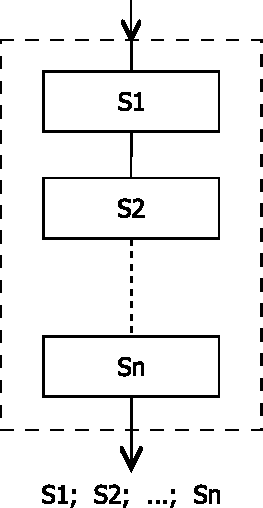
\includegraphics[scale=0.4]{chap1/fig1}}

这种分解的有效性，必须通过枚举推理确认。在这种情况下，要缩小程序与计算之间的概念距离，可以要求：一段线性排列的程序文本，按照子动作应当发生的次序，写出它们的名称或描述。前面的例子（$0 \leqslant r < dd$ 的不变性）
\medskip

{
	\setlength{\parindent}{8em}
	\hspace{-.4em}``$dd \coloneq dd/2;$
	
	\textbf{if} $dd \leqslant r$ \textbf{do} $r \coloneq r - dd$''
}
\medskip

\noindent
就满足这个条件。对计算的初层分解，是两个动作在时间上的相继执行；在程序文本中，我们能认出这个结构：
\medskip

{
	\setlength{\parindent}{8em}
	\hspace{-.4em}``将 $dd$ 减半；
	
	求 $r$ 对 $dd$ 的余数''。
}
\medskip

我们考虑的是全部满足 $0 \leqslant r < dd$ 的初始状态；对由此考虑的所有计算，以上分为两个子动作的分解都适用。到这里，一切都好。

不过，编写这段程序时假定：“求 $r$ 对 $dd$ 的余数”不是原子动作，而“从 $r$ 中减去 $dd$”是原子动作。考察“求 $r$ 对 $dd$ 的余数”期间所有可能发生的情况时，就有必要作出区分：有些情况下，会执行“从 $r$ 中减去 $dd$”；另一些情况下，$r$ 保持不变。写成
\medskip

{
	\setlength{\parindent}{8em}
	\hspace{-.4em}``\textbf{if} $dd \leqslant r$ \textbf{do} 从 $r$ 中减去 $dd$''
}
\medskip

\noindent
就表达了：在当前这个细节层次上，“求 $r$ 对 $dd$ 的余数”可以采取两种互斥形式之一；同时也给出了在两者之间作选择的依据。如果把“\textbf{if} $dd \leqslant r$ \textbf{do}”看作附加在“从 $r$ 中减去 $dd$”上的条件子句，那么把条件子句放在受它控制的语句前面，自然是合适的。（从这个意义上说，分支子句
\medskip

{
	\setlength{\parindent}{8em}
	\hspace{-.4em}``\textbf{if} 条件 \textbf{then} 语句 1 \textbf{else} 语句 2''
}
\medskip

\noindent
对“语句 1”和“语句 2”施加了“多余的次序”：它们仅仅是两个备选项，只是无法在线性媒介上同时表达。）

分支子句已经由 C. A. R. Hoare 推广；他的“case-of”结构可以在两个以上的可能项之间作选择。它们的流程图表示如下。

\centerline{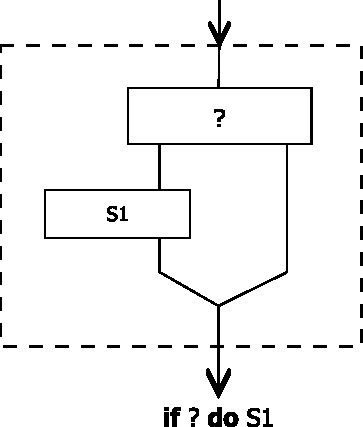
\includegraphics[height=11em]{chap1/fig2a}\qquad 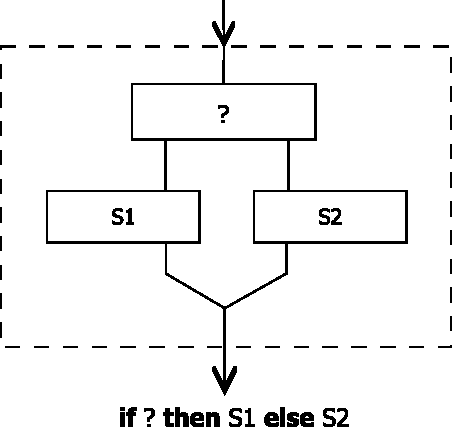
\includegraphics[height=11em]{chap1/fig2b}}

\centerline{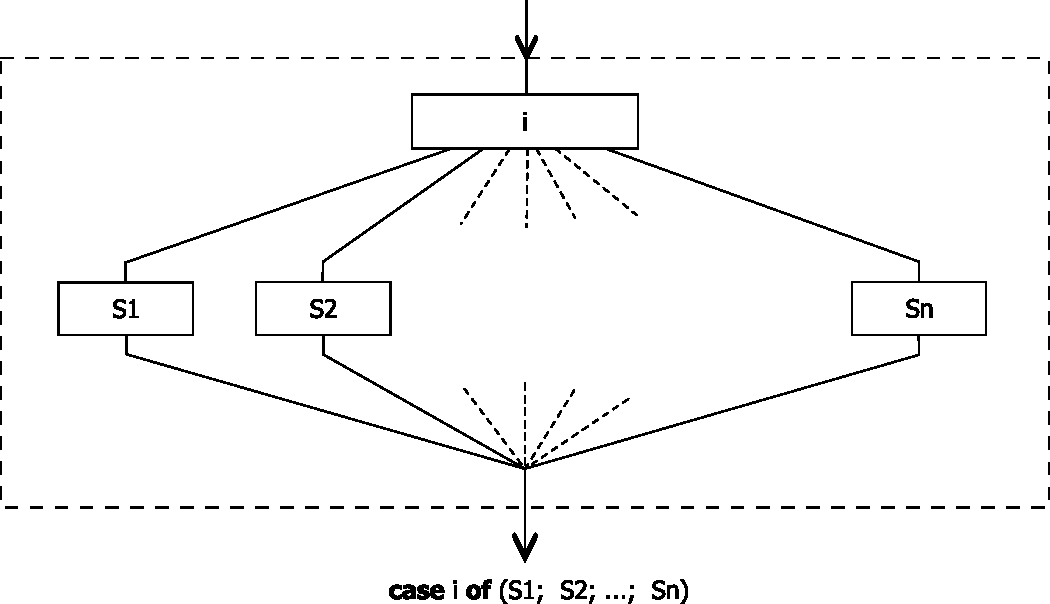
\includegraphics[width=.9\textwidth]{chap1/fig3}}

这些流程图具有一个共同性质：顶部只有一个入口，底部只有一个出口。正如虚线框所示，忽略虚线内的内容，就又可以把它们理解为顺序计算中的单个动作。更精确地说，我们处理的是大量可能的计算；对它们的初层分解，都得到相同的子动作时间序列。只有进一步检查\textemdash{}也就是查看虚线框内部\textemdash{}才会发现：在这组可能的计算中，这样一个子动作可以采取某个已列举的不同形式集合中的一种形式。

上述结构足以处理这样一类计算：它们在初层分解中，都分成同一组逐一列出的子动作。但对另一类计算，它们还不够：这类计算在初层分解中，子动作的数目会变化（即在所考虑的这一类计算之间变化）。这时，重复子句的用处就显现出来了。我们提到“\textbf{while} 条件 \textbf{do} 语句”和“\textbf{repeat} 语句 \textbf{until} 条件”，其流程图表示如下。

\centerline{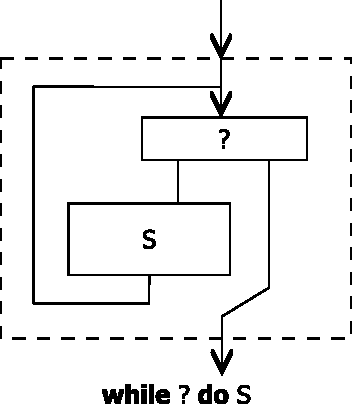
\includegraphics[height=11em]{chap1/fig4a}\qquad 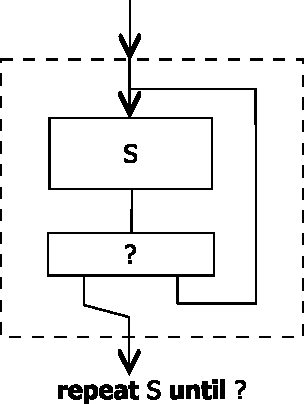
\includegraphics[height=11em]{chap1/fig4b}}

这些流程图同样具有顶部单一入口、底部单一出口的性质。它们让我们能够表达：虚线框所代表的动作，进一步检查后，是某一类型的子动作按时间顺序相继执行“足够多次”。

现在，我们已见到三种分解方式，分别可以叫作“串接”“选择”和“重复”。前两种靠枚举推理理解，最后一种靠数学归纳法理解。

如果程序仅用选择子句和重复子句控制执行顺序，那么它可以直接翻译到另一种程序设计语言中：该语言在其他方面都相同，只是执行顺序控制必须通过跳转到带标号的位置来表达。反过来却不成立。换句话说：与可以从任意程序块画箭头指向任意其他块的流程图相比，把自己限定在上述三种分解方式内，所得到流程图的拓扑结构受到限制。相对于那种更大的自由，只使用这些子句，就表现为一种执行顺序上的纪律。

我为什么建议遵守这种执行顺序纪律？这个决定的理由可以从许多方面说明。让我尝试几种说法，希望至少有一种能打动读者。

我们的最终目标之一，是让程序具有良好的结构，使理解程序所需的智力努力（以某种粗略意义衡量）与程序的长度（以另一种同样粗略的意义衡量）成正比。尤其要防止枚举推理的负担急剧增长。这项任务迫使我们采用古老格言“分而治之”的某种做法，也正是我们建议逐步分解计算的原因。

串接式分解可以通过枚举推理来理解。（前提是：在初层分解中，计算被拆分的子动作数量足够少，且对它们净效果的规格说明足够简明。我将在后面再谈这些要求；目前先假定条件已满足。）这样，根据程序文本对计算作出断言就是可行的，因为计算中的进展与程序文本中的进展之间，关系极其简单。特别是：如果进一步检查发现，某个子动作由选择子句或重复子句控制，这也不会加重理解初层分解的负担，因为在那一层，起作用的只有这个子动作的净效果。

由此可得：如果进一步检查发现某个子动作由选择子句控制，那么它具体走了哪条路径，在初层分解中始终无关紧要（唯一重要的是，它走了正确的路径）。同样，如果进一步检查发现某个子动作由重复子句控制，那么被重复的语句执行了多少次，这个数目本身也无关紧要（唯一重要的是，它重复了正确的次数）。

选择子句本身，也可以通过枚举推理理解；重复子句，则可以通过数学归纳法理解。对这三种分解方式\textemdash{}在我看来，这是一大帮助\textemdash{}我们都知道适用的推理模式。

所提出的执行顺序纪律，还有一个好处。理解程序时，我们要建立各种关系。在枚举推理的例子中，我们确认，程序段
\medskip

{
	\setlength{\parindent}{8em}
	\hspace{-.4em}``$dd: = dd/2;$
	
	\textbf{if} $dd \leqslant r$ \textbf{do} $r \coloneq r - dd$''
}
\medskip

\noindent
使关系
$$
0 \leqslant r < dd
$$

\noindent
保持不变。然而，即使我们能保证执行所引程序段之前这些关系成立，也不能断言它们始终成立；具体说，在所引的两条语句执行之间，它们未必成立。换言之，这些关系是否成立，取决于计算进行到了哪里；这似乎是顺序过程的典型特征。

类似地，我们还会赋予变量某种含义：一个变量可能用于计数某类事件发生的次数，比如当前页已经打印的行数。转到下一页之后，立即将它重置为零；打印一行之后，立即加 1。同样，在重置或递增这个计数之前，“当前页已经打印的行数”这一解释是不成立的。因此，赋予变量这样的含义，也只能相对于计算的进展来做。这一观察引出一个问题：“怎样刻画计算的进展？”

简而言之，我们要找一个坐标系，以便标识计算进展中的离散位置；而且希望这个坐标系独立于那些在程序控制下被操作的变量。如果需要用这些变量的值来描述计算进展，我们就陷入了循环论证，因为我们恰恰是想相对于这种进展来解释这些变量的含义。

（还有一个更强的理由说明不应依赖变量的值：设某个程序含有一个不终止的循环，它在有限个不同状态之间反复运行。永远循环的原因在于，计算进展中的不同位置可以处于\textit{同一个}状态。如此一来，状态显然不能区分这两个\textit{不同的}进展位置！）

我们可以换一种方式说明这个问题。给定一个正在运行的程序，假定计算尚未完成，就在某个离散的进展位置停了下来。我们怎样标识这个中断位置？例如，若想把计算重新做到完全相同的位置，该怎么办？又或者，如果停止是由某种运行时错误引起的，我们怎样才能在不完整转储存储器的情况下，标识当时的进展位置？

为简单起见，假定程序文本在（线性的）文本空间中展开，并假定有一种标识机制，用来标识与计算进展的离散位置相对应的程序位置；我们把这种机制叫作“文本索引”。（如果计算进展的离散位置位于相邻两次语句执行之间，那么文本索引所标识的，例如可以是分号。）文本索引是一种广义的指令计数器，其值指向文本中的一个位置。

如果只采用串接和选择进行分解，那么单个文本索引就足以标识计算进展。加入重复子句之后，文本索引就不足以描述计算进展了。不过，每次进入一个重复子句，系统可以引入一个所谓的“动态索引”，严格计数当前相应重复的序号；重复终止时，系统再移除对应的动态索引。由于重复子句可以相互嵌套，合适的机制是栈（即后进先出的存储器）。最初栈为空；进入重复子句时，把一个新的动态索引（置为零或一）放到栈顶；每当决定继续重复，就将栈顶元素加 1；每当决定结束重复，就移除栈顶元素。（这种安排十分清楚地反映了：重复终止之后，重复的次数，甚至它曾经是一个重复这一事实，都不再重要。）

一旦程序设计语言允许使用过程，单个文本索引就不够了。如果文本索引指向某个过程体内部，那么只有同时说明指的是该过程的哪一次调用，才能刻画计算的动态进展；而这可以通过给出一个指向调用位置的文本索引来做到。引入过程后，文本索引必须推广为文本索引栈：调用过程时增加一个元素，过程返回时减少一个元素。

关键在于，这些索引的值不受程序员控制。不论他是否愿意，它们都由程序的书写形式或当前计算的动态演进所定义。它们提供了一套独立坐标，用来描述计算进展；在这个“独立于变量”的参照系中，可以给变量赋予含义。

当然，即便自由使用跳转，也存在一个独立于程序员的坐标系，可以用来唯一描述顺序计算的进展：一种规范化的时钟，计数从程序开始起经过了多少个“计算进展的离散位置”。它确实能唯一标识位置，却完全无助于理解，因为文本索引已不再是这个坐标系的组成部分。

这里的教训是：如果承认自己有责任借助引发计算的程序文本，在智力上掌握这些计算，那么我们就应当谦逊地把自己限定在最系统的执行顺序机制内，确保“计算中的进展”以最直接的方式映射到“文本中的进展”。

\section[论程序的比较]{论程序的比较}
\label{sec:comparing-programs}

程序员在日常工作中经常遇到这样的情况：对于一个给定问题，即使已指定用某个算法求解，又指定了机器，程序仍远非唯一确定。设计过程中，他必须在不同方案间选择；得到一个正确程序之后，也经常需要修改它。例如，人们可能觉得，另一个方案的计算对现有设备资源的要求更合适。

这些情况引出了程序等价性的问题：给定两个程序，它们是否引发净效果相同的计算？如果对程序的给定方式、执行这些计算的机器，以及计算的“净效果”都作适当形式化，这大概可以成为一个表述明确、能吸引某些数学头脑的问题。但我不打算以这种一般形式处理它。恰恰相反，我并不是从两个任意给定的程序出发——例如由两个作者独立构思的程序；我关心的是那些可以视为同一个人思考结果的不同程序方案。于是，问题变成：怎样构思这两个方案，并安排它们的结构，才能使比较工作更容易？

我做过许多试验，从中得到的基本经验可以概括如下：两个程序若引发净效果相同的计算，它们便\textit{在这个意义上}等价，而\textit{不能事先认定}它们在其他任何意义上也等价。当我们想通过比较程序，来比较其对应的计算时，基本经验是：如果在所比较的层次上，两个程序中的执行顺序不同，那么比较就不可能进行，或者徒劳、无趣、极其困难——随你怎么说。更明确地说：只有当成对的计算能分解为按时间相继发生、彼此能够对应的动作，而相应程序文本也能同样分解为分别对应这些动作的指令时，比较这两个程序及它们可能引发的计算才有吸引力。

这是一个很强的条件。先举一个例子。

排除布尔条件检查的副作用，并假定“$B2$”的值不变（即执行“$S1$”或“$S2$”都不影响它），\textit{我们}可以确认以下两个程序等价：
\begin{equation}
	\label{eq:comparing-example-1}
	\begin{split}
	&\text{\hspace{-.4em}``\textbf{if }} B2\text{ \textbf{then}}\\
	&\quad \text{\textbf{begin while} } B1\text{ \textbf{do} } S1 \text{ \textbf{end}}\\
	&\text{\textbf{else}}\\
	&\quad \text{\textbf{begin while} } B1\text{ \textbf{do} } S2\text{ \textbf{end}''}
	\end{split}
\end{equation}

\noindent
以及
\begin{equation}
	\label{eq:comparing-example-2}
	\begin{split}
		&\text{\hspace{-.4em}``\textbf{while }} B1\text{ \textbf{do}}\\
		&\text{\textbf{begin if} } B2\text{ \textbf{then} } S1\text{ \textbf{else} } S2\text{ \textbf{end}''}
	\end{split}
\end{equation}

\label{pg:dilema}
第一个结构在初层上由选择子句控制执行顺序，第二个结构在初层上由重复子句控制执行顺序。我能够确认这些计算的输出等价，却不能在其他任何有用的意义上把它们看作等价。我不得不强迫自己接受这个结论：式（\ref{eq:comparing-example-1}）和式（\ref{eq:comparing-example-2}）“难以比较”。起初，这个结论让我非常恼火。后来，我逐渐把这种不可比性看作生活中的一个事实，也因此把它视为一个主要理由：在式（\ref{eq:comparing-example-1}）和式（\ref{eq:comparing-example-2}）之间选择，是一项相关的设计决定，不应未经仔细考虑就作出。正是它表面上的微不足道，使我留意到哪些因素应当影响这种选择。这些因素超出了本节范围，但我希望后面再谈。

再举一个稍微隐蔽些的不可比例子。

给定两个数组 $X[1:N]$ 和 $Y[1:N]$，以及布尔变量“equal”，要求编写程序，给“equal”赋予这样的布尔值：“两个数组逐元素相等”。空数组（即 $N = 0$）视为相等。

引入变量 $j$，并给“equal”赋予“前 $j$ 对元素中尚未发现差异”的含义，我们可以写出以下两个程序。
\begin{equation}
	\label{eq:comparing-example-3}
	\begin{split}
		&\text{\hspace{-.4em}``}j \coloneq 0;\text{ equal} \coloneq \text{\textbf{true}};\\
		&\text{\textbf{while} } j \neq N\text{ \textbf{do}}\\
		&\quad\text{\textbf{begin} } j \coloneq  j + 1;\text{ equal} \coloneq \text{equal \textbf{and} } (X[j] = Y[j]) \text{ \textbf{end}''}
	\end{split}
\end{equation}

\noindent
以及
\begin{equation}
	\label{eq:comparing-example-4}
	\begin{split}
		&\text{\hspace{-.4em}``}j \coloneq 0;\text{ equal} \coloneq \text{\textbf{true}};\\
		&\text{\textbf{while} } j \neq N\text{ \textbf{and} equal \textbf{do}}\\
		&\quad\text{\textbf{begin} } j \coloneq  j + 1;\text{ equal} \coloneq (X[j] = Y[j]) \text{ \textbf{end}''}
	\end{split}
\end{equation}

程序（\ref{eq:comparing-example-4}）与程序（\ref{eq:comparing-example-3}）的不同在于：一旦发现某一对元素不同，就终止重复。对于同一输入，两个程序的重复次数可能不同；因此，只有把程序最后两行视为描述一个整体动作、不再拆成子动作时，它们才在我们所说的意义上可比。但是，如果确实希望考虑两者都以重复结束这一事实，它们又有什么关系？为了弄清楚，我们来证明这两个程序的正确性。

对于数组 $X$ 和 $Y$，可以在 $0 \leqslant j \leqslant N$ 上定义如下 $N + 1$ 个函数 $\text{EQUAL}_j$：
\begin{equation}
	\label{eq:comparing-example-5}
	\begin{split}
		\text{当 } j = 0\qquad & \text{EQUAL}_j = \text{\textbf{true}} \\
		\text{当 } j > 0\qquad  & \text{EQUAL}_j = \text{EQUAL}_{j-1}\text{ \textbf{and} } (X[j] = Y[j]).
	\end{split}
\end{equation}

用这些函数表达，要求建立的净效果是
$$
\text{equal} = \text{EQUAL}_N.
$$

两个程序都维持关系
\begin{equation}
	\text{equal} = \text{EQUAL}_j
\end{equation}

\noindent
其中 $j$ 从 $0$ 开始递增。

我们很容易想把程序（\ref{eq:comparing-example-3}）和程序（\ref{eq:comparing-example-4}）看成同一个（抽象）程序（\ref{eq:comparing-example-7}）的两种细化：
\begin{equation}
	\label{eq:comparing-example-7}
	\begin{split}
		&\text{\hspace{-.4em}``}j \coloneq 0;\text{ equal} \coloneq \text{EQUAL}_0;\\
		&\text{\textbf{while} ``可能仍有：equal} \neq \text{EQUAL}_N\text{'' \textbf{do}}\\
		&\quad\text{\textbf{begin} } j \coloneq  j + 1;\text{ ``equal} \coloneq \text{EQUAL}_j\text{'' \textbf{end}''}
	\end{split}
\end{equation}

\noindent
其中，“可能仍有：equal $\neq$ EQUAL$_N$”代表某种尚未具体确定的基本操作。对它求值时，
$$
\text{equal} = \text{EQUAL}_j
$$

\noindent
成立；程序（\ref{eq:comparing-example-3}）和程序（\ref{eq:comparing-example-4}）的区别，在于它们用不同的判据保证“equal”取得最终值 EQUAL$_N$。

程序（\ref{eq:comparing-example-3}）中的判据很朴素，即
$$
j = N.
$$

\noindent
在被重复的语句开始时，
$$
\text{equal} = \text{EQUAL}_j
$$

\noindent
仍然成立。因此，执行“$j \coloneq j + 1$”之后，
$$
\text{equal} = \text{EQUAL}_{j-1}
$$

\noindent
成立；于是赋值语句
$$
\text{``equal} \coloneq \text{equal \textbf{and} } (X[j] = Y[j])\text{''}
$$

\noindent
就直接是递推关系（\ref{eq:comparing-example-5}）的转写。

要得到程序（\ref{eq:comparing-example-4}），则需要分析递推关系（\ref{eq:comparing-example-5}）。从中可以（再次用数学归纳法）推出，$\text{EQUAL}_j = \text{\textbf{false}}$ 蕴含 $\text{EQUAL}_N = \text{\textbf{false}}$，所以 $\text{EQUAL}_j = \text{\textbf{false}}$ 蕴含 $\text{EQUAL}_j = \text{EQUAL}_N$。如果出现这种情况，也能保证等式“$\text{equal} = \text{EQUAL}_N$”，由此便得到程序（\ref{eq:comparing-example-4}）。程序（\ref{eq:comparing-example-4}）中，被重复语句需要处理的（子）计算集合，限定为初始状态满足“$\text{equal} = \text{\textbf{true}}$”的那些计算。因此，在程序（\ref{eq:comparing-example-4}）中，赋值“$\text{equal} \coloneq \text{EQUAL}_j$”可以简写为
$$
\text{``equal} \coloneq (X[j] = Y[j])\text{''}
$$

现在就清楚了：为什么把式（\ref{eq:comparing-example-7}）引入为式（\ref{eq:comparing-example-3}）和式（\ref{eq:comparing-example-4}）的抽象，会造成误导。用“可能仍有：equal $\neq \text{EQUAL}_N$”，我们说明了某个布尔表达式为真和为假的含义，却没有给出表达式本身，这是很危险的。我们试图把式（\ref{eq:comparing-example-7}）理解成一个程序，在它自身的层次上，部分执行顺序尚未定义，而且随不同细化而变化。因此，我们试图把式（\ref{eq:comparing-example-7}）的最后几行同时看作式（\ref{eq:comparing-example-3}）和式（\ref{eq:comparing-example-4}）最后几行的模型；但这会误导，因为它们引发的计算无法建立一一对应关系。

关于我们认为不可比的程序，就谈到这里。可比程序的例子将在后面几节中出现。最后补充一句：我们说过，“成对的计算可以分解为按时间相继发生、彼此能够对应的动作”。但我们并未要求，配对动作的净效果必须相同！我们既可以比较完成同一工作的不同程序方案，也可以比较完成相似工作的不同程序。

\section[逐步构造程序的第一个例子]{逐步构造程序的第一个例子}
\label{sec:first-example-step-wise-program-composition}

在“\nameref{sec:undertanding-programs}”一节中，我强调了系统地安排执行顺序的必要性，使计算的结构能够体现在程序结构中；这样，我们就可以说，程序与计算共同形成结构。本节将尝试为“安排计算的结构”这个仍较模糊的概念，增添一些具体内容。这是第一次尝试：利用抽象能力，减轻枚举推理的负担；同时，它也将一以贯之地运用“\nameref{sec:undertanding-programs}”一节中提到的分解方式。

我不打算拿一个现成产品来展示所谓结构良好的程序，而要非常详细地描述这样一个程序的构造过程。这样做，是因为程序并不是现成存在的，恰恰相反，它们必须由人构造。我特别感兴趣的程序，是那些在我看来与我们的构造能力和理解能力相当适合的程序。

任务是指示计算机打印一张前一千个素数的表，规定 2 是第一个素数。

\begin{enumerate}[leftmargin=*, itemindent=2.2\parindent, label=\textit{注 }\arabic*.]
	\item 选择这个例子，是因为一方面，它足够困难，可以作为程序设计中某些问题的模型；另一方面，它的数学背景又简单、熟悉，不至于让问题本身占据我们的全部注意力。
	
	\item 我并不声称最终程序会是“最好的”，无论读者愿意用什么尺度来衡量。在本说明的先前版本中，余数是用除法计算的。至少两位读者对此反应激烈：“谁都知道，生成素数最有效的方法是埃拉托色尼筛法。”于是，他们再也读不下去了！
\end{enumerate}

我的基本做法，是以极小的步子构造程序，每次尽可能少作决定。问题分析逐渐深入，程序也随之进一步细化。

要构造一个算法，就必须用那些与我们已经充分理解的指令集合相对应的动作，组成所需要的计算。

程序最简单的形式是
\medskip


\noindent
描述 0：
\labeltext{描述 0}{tx:description-0}

\textbf{begin} “打印前一千个素数” \textbf{end}

\noindent
如果“打印前一千个素数”指的是那套已充分理解的指令集合中的一条指令，那么\ref{tx:description-0}就解决了问题。为了继续讨论，假定这条指令\textit{不在}该指令集合中。因此，我们必须构想一个由“更基本”的动作组成的计算，产生所期望的净效果。第一个方案是把素数生成与打印分开，于是提出\ref{tx:description-1}：
\medskip

\textbf{begin variable} “表 $p$”；
\labeltext{描述 1}{tx:description-1}

\quad “将前一千个素数填入表 $p$”；

\quad “打印表 $p$”

\textbf{end}，

\noindent
这表明，计算由两个按时间相继发生的动作组成，而且发生在只含一个变量的状态空间中，该变量叫作“表 $p$”。第一个动作给它赋值；第二个动作由它当时的值控制。

同样，如果“将前一千个素数填入表 $p$”与“打印表 $p$”都在那套已充分理解的指令集合中，而且“表 $p$”也是隐含可用的资源，那么问题就解决了。为继续讨论，我们再次假定并非如此。这意味着，下一步细化时，必须说明如何通过另外两个（子）计算产生这两个动作的效果。此外，还必须决定：怎样表示“表 $p$”的中间值所包含的信息——这个对象目前还相当不明确。

在继续之前，我想强调：写下描述 1 时，我们作出的决定有多么少，考虑到原始问题说明的内容又有多么少。我们假定某种形式的“表 $p$”资源可用，因此能在开始打印前，算出前一千个素数。在这个假定下，我们利用了一个事实：素数的计算可以独立于打印来构思。对于原始问题说明，除此以外，我们考虑的内容大体只限于：至少存在一千个不同的素数（要使问题说明有意义，就必须假定这一点）。在这个阶段，“素数”这个概念究竟是什么意思，仍然不太重要。对于打印输出的具体版式要求，我们也完全没有作出承诺。显然，这种做法的优点在于：原始问题中这两个相当独立的方面所带来的后果，似乎已经分别归入两个组成动作各自的细化中。这表明，在应用“分而治之”这一黄金原则时，我们多少取得了成功。

不过，继续讨论时，我们必须问自己：现在，这两个子计算究竟能在多大程度上彼此独立地构思？更精确地说：“我们是否已经达到这样的阶段：可以让两位程序员互不依赖地设计两个子算法，以引发相应的子计算？”

既然这两个动作已不能视为由充分理解的指令所调用，那么变量“表 $p$”也就不能再视为隐含可用的资源。正如必须把动作分解为子动作，我们也必须选择怎样组成变量“表 $p$”：选择什么数据结构，来表示从第一个动作经由“表 $p$”传递给第二个动作的信息。这个决定总得在某个时刻作出，问题在于：“什么时候？”以及“怎样作出？”

原则上，似乎有两条路。第一条是尽量推迟决定如何把“表 $p$”组织成一些更中性、较少依赖特定问题的部件。如果推迟对“表 $p$”结构的决定，下一步就要细化一个或两个动作。为此，可以假定在这个仍然神秘的对象\mbox{“表 $p$”}上存在一套合适的操作；最后，再汇总这些操作，根据它们的要求，设计最合适的“表 $p$”结构。

另一条路，是尝试就在此时此地决定“表 $p$”的结构。一旦前一千个素数表的表示方式确定下来，两个动作的细化就能相当独立地进行。

两条路都棘手。例如，第一个子计算的算法是否合适，很大程度上取决于所假定的“表 $p$”操作能否容易、优雅地实现；如果其中一个或几个操作笨拙到无法接受，整座大厦就会倒塌。反过来，如果过早决定“表 $p$”的结构，也很可能发现子计算随后变得别扭。这个问题无法绕开：在优雅的程序中，“表 $p$”的结构与引用它的计算必须相互匹配。我认为，高效程序员的行为可以这样描述：努力先作最容易的决定，即用尽可能少的探究——试错、反复相互调整等——获得尽可能充分的理由，相信自己将来不会后悔这个决定。

为了不让这番讨论过分冗长，我们假定程序员鼓起勇气，决定现在首先确定“表 $p$”的结构。一旦采取这个立场，立即会出现两种方案。一方面，我们可以利用这样的事实：“前 1000 个素数的表”不只是一张含有一千个数的表——不像工厂里 1000 名员工的月工资表——它的所有数还互不相同。利用这一点，可以用线性布尔数组组织信息，将连续的数组元素对应于连续的自然数，指示相应自然数是否为素数。数论给出第一千个素数数量级的估计，由此可以界定一个足够长的数组长度。如果这样组织数据，就准备了一个容易回答“$n$（小于最大值）是否为素数？”的机制。另一方面，我们可以选择整数数组，依次列出素数。（如果需要\textit{事先}给定整数数组元素的最大值，这里也会用到数论得到的同一个估计。）后一种形式，则建立了适合回答“第 $k$ 个素数的值是什么，其中 $k \leqslant 1000$？”的机制。

我们让程序员勇敢地选择后一种表示。这对打印操作似乎很合适，因为要求的是打印素数，而不是打印自然数并标记它们是不是素数。对计算阶段，它也似乎很合适；这里要给程序员一点预见：分析一个自然数是否为素数，会与能否找到这个数的素因子有关。

于是，程序细化的下一阶段，是仔细说明这个仍然神秘的对象“表 $p$”采用何种表示约定，并按这一约定重新定义两个操作。

约定如下：“表 $p$”中的信息，由“\textbf{integer array} $p[1 : 1000]$”各元素的值表示；当素数按数值递增顺序排列时，对 $1 \leqslant k \leqslant 1000$，$p[k]$ 等于第 $k$ 个素数。（如果整数的最大值已隐含给定，我们假定数论能让我们断定它足够大。）

现在，要描述这一新的细化，就遇到一个新困难。\ref{tx:description-1}之所以能写成单个程序，是因为它细化的是\ref{tx:description-0}中的单个已命名动作“打印前一千个素数”。（用更常见的说法，\ref{tx:description-1}可以写成一个过程体。）但下一层不再如此：我们必须在某种意义上同时细化三个已命名的实体——“表 $p$”和两个动作。因此，需要想出一套标识用语，说明什么细化了什么。

为继续讨论，我们暂时作一个试探性的建议：\ref{tx:description-0}是一段有效文本，用单个已命名动作“打印前一千个素数”来表达；用代码 $0a$ 标识这个动作。

\hyperref[tx:description-1]{描述 1}之所以称为“\hyperref[tx:description-1]{1}”，是因为它是\ref{tx:description-0}的下一层细化。它细化了 $0a$\textemdash{}\ref{tx:description-0}唯一使用的项\textemdash{}自身则用三个已命名实体表达；我们给它们附上代码：

\noindent
“表 $p$”\hfill 1a

\noindent
“将前一千个素数填入表 $p$”\hfill 1b

\noindent
“打印表 $p$”\hfill 1c

\noindent
代码以 1 开头，因为\ref{tx:description-1}是用它们表达的；“a”“b”“c”则用于区分。

现在必须描述“表 $p$”内信息所采用的表示约定，而这个约定涉及 1a、1b、1c 三个元素。因此，把它叫作\ref{tx:description-2}；其中应分别描述三个元素（用等号作分隔符）：
\medskip

\noindent
描述 2：
\labeltext{描述 2}{tx:description-2}
\nopagebreak

\noindent
1a $=$ “\textbf{integer array} $p[1 : 1000]$”

\noindent
1b $=$ “对 $k$ 从 1 到 $1000$，使 $p[k]$ 等于第 $k$ 个素数”

\noindent
1c $=$ “对 $k$ 从 1 到 1000，打印 $p[k]$”。

\hyperref[tx:description-2]{描述 2}用三个已命名实体表达，按显而易见的次序，赋予它们代码 2a、2b、2c。（就代码而言，\ref{tx:description-2}内容很少：它只是说，对 1a、1b、1c，我们分别选择了细化 2a、2b、2c。）

\noindent
\textit{说明}。在表示“表 $p$”内的信息时，我们没有利用每个待打印的值只出现一次这个事实，也没有利用它们按数值递增顺序出现这个事实。反过来，这意味着：名为 2c 的动作，被看作“打印任意一组一千个整数值”的一个具体实例（它也可以是一千名编号员工的月工资表！）。这个例子中，打印动作的净效果，与前一千个素数一样，是唯一确定的；但我们把它构想成某个更大事件类别中的具体实例。进一步细化 2c 时，处理的是整个类别；这一类中的具体实例，则由数组 $p$ 各元素的值确定。当人们说“定义接口”时，我常觉得，他们忽略了其中预设的推广，忽略了对一类“可能”动作的构想。

如果 2b 和 2c 都在那套已充分理解的指令集合中（于是 2a 也是隐含可用的资源），整个问题就解决了。为继续讨论，再次假定并非如此。于是，我们需要为动作 2b 和 2c 构想子计算。但现在，由于引入了第 2 层，2b 与 2c 各自的细化可以独立设计。

\emph{2b 的细化：“对 $k$ 从 $1$ 到 $1000$，使 $p[k]$ 等于第 $k$ \emph{个}素数”}。

我们要找的是描述 2b1，即 2b 的第一次细化。为了表明 2b 与 2c 的细化彼此独立，我们在 2b 后另起编号，而不把下一个描述叫作“3 什么”。

在描述 2b1 中，要给出一个算法，描述数组 $p$ 各元素怎样得到自己的值。例如，这意味着必须说明赋值的顺序。第一次细化时，我们就只说明这一点，最好不说明其他事情。一个显而易见却荒唐的版本，开头如下（“版本号”放在括号里）：

\noindent
2b1(l)：
\nopagebreak

\noindent
\textbf{begin} $p[1] \coloneq 2$; $p[2] \coloneq 3$; $p[3] \coloneq 5$; $p[4] \coloneq 7$; $p[5] \coloneq 11$;\ \dots\ \textbf{end}

\noindent
这意味着程序员已经知道前一千个素数的表。我们不再考虑这个版本，因为这就意味着程序员几乎根本不需要机器。

第一个素数已给定 $(=2)$，并假定程序员不知道第一千个素数。于是，填充数组 $p$ 各元素最自然的顺序，似乎就是下标递增的顺序。如果只表达这一点，例如可以得到

\noindent
2b1(2)：

\noindent
\textbf{begin integer} $k$, $j$; $k \coloneq 0$; $j \coloneq 1$;

\noindent
\quad \textbf{while} $k < 1000$ \textbf{do begin} “增加 $j$，直到下一个素数”；

\noindent
\quad\quad $k \coloneq k + 1$; $p[k] \coloneq j$ \textbf{end}

\noindent
\textbf{end}

把 $k$ 理解为已找到的素数个数，并核实第一个素数 $(=2)$ 确实是大于 1（$=$ $j$ 的初始值）的最小素数，就很容易用数学归纳法证明 2b1(2) 正确（假定存在足够多的素数）。

如果“增加 $j$，直到下一个素数”所描述的操作——称为 2b1(2)a——在指令集合中，那么描述 2b1(2) 就是一个完善的程序。但假定它不在。这样，下一次细化时，就必须表达怎样增加 $j$（同样，最好不表达其他事情）。于是得到第 2b2(2) 层的描述：

\noindent
2b1(2)a $=$

\noindent
\textbf{begin boolean} $j$prime;

\noindent
\quad \textbf{repeat} $j \coloneq j + 1$;

\noindent
\quad\quad “赋予 $j$prime 这样的含义：$j$ 是素数”

\noindent
\quad \textbf{until} $j$prime

\noindent
\textbf{end}

\noindent
\textit{说明}。这里使用 repeat-until 子句，是为了表明 $j$ 总要至少增加一次。

其正确性同样几乎无可怀疑。不过，如果假定程序员知道除 2 以外的所有素数都是奇数，那么由于效率低，他大概不会满意这个版本。为这种“缺乏预见”所付出的代价，就是修改版本 2b1(2)。单独处理素数 2 之后，循环就只需处理奇素数。替代 2b1(2)，我们得到

\noindent
2b1(3)：

\noindent
\textbf{begin integer} $k$, $j$; $p[1] \coloneq 2$; $k \coloneq 1$; $j \coloneq 1$;

\noindent
\quad\textbf{while} $k < 1000$ \textbf{do}

\noindent
\quad\quad\textbf{begin} “增加奇数 $j$，直到下一个奇素数”；

\noindent
\quad\quad\quad $k \coloneq k + 1; p[k]: = j$

\noindent
\quad\quad\textbf{end}

\noindent
\textbf{end}

\noindent
对引号中的操作——姑且称为“2b1(3)a”——作类似细化，得到第 2b2(3) 层的描述：

\noindent
2b1(3)a $=$

\noindent
\textbf{begin boolean} $j$prime;

\noindent
\quad\textbf{repeat} $j \coloneq j + 2;$

\noindent
\quad\quad“对于奇数 $j$，赋予 $j$prime 这样的含义：$j$ 是素数”；

\noindent
\quad\textbf{until} $j$prime

\noindent
\textbf{end}

刚才在两个描述层次间来回调整，实质上不过是为了方便，调整总体结构与必须适合这个结构的基本操作之间的接口。这种往复调整、这种试错方式，确实不理想；但当我们缺乏预见、又不得不依次作决定时，我看不到别的办法。可以把这些努力看作一些试验：以相当低的代价，探索接口大概选在哪里最方便。

\noindent
\textit{说明}。2b1(2) 和 2b1(3) 都可以粗略描述为

\noindent
\textbf{begin} “将表 $p$ 和 $j$ 设为初始值”；

\noindent
\quad\textbf{while} “表 $p$ 尚未填满” \textbf{do}

\noindent
\quad\textbf{begin} “增加 $j$，直到下一个待加入的素数”；

\noindent
\quad\quad “将 $j$ 加入表 $p$”

\noindent
\quad\textbf{end}

\noindent
\textbf{end}

\noindent
但我们不这样做，因为两个版本的执行顺序不同（参见“\nameref{sec:comparing-programs}”），我们把它们看作“不可比”。选择 2b1(3)，就意味着认定试用版本 2b1(2) 和 2b1(1) 一样，不再适用，因此舍弃。

从 2b1(2) 改为 2b1(3)，理由是更深的细化层次能获得效率收益。这项收益在第 2b2 层获得，因为现在 $j$ 可以每次加 2；在 2b2(3) 层尚未确定的基本操作中，这项收益也会体现出来：用于“对于奇数 $j$，赋予 $j$prime 这样的含义：$j$ 是素数”的算法，只需分析 $j$ 的奇数值。

再说一次：在 2b2(3) 中，我们用一个算法细化了 2b1(3)。只要“对于奇数 $j$，赋予 $j$prime 这样的含义：$j$ 是素数”——称为“2b2(3)a”——在那套已充分理解的指令集合中，这个算法就解决了问题。现在假定它不在；换句话说，需要引发一个计算，判断给定的奇数 $j$ 是否有因子。直到这一步，代数才真正进入讨论。这里，我们利用已知事实：只需尝试素因子；而且，待试的素数都已经能在数组 $p$ 已填充的部分中找到。

我们使用以下事实：

\begin{enumerate}[wide, nosep, label=(\arabic*)]
	\item $j$ 是奇数，因此应尝试的最小潜在因子为 $p[2]$，即大于 2 的最小素数。

	\item 如果 $p[\text{ord}]$ 是平方大于 $j$ 的最小素数，那么应尝试的最大素数是 $p[\text{ord} - 1]$。
\end{enumerate}

（这里，我还用了一个事实：平方大于 $j$ 的最小素数已经可以在表 $p$ 中找到。对这个程序的一个早期版本，我把这一点视为当然；以下怀着谦逊，引用 Don Knuth 当时的评论：

\begin{addmargin}[\parindent]{0em}
“这里你犯了一个严重的遗漏！你的程序使用了一个深刻的数论结果：如果 $p_n$ 表示第 $n$ 个素数，那么\textit{总有}
\end{addmargin}
$$
p_{n+1}<p_n^2.\text{”}
$$

\noindent
我认错。）

如果这个集合非空，我们就有机会找到因子；一旦找到因子，就可以停止考察这个 $j$ 值。必须决定按什么顺序尝试集合中的素数；我们选数值递增顺序，因为素数越小，成为 $j$ 因子的概率越大。

当 ord 的值已知时，可以为“对于奇数 $j$，赋予 $j$prime 这样的含义：$j$ 是素数”给出第 2b3(3) 层的描述：

\noindent
2b2(3)a =

\noindent
\textbf{begin integer} $n$; $n \coloneq 2$; $j$prime $\coloneq$ \textbf{true};

\noindent
\quad\textbf{while} $n <$ ord \textbf{and} $j$prime \textbf{do}

\noindent
\quad\textbf{begin} “赋予 $j$prime 这样的含义：$p[n]$ 不是 $j$ 的因子”；$n \coloneq n + 1$

\noindent
\quad\textbf{end}

\noindent
\textbf{end}

但这个版本假定，作为 $j$ 的函数，ord 的值已经知道。我们本来也可以这样开始细化：

\noindent
\textbf{begin integer} $n$, ord;

\noindent
\quad ord $\coloneq 1$; \textbf{while} $p[\text{ord}] \uparrow 2 \leqslant j$ \textbf{do} ord $\coloneq$ ord $+ 1$;

\noindent
\quad \dots

\noindent
即每次需要“ord”的值，都重新计算。这里似乎适合用存储空间换取计算时间：与其每次需要这个函数就重新计算，不如引入一个额外变量 ord，保存它的当前值。设置 $j$ 时要设置它，改变 $j$ 时要调整它。

可惜，这迫使我们重新编写一些程序。一种办法是：在引入 $j$ 的同时引入整数变量 ord，然后扫描程序，在每个操作 $j$ 的地方插入适当的 ord 操作。我不喜欢这种做法，因为在引入 $j$、并赋予它含义的那一层，函数“ord”无关紧要。因此，我们将努力只在合适的层次引入 ord，并且非常谨慎。

对于 2b：“对 $k$ 从 1 到 1000，使 $p[k]$ 等于第 $k$ 个素数”，我们写下（与第 2b1(3) 层类似）

\noindent
第 2b1(4) 层：

\noindent
\textbf{begin integer} $k$, $j$; $p[1] \coloneq 2$; $k \coloneq 1$;

\noindent
\quad “将 $j$ 置为一”；

\noindent
\quad\textbf{while} $k < 1000$ \textbf{do}

\noindent
\quad\textbf{begin} “增加奇数 $j$，直到下一个奇素数”；

\noindent
\quad\quad $k \coloneq k + 1$; $p[k] \coloneq j$

\noindent
\quad\textbf{end}

\noindent
\textbf{end}

\noindent
它用以下实体表达：

\noindent
2b1(4)a\tabto{5em} “增加奇数 $j$，直到下一个奇素数”

\noindent
2b1(4)b\tabto{5em} “将 $j$ 置为一”。

在下一层，只引入 2b1(4)a 的子计算；另一个则向下传递。

\noindent
第 2b2(4) 层：

\noindent
2b1(4)a $=$

\noindent
\textbf{begin boolean} $j$prime;

\noindent
\quad\textbf{repeat} “将 $j$ 加二”；

\noindent
\quad\quad “对于奇数 $j$，赋予 $j$prime 这样的含义：$j$ 是素数”

\noindent
\quad\textbf{until} $j$prime

\noindent
\textbf{end;}

\noindent
2b1(4)b $=$ 2b2(4)b

\noindent
它用以下实体表达：

\noindent
2b2(4)b\tabto{5em} 仍表示“将 $j$ 置为一”

\noindent
2b2(4)c\tabto{5em} “将 $j$ 加二”

\noindent
2b2(4)d\tabto{5em} “对于奇数 $j$，赋予 $j$prime 这样的含义：$j$ 是素数”。

直到下一层，我们才需要谈 ord。因此，现在写下

\noindent
第 2b3(4) 层：\textbf{integer} ord;

\noindent
2b2(4)b =

\noindent
\textbf{begin} $j \coloneq 1$; “设置 ord 的初始值” \textbf{end};

\noindent
2b2(4)c =

\noindent
\textbf{begin} $j \coloneq j + 2$; “调整 ord” \textbf{end};

\noindent
2b2(4)d =

\noindent
\textbf{begin integer} $n$; $n \coloneq 2$; $j$prime $\coloneq$ \textbf{true};

\noindent
\quad\textbf{while} $n <$ ord \textbf{and} $j$prime \textbf{do}

\noindent
\quad\quad\textbf{begin} “赋予 $j$prime 这样的含义：$p[n]$ 不是 $j$ 的因子”；

\noindent
\quad\quad\quad $n \coloneq n + 1$

\noindent
\quad\textbf{end}

\noindent
\textbf{end}

\noindent
它用以下实体表达：

\noindent
2b3(4)a\tabto{5em} “设置 ord 的初始值”

\noindent
2b3(4)b\tabto{5em} “调整 ord”

\noindent
2b3(4)c\tabto{5em} “赋予 $j$prime 这样的含义：$p[n]$ 不是 $j$ 的因子”。

下一层给出两个彼此独立的细化。（注：本来也可以把它们放在先后相继的层次中，但那样就必须给这两个层次施加一个任意顺序。也可以尝试分别处理这两个细化，就像分别处理 2b 和 2c 那样；但我们觉得，这个明确分开的决定现在作出还稍早。）我们将表达：

\begin{enumerate}[leftmargin=2\parindent, label=(\arabic*)]
	\item ord 是 $j$ 的非递减函数，而 $j$ 的值只会增加，因此调整 ord 意味着有条件地增加它；

	\item $p[n]$ 是否为 $j$ 的因子，由余数是否等于零来确定。
\end{enumerate}

\noindent
由此得到

\noindent
第 2b4(4) 层：

\noindent
2b3(4)a $=$ 2b4(4)a

\noindent
2b3(4)b $=$

\noindent
\textbf{begin while} “ord 太小” \textbf{do} “将 ord 加一” \textbf{end};

\noindent
2b3(4)c =

\noindent
\textbf{begin integer} $r$;

\noindent
\quad “使 $r$ 等于 $j$ 除以 $p[n]$ 的余数”；

\noindent
\quad $j$prime $\coloneq (r \neq 0)$

\noindent
\textbf{end}

\noindent
它用以下实体表达：

\noindent
2b4(4)a\tabto{5em} 仍表示“设置 ord 的初始值”

\noindent
2b4(4)b\tabto{5em} “ord 太小”

\noindent
2b4(4)c\tabto{5em} “将 ord 加一”

\noindent
2b4(4)d\tabto{5em} “使 $r$ 等于 $j$ 除以 $p[n]$ 的余数”

如果有内置除法，可以假定实现“使 $r$ 等于 $j$ 除以 $p[n]$ 的余数”很容易。至于独立处理 2b4(4)d 细化的情况，就留给有兴趣的读者。为使算法有一个出人意料的转折，我们假定没有方便的求余计算。此时，算法
$$
\text{``}r: = j;\text{ \textbf{while} } r > 0\text{ \textbf{do} } r \coloneq r - p[n]\text{''}
$$

\noindent
会得到（非正的）余数，但从计算时间来看，这很不合适。因此又需要引入一些额外的表存数据，方式类似于引入“ord”时的做法。

我们想知道，对于 $n < \text{ord}$，给定的 $j$ 值是否为 $p[n]$ 的倍数。为帮助分析，引入第二个数组；其元素可存储各个相继素数的倍数，尽可能方便地靠近 $j$。为了给出数组大小，希望知道 ord 的上界；当然，1000 是安全的，但数论给出了 30 这个安全上界。因此引入

\noindent
\textbf{integer array} mult$[1 : 30]$

\noindent
并作如下约定：对于 $n < \text{ord}$，mult$[n]$ 是 $p[n]$ 的倍数，且满足关系
$$
\text{mult}[n] < j + p[n]
$$

\noindent
增加 $j$ 时，这一关系始终保持成立。每次想检查 $p[n]$ 是否为 $j$ 的因子，就只要
$$
\text{mult}[n] < j.
$$

\noindent
还成立，就反复给 mult$[n]$ 加上 $p[n]$。增加完成后，mult$[n] = i$ 是 $j$ 为 $p[n]$ 倍数的充分必要条件。

ord 的最大值很小，还有另一个后果：“ord 太小”这一检查可以表达为
$$
\text{``}p[\text{ord}] \uparrow 2 \leqslant j\text{''}
$$

\noindent
但对于同一个 ord 值，这项检查需要执行许多次。可以假定，引入一个值等于 $p[ord] \uparrow 2$ 的变量（称为“square”），就能提高速度。

于是，得到最终的

\noindent
第 2b5(4) 层：

\noindent
\textbf{integer} square; \textbf{integer array} mult$[1 : 30]$;

\noindent
2b4(4)a $=$

\noindent
\textbf{begin} ord $\coloneq 1$; square $\coloneq 4$ \textbf{end};

\noindent
2b4(4)b =

\noindent
\quad (square $\leqslant j$);

\noindent
2b4(4)c =

\noindent
\textbf{begin} mult$[\text{ord}] \coloneq$ square; $\text{ord} \coloneq \text{ord} + 1$; square $\coloneq p[\text{ord}] \uparrow 2$ \textbf{end};

\noindent
2b4(4)d =

\noindent
\textbf{begin while} mult$[n] < j$ \textbf{do} mult$[n]\coloneq$ mult$[n] + p[n]$; $r\coloneq j -$ mult$[n]$ \textbf{end}

\noindent
这使我们的计算已经接近埃拉托色尼筛法的一种实现！

\noindent
\textit{注}。在 2b4(4)d 的细化中，把 mult$[n]$ 与 $j$ 的当前值比较时，mult$[n]$ 会尽可能增加到满足要求。这本来可以用 $2\times p[n]$ 为步长，因为我们只提交奇数 $j$，所以只对 $p[n]$ 的奇数倍感兴趣。（mult$[1]$ 的值一旦设置，就一直等于 4。）

2c“对 $k$ 从 1 到 1000，打印 $p[k]$”的细化留给读者。我建议把表打印成五页，每页四栏，每栏包含五十个连续的素数。

\vspace*{-1em}
\begin{center}
	$\star$\quad\quad  $\star$\\
	\nopagebreak
	
	\vspace*{-.5em}
	$\star$
\end{center}
\vspace*{-1em}

到这里，我完成了本节开始时宣布要做的事：“非常详细地描述这样一个〔结构良好的〕程序的构造过程”。最后再说几点意见。

最引人注意的是：我们对一个非常简单的程序，竟然讨论了如此长的篇幅。即便考虑到实质上做了两件事——构造程序，以及详细讨论促成它的各种考虑——这个长度也确实超出了我的喜好和愿望。真正让我困扰的，与其说是后一部分的长度（作家可以写整部小说来描述人的行为），不如说是各个层次的文本长度。因此，可以预见，记法技术将成为我们的主要关注之一。

但也有令人鼓舞的经验。我们充分承认，可怜的程序员不可能一下子决定所有事情；在这个前提下，我们相当成功地做到，每次作一个决定，逐步构造程序。例子中，当一些重大决定仍悬而未决时，不少程序部分就已经写成最终形式：无论最后那些决定采用哪种方案，较早层次的代码仍然有效。从程序可管理性的要求来看，这很令人鼓舞。

\section[论程序族]{论程序族}

上一节中，我们考虑了如何为给定任务设计程序，但把最终程序看成了一个孤立对象：一个独立存在、只按自身优点评价的结构。这个结构来自连续的分解；结构的目的，是让程序的正确性能够得到证明，而不需要过度的智力劳动。

本节将说明：为什么与其把程序看成孤立对象，我更愿意把它看成“相关程序”族的一员。用传统术语来说，相关程序可以是完成同一任务的不同方案，也可以是完成相似任务的相似程序。

程序员为什么不能只关注自己要写的那个程序，而还要考虑整个程序族？首先，除非能够把自己的行动说成是在一组同样可能的行动中作出的有意选择，否则很难声称自己知道在做什么。但如果要充分承认构造大型复杂程序的特殊困难，这还有一个非常实际的理由。（而且，我们\textit{必须}承认这些特殊困难：经验表明，即使某人在某种规模上已证明自己能做得出色，也绝不能保证他遇到更大规模的工作时，不会弄得一团糟。）

大型程序的一个特点，当然是它们在使用期间必须修改。一个很常见的原因是：程序虽然逻辑正确，引发的计算却不令人满意，例如在一个或几个数量指标上不合要求。第二个原因是：程序虽然逻辑正确，甚至很好地满足了原始要求，却是对一个不太对的问题给出的完美解答；于是必须重新表述问题，并相应调整程序。

一种天真的做法，是认为我们必须能修改现有程序（奇怪的说法“程序维护”已经为此确立下来）。这样，任务就被看成文本操作。顺便回想一下，这项需要甚至曾被用作一个论据，支持用穿孔卡片、而不是纸带来输入程序文本。然而，实际修改程序文本只是事务性工作，可以用许多不同方式完成。我要说的是：如果我们主要把程序文本当作线性的符号序列来把握，那么随着文本越来越长，确定并描述哪些内容需要修改，往往会难到无法完成。

如果一个程序必须有两个不同版本，我宁愿不要把其中一个的（文本）看成另一个的（文本）的修改结果。更理想的是：在某种意义上，把它们看成同一个祖先的不同后代；这个祖先代表一个多少有些抽象的程序，体现两个版本的共同部分。希望能在（前期）文档中，轻易认出这个共同祖先。我们的目标是

\begin{enumerate}[wide, nosep, label=(\arabic*)]
	\item 两个版本尽可能共享各自的正确性证明；

	\item 两个版本尽可能以机械方式共享共同（或“相同”）代码；

	\item 受修改影响的区域已经很好地隔离。如果版本转换需要靠人脑决定、并在文本各处零散修改，就不满足这个条件。
\end{enumerate}

这是一个很高的目标。它来自程序修改与程序构造两项任务之间可能存在的相似性：当程序逐步构造到某个中间细化阶段时，已经写下的内容，实际上就是所有进一步细化所得程序的一个合适“共同祖先”。“需要改变的决定”和“尚未作出的决定”是相似的：两种情况下，我们面对的都是把这个决定抽象掉之后所剩下的部分。

我们的经验还提供了第二个启发来源。在由外向内、逐步细化的程序构造过程中，早期不仅推迟决定某些事情怎样做，也推迟承诺究竟要做什么。随着细化推进，实际问题说明中的更多细节才逐渐纳入考虑。（后面的例子会比素数表问题更清楚地展示这一点。）因此，前几个细化层次同样适用于一整类问题说明。

换句话说，逐步构造的方法建议：即使任务已经定义清楚，开始时仍应忽略问题说明的某些方面。这意味着，程序员不把给定任务视为一件孤立的待办事项，而是把它看作整个任务族的一员，并对给定问题作适当推广。然后陆续加入更多细节，最终把算法确定为给定问题的解。

这些都是众所周知的，每位称职的程序员一直在这样做。但我仍出于几种原因强调它。第一，如果问题说明十分繁复，无法一眼把握，程序员就\textit{必须}这样接近并剖析它（参见“\nameref{sec:our-inability-to-do-much}”一节）。第二，即使给定问题已完全定义清楚，也应尽可能预见问题说明将来的变化，并在能力所及的范围内作出安排；这是一项明智的预防措施。这并不是让人把程序写得如此“通用”，以至于效率低到无法接受；对问题说明作出考虑不周的推广，就容易出现这种情况（如果推广由销售部门指定，更容易如此！）。但根据我的经验，即使在传统程序设计中，寻找那些可行、又可能有用的推广，也很值得做：这种思考可以清楚地指引最终程序应采用怎样的结构。而这样的思考，说到底就是……多少明确地构想出整个程序族！

在前面“\nameref{sec:realiability-of-mechanisms}”一节中，我们从必须能够证明程序正确性这一要求，提出了精心安排程序结构的必要性。本节又遇到另一个理由：程序结构应当预先照顾到它的适应和修改。程序不仅应通过结构体现我们对它的理解，还应让人从结构中清楚看出，哪些调整能够顺利完成。谢天谢地，这两项要求是相辅相成的。

\section[论用存储空间换取计算速度]{论用存储空间换取计算速度}
\label{sec:trading-storage-for-computation-speed}

在今天的顺序计算机中（1969 年春），可以区分两个主要部件：主动部件（处理器）和被动部件（存储器）。主动部件的特定职责是快，被动部件的特定职责是大。下面的讨论假定，这种功能分工会保持足够长的时间，以至于研究其后果仍有意义。

从程序员的角度看，存储空间和计算时间是两种不同资源。我认为，分配这些资源——也就是在两者之间分担负荷——是程序员的责任之一，而非系统的责任。本节就讨论这项责任的后果。这里不讨论估计各项负荷的技术，即不提供影响程序员选择的数量标准；我们讨论的是：程序员可选的不同方案之间，有怎样的逻辑关系。

\noindent
\textit{注}。把某些选择交给系统，并非不可想象。不过，除了最简单的情况，设计方案并确认其等价性，似乎都需要程序员作出数学上的创造。本篇不讨论将这种问题求解活动自动化的任何尝试。

最简单的情况是：某个计算经常需要“FUN(arg)”的值，其中“FUN”是给定的可计算函数，定义在一个或多个已存储变量的当前值上；这些变量统称为“arg”。程序版本 $A$ 只存储 arg 的值，每次需要 FUN(arg) 时再计算它。版本 $B$ 则引入额外变量，比如“fun”，其唯一目的，是记录与 arg 当前值对应的“FUN(arg)”值。

版本 $A$ 中写
\medskip

{
	\setlength{\parindent}{8em}
	\hspace{-.4em}``arg $\coloneq \dots$''（即对 arg 赋值）
	
}
\medskip

\noindent
的地方，版本 $B$ 写
\medskip

{
	\setlength{\parindent}{8em}
	\hspace{-.4em}``arg $\coloneq \dots$; fun $\coloneq$ FUN(arg)''
	
}
\medskip

\noindent
从而维持关系
\medskip

{
	\setlength{\parindent}{8em}
	fun = FUN(arg)
}
\medskip

\noindent
由于这个关系成立，版本 $A$ 中每个需要对 FUN(arg) 求值的地方，版本 $B$ 都改为读取变量 fun 的当前值。

偏好版本 $B$ 而非版本 $A$，可能有两个理由。如果请求 FUN(arg) 值的频率，比对 arg 赋值的频率更高，那么版本 $B$ 可能需要较少计算时间。必要时，还可以引入另一个（布尔）变量“fun up to date”，表示是否假定关系“fun = FUN(arg)”成立，以进一步改进这一方法。于是，对 arg 赋值时，一并执行
\medskip

{
	\setlength{\parindent}{8em}
	\hspace{-.4em}``fun up to date $\coloneq$ \textbf{false}'';
}
\medskip

\noindent
每次需要 FUN(arg) 的值时，检查这个布尔变量，就知道是否必须重新计算 FUN(arg)。如果必须，就把算出的值赋给 fun，并按“fun up to date”的含义将它设为 \textbf{true}。把最后这个程序版本叫作 $C$。这三个程序仅在版本 $A$ 对 arg 赋值或使用 FUN(arg) 值的地方有所不同；显然，就输出而言，它们等价。通过机械方式，从版本 $A$ 得到版本 $B$ 或 $C$，也并非不可想象。

不过，情况常常没有这么简单。现在来谈引入“fun”变量的第二个理由。对于任意 arg 值，从头计算 FUN(arg) 往往很不合算；而当 arg 的值改变时，计算 FUN(arg) 的值怎样改变，却容易得多。在这种情况下，调整“fun”的值与函数依赖本身的性质，有着更紧密的联系，而不只是下面写法所暗示的关系：
\medskip

{
	\setlength{\parindent}{8em}
	\hspace{-.4em}``arg $\coloneq\dots$; fun $\coloneq$ FUN(arg)''
}
\medskip

这种可能性，往往不仅与函数依赖的性质紧密相关，还与计算进行过程中“变量 arg 的历史”有关！在素数表程序中，我们已经看到一个非常鲜明的例子（参见“\nameref{sec:first-example-step-wise-program-composition}”）：引入“ord”，它在函数意义上依赖于“$j$”；具体说，“ord”是满足
\medskip

{
	\setlength{\parindent}{8em}
	$p[\text{ord}]$ $\uparrow$ $2 > j$
}
\medskip

\noindent
的最小值。由于“$j$”随时间单调增加，调整“ord”就成了一项很方便的操作。

在理解程序时，我希望这些存储冗余信息的额外变量，能够明确地被识别为这样的变量，即便相关函数关系有些不完全确定，像同一例子中的“mult”表那样。我很倾向于把这些程序看成较抽象程序的优化细化，即使为了达到现实可用的性能，这些额外变量所带来的优化必不可少。从效率角度看，某个额外变量可能如此重要，以至于构想一个把它的存在抽象掉的层次，会被人觉得是不负责任的白日梦。人们常常把操作这类额外变量的方式，看作算法的主体；我们的数学创造力，也常常在那里结出成果。但我要强调的是：虽然要得到性能现实可用的程序，至少存在一种这样的优化细化很重要，可进一步检查后，常常会发现，这种优化细化即使在最粗略的层次上，也远不唯一。

\noindent
\textit{注}。我记得有一个程序，它的额外信息冗余到了这样的程度：不仅能从“arg”的值推出“fun”的值，反过来也可以。忽然，“fun”和“arg”的关系变成了对称关系，而一个问题令我十分困扰：我凭什么如此不对称地处理它们？那个程序生成一道组合谜题的全部解。进一步检查发现，还有第二道组合谜题，而且可以证明，两道问题的解之间存在一一对应关系。如果我求解的是第二道组合问题，就会发现“fun”和“arg”的角色互换了！在传统程序设计中，这种函数依赖并不显式展示，两道谜题很可能用完全相同的程序求解；而我构造了两个结构不同的程序。我认为这样才对，因为同一个程序用来解两道谜题时，正确性证明会随所解的谜题而不同；如果我们还希望对计算的理解体现在程序结构中，这种情况就显得有些不公允！

\section[论一种程序模型]{论一种程序模型}
\label{eq:program-model}

在拥有一个程序之前，必须先把它构造出来；拥有之后——如果构造它还有任何意义——便要执行它。本节不着重讨论程序构造和程序执行这两项活动，而尝试把程序看作一个静态对象。我们希望把它看作结构高度有序的对象；主要问题是：我们设想什么样的结构，为什么？希望最终得到的程序结构，既便于构造，也便于执行。当然，在思考时，我无法忽略这些过程，但现在并不想讨论它们。具体说，不讨论设计方法——究竟“由外向内”还是反过来——也不讨论实现方面的后果。同样，为了不使问题过于复杂，只讨论顺序程序。

如果只评价程序本身，我想，我的中心要求是：程序应当按我能够理解的方式写下来，应当按我愿意向别人解释它的方式写下来。但若不作进一步限定，这些不过是人人赞成、却空泛的说法。因此，让我看看能否讲得更具体些。

考虑一个非常简单的计算，其中可以区分出三个相继发生的动作：输入数据、处理数据（即真正的计算），以及输出结果。表示这个程序的一种方式，是写成一长串语句：

\noindent
\textbf{begin}

\noindent
\quad\dots

\noindent
\quad\dots

\noindent
\quad\dots

\noindent
\quad\dots

\noindent
\quad\dots

\noindent
\quad\dots

\noindent
\textbf{end}

下面的形式加入一些标号，以便说明：

\noindent
\tabto{10em}\textbf{begin}
\nopagebreak

\noindent
输入开始：\tabto{10em} \quad\dots
\nopagebreak

\noindent
\tabto{10em} \quad\dots

\noindent
处理开始：\tabto{10em} \quad\dots
\nopagebreak

\noindent
\tabto{10em} \quad\dots

\noindent
输出开始：\tabto{10em} \quad\dots
\nopagebreak

\noindent
\tabto{10em} \quad\dots

\noindent
\tabto{10em}\textbf{end}

\noindent
阅读文本时，它会提示我们接下来发生什么。

更好的写法是：

\noindent
\tabto{10em}\textbf{begin}
\nopagebreak

\noindent
输入：\tabto{10em} \quad\textbf{begin} \tabto{14em}\dots
\nopagebreak

\noindent
\tabto{13em} \quad\dots\ \textbf{end};

\noindent
处理：\tabto{10em} \quad\textbf{begin} \tabto{14em}\dots
\nopagebreak

\noindent
\tabto{13em} \quad\dots\ \textbf{end};

\noindent
输出：\tabto{10em} \quad\textbf{begin} \tabto{14em}\dots
\nopagebreak
\nopagebreak

\noindent
\tabto{13em} \quad\dots\ \textbf{end}
\nopagebreak

\noindent
\tabto{10em}\textbf{end}

\noindent
这时，标号与其说是程序文本中某个位置的标记，不如说是后面区域的名称——区域由成对的“\textbf{begin} \textendash  \textbf{end}”括起来——或者说，是计算分解所得三个动作的名称。然而，即便这样看，这三个“标号”仍然只是注释，是提供给有兴趣的人类读者的说明性附加文字；而我希望把它们视为程序不可分割的一部分。无论进一步检查时这些动作会采取什么形式，我希望程序文本中某处明确体现这个事实：计算已分解为三个动作在时间上的相继发生。做到这一点的一种方法，是在某处写出以下三个（抽象）语句的文本次序：
\medskip

{
	\setlength{\parindent}{8em}
	\hspace{-.4em}``输入；处理；输出''
}
\medskip

\noindent
并约定，这三个动作在时间上的顺序，确实由上述文本顺序控制；而三个动作的进一步细化放在“别处”，也许分别描述，但肯定不施加彼此之间的先后顺序。

如果闭式子程序没有在二十多年前发明出来，现在就该发明它了！换句话说，我们又回到熟悉的地方，熟悉到许多读者甚至会觉得受了骗！我倒不这样觉得，因为只要一种经验证的方法仍令人满意，坚持它就绝不该羞愧。但我们应当清楚，希望从中得到哪些好处；必要时，应调整它；最后，还应建立使用它的纪律。因此，让我重新审视子程序这个概念，因为过去一年中，我对它的认识发生了变化。

我最初接触闭式子程序的概念，是在了解 EDSAC 时\footnote{``The Preparation of Programs for an Electronic Digital Computer; with Special Reference to the EDSAC and the use of a Library of Subroutines'', M. V. Wilkes, D. J. Wheeler and S. Gill, Addison-Wesley Press, 1951.}；当时，子程序概念是标准例程库的基础。那个年代，制造硬件是一场伟大的冒险，许多标准例程是以（稀缺的！）存储空间和计算时间换取硬件电路的手段：指令系统不包含除法指令，于是就有除法子程序。奇怪的是，我不记得自己当时曾把子程序理解为一种把给定机器“重新构造”为更合适机器的手段。我也不记得当时曾把子程序看作由用户构思、构造，用来体现其分析的对象；它们更多是供用户使用的标准例程。最终，我主要把它们看成缩短程序长度的手段。但整个程序仍被设想为在单一、均匀的存储器中运行，在一个没有结构的状态空间中活动；整个计算仍被设想为单个处理器执行的单一顺序过程。后来，我讲过许多程序设计课程，忠实地宣讲这套教义，经常解释调用序列怎样传递返回地址，以及子程序怎样先在自身末尾设置“链接”——也就是返回跳转。现在，我更愿意把主程序看成拥有自己的指令计数器，子程序执行完毕后，它只需继续“计数”；肯定不会把那个“休眠的值”视为传给子程序的参数。（不过，这个旧观点仍进入了许多机器的硬件。我们见过这样的机器：子程序跳转把链接存到子程序的“地址零”，并指示从“地址一”恢复取指令。这种安排让可重入代码和递归子程序的实现有些困难。甚至在这十年中，我们仍见到这样的机器：发生程序中断时，把被中断程序的“程序状态”存到与中断相关的位置，而不是与被中断程序相关的位置！）

十年后，ALGOL 60 出现，情形发生变化。我们不再说闭式子程序，而改称“过程”。程序员仍把它们看成缩短程序文本的便利手段；越来越多程序员也开始用它们组织结构，使程序在适应预见到的问题规格变化时，只需替换一个或几个过程体，或在过程调用中改变某些实参。但最主要的新东西，是局部变量的概念。

这体现在两个重要方面。第一是“作用域”概念，即并非所有变量在程序各处都同样可访问：过程的局部变量，在过程体之外无法访问，因为在那里它们无关紧要。过程为了完成自己的任务需要哪些局部变量，是它自己的事；调用它的主程序不必关心。主程序可以——而且必须！——独立于这些局部变量构思，这个事实得到了明智的体现。我们也许对 ALGOL 60 的具体作用域规则有所保留，但应认识到，这是朝正确方向迈出的一大步。

第二个新方面，是过程可以递归使用；更准确地说，允许过程直接或间接调用自己。这种机制的好处曾引起许多激烈争论；据我所见，争论已经平息。反对递归过程的论据始终是效率：不可重入代码可以执行得高效得多。但多道程序设计出现后，灵活分配存储空间又有了新的必要性。如果仍有某些机器执行不可重入代码高效得多，也就是说，使用递归例程的代价过于高昂，那么我冒昧地认为，现在应把这类机器的结构称为有些过时。不过，递归过程迫使我们承认，它的（静态）文本与（动态）激活——也有人称之为“化身”——之间有区别。过程文本是一回事；它这一次所操作的那组局部变量，则完全是另一回事。

到这里，一切都好，但它也有一些缺点；至于你把它们叫作语言上的还是概念上的缺点，我并不在意。进入过程时，“创建”局部变量；退出时，“销毁”它们。正是这种对某个过程化身所含变量生存期的自动控制，让我们可以用栈——后进先出的存储安排——实现（递归）过程。一个化身的局部变量只在该化身期间存在，因此过程无法在幕后把信息从一个化身传给下一个。为克服这一点，引入了“own”概念，但它并未解决问题。第一，递归情况下，own 变量究竟有什么用，很不清楚；第二，无法编写一组共享若干 own 变量的过程。（可以在包围过程声明的外层程序块中声明这些变量来模拟，但作用域规则又让它们可访问的范围太广，不能再算“在幕后”。）我们的结论——这绝不是新结论，也绝非我一人的结论！——是：ALGOL 60 引入的“own”概念考虑不周；我们必须寻找新方式，控制并描述局部变量的生存期、可访问性和身份。

我对过程概念还有另一个不满：它仍主要被当作缩短程序文本的手段（虽然在递归情况下，文本长度可能未知）。过程调用的语义，用著名的“复制规则”描述：过程调用应当理解为一种简写；在语义上，应以过程体文本的一个副本替换它，适当调整标识符、代换参数，然后由执行主程序的同一台机器，执行修改后的文本。它仍是由单一顺序机器执行的单一程序文本的一种表示。而恰恰是这幅单一机器的图景，已不再令我满意。

我希望把主程序看作由它自己专用的机器执行：这台机器具有合适的指令集合，操作合适的变量，并用自身的指令计数器控制执行顺序。如果真有这样一台机器，主程序就能解决我的问题。我希望这样看，是因为它强调：无论这台机器——很可能还只是一台虚拟机器——是否存在，都能讨论并确认主程序的正确性。我不必拥有它，只需知道与正确执行当前主程序有关的那些规格。

对我而言，构想这台虚拟机器，体现了自己的抽象能力。这很像我理解用所谓高级语言写成的程序的方式：不必知道各种操作——例如乘法和下标操作——如何实现，也不必知道那些无关细节，例如最终负责执行程序的硬件采用什么数制。

当然，实际中会发现，这台理想机器并不存在；于是下一项任务——在结构上与原始任务相似——就是编写程序，模拟这台“上层”机器。编写模拟程序时，必须决定数据结构，以提供上层机器的状态空间；还要构造一组算法，分别实现上层机器指令系统中假定存在的各条指令。最后，“下层”机器还可以有一组为自身方便而引入的私有变量，完全在上层机器的领域和作用域之外。但这组程序所针对的机器，很可能仍然不存在；于是下一项工作，就是用再下一层机器的程序模拟它，如此继续，直到最终得到硬件能够执行的程序。

如果成功按以上方式构造程序，就把程序安排成了若干层。每一层都应能够独立理解，只需假定有合适的机器执行它；而每层的作用，是模拟紧邻其上层所假定可用的机器。

为什么采用这个模型？希望从中得到哪些好处？让我列举一下。

\begin{enumerate}[wide, nosep, label=(\arabic*)]
	\item “\nameref{sec:first-example-step-wise-program-composition}”一节记录的经验强烈表明：设置对应于不同抽象层次的各层，是一种适合程序构造的手段。

	\item 我们可以合理期待，许多程序修改现在可以表述为：用一台兼容的机器，替换某一台（虚拟）机器。

	\item 可以期待，这个模型使我们更好地把握程序运行中需要修改时出现的问题。如果给定层次的机器在两条指令之间停止，所有下层机器都处于完全被动状态，可以替换；所有上层机器则必须看作正在执行某条指令，其状态正处于转换之中。在顺序机器中，只有在指令执行之间，才能解释状态；而这幅机器层次图景——每台机器都有自己的指令计数器，“计数它的指令”——似乎更有利于我们在任一时刻决定哪些解释有效。通常的程序设计语言，用一种均匀尺度衡量计算进展，例如以一条语句为“粒度”；在这样的语言中，面对哪些解释在何时有效的问题，我感到有些无从下手。
	
	\item 可以期待，检测到故障之后，这个模型甚至能帮助处理完全或部分恢复问题。（最近，我参与了一个多道程序系统的设计与构造；最令人恼火的事情之一是：当某个存储单元发出奇偶校验警报时，我们完全无法用机械方式估计灾难的范围。唯一能够实现的安全反应，就是立即停止机器；这实在不是一个值得自豪的方案！）
	
	\item 分层机器体系的图景，可以抵消无情运用“分而治之”原则带来的一项危险：不同部件被如此独立地编写，以至于出现重复工作，甚至更糟的情况。一层包含由某台概念上的机器执行的“一组程序”，这一事实强调：这组程序应当共享同一套基本操作。分离任务是好事，但另一方面，还必须把分开的各端重新接起来！
\end{enumerate}

\section[逐步构造程序的第二个例子]{逐步构造程序的第二个例子}

既然程序结构作为分层机器体系的图景已经浮现，我便手痒，想试用它，也就是再写一个程序。这里采用的记法技术不应视为经过深思熟虑的建议；它们是按我的个人喜好选择的，应看作试验的一部分。

问题如下：给定一台行式打印机，由两条命令控制。“NLCR”（New Line Carriage Return，换行并回车）把下一行最左侧的位置定义为“当前可打印位置”；“PRSYM$(n)$”则在当前可打印位置打印由整数参数 $n$ 的值指定的字符，并把紧邻右侧的位置定义为新的当前可打印位置。（讨论中，可以允许行长无限。）我们只用 $n$ 的两个特定值，分别叫作“space”和“mark”。“PRSYM$($space$)$”让当前可打印位置保持空白；“PRSYM$($mark$)$”则打印一个给定的可见字符，比如某种星号。

另外给定两个整数自变量的整数函数，满足
$$
\text{\textbf{for} } 0 \leqslant i < 1000 : 0 \leqslant f_x(i) < 100 \text{ \textbf{and} } 0 \leqslant f_y(i) < 50.
$$

现在，要求编写一个打印 50 行的程序。各行按 $y$ 坐标从上到下编号，范围由 49 到 0；每行的位置按 $x$ 坐标从左到右编号，范围由 0 到 99。在以下关系给出的一千个位置上（如果有重合，实际位置更少），
$$
x = f_x(i) \text{ \textbf{and} } y = f_y(i) \text{ 对某个 } i \text{ 满足 } 0 \leqslant i < 1000
$$

\noindent
必须打印一个标记；纸面上所有其他位置都保持空白。换句话说，以离散参数形式给出一条曲线，我们希望用行式打印机作数字绘图机。

我在口试中大量使用过这个问题。多数学生很快发现：由于没有 OLCR（Old Line Carriage Return，回到原行并回车），也没有“退格”，可打印位置必须按打印命令规定的顺序处理；其次，这个顺序与各个标记的顺序无关——例如把标记按 $i$ 递增的次序编号时。因此，他们很快得出结论：似乎应当利用存储。先遍历一千个 $i$ 值，以方便的方式存储页面图像；随后，再由存储的图像控制页面打印。（更精确地说：我们假定计算机有足够的存储空间，而且计算函数值“$f_x(i)$”和“$f_y(i)$”可能很费时间，所以希望每个 $i$ 值只算一次。）

现在，把这个设计决定记录下来。我建议用以下文本：

COMPFIRST

\textbf{begin}

\quad draw: $\{$build; print$\}$;

\quad\textbf{var} image;

\quad\textbf{instr} build$($image$)$, print$($image$)$

\textbf{end}

这段文档视为最终程序不可分割的一部分，解释如下。它指的是一台叫作“COMPFIRST”的机器（机器名用大写字母，并尽量表达为该机器编写的程序体现了哪类决定）。

下一行给出一个有名字的算法，名为“draw”（假定这是待编写的整个程序的名字，因为程序要“画”一条曲线）。算法表达了两个动作所需的时间顺序：在存储器中建立图像，然后由所存值控制纸面打印。

最后两行给出声明（或声明首部），为运行上述算法的机器各部件命名。第一行说明：名称“image”用于保存页面图像的数据结构；变量“image”是这台机器状态空间的唯一组成部分。指令系统包含两条指令，分别名为“build”和“print”。

继续之前，应指出我们用了一些简写；其中有些究竟明智还是愚蠢，我还不知道。这些简写都与一个事实有关：变量“image”是这种类型的唯一变量。

如果状态空间中有两个图像，我会写成

\noindent
``\textbf{type} image;

\noindent
image \textbf{var} imagel, image2''

\noindent
表示状态空间包含两个变量，分别叫作“imagel”和“image2”；它们有同一个可能值集合，该集合由名为“image”的\textbf{类型}刻画。后续进一步说明\textbf{类型} image 的细节时，说明会同时适用于两个变量。由于这种类型的变量集合只有一个元素，我冒险没有区分这个集合（名为“image”）及其唯一元素（也叫“image”）。COMPFIRST 中的描述，例如“build(image)”，提到“image”时，指变量；以后给出结构细节时，指类型 image。

最后一行包含指令声明，类似于过程首部。一般说，声明包含参数的类型，调用则把变量作为实参。同样，如果参数已由类型唯一确定，这样做似乎就没有必要。为此，我们在声明中提到实参，却在描述算法“draw”的代码中省略“image”。这样，就能把明确写出实参的做法，留给真正使用参数组合自由的情况。

继续之前，我要强调：名为“draw”的这个小算法，可以而且应当看作针对某台机器编写的程序。我们应为这台机器编写手册，说明
\begin{enumerate}[wide, nosep, label=(\arabic*)]
	\item 操作“build”给变量“image”赋值，该值根据函数 $f_x$ 和 $f_y$ 指定将要打印到纸上的图像。

	\item 操作“print”把变量“image”当前值指定的图像打印到纸上。
\end{enumerate}

要看出它确实可以视为某台机器的算法，最容易的方法也许是考虑“draw”的其他算法方案。例如

draw: $\{$print; build$\}$

\noindent
是错误的，因为此时动作“print”没有定义；

draw: $\{$build; build; print$\}$

\noindent
是正确的，却无谓地耗费时间，因为第二次“build”给“image”赋的是它已经具有的值；

draw: $\{$build; print; print$\}$

\noindent
则有意义：它会把图像打印两遍。

现在继续程序设计任务。如果有“COMPFIRST”机器可用，由它执行这个名为“draw”的小程序，就能完成工作。为继续讨论，也为了符合现实，假定我们没有这样一台量身定做的机器。因此，下一项任务——与前一项相似！——就是构造这样一台机器。

目前假定了三个已命名实体：“build”“print”“image”；前两个引用后一个。因此，进一步说明后者的细节，会影响前两者；而且，在没有对“image”的结构作进一步承诺时，很难继续细化“print”。但“build”可以独立进一步细化。因此，我们首先选择“build”作为细化对象。

要说明变量“image”怎样得到一个与一千个标记的正确位置对应的值。作为整体操作，它给一个原先值尚未定义的变量赋值。预见到标记将“每次一个”地加入，我们发现，加入下一个标记，是对“image”已经定义的值进行操作。因此，把全部标记的设置过程看作对某个已定义值——即空白页面对应的值——进行操作，似乎很合适。这个决定得到

CLEARFIRST

\textbf{begin}

\quad build: $\{$clear; setmarks$\}$;

\quad \textbf{instr} clear$($image$)$, setmarks$($image$)$

\textbf{end}

\noindent
其中，动作“clear”给 image 赋予与五十行空白组成的图像对应的值；动作“setmarks”把 image 的初始值调整为已加入曲线的一千个——或更少——标记的值。

CLEARFIRST 同样是一台机器，也可以为它编写其他程序。例如

build: $\{$clear$\}$

\noindent
有意义，但会输出五十行空白；

build: $\{$setmarks; clear$\}$

\noindent
会包含一个未定义的操作；

build: $\{$clear; clear; setmarks$\}$

\noindent
会包含一个多余操作，下面也是如此：

build: $\{$clear; setmarks; setmarks$\}$

\noindent
因为第二次“setmarks”只会添加图像中已经存在的标记，因而不会改变“image”的值。

（关于记法的说明：用“clear”和“setmarks”解释“build”的算法，并没有明确提到“image”。这是因为，除非这台机器确实用到了实参的组合自由，否则我们不想在算法中使用实参记法。

此外，“build”是单参数操作，因此没有为它的形参另引入标识符。我的这个简写，也可能非常不明智。）

计算设计的下一步，是说明怎样依次处理曲线的一千个标记；这一步不需要作任何其他承诺。目前，我建议这样写：

ISCANNER

\textbf{begin integer} $i$;

\quad setmarks: $\{i \coloneq 0$; \textbf{while} $i < 1000$ \textbf{do} $\{$add mark; $i$ \textbf{plus} $1\}\}$;

\quad \textbf{instr} add mark$(i$, image$)$

\textbf{end}

\noindent
这个算法应在一台具有“add mark($i$, image)”指令的机器上理解。该指令根据加入第 $i$ 个标记这件事，改变“image”的值。算法描述了标记的处理顺序，并表明每个标记都恰好处理一次。

但这还不是全部：这里引入了一个新变量“$i$”；算法使用一组与它有关的动作——“$i \coloneq 0$”、\mbox{“$i < 1000$”}和“$i$ \textbf{plus} 1”。如果完全保持一致，我似乎应像“add mark”一样，把它们列在底部，表明它们以后可能还需要进一步说明。但我没有这样做，而把它们按 \textbf{while-do} 子句那样处理。从语言语义角度看，这样单独对待一个隐含理解的类型 \textbf{integer}，似乎不合适；也很难说明，为什么对类型 \textbf{integer} 与类型“image”区别对待，因为在这台机器中，两者都是隐含理解的。

然而，我确实这样做了。我一直为并不存在的机器设计程序，并补上一句：“如果现在有一台机器，包含这里假定的基本操作，工作就完成了。”从逻辑上讲，这是正确的；从实践上看，却是个玩笑，因为我们很清楚，不能假定会有一台通用机器，其指令系统如此符合我们的需要。我们不应忽略——也不应假装忽略！——自己在后续设计阶段提供这些基本操作的责任。现在，我以这种例外方式使用已充分理解的“integer”类型，以及对这类变量定义的操作，是想表明：虽然这些功能必须以某种形式提供，但提供它们不在程序员的责任范围内；程序员也会接受任何合理的实现。

现在，又剩下一个无需承诺其他基本操作、就能进一步细化的基本操作。我们要说明：怎样把处理编号为 $i$ 的标记，表达为处理页面上的某个位置。于是构造一台计算这个位置的机器。

COMPPOS
\nopagebreak

\textbf{begin integer} $x$, $y$;

\nopagebreak

\quad add mark: $\{x \coloneq f_x(i)$; $y \coloneq f_y(i)$; mark pos$\}$;

\quad\textbf{instr} mark pos$(x$, $y$, image$)$

\textbf{end}

\noindent
其中，“mark pos”按照在待打印图像的“$x$”“$y$”坐标处加入标记这一动作，改变变量“image”的当前值。

（注：最后这次细化明确假定，函数 $f_x(i)$ 和 $f_y(i)$ 可以按任意自变量值顺序求值。如果这两千个函数值必须从输入流中，按规定的 $i$ 值顺序成对读入，那么最后两台机器就必须合并为一台。）

到这里，如果不确定仍然相当模糊的“image”类型的结构，我已看不到继续细化的可能。这个值要怎样存储？必须安排 image 类型变量的结构；完全等价地说，必须为其可能值选择一种表示。

在各处讲课时，我曾向不同听众讲述这个程序的几个版本。也许值得指出的是：至少有两次，当我讲到这个阶段，部分听众感到深深不安。例如，他们觉得，我不能声称目前已写出的程序是正确的；他们反对我说

draw: \{build; print; print\}

\noindent
会把同一图像打印两遍。因为在\textit{构造}基本操作“print”之前，我怎么知道它不会通过某种副作用，改变“image”的值？当然，答案是：“print”必须做已声明的事，不应做未声明的事。但随之而来又有别的反对意见：我没有证明表示是唯一的；也许“print”只是一个偏函数，对“image”的某些可能值未定义，等等。对此，答案似乎是：这些担忧本身合理，但应当在适当时候处理，也就是不能在决定表示方式之前就处理。我们的做法显然有一个优势：这么多程序内容，都能独立于“image”类型值的具体表示写下来。迄今所做的，确实似乎是对抽象能力的一种明智利用；这里，抽象掉的是为数据结构“image”选择的具体表示。

但即使现在认定，已到决定“image”类型数据结构的时候，我们仍不必完全定死。面对怎样安排变量结构的问题，可以逐步作决定，正如迄今的算法细化一样。

回想问题的起因：打印基本操作“PRSYM”和“NLCR”迫使计算从上到下，逐行生成图像。让我们试着正视这一事实，把图像看作由行组成的数组。于是得到下一层：

LINER

\textbf{begin integer} $j$;

\quad image: $\{$\textbf{array} line$[0: 49]\}$;

\quad print: $\{j \coloneq 49$; \textbf{while} $j \geqslant 0$ \textbf{do} $\{$lineprint$($line$[j])$; $j$ \textbf{minus} $1\}\}$;

\quad clear: $\{j \coloneq 49$; \textbf{while} $j \geqslant 0$ \textbf{do} $\{$lineclear$($line$[j])$; $j$ \textbf{minus} $1\}\}$;

\quad mark pos: $\{$linemark$($line$[y])\}$;

\quad \textbf{type} line;

\quad \textbf{instr} lineprint$($line$)$, lineclear$($line$)$, linemark$(x$, line$)$

\textbf{end}

倒数第二行中，引入了名为“line”的类型。再次说明，类型被看作一个可区分的值集合；这种类型的变量，在任一时刻都可以取集合中的一个值。代码第一行表示：“image”类型由 50 个“line”类型元素构成的数组组成，编号从 0 到 49。由于它是唯一一个由这种类型组成的类型，我们再次没有引入新标识符；这样做是否明智，尚且不论。

然后，把原来理解为对“image”操作的“print”“clear”“mark pos”，翻译为用行操作表达的算法。在这些算法代码中，真正的实参指定是哪一行；描述最后给出指令列表，表明动作操作的是“一行”：给了类型，却没给参数。

这一层带来了若干新特点。首先，如同解释“image”时所做的，我们把数据类型的结构细化，与算法细化——例如对“print”“clear”“mark pos”的细化——置于非常相近的地位。在此之前，我们的方法还可以看作试图为“子程序化”建立纪律——请读者原谅这个难听的说法！——现在却看到，这样概括只涵盖了我们努力的一半，因为我们也试图把相似技术用于数据结构。第二，之前的机器只解释一个实体——指令或数据类型；“LINER”却解释了一整组实体。关键在于，我们尝试为每层对应一个独立设计决定。这里的决定是：从此以后，以行来理解图像；因此，所有对图像本身的操作，都必须翻译成对其各行的操作。图像已经通过行得到具体解释，在下一层不再出现；唯一还需要处理的不寻常类型是“line”，接下来就处理它。请注意：下一层处理的是行；行是用来组成图像的，这件事已不再相关！

表示一行，有许多不同可能。例如，列出应打印标记位置的 $x$ 坐标（可能按 $x$ 值递增排序）；使用 100 个元素的布尔数组，每个元素指示该行相应位置是否应有标记；或者使用 100 个元素的整数数组，每个元素存放相应可打印位置所需的 PRSYM 参数值，即“mark”或“space”。最后一种表示便于扩展到在同一幅图中打印不同曲线、采用不同标记的情况，因此选它。

由此得到

\noindent
LONGREP

\noindent
\textbf{begin integer} $k$;

\noindent
\quad line: $\{$\textbf{integer array} sym$[0 : 99]\}$;

\noindent
\quad lineprint: $\{k \coloneq 0$; \textbf{while} $k < 100$ \textbf{do} $\{$PRSYM$($sym$[k]$); $k$ \textbf{plus} $1\}$; NLCR$\};$

\noindent
\quad lineclear: $\{k \coloneq 0$; \textbf{while} $k < 100$ \textbf{do} $\{$sym$[k]\ \coloneq$ space; $k$ \textbf{plus} $1\}\};$

\noindent
\quad linemark: $\{$sym$[x]$ $\coloneq$ mark$\}$

\noindent
\textbf{end}

不过，这种实现会把一行中最右侧标记右边的部分全用空格填满：这就像写信时，为了另起一段，不停敲空格键，直到打字机的铃响！

下一版本省去了多余的 PRSYM 命令，甚至让“line”类型变量中那些无需定义的元素保持未定义。每行关联一个计数器“$f$”，给出该行需要多少条 PRSYM 命令。清空一行，现在简化为把“$f$”置零！

\noindent
SHORTREP

\noindent
\textbf{begin integer} $k$;

\noindent
\quad line: $\{$\textbf{integer} $f$; \textbf{integer array} sym$[0 : 99]\}$;

\noindent
\quad lineprint: $\{k \coloneq$ 0; \textbf{while} $k < f$ \textbf{do} $\{$PRSYM$($sym$[k])$; $k$ \textbf{plus} $1\}$; NLCR$\}$;

\noindent
\quad lineclear: $\{f \coloneq 0\}$;

\noindent
\quad linemark: $\{$sym$[x] \coloneq$ mark;

\noindent
\quad \textbf{if} $f \leqslant x$ \textbf{do} $\{k \coloneq f$; \textbf{while} $k < x$ \textbf{do} $\{$sym$[k] \coloneq$ space; $k$ \textbf{plus} $1\}$;

\noindent
\quad \quad $f \coloneq x + 1\}\}$

\noindent
\textbf{end}

\noindent
\textit{后来补充的说明。}

上面的程序，基本就是我曾向至少五批听众展示的程序。现在，两个月之后，在从容思考正确性证明时，我忽然意识到：上面的“linemark”算法暴露了我过去的习惯。与以下方案相比，它是一段糟糕的代码：

linemark: $\{$\textbf{while} $f \leqslant x$ \textbf{do} $\{$sym$[f] \coloneq$ space; $f$ \textbf{plus} $1\};$
	
\quad sym$[x] \coloneq$ mark$\}$

\noindent
这个版本保证：每当执行“sym$[x] \coloneq$ mark”时，总满足关系“$x < f$”；第一行的职责，正是确保这一点。请读者尝试理解两个 linemark 版本，并比较各自的推理方式。然后，你就会赞同我的判断：原来的版本很糟。

第二个版本之所以突然浮现在脑中，是由于以下观察。条件子句
$$
\text{``\textbf{if} } B \text{ \textbf{do} } S\text{''}
$$

\noindent
在程序中有两种用法。一种是执行语句 $S$ 后，$B$ 仍然为真；另一种是可以保证，执行语句 $S$ 会使 $B$ 不再为真。后一种情况下，条件语句的职责，是保证执行之后 $B$ 不成立。此时，它实质上是
$$
\text{``\textbf{while} } B \text{ \textbf{do} } S\text{'',}
$$

\noindent
的简写；后者具有使 $B$ 不再为真的性质（前提是它终止）。但要说明这一简写合理，还必须另行证明：被重复的语句至多执行一次。（在“\nameref{sec:first-example-step-wise-program-composition}”中，我们没有费心在第 2b4(4) 层引入这个简写，而是写成
$$
\text{``\textbf{while} “ord 太小” \textbf{do} “将 ord 加一”'';}
$$

\noindent
那里用一个条件子句就足以完成工作！）

\section[论我们已经取得的成果]{论我们已经取得的成果}

思考所设想的程序结构时，我常用一个比喻：把程序看作由一颗颗珍珠串成的项链。

我们用若干层次描述程序，每层都含有对较高层次假定可用实体的“细化”。细化可以是动态的——算法——也可以是静态的——数据结构——由适当的机器来理解。我用“珍珠”一词，指这样一台机器，连同它包含的细化。

上一个程序是一条由六颗珍珠串成的项链，顺序或者是

COMPFIRST

CLEARFIRST

ISCANNER

COMPPOS

LINER

LONG REP

\noindent
或者是

COMP FIRST

CLEARFIRST

ISCANNER

COMPPOS

LINER

SHORTREP。

LONGREP 和 SHORTREP 是两颗不同珍珠：它们把“上端面”的同一些概念，解释为“下端面”的同一些概念；不同的只是具体细化。因此，它们相当于为同一机器、完成同一工作而写的不同程序方案。

修改程序，将被视为把原项链的一颗或几颗珍珠，替换为另一颗或几颗珍珠。珍珠是构成程序的独立单位。构造一个程序——作为相关程序类中的一员——现在被看作两个阶段：先制作珍珠，数目多于严格所需；再从中选择，串成一条合适的项链。

这种两阶段方法有许多理由。设计程序时，必须考虑许多、许多不同的程序方案；程序完成后，还必须把它改成某个其他方案。只要仍把程序视为程序设计语言基本符号的线性串，并相应地把程序修改看作这一层次的文本操作，那么每项修改都必须放在“该语言能写出的所有程序——正确或错误的程序！”这个全集中理解。如此一来，程序修改是一项风险极高的操作，也就不足为奇了！基本符号作为描述这种修改的单位，太小，而且没有意义。珍珠则体现一个独立设计决定，或者原始问题说明中一个独立的方面；我们希望它成为这类修改的自然单位。

换一种方式说明同一论点：随着 ALGOL 60 诞生，人们发现，语法是表达程序文本结构的强大手段。（语法受到如此推崇，以至于许多领域工作者把计算机科学等同于语法分析！）不过，一个事实多少被忽略了：通过语法表达结构，结构只能非常间接地给出；必须在线性的基本符号序列上应用语法分析算法，才能导出它。意识到许多程序修改并不影响结构的大部分之后，这就显得令人痛苦：费力地重新分析修改后的文本，最后又得到原来的结构！我强烈觉得，上下文无关方法表示结构的适用程度，被严重高估了。（我身边有人向我展示过以下 ALGOL 60 程序错误。一个程序在具备完整检查功能的实现中产生错误输出。除了程序文本，这种实现还要求在最后一个“\textbf{end}”之后，加上最终的“\textbf{progend}”；其他任何位置都不允许这个附加符号，从而能确认“\textbf{begin} \textendash  \textbf{end}”的配对正确。结果发现：

\begin{enumerate}[wide, nosep, label=(\arabic*)]
	\item 程序某处漏了一个字符串结束引号；
	
	\item 后面某处又漏了一个字符串开始引号；
	
	\item 由此得到的程序，其“\textbf{begin} \textendash  \textbf{end}”结构在语法上正确；
	
	\item 两个遗漏位置之间声明的标识符，只在这两个位置之间使用，因此连上下文相关的检查也无法报警。
\end{enumerate}

\noindent
我本来就怀疑上下文无关方法是否适合表达宏观结构，因此看到这个错误时，倒感到十分欣喜！）

越思考珍珠，我越觉得：如果承认自己有责任为一个大型程序考虑，比如说，一千个可能版本，那么只有类似珍珠的东西，才是出路。不能指望程序员把这一千个版本从头写起，彼此独立地完成。我看到的唯一办法，是用组合技术产生这种潜在的多样性：制作多于单条项链所需的珍珠，例如制作 250 颗，单条项链需要 200 颗；再选择某组珍珠串成项链。我看不到其他可行方式。另一种通过组合产生大量变化的机制，是排列；但我们用不了它，因为最终项链必须彼此吻合，而给定珍珠后，为得到吻合项链应采用的串接顺序，已相当明确。此外，即使顺序并非唯一，允许改变的那些顺序也相当无关紧要！

珍珠也为一个“不完整”的程序——仅含项链的上半段——赋予明确地位：它可以看作由某台适当机器执行的完整程序；项链的下半段则给出该机器的可行实现。因此，上半段的正确性可以独立于下半段的选择来确认。在相邻两颗珍珠之间，可以作一道“切口”；切口处是一份机器手册，该机器由下半段提供，供上半段所代表的程序使用。这份手册成为上下两部分之间的接口。相比把数据表示看作操作之间的接口，我们觉得这种接口更有帮助；特别是在程序需要调整时，更有助于确保所需的组合自由。

另一点意见涉及概念沿项链的有效范围。例如，“image”概念在最上面的珍珠“COMPFIRST”中引入，在倒数第二颗珍珠“LINER”中得到具体解释，此后不再出现。如果现在认定，设想中的程序对存储空间要求太高，无法引入变量“image”，就面临一次重大修改：必须用其他珍珠替换最上面的五颗，因为这就是“image”概念的有效范围！最底下那颗珍珠——“LONGREP”或“SHORTREP”——却可以保留。（我举这个例子，是为了说明，珍珠替换绝不限于替换最底下一颗。）

关于概念沿项链的有效范围，我想请大家留意一个观察。当我第一次发现它时，非常激动。（回头看，它相当显然，而这恰恰说明值得明确讲出来。）每颗珍珠对应“一个独立设计决定”，因此，珍珠沿项链的次序也就意味着设计决定的次序。能改变这个次序吗？能，不过那样就会得到不同的珍珠。作为试验，我遵照了一个众所周知的建议：面对两个基本操作——这里是“build”和“print”——立即确定它们的接口——这里是“image”——这样，两个基本操作就能互不依赖地细化。我照做了，得到以下项链形式：

COMPFIRST

LINER'

CLEARFIRST'

ISCANNER'

COMPPOS'

SHORTREP

\noindent
（中间四颗珍珠加上撇号，表示它们与原来的珍珠不同，虽然体现的设计决定相同。）得到的程序却乱得多。为什么？

沿着项链，可以标出每个概念的有效范围；这些范围当然彼此重叠。我们可以把它们看成一根根线，整个解释由这些线绞合而成，就像一条“逻辑绳索”。混乱的版本用更多、而且有些更长的线绞出逻辑绳索：绳索更粗，整个构造的相互联系更紧密。这一观察令我激动，因为它非常有说服力地表明——至少对我如此！——优雅、清晰等品质，确实有显著的数量方面的含义。（莫扎特明白这一点：他的许多令人屏息的作品，简单得具有欺骗性，看起来几乎是用什么都没有的材料写成的！）

也可以用更技术性的说法表达这一观察。带撇号的版本很乱，因为过早用行来具体解释图像，使图像概念不再出现在随后层次中，迫使我们也用行来解释“CLEARFIRST”“ISCANNER”和“COMPPOS”；实际上，它们仍可以用图像解释，也就是独立于将为图像选择的表示方式。换句话说，原版本比带撇号的版本，更明智地利用了抽象能力。不依赖特定表示的珍珠越多，程序就越容易适应变化，也越容易理解，因为这一组珍珠可以在较高的抽象层次上理解。经验似乎表明，可适应性和清晰性的目标，已经有了一些具体内容；而且，两者本质上相辅相成。这很令人鼓舞，虽然并不令人意外。

这也让我——至少让我——对当前努力的范围看得更清楚。无论最终发展出什么，它都不会是一个 General Problem Solver：既不是机械的问题求解器，也不是专为人类问题求解者写的一套通用方案。但当一个人成功找到解法时，它也许能帮助他认识解法在“优雅”方面的各种品质；因此，也许能给他一些指引。

\section[论分组与执行顺序]{论分组与执行顺序}
\label{sec:grouping-and-sequencing}

虽然我们正考虑一种明确承认抽象层次体系的程序设计工具，但本节同样适用于以今天所理解的程序设计语言编程，也就是在恒定语义层次上编程。（而且，本节的启示很可能不限于程序设计这个狭窄领域，因为它似乎涉及一般的问题求解。）

我将用两个例子说明，同样都曾用于口试。第一个例子得自 Niklaus Wirth。

问题是：编写程序，生成由 $0$、$1$、$2$ 组成的非空序列；序列中不得有两个相邻、非空且逐元素相等的子序列。按照字典序生成这些序列，直到生成一个长度为 100——即 100 个数字——的序列。程序员可以利用一个已知事实：确实存在满足条件、长度为 100 的序列。待生成序列列表的开头是：

0

01

010

0102

01020

010201

0102010

0102012

\dots

每个解，除第一个以外，都是在较早的某个解上扩展一个数字得到的；因此，这自然是一个直接的回溯算法。

我们寻找“合格”序列，并假定有一个基本操作，可以检查试探序列是否合格。如果合格，就打印它，并在末尾加一个零，得到下一个试探序列；如果不合格，就对它执行“递增”操作，得到下一个试探序列：移除所有值 $= 2$ 的末尾数字，然后把最后剩下的数字加 1。（“在末尾加零”和“递增”保证试探序列按字典序生成；解是其中的一个子集，因此也会按字典序打印。）算法首先检查以下试探序列；带星号的会因“不合格”而被排除：

\noindent
\tabto{\parindent}0

\noindent
*\tabto{\parindent}00

\noindent
\tabto{\parindent}01

\noindent
\tabto{\parindent}010

\noindent
*\tabto{\parindent}0100

\noindent
*\tabto{\parindent}0101

\noindent
\tabto{\parindent}0102

\noindent
\tabto{\parindent}01020

\noindent
*\tabto{\parindent}010200

\noindent
\tabto{\parindent}010201

\noindent
\tabto{\parindent}0102010

\noindent
*\tabto{\parindent}01020100

\noindent
*\tabto{\parindent}01020101

\noindent
*\tabto{\parindent}01020102

\noindent
*\tabto{\parindent}0102011

\noindent
\tabto{\parindent}0102012

\dots

我发现，多数学生倾向于写成以下结构的程序：

\hspace{-.4em}``将试探序列设为单个零；

\textbf{repeat if} 合格 \textbf{then}

\quad \textbf{begin} 打印试探序列；在试探序列末尾加零 \textbf{end}

\quad\quad\quad \textbf{else}

\quad 递增试探序列

\textbf{until} 长度 $= 101$''

虽然这样的程序产生正确输出，我们仍然可以——按我的看法，也应该——提出反对意见。第一点涉及停止条件：当长度为 100 的解已经打印时，\textit{我们}了解算法，能够推断，此后试探序列会首次达到长度 $= 101$，于是把它当作停止条件。但确定停止条件的这种方式相当间接、曲折。它有多曲折，那些没有意识到生成了一个不必要试探序列的学生就清楚地展示出来了：他们给试探序列声明了 100 个元素的数组，而不是 101 个。第二点是，“递增试探序列”从来不会增加长度；所以，排除某个试探序列之后，还会作一次多余的长度检查。（使用这个例子考试时，我在课上还没有非常明确地强调问题求解原则，因此失望并不太深。从某种意义上说，我很高兴观察过这些考试，因为它促使我尽可能寻找、表述并教授问题求解原则。）

下面这个程序没有上述问题。它把空序列视为一个不需打印的虚拟解。在同样的细节层次上，结构如下：

\quad \hspace{-.4em}``将试探序列置为空；

\quad \textbf{repeat} 在试探序列末尾加零；

\quad \quad \textbf{while} 不合格 \textbf{do} 递增试探序列；

\quad \quad 打印试探序列

\quad \textbf{until} 长度 $= 100$''

这里，长度就是已打印解的长度——如果已有解打印——因此避免了为停止条件作曲折推理。也不会生成最后那个多余、永远不作检查的试探序列。由于两个循环彼此嵌套，多余的长度检查也不再发生。以效率为主要标准的人，很可能最能接受最后这个理由。我很重视可理解性，因此更喜欢后一个程序：可以把它解释成以下程序结构的进一步细化。

\quad \hspace{-.4em}``将序列置为空；

\quad \textbf{repeat} 将序列变换为下一个解；

\quad \quad 打印序列

\quad \textbf{until} 长度 $= 100$''

这个更抽象的程序，只关心那些是解的序列。在这一描述层次上，可以忽略：从一个解转到下一个解的过程中，会经过一系列最后证明失败的试探解。

第二个例子得自 Joe Weizenbaum。对于给定的正整数 $n$，编写程序，确定最小数 $s$，使它至少可以用两种非平凡地不同的方式，分解为两个 $n$ 次幂之和。

\noindent
（\textbf{for}\tabto{2em}$n = 1$\tabto{6em}$s = 2 = 0^1 + 2^1 = 1^1 + 1^1$

\tabto{2em}$n = 2$\tabto{6em}$s = 25 = 0^2 + 5^2 = 3^2 + 4^2$

\tabto{2em}$n=3$\tabto{6em}$s=1729=1^3 +12^3 =9^3 +10^3$

\tabto{2em}$n = 4$\tabto{6em}$s = 635318657 = 59^4 + 158^4 = 133^4 + 134^4$）

第一次在口试中使用这个例子时，学生花了二十分钟，才多少熟悉这个问题。然后，他勾勒了一个搜索算法；经过修补后，它确实能找到一个有多种“两项 $n$ 次幂之和”分解方式的数。但他无法证明，算法产出的 $s$ 值就是最小值。（事实上，到那时，他一直忽略了问题说明的这一部分。）

于是，他重新组织思路，写成如下形式的程序：

\quad \hspace{-.4em}``\textbf{integer} $s$, $k$;

\quad $s:= 1$;

\quad \textbf{repeat} $s\coloneq s + 1$;

\quad \quad $k\coloneq$ “$s$ 可以分解为两个 $n$ 次幂之和

\quad \quad\quad 的方式数”

\quad \textbf{until} $k > 1$

\noindent
结果得到一个效率低得毫无希望的算法。他的错误，是过早决定依次考察自然数；这些数中，绝大多数根本不能作这种分解。若想到，所寻找的是满足额外性质的最小可分解数，就能得到一个算法，其初步草图可以是

\quad \hspace{-.4em}``\textbf{integer} $k$, $s$, $t$;

\quad $t \coloneq 1$（以及其他初始化）；

\quad \textbf{repeat} $s \coloneq$ “大于 $t$ 的最小可分解值”；

\quad \quad $k \coloneq$ “达到上述最小值的方式数”

\quad \quad $t \coloneq s$

\quad \textbf{until} $k > 1$''

存储一组三元组——数对及其对应的 $s$ 值——使每次 $s$ 大于 $t$ 的最小数对必在其中，并在每次增加 $t$ 时调整这组数据，就能得到一个效率高出若干数量级的程序。$t$ 从一个可分解值，跳到下一个可分解值。程序设计——或一般的问题求解？——就是明智地推迟决定和承诺！

\section[更详细的设计考虑]{更详细的设计考虑}

前面的几节——尤其是“\nameref{sec:first-example-step-wise-program-composition}”——招来了批评，说我把设计过程过分简化，几乎到了不诚实的地步。我认为，这种批评并非全无道理。为补救这一点，我将更详细地处理两个例子。第一个例子是我自己想出来的，曾在几次口试中尝试，最后在“程序设计艺术导论”课程结束时，用于课堂。我把问题交给五十名学生，由我主持讨论，大家一起在 90 分钟内解决了它。

考虑一个字符集，包括字母、空格（sp）和句点（pnt）。单词由一个或多个、但至多二十个字母组成。输入文本含一个或多个单词，单词间以一个或多个空格分隔，最后以零个或多个空格、随后一个句点结束。通过返回字符值的函数 RNC（Read Next Character，读取下一个字符），读取输入文本，从第一个单词的第一个字母开始，到结束句点为止，两者都包括在内。输出文本则使用基本操作 PNC($x$)（Print Next Character，打印下一个字符）生成，参数取字符值。如果程序只需复制文本，那么以下程序就够了（假定字符类型变量可用）：

\quad \textbf{char} $x$;

\quad \textbf{repeat} $x \coloneq$ RNC; PNC($x$) \textbf{until} $x =$ pnt

但在这个例子中，文本必须作以下变换：

\begin{enumerate}[wide, nosep, label=(\arabic*)]
	\item 输出文本中，相邻单词之间必须只有一个空格。
	\item 输出文本中，最后一个单词之后必须只有一个句点。
	\item 从左到右——即反复调用 RNC 扫描的次序——把单词编号为 $0,\ 1,\ 2,\ 3,\ \dots$。偶数序号的单词直接复制，奇数序号的单词则必须倒序打印字母。
\end{enumerate}

例如，用“\textendash”表示空格，输入文本

\quad ``this\textemdash{}is\textemdash{}a\textemdash{}silly\textemdash{}program\textemdash{}.''

\noindent
必须变成

\quad ``this\textendash si\textendash a\textendash yllis\textendash program.''

我诚挚地邀请读者，在继续阅读之前，自己尝试编写这个程序，并记录思考过程，以便与下文比较。（有经验的程序员应当远用不了 90 分钟！）

非空输入文本的长度未知，这提示我们使用以下结构：

\quad prelude;

\quad \textbf{repeat} something \textbf{until} ready;

\quad coda

\noindent
但立即出现一个问题：“每次执行‘something’时，究竟处理多大一部分？”有人提出四种建议：

\begin{enumerate}[wide, nosep, label=(\arabic*)]
	\item 输入文本中的单个字符。
	\item 输出文本中的单个字符。
	\item 两段文本中的一个单词。
	\item 两段文本中的两个连续单词。
\end{enumerate}

前两个建议很快就被否决，没有多少明确说明的理由，虽然——还是因为？——理由并不难给出。（第一种不理想，因为读入下一个字符后，能产生多少输出，变化很大；第二种也有类似问题。此外，一般而言，循环中嵌套循环的程序更清楚，这提示我们寻找较大的处理单位。）听众否决了第四个建议，理由是结束句点既可能跟在偶数个单词之后，也可能跟在奇数个单词之后。为了明确选择第三个建议，我们在黑板上写下：

\quad prelude;

\quad \textbf{repeat} 处理下一个单词 \textbf{until} 已读到句点；

\quad coda

大家满意的是，这个程序整齐地表达了：输出单词的处理次序，与相应输入单词的读取次序完全一致。但它没有表达，一半的单词要倒序打印。指出这一点后，他们很快为此引入一个状态变量。最初有人建议计数已处理单词的个数，再依计数的奇偶性选择处理方式；我略微犹豫了一下，就足以让他们发现，一个布尔变量便能满足需要。于是决定，“prelude”中应包含
$$
\text{``forward} \coloneq \text{\textbf{true}''}
$$

\noindent
而在“处理下一个单词”中，按“forward”当前值指定的顺序打印之后，应执行
$$
\text{``forward} \coloneq \text{\textbf{non} forward''}
$$

在操心单词分隔的细节之前，他们就引入了“forward”；这让我非常欣慰。接下来，分隔成为他们的关注。要意识到继续细化“处理下一个单词”，必须精确说明每次执行被重复语句时，读哪些输入字符、打印哪些输出字符，他们花了更长时间。事实上，我不得不向他们提出这个问题，然后又问：在两段文本中，哪一段更自然地呈现出这种分组？他们选择输出文本，并作了以下分组，竖线表示分隔：

\quad $\mid$this\textendash $\mid$si\textendash $\mid$a\textendash $\mid$yllis\textendash $\mid$program.$\mid$

\noindent
也就是以一个单词加上适当结束符为单位。于是，我问输入字符应如何对应分组。当他们注意到结束符之后，其中一人指出：只有“看见”下一个输入单词的第一个字母，程序才“知道”当前输出单词后面应接一个空格。他们随即从右到左，提出以下输入分组：

\quad $\mid$this\textemdash{}i$\mid$s\textemdash{}a$\mid$\textemdash{}s$\mid$illy\textemdash{}p$\mid$rogram\textemdash{}.$\mid$，

\noindent
然后，我保持沉默，让他们盯着这些符号分组，直到有人发现：第一个输入单词的字符分组是个例外，不够优雅；应当改为

\quad t$\mid$his\textemdash{}i$\mid$s\textemdash{}a$\mid$\textemdash{}s$\mid$illy\textemdash{}p$\mid$rogram\textemdash{}.$\mid$，

\noindent
也就是说，第一个单词的第一个字符，应在前置部分读取。于是又引入一个变量，得到

\quad \textbf{boolean} forward; \textbf{char} $x$;

\quad forward $\coloneq$ \textbf{true}; $x \coloneq$ RNC;

\quad \textbf{repeat} 处理下一个单词；

\quad \quad forward $\coloneq$ \textbf{non} forward

\quad \textbf{until} $x =$ pnt

\noindent
第二行就是前置部分；这时，也已决定收尾部分可以为空。

上述阶段是在最初 45 分钟内达到的，然后我们休息，喝咖啡。我个人觉得问题已经解决，接下来不过是常规工作。但事实表明，听众还不够熟练，完成程序又花了 45 分钟。

他们一致决定引入一个

\quad \textbf{char array} $c[1:20]$

\noindent
来存储单词的字母。（没人发现，读入字母并倒序打印，可以用递归例程完成！）实质上，需要做四件事：读取单词字母，打印单词字母，读取足够多的内容以决定应打印哪个结束符，以及打印结束符。我没有列出这四个动作，也没有让他们明确决定如何分组或组合这些动作。听众决定先完成全部读取，再完成全部打印。（这对他们来说，几乎不是一个有意识的决定。）

试图细化读取和打印过程时，他们碰到一项未曾预料的障碍：他们迟迟才发现——至少让我意外——仍需定义读取与打印之间的接口，用它传递待处理单词，哪怕这个接口多么显然。过了很久，才有人说清楚：当从左到右读单词时，$c[i]$ 应等于第 $i$ 个字符。也许一半听众觉得没有必要如此小题大做，但他们又花了同样长的时间，才发现单词长度也需要某种表示。没有人建议用存储一个结束符来表示；他们引入独立整数“$l$”，计数单词的字母。他们决定，第一个单词“this”应表示为

\quad $c[1] = $``$t$'', $c[2] = $``$h$'', $c[3] = $``$i$'', $c[4] = $``$s$'' 且 $l = 4$

他们仍难以写出读取循环。直到我反复说：“我们已经决定，‘$l$’将表示数组中所存单词的字母个数。”他们才得到读取过程的开头：

\quad $l \coloneq 0; $

\quad \textbf{repeat} $l \coloneq l + 1;$ $c[l] \coloneq x;$ $x\coloneq$ RNC \textbf{until} $x =$ sp \textbf{or} $x =$ pnt

\noindent
（初稿漏了“\textbf{or} $x =$ pnt”，但很快补上。）写到黑板上后，他们没有多少犹豫，就完成了读取过程：

\quad \textbf{while} $x =$ sp \textbf{do} $x\coloneq$ RNC

转向打印过程时，他们更有成效了。显然，读取过程已向他们展示接口的用途，各方面的建议纷纷出现。我之前从没向他们讲过那个两难选择（参见第 \pageref{pg:dilema} 页）：是用分支子句在两个重复之间选择，还是用重复子句反复执行一个分支语句。我等着它自然出现；它果然出现后，我就向他们指出。接着，一个学生让我意外：他建议借助更多变量，把两个循环映射到同一形式。于是引入三个整数“$k$、inc、term”，字母打印变为

\quad \textbf{if} forward \textbf{then begin} $k \coloneq 0$; inc $\coloneq + 1$; term $\coloneq l$ \textbf{end}

\tabto{5.8em}\quad \textbf{else begin} $k \coloneq l + 1$; inc $\coloneq - 1$; term $\coloneq 1$ \textbf{end};

\quad \textbf{repeat} $k \coloneq k + \text{inc}$; $\text{PNC}(c[k])$ \textbf{until} $k =$ term

\noindent
随后是

\quad \textbf{if} $x =$ pnt \textbf{then} PNC(pnt) \textbf{else} PNC(sp).

这样，就得到了以下程序：

\quad \textbf{boolean} forward; \textbf{char} $x$; \textbf{char array} $c[1:20]$; \textbf{integer} $l$, $k$, inc, term;

\quad forward $\coloneq$ \textbf{true}; $x \coloneq$ RNC;

\quad \textbf{repeat} $l \coloneq 0$;

\quad \quad \textbf{repeat} $l\coloneq l + 1$; $c[l]\coloneq x$; $x \coloneq$ RNC \textbf{until} $x =$ sp \textbf{or} $x =$ pnt;

\quad \quad \textbf{while} $x =$ sp \textbf{do} $x\coloneq$ RNC;

\quad \quad \textbf{if} forward \textbf{then begin} $k\coloneq 0$; inc $\coloneq + 1$; term $\coloneq l$ \textbf{end}

\quad \quad\quad \textbf{else begin} $k\coloneq l + 1$; inc $\coloneq -1$; term $\coloneq 1$ \textbf{end};

\quad \quad \textbf{repeat} $k\coloneq k + \text{inc}$; PNC($c[k]$) \textbf{until} $k =$ term;

\quad \quad \textbf{if} $x = \text{pnt}$ \textbf{then} PNC(pnt) \textbf{else} PNC(sp);

\quad \quad forward $\coloneq$ \textbf{non} forward

\quad \textbf{until} $x =$ pnt

收录这一节，并非因为问题特别有趣。恰恰相反，我倒想说，它也许太简单，未必适合检验一种有条理的程序构造方法。之所以收录，是因为它真实地记录了我亲眼看到的课堂过程。可以把它看作对一个常被问到的问题的部分回答：程序设计风格，我究竟能教到什么程度？（我从未把《结构化程序设计札记》用于教学；它主要写给自己，也许还写给同行。本节的课堂试验发生在“程序设计艺术导论”课程结束时；那门课另有讲义，包含练习等内容。写下这些文字时，选课学生还没参加考试，因此教学究竟成功到什么程度，对我仍是一个未定问题。他们喜欢这门课；我还听说，他们把我的程序叫作“逻辑诗”，因此我抱着很好的希望。）

\section[八皇后问题]{八皇后问题}

这最后一节改编自我的“程序设计艺术导论”讲义。这个例子与许多其他好例子一样，得自 Niklaus Wirth。加入本节有两个理由。

第一，再次努力更充分地呈现发明的过程。（实际上，我从学生尚不熟悉回溯概念的地方开始，目标是在推进过程中发现它。）

第二个理由更重要：这一节讨论递归作为程序设计技术的使用。前面几节——特别是“\nameref{eq:program-model}”——重新审视了子程序概念；在那里，它体现的是我也称作“操作抽象”的东西。在主程序与子程序的关系中，可以很清楚地区分两个语义层次。主程序层次上，子程序代表一个原子动作；使用它，是因为“它为我们做什么”，而“它如何工作”在这个层次上无关紧要。子程序体层次上，关心的是它如何工作，但可以——也应该——抽象掉它怎样被使用。对递归过程的设计者来说，“它做什么”与“它如何工作”这两个语义层次，无法这样清楚分离。因此，设计递归例程需要一种不同的思维能力，这也说明本节值得收入本稿。递归过程必须在同一个语义层次上理解和构思；在这个意义上，它更像一种执行顺序机制，可与重复子句相比。

要求编写程序，生成在 $8\times 8$ 格国际象棋棋盘上放置八个皇后的所有配置，使任何一个皇后都不能吃掉其他皇后。这意味着，在所求配置中，任意两个皇后都不能在同一行、同一列或同一条对角线上。

我们没有生成所有这些配置的操作，恰恰需要构造的就是它。处理这类问题，有一个非常通用的方法（参见“\nameref{sec:grouping-and-sequencing}”），如下。

把待生成的配置集合叫作集合 $A$。寻找一个配置集合 $B$，使它具有以下性质：

\begin{enumerate}[wide, nosep, label=(\arabic*)]
	\item \label{en:first-item-eight-queen}
	集合 $A$ 是集合 $B$ 的子集。
	
	\item \label{en:second-item-eight-queen}
	给定集合 $B$ 的元素，不太难判断它是否也属于集合 $A$。
	
	\item \label{en:third-item-eight-queen}
	能够构造一个操作，生成集合 $B$ 的全部元素。
\end{enumerate}

借助性质 \ref{en:third-item-eight-queen} 中对集合 $B$ 元素的生成操作，便能依次生成 $B$ 的全部元素；然后应用判据 \ref{en:second-item-eight-queen}，决定跳过还是交付它们，从而生成集合 $A$ 的元素。由于性质 \ref{en:first-item-eight-queen}，这个算法会产生集合 $A$ 的\textit{全部}元素。

需要说明三点。

\begin{enumerate}[wide, nosep, label=(\arabic*)]
	\item 要使整个方法有意义，集合 $B$ 就不能与集合 $A$ 相同；而它必须把 $A$ 包含为真子集，所以必定比 $A$ 大。不过，从效率考虑，最好让 $B$“尽可能小”：元素越多，需要按判据 \ref{en:criterion-2-eight-queen} 跳过的元素也越多。
	
	\item \label{en:criterion-2-eight-queen}
	应当寻找一个应用代价小的判据；至少发现 $B$ 的某个元素\textit{不}属于 $A$，平均而言应当代价很小。这也是效率要求，因为可以预期 $B$ 会比 $A$ 大一个数量级，也就是 $B$ 中大多数元素都要排除。
	
	\item 我们假定，生成集合 $B$ 的元素比直接生成集合 $A$ 的元素容易。如果即便如此，生成 $B$ 的元素仍有困难，就可以重复这种思路，再用一次技巧，寻找一个包含 $B$ 作为子集的更大配置集合 $C$，依此类推。（细心的读者会看到，本例中我们就将这样做。）
\end{enumerate}

以上勾勒的是一个非常通用的方法，适用于许多截然不同的问题。面对具体问题，也就是具体的集合 $A$，当然需要决定：选择什么作为集合 $B$？

乐观时，也许会觉得这很容易，因为可以考虑一种技术：列出集合 $A$ 的元素必须满足的所有相互独立条件，再省略其中一个。有时它管用，但作为一般技术，却太天真了。盲目把它用于八皇后问题，其不足就会显现。我们可以用两个条件刻画解：

\begin{enumerate}[wide, nosep, label=(\arabic*)]
	\item 棋盘上有 8 个皇后。
	\item 任意两个皇后都不能互相攻击。
\end{enumerate}

省略其中任一条件，就给出集合 $B$ 的两个方案：

\begin{enumerate}[leftmargin=*, itemindent=1.9em, label=B\arabic*:]
	\item \label{en:b1-eight-queens}
	棋盘上有 $N$ 个皇后，且任意两个都不能互相攻击的全部配置。
	\item \label{en:b2-eight-queens}
	棋盘上有 8 个皇后的全部配置。
\end{enumerate}

但这两个集合都大得荒唐，会得到完全不切实际的算法。因此，必须更聪明些。迫切的问题是：“怎样更聪明？”

到这个阶段，我们有点不知所措，关心的与其说是最终程序的效率，不如说是自己思维过程的效率！因此，如果决定列举解的性质，希望找到有用线索，这是一项方向很不明确的搜索，不应投入过多脑力。也就是说，开始时应把自己限定在\textit{显然}的性质上。

（我把这道谜题作为让人清醒一下的练习，交给大学数学系的一位教员，因为他说程序设计很容易。他违背了上述规则；除了是纯数学家之外，也许还是个不高明的数学家：他开始寻找有趣而不显然的性质。他猜想，若把棋盘分为四个 $4\times 4$ 区域，每个区域必有两个皇后；然后，在尚未确信这个猜想有用之前，就开始证明它。他至今仍未解决问题；据我所知，也还没发现猜想是错的。）

好了，继续前进，把想到的显然性质列出来。

\begin{enumerate}[wide, nosep, label=(\alph*)]
	\item \label{en:property-a}
	每行至多一个皇后，需要放置 8 个皇后，而棋盘恰有 8 行。因此，每行恰有一个皇后。
	\item 同理，每列恰有一个皇后。
	\item 有 15 条“上升”对角线，每条至多一个皇后；即 8 条上升对角线恰有一个皇后，另外 7 条上升对角线为空。
	\item 同理，8 条下降对角线恰有一个皇后，另外 7 条为空。
	\item 给定任意非空皇后配置，且其中任意两个都不能互相攻击，那么移除任意一个皇后，所得配置仍具有这一性质。
\end{enumerate}

最后一条性质非常重要。（老实说，到这里，我感到无法让发明的突然一跃变得平缓！）用前面的术语说，它告诉我们，集合\hyperref[en:b1-eight-queens]{B1}中的任意非空配置都具有这个特点。如果从一个解——即集合\hyperref[en:b1-eight-queens]{B1}中的八皇后配置——出发，移除一个皇后，就得到集合\hyperref[en:b1-eight-queens]{B1}中的七皇后配置；再移除一个，仍得到\hyperref[en:b1-eight-queens]{B1}中的配置；可以一直重复，直到棋盘为空。我们可以把这个过程拍成电影；倒放时，就会看见：从空棋盘开始，经过集合\hyperref[en:b1-eight-queens]{B1}中的配置，每次加入一个皇后，逐步建立那个解。（倒放电影的技巧对读者是否有帮助，不由我判断；我提到它，只因为知道这类办法对我有帮助。）拍电影时，任意一个解都可以通过许多方式化为空棋盘；而倒放时，恰好也有同样多的方式把这个解建立起来。能利用这种自由吗？我们已经因为集合\hyperref[en:b1-eight-queens]{B1}太大而舍弃它，但也许可以找到一个合适子集，使其中每个非空配置，都是子集中唯一一个其他配置添加一个皇后所得的扩展。“扩展性质”表明，我们愿意考虑棋盘上少于 8 个皇后的配置，并希望通过向现有配置加入一个皇后，形成新配置；这想必是一项相对简单的操作。于是，注意力立即转到这个仍然神秘的集合 $B$ 的元素\textit{生成}上。例如，按什么顺序生成？这又引出一个至今完全没有考虑的问题：按什么顺序生成解，也就是集合 $A$ 的元素？能否提出合理建议，希望从中找到线索？（根据我的经验，这类关于顺序的问题，通常很有启发。原因不只在于：我们要写顺序程序，按定义它会以某个顺序生成解，因此总要决定这个顺序。顺序的决定通常还能提供线索，证明程序会生成\textit{全部}解，并且每个解只生成\textit{一次}。）

在此之前，应当问：有了解之后，怎样刻画它？必须给出 8 个皇后的位置。皇后本身没有顺序，但行列有；可以假定它们都从 0 到 7 编号。性质 \ref{en:property-a} 告诉我们，每行恰有一个皇后，因此可以按所在行的编号为皇后排序。于是，每个八皇后配置，都可由\textbf{integer array} $x[0:7]$ 的值给出，其中

\noindent
$x[i] =$ 第 $i$ 行皇后所在列的编号。

每个解便是一个“八位数词”——$x[0] \dots x[7]$。我能想到唯一合理的生成顺序，就是字典序。

\noindent
\textit{注}。这样，我们就为行列处理方式不同的算法开了门，而原问题对行列是对称的！考虑不对称算法，恰恰是上述思考教给我们的东西！

再回到字典序：现在已接近熟悉的地方。如果集合 $A$ 的元素要按字典序生成，而且要从较大集合 $B$ 中筛选得到，那么标准技术就是：同样按字典序生成 $B$ 的元素，再按子集元素在 $B$ 中出现的次序输出它们。

首先，生成所有 $x[0] = 0$ 的解——如果有；然后生成 $x[0] = 1$ 的解——如果有；依此类推。在 $x[0]$ 固定的那些解中，应先生成 $x[1] = 0$ 的解，再生成 $x[1] = 1$ 的解，依此类推。换句话说，第 0 行皇后先放在第 0 列——比如左下角的格子——并保持在那里，直到集合 $A$（和 $B$）中第 0 个皇后处于该位置的所有元素都生成完毕，再向右移动一格到下一列。对于第 0 个皇后的每个位置，第 1 个皇后从左到右走过第 1 行，跳过被第 0 个皇后控制的格子；对于前两个皇后的每种组合位置，第 2 个皇后从左到右走过第 2 行，跳过所有被前面皇后控制的格子；依此类推。

现在，集合 $B$ 找到了！它确实是\hyperref[en:b1-eight-queens]{B1}的子集：$B$ 包含所有这样的配置——前 $N$ 行每行一个皇后，且任意两个皇后都不能互相攻击。

判断 $B$ 的元素是否也属于 $A$，判据就是 $N = 8$。

确定 $B$ 的选择之后，任务变成按字典序生成它的元素。可以尝试用操作“生成 $B$ 的下一个元素”，写成以下程序：

初始化空棋盘；

\textbf{\textbf{repeat}} 生成 $B$ 的下一个元素；

\quad \textbf{if} $N = 8$ \textbf{then} 打印配置

\textbf{until} $B$ 已穷尽。

\noindent
（这里利用了以下事实：空棋盘属于 $B$，不属于 $A$，而且不是 $B$ 的唯一元素。并未对解的存在作任何假定。）

但这种结构有两个理由不太理想。第一，没有现成判据，能在遇到 $B$ 最后一个元素时认出它；很可能必须推广“生成 $B$ 的下一个元素”，让它用于 $B$ 的最后一个“真正”元素时，产生“$B$ 已穷尽”的指示。第二，怎样构造“生成 $B$ 的下一个元素”并不明显：棋盘上皇后的个数可能不变、减少，也可能增加。

所以，这不太理想。能怎么办？只要把集合 $B$ 的配置序列看作一个单一、没有变化的序列，不将它分为先后相继的子序列，相应程序结构就会像刚才那样，是一个循环。如果要寻找别的程序结构，就\textit{必须}问自己：“怎样把集合 $B$ 的配置序列，分组为先后相继的子序列？”

想到 $B$ 的配置必须按字典序生成，再想到词典的主要分组方式——按首字母——第一种分组便很明显：按第 0 个皇后的位置。

于是，生成集合 $B$ 的全部元素——暂且不管打印其中也属于 $A$ 的配置——表现为

初始化空棋盘；

$h \coloneq 0$;

\textbf{repeat} 在格子 $[0,\ h]$ 上放置皇后；

\quad 生成第 0 个皇后位置

\quad\quad 固定的全部配置；

\quad 从格子 $[0,\ h]$ 移除皇后；

\quad $h \coloneq h + 1$

\textbf{until} $h = 8$。

但问题再次出现：怎样对第 0 个皇后固定的所有配置分组？已经给出答案：按第 1 个皇后所在列的编号递增分组，也就是

$h1 \coloneq 0$;

\textbf{repeat if} 格子 $[1,\ h1]$ 可用 \textbf{do}

\quad \textbf{begin} 在格子 $[1,\ h1]$ 上放置皇后；

\quad \quad 生成前两个皇后

\quad \quad \quad 位置固定的全部配置；

\quad \quad 从格子 $[1,\ h1]$ 移除皇后

\quad \textbf{end};

\quad $h1 \coloneq h1 + 1$

\textbf{until} $h1 = 8$。

对于“生成前两个皇后位置固定的全部配置”，也可以写出类似程序，依此类推。把它们互相嵌入，就得到一个有八层嵌套循环的正确程序；但这些循环都非常、非常相似。这样做有两个缺点：

\begin{enumerate}[wide, nosep, label=(\arabic*)]
	\item 需要写大量繁琐文字。
	\item 得到的程序只能解决 $8\times 8$ 棋盘的问题；如果要解 $10\times 10$ 棋盘的同一道谜题，就需要一个新的、更长的程序。
\end{enumerate}

我们想找到一种方法，使所有循环都由同一段程序文本控制执行。能否让循环文本相同？能否利用这种相同性？

首先，最外层和最内层循环都是例外。

最外层循环的例外在于：它不检查 square$[0,\ h]$ 是否可用，因为我们知道它可用。但正因为知道它可用，加入条件子句并无妨碍：

\quad \textbf{if} 格子 $[0,\ h]$ 可用 \textbf{do}

\noindent
这样，最外层循环就与接下来六层具有相同模式。

最内层循环的例外在于：棋盘上放满 8 个皇后后，再生成这些皇后固定的全部配置已没有意义，因为棋盘满了。此时应打印配置，因为已经找到一个同时属于集合 $B$ 与集合 $A$ 的元素。把“生成”那一行替换为以下内容，就能让最内层循环与外面的七层对应起来：

\textbf{if} 棋盘已满 \textbf{\textbf{then}} 打印配置

\quad \textbf{else} 生成扩展当前配置的

\quad\quad 全部配置

为此，引入一个全局变量，比如“$n$”，计数当前棋盘上的皇后。“棋盘已满”的检查变为“$n = 8$”；格子操作也可以用“$n$”作第一下标。

现在，八个循环的唯一差别，是每个都有“自己的 $h$”。到这一阶段，对于能否利用循环的相同性，已经可以肯定回答。通过一个递归过程，比如“generate”，只把循环描述一次，就能引发八个嵌套循环的执行顺序。用它后，程序本身简化为

\quad 初始化空棋盘；$n \coloneq 0$;

\quad generate

\noindent
而“generate”递归定义如下：

\textbf{procedure} generate;

\textbf{begin integer} $h$;

$h \coloneq 0$;

\textbf{repeat if} 格子 $[n,\ h]$ 可用 \textbf{do}

\quad \textbf{\textbf{begin}} 在格子 $[n,\ h]$ 上放置皇后；$n \coloneq n + 1$;

\quad \quad \textbf{if} $n = 8$ \textbf{then} 打印配置

\quad \quad \textbf{else} generate;

\quad \quad $n \coloneq n - 1$; 从格子 $[n,\ h]$ 移除皇后

\quad \textbf{end};

\quad $h \coloneq h + 1$

\quad \textbf{until} $h = 8$

\textbf{end}

“generate”的每次激活，都会引入它私有的局部变量 $h$，从而提供写八层嵌套循环时所需的 $h,\ h1,\ \dots,\ h8$。

虽然程序在这一细节层次上正确，但还未完成，即尚未细化到程序设计语言所要求的标准细节程度。下一步，应决定用什么约定表示棋盘配置。我们已经多少决定，采用

\quad \textbf{integer array} $x[0:7]$

\noindent
按次序给出各皇后所在列的编号，并且采用

\quad \textbf{integer} $n$

\noindent
表示棋盘上的皇后个数。更精确地说，

$n =$ 棋盘上的皇后个数

\hangindent=2\parindent 对 $0 \leqslant i < n$，$x[i] =$ 第 $i$ 行皇后所在列的编号。

数组 $x$ 和标量 n，合起来已足以确定集合 $B$ 中的任意配置，而棋盘上只会出现这些配置。因此，在\textit{逻辑上}，无需更多变量；但我们仍将引入几个，因为从实践上看，它们可以很好地发挥作用。问题是：只用上述信息，频繁检查下一空行中的某个给定格子是否不受攻击，会很麻烦、费时。这里要用“\nameref{sec:trading-storage-for-computation-speed}”一节描述的标准技术（参见第 \pageref{sec:trading-storage-for-computation-speed} 页）。已存储的自变量，在这里是棋盘上的皇后配置；这个值并不剧烈变化——当然不会——我们只会加入或移除一个皇后。因此，寻找一些额外的表：内容是当前配置的函数，可以帮助判断格子是否可用；而且加入或移除一个皇后时，容易更新。

怎样做？可以考虑一个 $8\times 8$ 的布尔数组，表示每个格子是否可用。如果为整个棋盘这样做，加入一个皇后可能涉及处理 28 个格子。但移除皇后就很麻烦，因为不再受\textit{她}攻击的格子，未必真的可用：还可能受剩下的一个或几个皇后攻击。对此，有一个同样标准的补救：每格关联的不是布尔变量，而是整数计数器，计数有多少皇后控制该格。加入皇后时，给至多 28 个计数器加 1；移除时减 1；相应计数器为零，格子就可用。我们可以这样做，但要问是否过头：放置或移除一个皇后，附带 28 次调整，开销确实很大。

每个我们关心其可用性的格子，都涉及一行（按定义这一行为空，所以不必管）、8 列之一（必须仍为空）、15 条上升对角线之一（必须仍为空），以及 15 条下降对角线之一（必须仍为空）。这提示我们记录

\begin{enumerate}[wide, nosep, label=(\arabic*)]
	\item 哪些列可用；
	\item 哪些上升对角线可用；
	\item 哪些下降对角线可用。
\end{enumerate}

每列或每条对角线只被一个皇后占据，因此不用计数器，布尔变量就够了。列可以直接用列编号标识，于是引入

\textbf{boolean array} col$[0:7]$

\noindent
其中，“col$[i]$”表示第 $i$ 列仍可用。

怎样标识对角线？沿上升对角线，行编号减列编号的差不变；沿下降对角线，两者的和不变。因此，差与和分别是最容易用来区分这两类对角线的下标，于是引入

\quad \textbf{boolean array} up$[-7:+7]$, down$[0:14]$

\noindent
记录哪些对角线可用。

判断 square$[n,\ h]$ 是否可用，变为

\quad col$[h]$ \textbf{and} up$[n-h]$ \textbf{and} down$[n+h]$，

\noindent
放置和移除皇后，都只需调整三个布尔值，每个数组一个。

最终程序引入变量“$k$”，作一般计数用；语句和表达式都加了标号（大写字母）。请注意，我们合并了两个描述层次：上层中的语句和函数，现在变成说明性标号。

给出最终程序后，最后一节也就结束了。我们试图展示：怎样通过一种推理方式，发现回溯技术；又怎样通过一种推理方式，发现描述它的递归过程。也许本节最重要的启示是：全部分析与综合，都能在决定配置如何在机器内表示——以及采用多少冗余信息——之前完成。确实，只有最终找到方便的配置表示，这种思考才会结出成果。但在思维上划出一个抽象层次，允许自己暂时不操心表示问题，似乎至关重要。

最后，我感谢一直读到这里的读者，感谢你的耐心。
\bigskip

\noindent
\textbf{begin} \textbf{integer} $n$, $k$; \textbf{integer array} $x[0:7]$;

\noindent
\quad \quad \textbf{boolean array} col$[0:7]$, up$[-7:+7]$, down$[0:14]$;

\noindent
\quad \textbf{procedure} generate;

\noindent
\quad \textbf{begin integer} $h$;

\noindent
\quad \quad $h \coloneq 0$;

\noindent
\quad \quad \textbf{repeat}

\noindent
\quad \quad \quad \textbf{if} 格子 $[n,h]$ 可用：(col$[h]$ \textbf{and} up$[n-h]$ \textbf{and} down$[n+h]$) \textbf{do}

\noindent
\quad \quad \quad \textbf{begin} 在格子 $[n,h]$ 放置皇后：

\noindent
\quad \quad \quad \quad \quad $x[n] \coloneq h$; col$[h]\coloneq$ \textbf{false}; up$[n-h]\coloneq$ \textbf{false};

\noindent
\quad \quad \quad \quad \quad down$[n+h]\coloneq$ \textbf{false}; $n\coloneq n + 1$;

\noindent
\quad \quad \quad \quad \textbf{if} 棋盘已满：$(n = 8)$ \textbf{then}

\noindent
\quad \quad \quad \quad \textbf{begin} 打印配置：

\noindent
\quad \quad \quad \quad \quad $k\coloneq 0$; \textbf{repeat} print$(x[k])$; $k\coloneq k + 1$ \textbf{until} $k = 8$; newline


\noindent
\quad \quad \quad \quad \textbf{end}

\noindent
\quad \quad \quad \textbf{else} generate;

\noindent
\quad \quad \quad \quad $n \coloneq n - 1;$

\noindent
\quad \quad \quad \quad 从格子 $[n,h]$ 移除皇后：

\noindent
\quad \quad \quad \quad \quad down$[n+h]\coloneq$ \textbf{true}; up$[n-h] \coloneq$ \textbf{true}; col$[h]\coloneq$ \textbf{true}

\noindent
\quad \quad \quad \textbf{end};

\noindent
\quad \quad \quad $h\coloneq h + 1$

\noindent
\quad \quad \textbf{until} $h = 8$

\noindent
\quad \textbf{end};

\noindent
\quad 初始化空棋盘：

\noindent
\quad \quad $n \coloneq 0$;

\noindent
\quad \quad $k\coloneq 0$; \textbf{repeat} col$[k] \coloneq$ \textbf{true}; $k\coloneq k + 1$ \textbf{until} $k = 8$;

\noindent
\quad \quad $k\coloneq 0$; \textbf{repeat} up$[k-7] \coloneq$ \textbf{true}; down$[k] \coloneq$ \textbf{\textbf{true}}; $k\coloneq k + 1$ \textbf{until} $k=15$;

\noindent
\quad generate

\noindent
\textbf{end}
% END SOURCE: ../chapter-zh/chapter01.tex
% BEGIN SOURCE: ../chapter-zh/chapter02.tex
\chapter[数据结构化札记]{数据结构化札记\footnote{本文以 1970 年在 Marktoberdorf 举办的北约暑期学校上的一系列讲座为基础。}}

{
	\noindent
	\scshape\hfill\scriptsize C. A. R. HOARE\hfill
}
\renewcommand{\leftmark}{\normalfont\scriptsize\hfill C. A. R. HOARE\hfill}
\medskip

\section{引言}

在认识复杂现象的过程中，人类心智能够运用的最强大工具就是抽象。抽象始于这样的认识：现实世界中的某些对象、情境或过程存在相似之处；于是我们决定把注意力集中在这些相似之处，暂时忽略它们之间的差异。一旦发现哪些相似性与预测和控制未来事件有关，我们就会倾向于把这些相似性看作根本，把差异看作次要。这时可以说，我们已经形成了一个涵盖这些对象或情境的抽象概念。到了这个阶段，通常会引入一个词语或图形作为这一抽象概念的符号；每一次说出或写下这个词语或图形，都可以用来\textit{表示}相应情境的某个特例或一般情形。

表示的主要用途，是把现实世界中重要方面的信息传达给别人，并把这些信息记录下来：一方面帮助记忆，另一方面传给后代。不过，在原始社会中，人们有时相信表示本身就有用，因为他们以为，操纵表示本身就能使现实世界发生相应的变化。因此，我们听说过这样的做法：把针扎进敌人的蜡像，以使真人的相应部位疼痛。这类活动是魔法和巫术的典型特征。现代科学家则认为，操纵表示可以用来预测现实世界中的事件及变化的结果，却不能引起这些事件和变化。例如，通过操纵某些函数和方程的符号表示，他可以预测下落物体撞击地面时的速度，同时也知道，这既不会使物体下落，也不会在物体确实落下时减轻最后的撞击。

抽象过程的最后一个阶段要精细得多：尝试用简洁而有力的\textit{公理}，概括某一抽象所涵盖的情境和对象的最一般事实；并在这些公理正确描述现实世界的条件下，严格证明操纵表示所得到的结果也能成功地应用于现实世界。例如，欧几里得几何的公理与真实、可测量的世界足够接近，因而几何作图和定理可以合理地用于土地测量以及地表勘测等实际工作。

因此，抽象过程可以概括为四个阶段：

\begin{enumerate}[wide, nosep, label=(\arabic*)]
	\item 抽象：决定关注现实世界中许多对象或情境共有的性质，忽略它们之间的差异。
	\item 表示：选择一组符号来代表这一抽象；它可以作为交流的手段。
	\item 操纵：规定符号表示的变换规则，以预测对现实世界进行类似操纵所产生的效果。
	\item 公理化：严格陈述从现实世界中抽象出来的性质；这些性质既为现实世界中的操纵所共有，也为对其表示符号的操纵所共有。
\end{enumerate}

\subsection{数与数码}
让我们用一个比较具体的例子\textemdash{}数四\textemdash{}来说明上述颇为抽象的描述。在现实世界中，人们注意到，对象可以聚在一起构成集合，例如四个苹果。这已经需要某种抽象活动，也就是决定暂时忽略集合中各个苹果之间的差异\textemdash{}例如，其中一个已经坏了，两个还没熟，第四个已被鸟啄掉了一部分。

现在可以考虑几个不同的集合，每个集合都有四个对象，例如四个橘子、四个梨、四根香蕉等等。如果选择忽略这些集合之间的差异，而把注意力集中在它们的相似之处，就可以形成数四这一比较抽象的概念。同样的过程可以产生数 3、15 等概念；再进一步抽象，就会形成自然数这一概念。

接下来考虑如何表示这个概念，例如写在羊皮纸上，或刻在石头上。数的表示称为数码（numeral）。早期的罗马数码显然具有图画性质，就是刻在石头上的四道竖线：IIII。另一种更方便的表示是 IV。阿拉伯数码（十进制）的图画性质较弱，但同样有选择余地：4 和 04（当然还有 004 等等）都被认为是有效的数码，表示同一个数。

再来看一种极便于处理的表示，前提是处理者是一台电子数字计算机。在这里，数四用一组铁氧体磁芯的不同磁化方向表示。这些磁化状态有时又用行式打印机纸上的 0、1 序列表示，也就是这个数的二进制表示。

操纵数码的一个简单例子是加法，它可以用来预测现实世界中把两组对象合在一起的结果。罗马数码的加法规则非常简单、直观，也容易应用。十以内的阿拉伯数码加法规则相当不直观，必须学习；但对于远大于十的数，它比罗马数码的方法更方便。二进制表示的加法并不适合人来做；但对计算机而言，这却是最简单、最好的表示。因此，在多种表示之间作选择时，可以考察每一种表示在特定环境中是否易于操纵。

最后来到公理化阶段。最广为人知的自然数公理系统是皮亚诺公理，它在上世纪末才首次提出，而那时自然数早已被普遍使用。在当今时代，抽象数学思想的公理化通常更紧密地跟随这些思想的发展；实际上，它还可以帮助澄清概念，防止混淆和错误，并向别人说明概念的本质特征。如果把程序所依据的前提和公理严格表述出来，或许就能减少当今程序设计实践中常见的混淆和错误，也能帮助编写文档，向别人解释程序及程序设计概念。

\subsection{抽象与计算机程序设计}

我相信，把数学应用于现实世界所依赖的抽象过程，也正是把计算机应用于现实世界所依赖的过程。设计程序的首要要求，是关注情境中有关的特征，忽略那些被认为无关的因素。例如，分析飞机某种拟议机翼设计的颤振特性时，被认为有关的是它的弹性；颜色、形状和制造工艺则被认为无关，除非这些因素影响了弹性。再举一个商业方面的例子：公司的员工有许多身体和心理特征，而在为公司设计工资核算程序时，这些特征会被忽略。

程序设计的下一个阶段，是决定如何在计算机中表示抽象出来的信息。弹性函数可以用适当数量的离散点上的函数值表示，而这些值又可以通过多种方式表示为一个二维数组。另一种办法是用计算得到的函数给出弹性，数据则保存为这个函数的多项式系数或切比雪夫系数向量。计算机中的工资文件包含若干记录，每条记录对应一名员工。对于记录中的每个有关属性，都必须在程序设计中决定其表示方式。

公理化通常不被视为程序设计中的独立阶段，而且往往只是隐含存在。对于飞机颤振，公理化就是建立一组微分方程：假定它们描述了实际机翼对某些应力的反应，并希望它们也能描述计算机上求近似解的过程。对于工资核算，公理对应的是对现实世界各个方面的描述，而这些描述需要体现在程序中\textemdash{}例如，实发工资等于应发工资减去各项扣款。

最后的任务是编写程序，让计算机对数据表示进行操纵，使这些操纵对应于我们所关心的现实世界中的操纵。

程序的成功取决于三个基本条件：

\begin{enumerate}[wide, nosep, label=(\arabic*)]
	\item 公理化正确地描述了它所关注的现实世界的有关方面。
	\item 公理化正确地描述了程序的行为，也就是说，程序没有错误。
	\item 表示方式和操纵方法的选择，使程序在计算机上的运行成本可以接受。
\end{enumerate}

为了简化计算机程序的设计和开发任务，最好能把这三个阶段适当地分开，并按合适的顺序进行。第一阶段（公理化）的成果，是用严格的逻辑语言陈述关于现实世界的前提，并表述程序需要实现的目标。第二阶段的成果，是一个算法或抽象程序，可以证明它在给定前提下能够完成所陈述的任务。第三阶段则要决定，如何在计算机的存储器中表示和操纵各种数据项，以达到可以接受的效率。只有这三个阶段都圆满结束以后，才开始最后的编码和测试阶段，把选定的算法落实为对选定数据表示进行操作的程序。

当然，这是一幅略显理想化的图景：程序设计这一智力工作，从问题的抽象表述稳步推进到求解中越来越具体的方面。在实践中，即使是在表述问题时，程序员也必须对问题能否解决有某种直觉；设计抽象程序时，也必须觉得存在一种效率足够高的表示。这些直觉和感觉常常会出错，
而对表示的深入研究，甚至最后的编码，都会迫使我们退回到较早阶段，有时甚至需要彻底改变解决问题的思路。不过，凭直觉预先思考并承担失败的风险，是一切具有发明和构造性质的智力活动的特征。这并不损害有条理地起步、把阶段分得相对清楚所带来的好处。

这种推进方式最重要的特点之一，是把实际编码推迟到几乎确信设计的其他方面都已成功完成之后。编码和程序测试通常是程序开发中成本最高的阶段，因此不希望在这一阶段开始以后再作修改。最好事先确保在最后阶段不会再有其他问题，例如，程序解决的是正确的问题，算法是正确的，程序各部分能协同完成总体任务，数据表示也具有足够的效率。本文的目的，就是探索获得这种把握的方法。

\subsection{高级程序设计语言中的抽象}

采用合适的高级程序设计语言，可以进一步发挥抽象在计算机程序设计和开发中的作用。事实上，使用高级语言而不是机器码所带来的好处，很大程度上可能正是因为这些语言纳入了成功的抽象，尤其是数据抽象。在计算机硬件和机器码程序员看来，每个数据项都只是一组位。但对于 ALGOL 60 或 FORTRAN 程序员来说，数据项是整数、实数、向量或矩阵；这些抽象也正是这两种语言最初面向的数值应用领域的基础。当然，语言实现者已把这些抽象概念映射为特定计算机上的具体位模式表示。但程序员在设计算法时，不必考虑这些对于他的目的大多无关的细节，工作也因此大为简化。

高级程序设计语言的另一个主要优点，即机器无关性，同样来自其抽象的成功。抽象不仅可以表达不同现实情境的重要特征，也可以表达这些情境在不同计算机表示中的重要特征。这样，每位实现者都可以选择一种表示，使其在自己的计算机上得到最高的操纵效率。

高级语言的第三个主要优点，是显著减少了出现程序设计错误的机会。用机器码编程时，很容易犯下愚蠢的错误，例如对浮点数使用定点加法，对布尔标志进行算术运算，或者让修改后的地址越界。采用高级语言时，可以通过三种方式防止这类错误：

\begin{enumerate}[wide, nosep, label=(\arabic*)]
	\item 使用错误算术指令这类错误，在逻辑上不可能发生。例如，用 ALGOL 表达的任何程序都不可能导致生成这类错误代码。
	\item 对布尔标志进行算术运算这类错误，会被编译器立即发现，绝不会在可执行程序中造成问题。
	\item 下标越界这类错误，可以在运行时检查数组下标的范围而发现。
\end{enumerate}

运行时检查虽常常必不可少，但几乎不可避免地比前两类检查成本更高、使用更不方便。因此，高级语言的设计应当扩大这两类错误的范围：在逻辑上不可能发生的错误，以及一旦发生就能由编译器发现的错误。事实上，巧妙的语言设计可以让大多数下标检查不损害运行时效率。

程序设计错误的自动预防和检测，同样可以归功于对抽象的成功运用。高级程序设计语言允许程序员声明自己对所用变量的值的类型有何意图，由此规定适用于该类型的值的操作的含义。这样，编译器就比较容易检查程序的一致性，防止错误进入执行阶段。

\subsection{记法}

介绍数据结构化理论，需要引入一些方便的记法，以表达其中的抽象。这些记法在很大程度上以数学家、逻辑学家和程序员已经熟悉的记法为基础。它们也经过设计，可以直接表达计算机算法，并尽量减少运行中的程序发生编程错误的机会。最后，这些记法的设计还确保了在数字计算机上存在高效的数据表示。既然它们的用途之一是表达算法，人们自然可能认为，它们构成了某种程序设计语言，而且应当编写一个自动翻译程序，把用这种语言表达的程序转换为计算机的机器码，从而消除程序开发中昂贵又易出错的编码阶段。

但这样的结论完全误解了引入这些记法的原因，而且可能产生一些很不理想的后果。最糟糕的后果，是人们可能以这种语言没有可用编译器、即使有了也难以广泛接受为由，拒绝本文阐述的程序设计方法所带来的主要好处。

不应把这些记法视为程序设计语言，是有充分理由的。某些操作（例如序列串接）虽然对抽象程序的设计及其性质的描述很有帮助，但用于计算机上的大型数据对象时，效率却低得惊人。在从抽象程序过渡到具体程序时，消除这类操作是程序设计过程中不可缺少的一部分。消除它们有时需要对算法和表示都作相当彻底的改变，一般不能交给自动翻译程序。如果这类代价高昂的运算符被纳入一种准备自动编译的语言，许多程序员很可能意识不到，自己有责任在开始使用计算机之前把它们消除。即使想这样做，他们也很难判断哪些替代表示和操作更为经济。在作这些至关重要的决定时，程序设计语言与最终机器比较接近，实际上是有帮助的：也就是说，能够根据相应源语言代码的形式和长度，直接预测机器码的效率。

自动实现这些记法还存在一种更隐蔽的危险：优秀的程序员很快就会知道，其中一些记法的效率明显低于其他记法，于是即使在抽象程序中也避免使用它们。这会形成某种思维障碍，可能严重影响他的创造能力。同样严重的是，一组固定记法的实现，也可能妨碍使用者根据自己对特定问题的理解，引入所需的记法和概念。

因此，必须明确区分两种语言：一种算法语言用于帮助定义、设计、开发程序并编写文档；另一种程序设计语言则用于最终把程序交给计算机。本文只讨论前一种语言。所有示例算法都用这种语言表达；这些程序的实际编码留作读者的练习。读者可以为此选择任何熟悉的语言：ALGOL、FORTRAN、COBOL、PL/I、汇编语言，或它们的任何可用组合。要理解各种数据表示各自的优点，就必须认识到它们会给最终代码带来什么影响。

虽然我如此明确地声明，自己并不打算再设计一种程序设计语言，但也必须承认：如果用来为算法编码的程序设计语言，实际上是设计该算法所用语言的一个\textit{子集}，就会带来一些好处。我还必须承认，所提出的算法语言中，存在一个相当大的子集，可以在当今普通计算机上以极高的效率实现，无论编译时还是运行时都是如此；而设计能够高效实现更大子集的计算机这一挑战，也可能在将来被接受。但即使没有这种子集的实现，也丝毫不影响把整套记法用作抽象程序设计工具的好处。

\subsection{小结}

本引言概述了下文的动机和总体思路。和通常一样，在读完本文其余部分以后再读一遍引言，会有更大的收获。

第二节解释类型的概念。这一概念对数据结构化理论至关重要；本节还把它与计算机程序设计实践中的有关操作和表示联系起来。

之后各节讨论具体的数据结构化方法，从简单结构逐步讲到更复杂的结构。

每种结构都会借助例子作非形式化的说明。随后，列出可以合法地用于这一结构的一组基本操作，以此定义对它的操纵。最后，给出若干可能的计算机表示，并说明每次选择合适表示时应当考虑的准则。

第 \ref{sec:example-examination} 节专门讨论一个例子，即编排考试时间表的程序。最后一节通过建立表达数据结构基本性质的公理，把整个论述置于严格的理论基础之上。这一节可以作为理论小结，用于查阅以深化理解，也可以作为证明程序正确性的基础。
\section[类型的概念]{类型的概念}

这里提出的数据结构化理论，在很大程度上依赖类型的概念。数学家、逻辑学家和程序员都熟悉这一概念。

(1) 在数学推理中，通常会相当明确地区分个体、个体的集合、集合族等等；也会区分实函数、复函数、泛函、函数的集合等等。实际上，数学家在推理中每引入一个新变量，通常都会立即说明它可以代表哪一类对象，例如：

\quad “设 $f$ 是两个实变量的实函数。”

\quad “设 $S$ 是整数集合组成的一个集合族。”

数学著作有时会给出一条总规则，把符号的类型与某种印刷字体联系起来，例如：

\hangindent=1.9\parindent \quad“我们用小写罗马字母表示个体，用大写字母表示个体的集合，用花体大写字母表示集合族。”

数学家一般不会用这类类型约定来作任意的区分；例如，通常不会用它来区分素数与非素数，或阿贝尔群与一般的群。实际上，数学家采用的类型约定，与逻辑学家和程序员关心的类型约定非常相似。

(2) 总体而言，逻辑学家更愿意不用带类型的变量。不过，没有类型时，集合论中就可能构造出某些悖论，导致无法回避的矛盾，使逻辑和数学推理崩溃。其中最著名的是罗素悖论：

\quad \hspace{-.4em}“设 $s$ 是所有\textit{不}以自身为元素的集合所组成的集合。

\quad $s$ 是否以自身为元素？”

\noindent
结果是，无论回答是还是否，都能立即证明你的回答错误。

罗素对这一悖论的解决办法，是为每个逻辑变量或数学变量关联一个\textit{类型}，规定它是个体、集合、集合的集合等等。然后规定，形如“$x$ 是 $y$ 的元素”的命题，只有在 $x$ 是个体类型的变量而 $y$ 是集合类型的变量时，或 $x$ 是集合类型而 $y$ 是集合的集合类型时，依此类推，才在语法上有意义。违反这一规则的命题都被视为无意义\textemdash{}根本谈不上真假，它只是一堆杂乱的字母。因此，涉及集合是否以自身为元素的任何命题，都可以直接排除。

罗素的类型论给数学基础带来了一些复杂性，这里无须讨论。对于我们的目的，它值得关注的特点是：类型被用来防止某些错误表达式进入逻辑和数学公式；而且，只需扫描文本就能检查是否违反类型约束，不必知道某个符号碰巧代表什么值。

(3) 在高级程序设计语言中，类型概念具有核心地位。同样，每个变量、常量和表达式都关联着唯一的类型。在 ALGOL 60 中，通过变量声明把类型与变量关联起来；在 FORTRAN 中，则根据变量名的首字母推断类型。在语言实现中，类型信息决定变量值的表示方式，以及必须为它分配多少计算机存储空间。类型信息还决定如何解释算术运算符，并使编译器能够把调用了不适当操作的程序作为无意义的程序拒绝接受。

由此可见，数学家、逻辑学家和程序员在使用类型概念时，有高度的共通性。类型概念的主要特点可以概括如下：

\begin{enumerate}[wide, nosep, label=(\arabic*)]
	\item 类型决定变量或表达式可以取值的类别。
	\item 每个值属于且只属于一个类型。
	\item 任何常量、变量或表达式所表示的值的类型，都可以根据其形式或上下文推断出来，无须知道它在运行时计算得到的值。
	\item 每个运算符要求操作数具有某种固定类型，并产生某种固定类型的结果（通常与操作数相同）。同一个符号用于多个不同类型时（例如 $+$ 既表示整数加法，也表示实数加法），可以把它视为一个有歧义的符号，代表几个不同的实际运算符。这种系统性的歧义总能在编译时消除。
	\item 一个类型的值的性质，以及定义在这些值上的基本操作的性质，由一组公理规定。
	\item 在高级语言中，类型信息既用于预防或检测程序中无意义的构造，也用于确定在计算机上表示和操纵数据的方法。
	\item 我们关心的类型，都是数学家已经熟悉的类型：笛卡尔积、带判别标记的联合、集合、函数、序列和递归结构。
\end{enumerate}

\subsection{数据类型的定义}

我们的数据结构化理论规定了若干定义类型的标准方法，以及如何在变量声明中使用这些类型，以规定变量在程序执行过程中可以取值的范围。大多数情况下，新类型用先前定义的\textit{组成类型}来定义。这种新类型的值是数据结构，可以由组成类型的\textit{分量}值构造出来，随后又可以从中提取分量值。这些分量值属于定义该结构化类型时使用的组成类型。如果只有一个组成类型，就称它为\textit{基}类型。

一个数据类型所含不同值的个数，称为它的\textit{基数}。许多类型的基数是有限的；用有限组成类型定义的结构化类型，其基数通常也是有限的，而且可以用简单公式计算。另一些数据类型的基数是无限的，例如整数；但它至多是可数无限的。原因在于，类型中的每个值都必须能通过有限次计算机操作构造出来，并且能在有限的存储空间中表示。任意实数、定义域为无限集的函数，以及其他具有不可数基数的类别，都不可能作为存储数据在计算机内部表示。不过，某些情况下可以用过程、函数或其他程序结构表示它们。

显然，一个结构的最终分量必然是非结构化的，而结构化类型的最终组成类型必然是非结构化类型。定义非结构化类型的一种方法，是简单地枚举其所有值，下一节将介绍这种方法。但某些情况下，最好把非结构化类型的性质视为由公理定义，并假定计算机硬件或高级程序设计语言的实现会把它们作为\textit{基本}类型提供。例如，ALGOL 60 的基本类型是 \textbf{integer}、\textbf{real} 和 \textbf{Boolean}；以下将假定这些类型已经可用。

\subsection{数据操纵}

数据在实践中最重要的方面，是如何操纵它，以及可用于操纵它的基本运算符有哪些。因此，我们为每个类型关联一组\textit{基本}运算符，希望它们既有助于程序设计，又至少存在一种效率合理的计算机实现。当然，基本运算符的选择多少带有任意性，所选的集合本来可以更大，也可以更小。指导原则是选出足够大的一组，使程序员需要的任何附加操作都能用这组基本操作定义，而且这样定义后也能高效实现。因此，如果某个运算符的高效实现方法在很大程度上取决于所选的数据表示方式，就把它看作基本运算符。

对于任意类型的数据，最重要、最一般的操作是赋值和相等测试。从概念上说，赋值把一个数据值从计算机存储器的一处完整地复制到另一处；相等测试则完整地扫描两个值（通常存储在不同位置），以检查它们是否相同。这些规则适用于基本数据类型，对结构化类型也没有理由偏离它们。如果结构化类型的值很大，这些操作可能花费相当长的时间；有时可以通过适当选择表示方式来缩短时间，也可以在把抽象程序转换为具体程序的过程中避免或消除这类操作。

另一类通用运算符是\textit{转换}函数，它们把一种类型的值映射为另一种类型的值。其中尤其重要的是\textit{构造函数}（constructor），它允许根据构成结构化类型的那些组成类型的值，定义该结构化类型的值。反方向的转换函数称为\textit{选择函数}（selector）；它们允许访问结构化类型的分量值。许多情况下，我们把已定义类型的名称用作标准构造函数或转换函数的名称，而该函数的值域就是这个类型。

某些数据类型适合看作有序的，并提供比较运算符来比较其值。但对于许多类型，排序没有任何有意义的解释，因此从抽象角度看，最好把它们视为无序的。这样有时会给以后具体设计中的表示方式和处理顺序策略的选择，带来更大的自由。

对于大型数据结构，高效操作的标准方法不是给它赋一个全新的值，而是\textit{选择性地更新}其中相对较小的一部分。通常的记法，是在赋值号左边写一个表达式（变量），用选择函数指出结构中要修改的位置。不过，我们也引入一些专门的赋值运算符，它们总以冒号开头，用于表示其他更一般的更新操作，例如向集合添加一个元素，或在序列末尾添加一个项。对于这两类选择性更新，都必须记住：从概念上或抽象角度看，即使只更新变量值的最小部分，整个变量值也已经改变。

\subsection{表示}

程序设计中的一个根本决定，是在多大程度上把计算结果存成数据以供以后使用，又在多大程度上按需计算。同样根本的决定，是如何在计算机中表示已存储的数据。许多简单、规模较小的情况下，都有一种显而易见的\textit{标准}表示方式，可以保证不会占用过多存储空间，也不会在执行基本操作时花费过多时间。但如果数据量（或处理量）很大，选择某种非标准表示往往有利，有时甚至是必需的。选择时要考虑所用存储介质（磁鼓、磁盘或磁带）的特性，以及各种操作的相对执行频率。表示细节的决定通常必须先于操纵数据的代码设计，并影响后者；而作决定时，数据的性质和所需的处理往往还不太清楚。因此，数据表示设计中很容易出现严重的判断错误，直到程序即将投入运行，甚至投入运行以后才暴露出来。这时，错误已经极难纠正。不过，在数据结构化中运用抽象，可以帮助我们推迟某些数据表示的决定，等到更加了解程序行为和数据特性时再作选择，从而减少这类错误，也使它们更容易纠正。

一个重要决定，是数据在存储时应当压缩到什么程度、以什么方式压缩，既节省空间，也节省输入$/$输出、复制操作和比较操作的时间。代价通常是其他所有操作所需的时间和代码量增加。比标准表示占用更少空间的表示，通常称为\textit{紧缩}表示；紧缩有不同程度，从松到紧不等。理论上值得关注的是\textit{最小}表示，它占用尽可能少的空间。在这种表示中，类型的值表示为从 0 到 $N - 1$ 的二进制整数，其中 $N$ 是类型的基数。对于基数无限的类型，如果每一种可能的位模式都表示该类型的一个值，那么这种表示就是最小表示。最小表示并不常用，因为处理它们的代价很高。

另一种节省空间的方法，是采用\textit{间接}表示。在数据的标准直接表示中，每个类型变量都分配足够的空间，以容纳该类型的任意值。间接表示中的变量，只需大到能容纳一个机器地址；在任一时刻，这个地址指向一个或多个机器存储单元，其中保存着当前值。当类型的基数无限时，这种技术是必需的，因为所需存储量会变化，而编写访问变量的代码时又无法知道这一存储量。如果实际所需存储量可变，并且在程序运行的大部分时间中都明显小于最大值，那么间接表示也可能有利。最后，如果认为许多不同变量往往会具有相同的值，也可以使用间接表示：只需保存该值的一份副本，各变量只保存指向它的指针；复制值的成本也很低，因为只需复制指针。但绝不能对这种共享副本进行选择性更新。

遗憾的是，间接表示往往需要动态存储分配和垃圾回收机制，因而带来额外的开销和复杂性；当数据必须在主存与辅助存储器之间复制时，还可能引发一些严重问题。

本章只介绍可能的数据表示中一小组有用的方法，熟练的程序员很容易再作补充。许多情况下，可以用一个更复杂但效率更高的数据类型定义，构造某种抽象数据类型的表示。例如，一个大集合可以表示为某个合适类型的项所组成的序列。后面各节会给出这样的例子。
\section[非结构化数据类型]{非结构化数据类型}
\label{sec:unstructured-data-types}

所有结构化数据，归根结底都必须由非结构化的分量构成，而这些分量属于基本类型或非结构化类型。其中某些非结构化类型（例如实数和整数）可以视为由程序设计语言或计算机硬件提供。虽然从理论上说，这些基本类型足以应付一切用途，但从实践看，有充分理由鼓励程序员定义自己的非结构化类型：既能明确说明变量可能的取值范围及每个值的含义，又能为以后设计高效表示创造条件。

特别是，许多计算机程序使用整数，并非表示数值数量，而是表示从少量备选项中选定的一项。这种情况下，程序注释通常会列出所有可能的值，并说明每个值的预期含义。可以把这样的量看作属于一个独立类型，它与整数类型截然不同，也与含义不同的其他类似标志集合截然不同。这种类型称为\textit{枚举类型}。我们提出一种标准记法，用来声明类型名，并为它的每个备选值关联一个名称：
\medskip

\tabto{3.7em}\textbf{type} suit $= ($club, diamond, heart, spade$)$;

\noindent
\hangindent=5.6\parindent\textbf{ordered} \tabto{3.7em}\textbf{type} rank $= ($two, three, four, five, six, seven, eight, nine, ten, Jack, Queen, King, Ace$)$;
\medskip

\tabto{3.7em}\textbf{type} primary color $= ($red, yellow, blue$)$;

\noindent
\hangindent=7.4\parindent\textbf{ordered} \tabto{3.7em}\textbf{type} day of week $= ($Monday, Tuesday, Wednesday, Thursday, Friday, Saturday, Sunday$)$;
\medskip

\tabto{3.7em}\textbf{type} day of month $= 1\,.\,.\,31$;

\noindent
\hangindent=6.2\parindent\textbf{ordered} \tabto{3.7em}\textbf{type} month $= ($Jan, Feb, March, April, May, June, July, Aug, Sept, Oct, Nov, Dec$)$;
\medskip

\tabto{3.7em}\textbf{type} year $= 1900\,.\,.\,1969$;

\tabto{3.7em}\textbf{type} Boolean $= ($false, true$)$;
\medskip

\noindent
\hangindent=5.6\parindent\textbf{ordered} \tabto{3.7em}\textbf{type} floor $= ($basement, ground, mezzanine, first, second$)$;

\tabto{3.7em}\textbf{type} coordinate $= 0\,.\,.\,1023$;
\medskip

前两个例子来自扑克牌。第一个声明指出，club、diamond、heart 和 spade 都是花色；换言之，任何 suit 类型的变量或表达式都只能表示这四个值之一，而标识符“club”“heart”“diamond”和“spade”就是该类型的\textit{常量}。类似地，\textit{rank} 类型的定义列出了十三个常量，表示该类型的十三个可能值。这种情况下，自然可以把类型视为有序的。接下来的例子声明了原色和一周各天的名称。考虑一个月中的日期时，把三十一个可能值全部写出很不方便。因此，我们引入如下约定：$a\,.\,.\,b$ 表示从 $a$ 到 $b$、包含两个端点的有限取值范围。它称为 $a$、$b$ 所属类型的\textit{子界}，这里是整数类型的子界。year 的声明也使用了这一约定。其他枚举类型的例子有：

\quad Boolean 类型，只有 false 和 true 两个值。

\quad month 类型，有十二个值，按所需顺序列出。

\hangindent=2.8\parindent\quad coordinate 类型，取值从 0 到 1023，可能用来表示阴极射线管显示器上的一个坐标。

以合适的方式定义类型后，程序员会用类型名指定变量的类型。为此，可以沿用数学家目前的惯例，把类型名写在变量\textit{后面}，两者以冒号分隔：

\quad trumps: suit; today:day of week;

\quad $pc$: primary color;

\noindent
如果同时声明几个同类型变量，可以采用简写形式，只列出变量名，不重复类型名：

\quad arrival, departure: day of month;

\quad $x$, $y$, $z$: coordinate.

\noindent
如果某个类型只用于少数变量，直接用类型定义替代类型名，会更加方便：

\quad answer: (yes, no, don't know);

枚举定义的类型，其基数显然等于定义列表的长度；数值子界的基数，则等于两个端点之差再加一。

\subsection{操纵}

要有效地操纵枚举类型和子界类型的值，需要以下操作：

\begin{enumerate}[wide, nosep, label=(\arabic*)]
	\item 相等测试，例如：

	\quad \textbf{if} arrival $=$ departure \textbf{then go to} transit desk;

	\quad \textbf{if} trumps $=$ spade \textbf{then} \dots

	\item 赋值，例如：

	\quad $pc \coloneq$ yellow;

	\quad trumps $\coloneq$ club;

	\item \label{en:manipulation-3}
	分情况选择，例如：

	\quad \textbf{case} $pc$ \textbf{of} $($red: \dots,

	\tabto{5.7em}yellow: \dots,

	\tabto{5.7em}blue: \dots$)$
	
	\noindent
	其中，$pc$ 是 primary color 类型的变量或表达式，省略号表示各个选择分支。分情况选择可以是一条语句，此时各分支必须是语句；也可以是一个表达式，此时各分支必须是同一类型的表达式。
	
	分情况选择的效果，是选出唯一一条语句（或一个表达式）来执行（或求值）：该分支前面的常量等于 case 表达式的当前值。有时，把几个常量都放在同一分支前面会比较方便；也可以指定一个子界，表示其中的值都会选中相应分支。当然，每个值都必须且只能出现一次：
	
	\quad \textbf{case} digit \textbf{of} ($0\,.\,.\,2:\dots$,
	
	\tabto{6.6em}$3:7:\dots$,
	
	\tabto{6.6em}$4\,.\,.\,6:8:9:\dots$).
	
	\noindent
	最后这个例子中，用基本字 \textbf{else} 替代最后一个分支的标号会比较方便，它涵盖前面各分支没有明确列出的所有剩余情况。
	
	选择分支为语句时，我们有时用花括号代替圆括号，把它们括起来。
	
	\item 对于声明为有序的类型，可以测试各个值之间的次序关系：
	
	\quad \textbf{if} May $\leqslant$ this month \& this month $\leqslant$ September \textbf{then}
	
	\qquad adopt summer timetables. 
	
	\noindent
	其他情况下，值的次序完全无关，对程序员没有意义。
	
	\item 对于有序类型，引入后继函数和前驱函数（succ 和 pred）很有用，它们把类型中的每个值映射为紧接着的较大值或较小值，前提是这样的值存在。此外，如果 $T$ 是任意有序类型，记法 $T$.min 表示其最小值，$T$.max 表示其最大值，前提是它们存在。这样有助于在表述程序、定理和公理时，不依赖常量的具体名称。
	\item 在计算机程序中，我们常常希望让变量依次遍历一个类型的所有值。这可以用下面这种
	
	for 语句或循环表示：
	
	\quad \textbf{for} $a$: alpha \textbf{do} \dots;
	
	\quad \textbf{for} $i$: $1\,.\,.\,99$ \textbf{do} \dots;
	
	\noindent
	在这种构造中，计数变量（$a$ 或 $i$）属于所指定的类型，并且在该构造内部局部声明；也就是说，它的值在循环之前或之后都不存在，循环外也不能访问它的名称。此外，不允许在循环体内改变计数变量的值，否则就违背了用 \textbf{for} 构造声明该变量的整个意图。
	
	对于有序类型，自然假定计数变量按定义的顺序遍历类型的各个值：$T.$min、succ($T.$min)、\dots、$T.$max。但对于无序类型，则假定遍历顺序在当前抽象层次上无关紧要，具体顺序留待开发具体程序的后续阶段确定。
	
	\item 对于子界类型，尤其是整数子界，有时需要进行原来较大类型中定义的操作。原则上，这很简单：先把子界值转换为较大类型中的对应值，然后进行操作，最后在必要时再转换回来。这需要类型转换函数；为此，使用目标类型的名称很方便，例如：
	
	\quad $x$distance $\coloneq$ integer$(x)\ -$ integer$(y)$;
	
	\quad $z \coloneq$ coordinate$($integer$(z) + x$distance$)$;
	
	\noindent
	其中 $x$distance 是整数变量。当然，这种记法过于繁琐；如果能根据上下文确定应该在哪里补回转换，就一定希望约定省略这些转换：
	
	$x$distance $\coloneq x - y$;
	
	$z \coloneq z + x$distance.
\end{enumerate}

\noindent
\textit{练习}

\noindent
给定 $m$:month 和 $y$:year，写一个分情况选择表达式，给出月份 $m$ 的天数。

\subsection{表示}

枚举类型 $T$ 的标准表示，是按声明的顺序，把各个值映射为从 0 到 $n - 1$ 的计算机整数，其中 $n$ 是类型的基数。因此，这种情况下标准表示也是最小表示。子界的标准表示，是让每个值沿用它在原类型中的表示；这样，在类型之间转换就不需要实际操作。当然，从基类型转换到子界类型时，应当检查该值是否在规定范围之内。

子界值的最小表示，可以从标准形式中减去子界最小值的整数表示而得到。这种情况下，转换为子界值时，除了检查还需要做减法；反向转换则需要做加法。

除这些转换外，无论采用哪一种表示，枚举类型和子界类型都可以以相同方式处理。次序测试可以用计算机通常的整数指令完成；succ 和 pred 则分别加一或减一，随后测试结果是否仍在范围内。

分情况选择可以用选择跳转最有效地实现。例如，上述第一个例子（3.1.\ref{en:manipulation-3}）在 ALGOL 60 中可以编码为：

\quad \textbf{begin switch} $ss \coloneq$ red, yellow, blue;

\quad \quad \textbf{go to} $ss[pc + 1]$;

\quad \quad red:\textbf{begin}\dots; \textbf{go to} end \textbf{end};

\quad \quad yellow:\textbf{begin}\dots; \textbf{go to} end \textbf{end};

\quad \quad blue:\textbf{begin}\dots; \textbf{go to} end \textbf{end};

\quad end:\textbf{end}. 

它可以高效地表示为机器码，使用带变址的跳转指令，以及列出各选择分支对应代码起始地址的选择表。

for 语句的实现，显然对应于步长为一的 ALGOL 60 for 语句。上面提出的约定，把计数变量视为循环的局部常量，既有助于文档表达清楚，也有助于利用寄存器、专门的计数和测试指令等，提高计算机执行效率。

\subsection{例子}
\label{sec:example-3-3}

计算机某一外部设备的字符集由枚举定义：

\quad \textbf{type} character $= (\dots)$;

\noindent
这个集合包含以下子界：

\quad \textbf{type} digit $=$ nought\,.\,.\,nine;

\quad \textbf{type} alphabet $= A\,.\,.\,Z$;

\noindent
还包含独立符号 point、equals、subten、colon、newline、space，以及若干其他单字符运算符和标点符号。

有一个变量：

\quad buffer:character 

\noindent
它保存从该外部设备最近输入的字符。通过过程“read next character”，可以从输入带向 buffer 输入一个新值。

在 ALGOL 60 的某一种表示中，基本字不用下划线标出，因此看起来像标识符。所以，如果其前面或后面紧邻一个标识符或数，就必须用一个或多个空格或换行符把两者分开。

ALGOL 翻译程序的第一遍处理，需要读入单个字符，把它们组合成语言中有意义的符号。因此，一个标识符、一个基本符号、一个数，以及赋值号“$\coloneq$”，各自都算一个符号；其他所有标点符号也是如此。空格和换行在完成分隔符号的作用后，就必须忽略。我们假定，每个有意义的符号都由一个专门设计的例程扫描，而每个例程都会在 buffer 中留下输入中第一个\textit{不}属于该符号的字符。

作为程序符号分析的一个例子，输入文本

\quad $l$:beta1 $\coloneq \text{beta} \times 12$;

\noindent
应当分析成以下符号：

\quad $l$

\quad :

\quad beta1

\quad $\coloneq$

\quad beta

\quad $\times$

\quad 12

\quad ;

程序的总体结构，是根据符号的首字符进行分情况选择，从而确定符号属于哪一类。

read first character;

\textbf{repeat case} buffer \textbf{of}

\quad $($alphabet:scan identifier,

\quad digit:point:subten:scan number,

\quad space:newline:read next character,

\quad colon:\textbf{begin} read next character;

\quad\quad \textbf{if} buffer $=$ equals \textbf{then}

\quad\quad\quad \textbf{begin} deal with ``becomes''; read next character \textbf{end}

\quad\quad \textbf{else} deal with single colon character

\quad\quad \textbf{end}

\quad \textbf{else begin} deal with single character;

\quad\quad read next character

\quad \textbf{end}

\quad $)$

\textbf{until} end of tape
\section[笛卡尔积]{笛卡尔积}

已定义的枚举类型和子界，与基本数据类型一样，原则上都是非结构化的。当然，这些类型的任何具体表示都有结构，例如一组连续的二进制位；但从抽象角度看，这种结构实质上无关紧要。我们不提供访问各个位或用各个位构造值的运算符。实际上，要成功运用抽象，就必须忽略这种可能性；唯有如此，才能推迟有关细节的决定，依据计算机的特性以及数据的操纵方式来决定数据表示。

现在转而讨论这样的数据类型：其结构对程序员有意义，至少在程序开发的某个阶段有意义。我们方法的基础是，和枚举类型一样，程序员应当能够通过声明引入新数据类型；但对于结构化数据，新类型的定义会引用其他基本类型或先前定义的类型，也就是结构分量的类型。因此，声明新类型有些类似于在 ALGOL、FORTRAN 这类语言中声明新函数。函数声明用现有的或先前声明的函数和操作来定义新函数。已声明的函数可以在程序语句或其他函数声明中多次调用；同样，新类型也可以在程序的其他声明中多次“调用”。这些声明可以是变量声明，规定变量在新类型中取值；也可以是另一个新类型的声明。

首先讨论初等数据结构，即笛卡尔积和联合。对于数学家和逻辑学家，这些初等结构几乎和自然数一样简单、熟悉。此外，从计算机程序员的角度看，只要组成类型也都是初等类型，初等数据结构就具有非常有利的性质。

\begin{enumerate}[wide, nosep, label=(\arabic*)]
	\item 首先，每个数据项占用固定、有限而且通常不多的磁芯存储空间；所需空间只随定义的大小线性增长。

	\item 保存每个值所需的存储空间，既可以在主存中永久分配，也可以在运行时栈上分配，两种方式都很高效。不需要更复杂的动态存储分配系统。

	\item 对数据项最有用的那些操纵，可以在当今计算机上用简单、紧凑的机器码指令序列高效完成。

	\item 这些结构的表示不需要指针（引用、地址），因而把这类数据在主存和辅助存储器之间传送时不会有问题。

	\item 对于任何给定结构，选择合适表示通常不会给程序员造成困难。
\end{enumerate}

我们首先讨论的数据结构化方法是笛卡尔积。一个熟悉的例子是复数空间：每个复数都由一对浮点数构成，其中一个看作实部，另一个看作虚部。复数类型的声明可以写成：

\quad \textbf{type} complex $= ($real part:real; imagpart:real$)$;
\nopagebreak

\noindent
或更简洁地写成：
\nopagebreak

\quad \textbf{type} complex $= ($realpart, imagpart:real$)$.

定义引入 realpart 和 imagpart 这两个名称，提供选择复数分量的手段。例如，若 $n$ 属于上述 complex 类型，$n$. realpart 就表示其实部，$n$. imagpart 表示其虚部。

表示笛卡尔积类型中某个值的常量，可以用表示各分量值的一列常量来定义。如前所述，类型名用作转换函数，以指出所构造结构的类型；它接受一列参数，而不是单个参数。因此，复数 $13 + i$ 可以写成：

\quad complex$(13, + 1)$.

\noindent
笛卡尔积的另一个例子，是声明一种类型，其值表示扑克牌。每张牌都可以先给出花色（例如 heart），再给出点数（例如 Jack）来指定。要唯一指定一张牌，这两项信息缺一不可。因此，cardface 类型可以定义为 suit 和 rank 类型的笛卡尔积：

\quad \textbf{type} cardface $= (s$:suit; $r$:rank$)$.

该类型的典型常量有：

\quad cardface$($club, two$)$, cardface$($heart, Jack$)$.

另一个简单的笛卡尔积例子是日期，这次它有三个
分量。通常，日期可以用三个
值来指定：第一个从 day of
month 类型的可能值中选出，例如第七天；第二个从
month 类型的可能值中选出，例如 March；第三个从
year 类型的值中选出，例如 1908。这个日期可以写成：

\quad date$(7$, March, $1908)$.

\noindent
它属于这样声明的类型：

\quad \textbf{type} date $= ($day:day of month; $m$:month; $y$:year$)$;

笛卡尔积类型的定义特征是，它包含各分量类型的值的一切可能组合，即使其中一些组合在实践中绝不会出现。所以，date $(31$, Feb, $1931)$ 是 date 类型的一个正常值，尽管现实世界中不存在这样的日期。但是，date $(28$, Feb, $1899)$ \textit{不是} date 类型的值，因为按上面的定义，1899 不是 year 类型的值。因此，date 类型的定义与现实情境并不完全一致，但对于大多数用途，两者已足够接近；程序员有责任确保，操纵这类变量时，绝不会使它们取到自己认为无意义的值。

这个例子表明，我们所提供的、用其他类型定义新类型的方法，比数学上用其他集合定义新集合的一般方法更简单，表达能力也更弱；因为数学上当然可以定义一个集合，排除所有不合要求的日期。事实上，在声明类型或变量时，严格说明每个有意义的值都将具有的性质，是编写文档的良好做法。
 
最后一个例子说明，如何把二维栅格上的点位置集合，声明为一维坐标的笛卡尔积：

\quad \textbf{type} raster $= (x$, $y$:coordinate$)$

这是用笛卡尔坐标从一维构造二维空间的标准方法；二维空间中的每一点，都可以用简单一维数的有序对来标识。这就解释了为什么用“笛卡尔积”这个词来称呼上述类型定义方法。如果 $r$ 是 raster 类型的变量，$r.x$ 和 $r.y$ 通常分别称为 $r$ 在 $x$ 轴和 $y$ 轴上的投影；不过，我们会把函数 $x$ 和 $y$ 称为选择函数，而不是投影。

笛卡尔积类型的基数，等于各组成类型的基数之积。如果把笛卡尔积想象成一个矩形或长方体，各边长度等于相应坐标轴类型的基数，就很容易理解这一点。因此，纸牌类型的基数是十三乘四，即五十二；正如预期，这就是一副标准扑克牌的张数。日期的个数是 $26\,040$，略多于相应时间区间内实际的天数，因为如前所述，其中包含少量无效日期。

\subsection{操纵}

除所有类型共有的赋值和相等测试外，积类型的主要操作，就是用分量值构造一个值，以及选择其中的分量。构造笛卡尔积类型的值时，原则上必须写出类型名，把它用作转换函数。但在不会引起混淆时，沿用传统数学做法，把转换函数省略，通常更方便。如果类型根本没有明确名称，就必须这样做。例如，可以写 $($heart, Jack$)$，而不写 cardface $($heart, Jack$)$。

选择分量时，我们使用点记法，例如 $n$. imagpart。这比通常的函数记法 imagpart$(n)$ 更方便，因为它避免了不必要的深层括号嵌套。另一个极重要的操作，是对变量的分量进行选择性更新。这可以把分量名写在赋值号左边来表示：

\quad $u$.imagpart $\coloneq$ 0;

\quad $r.x \coloneq a\times r.x + b\times r.y$.

如果把笛卡尔积声明为有序的，那么所有组成类型都必须有序；自然的做法是按字典序定义其顺序，排在前面的分量优先。因此，如果 suit 和 rank 都有序，就可以把 cardface 类型声明为有序，采用传统顺序：所有梅花在所有方块之前，随后是所有红桃和所有黑桃；而在同一花色内部，按点数排列。

检查或处理一个结构化值时，经常需要在一小段代码中多次引用它的分量。这时，使用 \textbf{with} 构造会很方便：

\quad \textbf{with} $sv$ \textbf{do} $S$;

\noindent
其中，$sv$ 指出该结构化变量（或表达式），$S$ 是规定如何处理它的程序语句。在语句 $S$ 中，只需用各分量的选择函数名称 $s_1, \dots, s_n,$ 来引用 $sv$ 的分量，不必使用通常的写法：$sv.s_1, sv.s_2, \dots sv.s_n$。使用这种构造的理由是：

\begin{enumerate}[wide, nosep, label=(\arabic*)]
	\item 使这一段程序的目的更加明确。
	\item 简化它的表述。
	\item 指出实现时可能提高效率的机会。
\end{enumerate}

\noindent
\textit{例子：}给定 today:date，测试它是否是有效日期。

\quad \textbf{with} today \textbf{do case} $m$ \textbf{of}

\quad \quad $\{$Sept:April:June:Nov:

\quad \quad \quad \textbf{if} day $>$ 30 \textbf{then go} to invalid,

\quad \quad \quad Feb:\textbf{if} day $> (\text{\textbf{if }} (y \div 4) \times 4 = y \text{ \textbf{then} } 29 \text{ \textbf{else} } 28)$

\quad \quad \quad \quad then go to invalid,

\quad \quad \quad else do nothing$\}$.

\noindent
\textit{练习}
\nopagebreak

\noindent
编写函数，表示复数的四种标准算术运算。

\subsection{表示}
\label{sec:representation-4-2}

表示笛卡尔积类型的值，标准方法就是把分量值并排放在一段连续的存储区域中，通常遵循定义给出的顺序。不过，这种并排放置涉及的紧缩和填充程度，可以有很大差别。在标准的非紧缩表示中，每个分量值都占用整数个字；字是计算机中便于寻址且能高效访问的最小存储单位。

如果一个值所需的空间不足一个字，就可以把多个分量紧缩在一个字中。在紧密的紧缩表示中，各分量的位模式直接拼接在一起。在较松的紧缩表示中，分量可能放在字的某些分区内；这些分区是“自然的”，因为计算机有专门的机器码指令来选择或更新一个字的特定部分\textemdash{}例如字符边界，或字中的指令字段。

可以重新排列分量顺序，以便把它们安置在这样的边界内；但如果类型有序，这种重排通常并不可取。

如果紧缩表示跨越多个字，单个分量值就可能跨越字边界。在许多机器上，选择或更新这种分量会比通常情况耗费多得多的时间。因此，常见做法是在字末留下少量未使用空间（填充），避免这种跨界。

要构造结构化值的最小表示，必须对所有分量都采用最小表示。然后，把每个分量乘以它后面所有分量类型的基数之积，再把这些结果相加，就得到笛卡尔积类型的最小表示。例如，1908 年 3 月 7 日的表示是 $6\times 12\times 70 + 2\times 70 + 8 = 5188$。

各种表示之间的选择，取决于处理这些值的更广泛背景。如果选择和选择性更新频繁，采用非紧缩表示就比较划算，因为这些操作可以直接使用按字寻址硬件的常规选择机制。但如果比较频繁的是整体值的复制和比较，那么采用紧缩表示就更有利，因为完成这些操作需要的指令和存储访问次数更少。还应考虑一种特殊的复制，即计算机主存与辅助存储器之间的传送。如果这种传送频繁，恰当紧缩以减少传送数据量，可以显著提高效率。

\begin{figure}[th]
	\centering
	\begin{subfigure}[t]{0.3\textwidth}
		\centering
		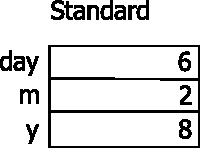
\includegraphics[height=4em]{chap2/fig1a}
		\caption{}
	\end{subfigure}
	~
	\begin{subfigure}[t]{0.3\textwidth}
		\centering
		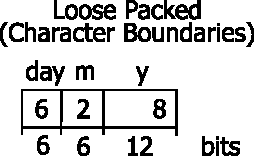
\includegraphics[height=4em]{chap2/fig1b}
		\caption{}
	\end{subfigure}
	~
	\begin{subfigure}[t]{0.3\textwidth}
		\centering
		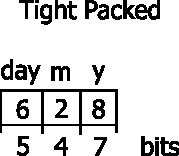
\includegraphics[height=4em]{chap2/fig1c}
		\caption{}
	\end{subfigure}
	\caption{日期 (7, March, 1908) 的表示}
\end{figure}

采用紧缩表示的第二种情况，是数据存储空间不足，无论是在主存还是外部辅助存储器中。不过，每当检查或更新数据时，都需要解开紧缩、再重新紧缩，这会使代码膨胀；必须注意，节省的数据存储空间不能被增加的代码空间抵消。

最小表示不常用于数据存储，因为它额外节省的空间很少（每个分量总是不到一位）；与通常的移位和掩码操作相比，每次访问分量都要乘除，增加的时间通常远远超过这点收益。不过，如果没有其他办法能把值放在合适的字边界之内，这种技术就可能有用，也可以与较常规的紧缩方法结合使用。此外，如果这个值只用于或主要用于给多维数组作索引，就应优先采用最小表示，因为这样能显著节省数组表示所需的空间（见第 \ref{sec:representation-6.2} 节）。

把 \textbf{with} 构造表示为机器码时，有时可以先计算所引用结构的地址，并把它保存在寄存器中；这样，访问分量的代码可能更短、更快。如果分量已经紧缩，可以在开始处理之前把它们解开，放入独立的字，以方便引用和更新；如果更新过这些分量，就必须在处理结束时重新紧缩，再存回结构中。在某些机器上，一次紧缩或解开整个结构，比逐个分量进行这些操作更经济。

\noindent
\textit{练习}
\nopagebreak

\noindent
给定变量

\quad today:date;

\noindent
编写程序，把紧接其后的日期赋给变量 tomorrow: date。采用紧密的紧缩表示，把这个程序翻译为你选择的机器码。分别使用非紧缩表示和最小表示重写程序。比较各自代码的长度，以及执行所需的时间。
\section[带判别标记的联合]{带判别标记的联合}

定义对象集合时，把一个集合定义为两个已知集合的并集，往往很有用。例如，在一副标准扑克牌中加入大小王后，扩展后的集合可以描述为标准牌集合与“百搭牌”joker 1、joker 2 所组成集合的并集。以这个集合的元素为取值的类型，可以声明为两种备选类型的联合：纸牌类型，以及有两个不同值的枚举类型：

\quad \textbf{type} pokercard $= ($normal:$(s$:suit; $r$:rank$)$,

\tabto{10.2em}wild:$($joker 1, joker 2$))$.

\noindent
pokercard 类型的每个值，要么对应一个有序对，其分量表示花色和点数；要么对应枚举类型中的一张王。

指定带判别标记的联合类型的常量时，必须指出它所表示的值来自哪一种备选类型。为此，要明确写出备选项的名称，例如：

\quad pokercard$($normal$($heart, Jack$))$

\noindent
表示来自第一种备选项的值，而

\quad pokercard$($wild$($joker 2$))$

\noindent
表示来自第二种备选项的值。一般而言，如果能从上下文推断类型，省略类型名会比较方便。

带判别标记的联合的第二个例子，可以来自维护一国所有汽车登记册的工作。汽车可以分为本国居民拥有的本地汽车，以及非居民临时带入境内的访客汽车。这两种情况下所需的信息很不相同。两种汽车的车牌号码和厂牌都被认为是有关信息。但对于本地汽车，还需要车主姓名，以及汽车首次登记在该车主名下的日期。对于访客汽车，这些信息无关紧要，只需要来源国名称的标准三字母缩写。因此，这两种备选汽车类型可以定义为：

\quad \textbf{type} local car = (make:manufacturer; regnumber:carnumber;

\tabto{9.4em} owner:person; first registration:date);

\quad \textbf{type} visitor car = (make:manufacturer; regnumber:carnumber;

\tabto{10.1em} origin:country);

现在就可以定义一个涵盖两类汽车的类型：

\quad \textbf{type} car $=$ (local:local car,

\tabto{7.4em} foreign:visitor car).

\noindent
不过，分别定义本地和外国汽车的结构并不方便；我们希望利用两者有若干相同分量这一事实。可以把共有分量移到两个备选项之前：

\quad \textbf{type} car $= ($make:manufacturer;

\tabto{7.5em}regnumber:carnumber;

\tabto{7.5em}$($local:$($owner:person;

\tabto{7.8em}first registration:date$)$,

\tabto{7.8em}foreign:$($origin:country$))$

\tabto{7.1em}$)$.

\noindent
每辆汽车都有 make 和 regnumber，但只有本地汽车才有 owner 和 first registration 日期；只有外国汽车才有 origin。

第三个例子是几何图形的定义。在某个应用中，图形可以分为矩形、三角形和圆：

\quad \textbf{type} figure $= ($position:point; rect:$R$, tri:$T$, circ:$C)$.

\noindent
各类图形的指定方式不同。对于矩形，要给出一条边的倾角，以及两条边的长度：

\quad \textbf{type} $R = ($inclination:angle; side1, side2:real$)$.

\noindent
三角形用一条边的倾角和长度，以及这条边与另外两条边形成的角来指定：

\quad \textbf{type} $T = ($inclination:angle; side:real; angle1, angle2:angle$)$.

\noindent
对于圆，只需用一个实数指定直径：

\quad \textbf{type} C $= ($diameter:real$)$.

把类型定义为若干其他类型的联合时，必须认识到：它的值应当被视为与任何组成类型的值完全不同。否则，就会立即违反“每个值只属于一个类型”的规则。因此，类型的联合必须与通常的集合并集概念明确区分。此外，对于联合类型的每个元素，都能确定它来自哪一种组成类型，即使同一种类型重复出现了多次。例如，玩纸牌接龙所用的两副牌，可以定义为两个牌组的联合：

\quad \textbf{type} patience card $=$ (red:cardface, blue:cardface).

\noindent
patience card 类型的每个值都明确标记着，它来自红色牌组还是蓝色牌组，即使现实中牌背颜色可能相同。这就解释了为什么把这种类型定义形式称为“带判别标记的联合”。由此可知，带判别标记的联合的基数，总等于各组成类型的基数之和。

\subsection{操纵}

带判别标记的联合的任何值，都附带一个\textit{判别标记}（tag）字段，指出它来自哪一种具体组成类型。赋值时，这个字段也要复制；相等测试时，要使两个值相等，其判别标记字段必须相同。

构造带判别标记的联合类型的值时，必须写出该值来源的备选类型名称：
\smallskip

\quad patience card$($red$($spade, Jack$))$.
\smallskip

\noindent
这样就会自动把值“red”赋给结果的判别标记字段。

某辆特定汽车可以表示为：
\smallskip

\quad car$($Ford, ``RUR157D'', local$($me, date$($1, Sept, 1968$)))$.
\smallskip

要访问并操作编码为带判别标记的联合的信息，需要把它转换回原来的类型。可以约定把该类型的标号当作选择函数使用，例如：

card1.wild \tabto*{8em} 的类型是 $($joker 1, joker 2$)$

car1.foreign \tabto*{8em} 的类型是 $($origin:country$)$

fig1.tri \tabto*{8em} 的类型是 $T$

\noindent
如果组成类型是笛卡尔积，就可以对所得值合法地使用它的选择函数；约定点运算符向左结合。

\quad card1.normal.$r$

\quad car1.local.owner

\quad fig1.circ.diameter

如果程序员试图把带判别标记的联合的值转换回一个\textit{并非}其来源的类型，就犯了严重的程序设计
错误，可能产生无意义的结果。这种错误只能通过运行时检查来发现：每当显式或隐式调用这种转换时，都检查判别标记字段。检查既费时，一旦失败又很不方便。因此，我们希望找到一种记法，保证这种错误绝不会在运行中的程序里发生；而且，只检查文本就能作出保证，无须知道程序运行时正在处理的值。如果有自动编译器，也可以由它提供这样的保证。

我们提出的记法，是笛卡尔积的 \textbf{with} 构造与分情况选择的 case 构造的结合。设联合类型的值 $sv$，需要根据它来自哪种备选类型，以几种不同方式之一进行处理。那么可以写：

\quad \textbf{with} $sv$ \textbf{do} $\{a1:S_1$

\tabto*{7.6em}$a2:S_2$,
\smallskip

\tabto*{8.85em}\vdots

\tabto*{7.6em}$an:S_n\}$;

\noindent
其中，每当 $sv$ 的判别标记字段值为 $a_i$ 时，就选择执行语句 $S_i$。在 $S_i$ 内，只要 $sv$ 的值保持不变，就可以安全地假定它来自对应的备选类型。因此，可以直接使用为该备选类型定义的分量选择函数来引用 $sv$ 的分量，就像前面为笛卡尔积介绍的简单 \textbf{with} 语句一样。

如果希望把联合类型看作有序的，最自然的顺序是：列表中较早备选项对应的所有值，都排在较晚备选项的任何值之前。

\noindent
\textit{练习}
\nopagebreak

\noindent
编写函数，计算按上述定义给出的图形的面积。

\subsection{表示}

表示带判别标记的联合的值时，首先需要把判别标记表示为从零到 $n - 1$ 的一个整数，其中 $n$ 是备选类型的个数。判别标记后面紧接着原类型的值的表示。与笛卡尔积一样，表示的紧缩程度可以选择。

在非紧缩表示中，判别标记占一个完整的字；联合类型的每个值所占空间，比最大备选类型的值多一个字。在紧缩表示中，这一额外开销可以缩减为几位。在最小表示中，把每个值在原类型中的最小表示，加上联合中所有排在它之前的类型的基数之和，就得到该值的表示。因此，来自第一种类型的值，例如 (diamond, four)，其表示值与原类型中的表示完全相同，即 16。但 joker 1 在原枚举类型中的表示值为零，需要再加上纸牌类型的基数。

在非紧缩、紧缩和紧密的紧缩表示之间选择时，所依据的考虑与笛卡尔积相同。不过，最小表示的运行速度代价要小得多，因为恢复原值只需减法，不需除法。

一般而言，不同备选类型的值占用的存储空间不同，因此必须为较短的值“补齐”填充，使各值长度相同，从而遵守初等数据类型占用固定存储量这一方便的规则。后面的章节将会说明，当值是某个更大结构的分量时，这种填充常常可以省去。

\begin{figure}[ht!]
	\centering
	\begin{subfigure}[b]{0.4\textwidth}
		\centering
		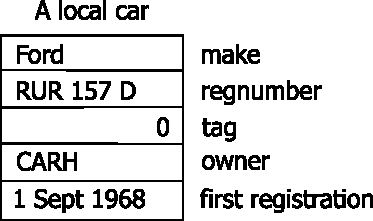
\includegraphics[height=6em]{chap2/fig2a}
	\end{subfigure}
	~
	\begin{subfigure}[b]{0.4\textwidth}
		\centering
		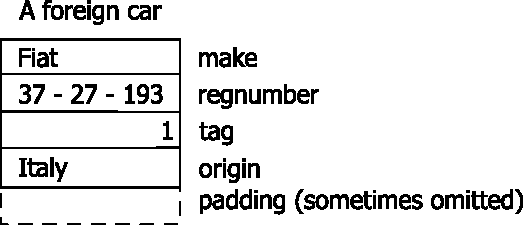
\includegraphics[height=6em]{chap2/fig2b}
	\end{subfigure}	
	\caption{汽车的表示}
\end{figure}

在当今程序设计实践中，联合的表示省略判别标记字段，是相当常见的做法。要正确操作这种表示，程序员必须根据其他因素“知道”该值应如何解释，因为无法从值本身查明。如果他的判断有误，无论运行时还是编译时检查，都无法发现。由于这类错误的效果取决于位模式表示的细节，所得结果无法用程序员正在使用的抽象概念来预测。因此，一般看来，应当把使用判别标记字段、采用可在编译时检查的分情况选择作为标准做法，只有特殊情况下才绕过它们。

\subsection{例子}

回到第 \ref{sec:example-3-3} 节的例子，即把语言文本分析为有意义的符号。我们希望严格地抽象定义这些符号究竟是什么。

\quad \textbf{type} symbol $=$

\tabto*{5.6em}$($realconst:real,

\tabto*{6em}integerconst:integer,

\tabto*{6em}identifier:ident,

\tabto*{6em}basic:delimiter$)$;

\noindent
其中，暂时不定义 ident 类型，并假定各个界符通过枚举定义。
\section[数组]{数组}
\label{sec:array}

对于许多程序员，数组是最熟悉的数据结构；在某些程序设计语言中，它还是唯一明确提供的结构。从抽象角度看，数组可以视为一个映射：从某个类型的定义域（下标范围），映射到一个可能属于不同类型的值域（数组的类型，或更准确地说，数组元素的类型）。

数学家通常用箭头指定映射的类型：

\quad $M:D\rightarrow R$;

\noindent
其中 $D$ 是定义域类型，$R$ 是值域类型。另一种程序员更熟悉的记法是：

\quad M:\textbf{array} $D$ \textbf{of} $R$.

\noindent
这种记法更能体现数据的表示方式，而数学记法强调的是结构的抽象性质，与具体表示无关。

把映射类型的某个具体值 $M$ 应用于定义域类型的值 $x$ 时，它指定值域类型中的唯一一个元素，称为 $M$ 在 $x$ 处的值，可以用圆括号或方括号写成：

\quad $M(x)$ 或 $M[x]$。

\noindent
映射也叫函数。这里采用“映射”一词，是为了把这种数据结构与一段程序区分开：后者确实根据定义域中的参数，计算出值域中的一个值。区别的本质在于，映射 $M$ 并非通过给出计算方法来指定，而是通过明确列出定义域中每个可能值 $x$ 所对应的 $M(x)$ 来指定。因此，数组只能用于在有限个点上定义的函数，而计算函数的定义域可以是无限的。

有限映射的一个例子是 monthtable，它为一年中的每个月指定该月的天数：

\quad \textbf{type} monthtable $=$ \textbf{array} month \textbf{of} $28\,.\,.\,31$.

\noindent
定义域是 month 类型，值域类型由 28 到 31（包含端点）的整数构成。要指定这个类型的一个典型值，只需让 $x$ 遍历定义域，并列出各个 $M(x)$ 的值。因此，如果 $M$:monthtable 被指定为：

\quad monthtable$($Jan:31, Feb:28, March:31, April:30,

\quad May:31, June:30, July:31, Aug:31,

\quad Sept:30, Oct:31, Nov:30, Dec:31$)$

\noindent
那么 $M[\text{Jan}] = 31,\, M[\text{Feb}] = 28$，依此类推。

数组提供了一种表示一副牌中某种具体排列的方法，因为每种排列都可以视为一个映射，为牌组中五十二个可能位置各自指出占据该位置的纸牌。因此，每种可能的排列都可以视为以下映射类型的一个值：

\quad \textbf{type} cardpack = \textbf{array} $1\,.\,.\,52$ \textbf{of} cardface.

\noindent
当然，并非该类型的所有值都表示实际的牌组，因为没有任何条件阻止某个值把两个不同位置映射到同一张牌，而现实中这是不可能的。

元素属于笛卡尔积类型的数组，有时称为\textit{表}。

数组的第三个例子，表示普通穿孔卡上字符穿孔的一切可能配置。它可以看作映射 $M$，把每个列号映射为一个字符，即该列穿孔所表示的字符。

\quad \textbf{type} punchcard = \textbf{array} $1\,.\,.\,80$ \textbf{of} character.

\noindent
卡片上任何可能的穿孔文本，都可以视为 punchcard 类型的一个值。

第四个例子用数组表示阴极射线管显示设备上一页内容的某个可能值。假定它有 40 行，每行有 27 个字符位置。把映射的定义域指定为所有可能行号与每行所有可能字符位置的笛卡尔积，就可以得到二维效果。写法如下：

\quad \textbf{type} spot $= ($row:$1\,.\,.\,40$; column:$1\,.\,.\,27)$;

\quad \textbf{type} display page $=$ \textbf{array} spot \textbf{of} character.

处理多维数组的另一种方法，是把它看作由行组成的数组，而每一行又是字符数组：

\quad \textbf{type} display page $=$ \textbf{array} $1\,.\,.\,40$ \textbf{of} row;

\quad \textbf{type} row $=$ \textbf{array} $1\,.\,.\,27$ \textbf{of} character.

\noindent
如果要逐行处理而不逐列处理，这种抽象结构更合适。

数组类型的基数，是值域类型的基数的若干次幂，指数为定义域类型的基数，即：

\quad cardinality$(D \rightarrow R) =$ cardinality$(R)^{\text{cardinality}(D)}$

\noindent
可以通过考察完整指定一个数组类型的值需要作多少次选择，来证明这一点。对于定义域的每个值，都要从值域类型的 cardinality$(R)$ 个可能值中选出一个。每个数组元素都要独立地作一次这样的选择，也就是总共选择 cardinality$(D)$ 次。

\subsection{操纵}

把定义域的所有值都映射到值域中同一个值的映射，称为常值映射。数组的一种自然构造函数，接受任意值域值作为参数，产生一个常值数组，其中所有元素都等于给定的值域值。直接用类型名来表示这个构造函数会很方便，例如：

\quad $M = \text{monthtable}(31)$

\noindent
是一个数组，对于所有月份 m，都有 $M[m] = 31$。

\quad card pack$($cardface$($heart, King$))$

\noindent
显然是一副魔术师用的牌。

数组的基本构造操作，是为数组中某个特定元素定义一个新值。如果 $x$ 是数组类型 $T$ 的值，$d$ 是其定义域类型的值，$r$ 是其值域类型的值，那么写：

\quad $T(x, d:r)$

\noindent
表示 $T$ 类型的一个值，它除把 $d$ 映射到 $r$ 之外，在所有方面都与 $x$ 相同。如果能从上下文推断出 $T$，就可以省略它。类似地，常值数组 $T(x)$ 可以写为 all $(x)$。

数组的基本选择运算符是下标运算。它实质上是一个二元操作，作用于数组和一个定义域类型的值，产生对应的值域类型的值。

改变数组值最常见、最高效的方法，是选择性地更新某个分量。采用通常的记法，把带下标的数组变量放在赋值号左边，就能实现这一点：

\quad $a[d]\coloneq r.$

\noindent
它与下式意义相同：

\quad $a\coloneq T(a, d:r).$

\noindent
注意，从抽象角度看，是把一个新值赋给整个数组。

数组类型通常被视为无序的；但某些情况下，尤其是字符数组，我们希望定义一种与通常字典序一致的顺序。只有定义域类型和值域类型都有序时，才可能这样做。这时，两个数组的次序，由它们最小的不同下标处的元素次序决定。因此：

\quad ``BACK'' $<$ ``BANK''

\noindent
因为第三个字母是两者最先不同的地方，而且

\quad ``$C$'' $<$ ``$N$''

指定数组值的一种方便方法，是使用仿照 for 语句构造的\textit{for 表达式}：

\quad \textbf{for} $i:D$ \textbf{take} $E$

\noindent
其中，$E$ 是包含变量 $i$、产生值域类型值的表达式。当 $i$ 遍历定义域类型 $D$ 时，对 $E$ 求值，就得到相应数组元素的值。

如果数组的值域类型定义了某些操作，自然可以把这些操作推广到数组类型。例如，如果 $A$ 和 $B$ 是具有相同定义域的实数数组，就可以自然地写：

\quad $A + B,$ $A - B$,

表示定义域相同的数组，其元素分别是 $A$、$B$ 对应元素值的和与差。但程序员必须始终意识到，数组很大时，这些操作的成本可能很高；在从抽象程序推进到更具体程序的过程中，应当设法消除这些操作。

\subsection{表示}
\label{sec:representation-6.2}

大多数程序员都熟悉数组在计算机存储器中的表示。最常见的是非紧缩表示，为每个数组元素分配一个或多个完整的字。这种情况下，各元素的计算机地址可以简单地计算出来：先把下标值转换为最小表示，再乘以每个元素占用的字数，最后把结果加到数组第一个元素的地址上。利用计算机通常的按字选择机制，就可以访问和更新这个值，而不影响其他数组元素。

另一种表示把元素紧缩在字边界之内，使每个元素只占一个字内固定数量的位，虽然整个数组可能跨越多个字。以 monthtable 为例，每个元素只有四种取值，从 28 到 31；因此，在最小表示中只需两位就能容纳，整个数组也就可以容纳在二十四个连续的位中。

数组按这种方式紧缩时，选择带下标变量的值就复杂得多。为了选出正确的字，必须把下标的最小表示除以每个字包含的元素个数。把商加到数组第一个字的地址上，随后访问该字。把余数乘以每个元素的位数，用结果作为 $\text{shift-count}_2$，把所需值移到字内的标准位置。然后，可以用掩码去掉相邻数组元素中不需要的值。对紧缩数组元素进行选择性更新更加费事，因为必须把新值插到字内的正确位置，同时不改变相邻元素的值。如果每个字的元素个数恰好是二的幂，两种操作的效率都可以略有提高：下标的整数除法，可以用移位求商、用掩码求余数来替代。在某些机器上，把每个元素存储在单个字符位置，还能进一步提高效率。

数组的最小表示类似于笛卡尔积的最小表示，不过，每个元素值所乘的因子，等于值域类型基数的下标值次幂。除非值域类型的基数恰好是二的幂，否则选择或更新以最小表示存储的数组元素，比上面描述的过程还要费事。如果数组跨越多个普通计算机字，其代价就高得难以接受。因此，数组的最小表示主要只有理论意义。

\begin{figure}[h]
	\centering
	\begin{subfigure}[b]{0.3\textwidth}
		\centering
		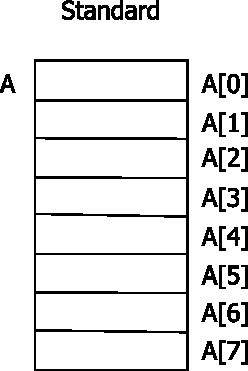
\includegraphics[height=10em]{chap2/fig3a}
		\caption{}
	\end{subfigure}	
	\begin{subfigure}[b]{0.3\textwidth}
		\centering
		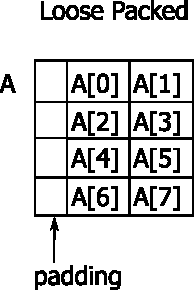
\includegraphics[height=8em]{chap2/fig3b}
		\caption{}
	\end{subfigure}	
	\begin{subfigure}[b]{0.3\textwidth}
		\centering
		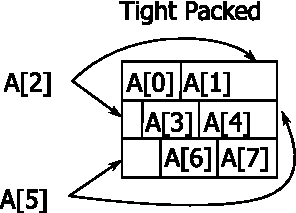
\includegraphics[height=5.5em]{chap2/fig3c}
		\caption{}
	\end{subfigure}%
	\caption{$A:\text{\textbf{array} } 0\,.\,.\,7 \text{ \textbf{of} } T$ 的表示}
\end{figure}

有限映射的定义域本身是数据结构时，例如笛卡尔积，通常用最小表示来表示定义域，以免分配用不到的存储空间。例如，display page 的定义域，是整数范围 1 到 40 与 1 到 27 的笛卡尔积。采用最小表示，就得到从 0 到 $40 \times 27 - 1 = 1079$ 的整数范围。因此，分配 1080 个连续的字来保存数组元素的值。要访问给定行和字符位置处的元素，首先必须按第 \ref{sec:representation-4-2} 节介绍的方法，为下标构造最小表示。

多维数组的另一种表示方法，有时称为代码字方法或描述符方法，不过我们把它称为“树形表示”。其要点是分配一个一维\textit{基}数组，每个元素对应原数组的一行，并在其中存放一段连续存储区域的地址，该区域保存那一行的值。各行之间不必连续。这样，访问或更新元素时，就不必计算下标的最小表示。只需把行号加到树的基数组第一个元素的地址上，就能访问所需行第一个元素的地址；再把下一个下标值加到这个地址上，就得到所需元素的地址。

\begin{figure}[h]
	\centering
	\begin{subfigure}[b]{0.35\textwidth}
		\centering
		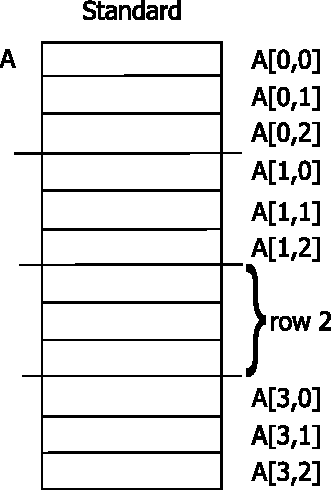
\includegraphics[height=12em]{chap2/fig4a}
		\caption{}
	\end{subfigure}	
	\begin{subfigure}[b]{0.6\textwidth}
		\centering
		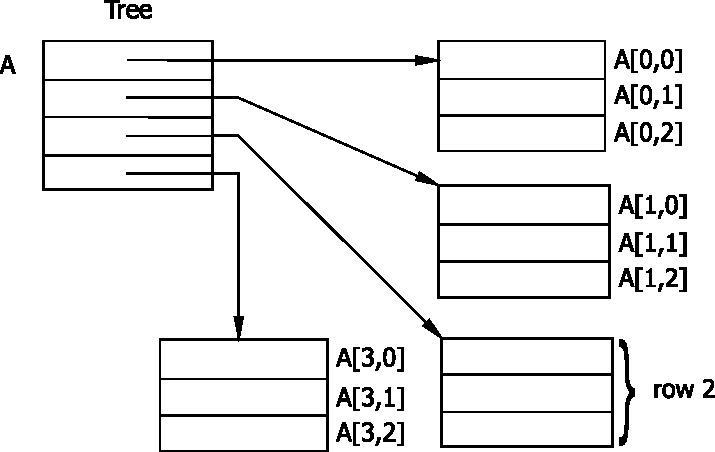
\includegraphics[height=10.5em]{chap2/fig4b}
		\caption{}
	\end{subfigure}	
	\caption{二维数组的表示}
\end{figure}

在数组的非紧缩表示与紧缩表示之间选择，依据与笛卡尔积类似。如果需要快速访问和更新，就采用非紧缩表示；如果值域类型本来就适合放在计算机字边界内，例如元素是浮点数，这也是显然合适的选择。如果元素远短于一个字，并且存储空间不足，或数组的复制、比较比下标访问和选择性更新更频繁，就建议采用紧缩表示。紧缩数组一个特别常见的用途，是表示程序设计语言中的标识符。为了效率，可以把长到标准数组放不下的标识符截断，把过短的标识符用空白补齐。

多维数组表示方式的选择，依据则很不一样。标准表示更加节省存储空间，按行、按列或同时按行列遍历数组元素时，效率都很好。此外，如果数组必须整体在主存和辅助存储器之间传送，它也更方便。不过，在乘法较慢的机器上，采用树形表示更快，代价是接受保存地址数组所需的额外空间；只要每行不太短，这点空间并不大。如果每行只有两个字，数据存储就会多出百分之五十的开销。

选择树形表示还可能有几个其他理由：

\begin{enumerate}[wide, nosep, label=(\arabic*)]
	\item 在某些普遍采用动态存储分配的计算环境中，可能很难获得大块连续区域。这时，可以把大型二维数组拆成若干较短的行，方便地安排存储。

	\item 可以建立一种机制：处理某些行时，把其他行保存在辅助存储器中；当某一行不在主存中时，基数组中该行的主存地址由其辅助存储地址替代。这样，有望处理无法与处理程序一起完整放入主存的大数组。不过，必须仔细考察这种操作的成本，确保辅助存储传送次数可以接受。

	\item 在某些应用中，已知几个矩阵共享相同的行。树形表示可以只保存这种共享行的一份副本，复制它的地址，而不复制完整的值。但这种情况下，不能对共享行进行选择性更新。

	\item 即使对于一维数组，如果各元素的大小变化很大，也建议采用树形表示；对于多维数组，如果各行长度变化很大，同样建议采用它。
\end{enumerate}

\noindent
\textit{练习}
\nopagebreak

\noindent
某输入设备的字符集只有三十个字符，用枚举定义，其中包括 space、newline 和 newpage。可以调用过程

\quad read next character.

\noindent
从输入设备一次读入一个字符，放入缓冲区。应当逐行把这些字符组合到数组

\quad page:display page,

\noindent
中；收到 newpage 字符时，用指令

\quad outpage.

\noindent
把它输出到显示设备。显示设备\textit{不}识别 newline 或 newpage 字符，因此必须用空格填满行尾和页尾的剩余部分。

用合适的语言编写程序完成这一操作，并为 display page 选用不同表示，例如：

\quad 非紧缩表示

\quad 较松的紧缩表示

\quad 紧密的紧缩表示

\quad 间接表示。

\noindent
使用不同表示重写程序。比较不同表示涉及的代码和数据长度，以及运行速度。

编写相应程序，从显示设备读取一页，输出各个字符；注意尽可能去掉每行末尾多余的空格，以及每页末尾的空白行。
\section[幂集]{幂集}

给定集合的幂集，定义为该集合所有子集组成的集合；幂集类型的值则是集合，其元素从另一个类型中选取，这个类型称为幂集的\textit{基}类型。例如，原色已通过枚举定义为 red、yellow 和 blue。其他主要颜色由两种或三种原色混合而成：橙色是红色与黄色的混合，棕色是三种原色的混合。因此，每种主要颜色（包括原色）都可以用能混合出它的原色子集来指定。例如，橙色可以看作只有 red 和 yellow 两个元素的集合。用枚举定义集合的传统记法，可以写成 $\{$red, yellow$\}$。纯红色可以看作只有原色 red 一个元素的集合，即 $\{$red$\}$。这样，就能表示七种主要颜色：红、橙、黄、绿、蓝、紫和棕。没有任何原色时（即空集），可以把它看作表示没有颜色，例如白色。以这些颜色为取值的类型，可以声明为 primary color 类型的幂集：

\quad \textbf{type} color $=$ \textbf{powerset} primary color.

第二个例子来自表示电梯请求按钮状态所需的数据结构。floor 类型的简单变量（见第 \ref{sec:unstructured-data-types} 节），能够指出电梯的某一个停靠楼层。但如果要记录电梯内部整块按钮面板的状态，就需要用楼内所有可能楼层的一个子集来表示，即请求按钮已被按下的那些楼层组成的子集。因此，可以把 liftcall 类型定义为 floor 类型的幂集：

\quad \textbf{type} liftcall $=$ \textbf{powerset} floor.

第三个例子来自某种纸牌游戏，例如扑克或桥牌中的一手牌。一手牌是纸牌集合中没有重复元素的子集，因此适合用以下幂集类型中的一个值表示：

\quad \textbf{type} hand $=$ \textbf{powerset} cardface;

\noindent
这个类型涵盖至多五十二张牌的所有手牌，即使某种具体游戏会规定标准手牌张数，或把上限设为小于五十二的数。

最后一个例子表示计算机外部设备的状态，例如纸带读入机。尝试输入字符时，可能出现若干异常情况：

\begin{enumerate}[wide, nosep, label=(\arabic*)]
	\item 操作员把设备切换到“手动”。
	\item 没有装入纸带。
	\item 最近读入的字符发生奇偶校验错误。
	\item 最近读入字符时检测到纸带偏斜。
\end{enumerate}

\noindent
这些情况可以定义为一个枚举类型：

\quad \textbf{type} exception $= ($manual, unloaded, parity, skew$)$; 

\noindent
由于可能同时检测到其中几种情况，读入机的状态可以指定为某个幂集类型的值：

\quad \textbf{type} statusword $=$ \textbf{powerset} exception.

幂集类型的基数等于二的若干次幂，指数为基类型的基数，即：

\quad cardinality$(\text{\textbf{powerset} } D) = 2^{\text{cardinality} (D)}$

可以通过考察完整指定该类型的一个值需要作多少次决定，来证明这一点。对于基类型的每个值，都有两种选择：它在集合中，或不在集合中。这样的决定可以独立地作 cardinality$(D)$ 次。

\subsection{操纵}

集合的基本构造操作，是从定义域类型中取得若干值，把它们转换为一个恰好以这些值为元素的集合。与笛卡尔积一样，类型名用作转换函数；但对于集合，参数个数可以变化，从零个开始。例如：

\quad primary color$($red, yellow$)$ \tabto*{14em} 即橙色

\quad liftcall$($ground$)$ \tabto*{14em} 即只按下了一个按钮

\quad statusword$()$ \tabto*{14em} 即没有异常情况。

\noindent
后两个例子分别说明了\textit{单元素集合}（必须与其唯一元素明确区分）和不含任何元素的\textit{空集}的概念。如果在这种构造中省略类型名，就应按通常做法使用花括号，而不是圆括号。

与空集相对的是全集，它包含基类型中的所有值。可以记为：

\quad $T$.all.

\noindent
不过，只有基类型有限时，这个全集才作为可存储的数据值存在。

数学家和逻辑学家对集合的基本操作都很熟悉。

\begin{enumerate}[wide, nosep, label=(\arabic*)]
	\item 元素归属测试：如果 $x$ 在集合 $s$ 中，布尔表达式“$x$ \textbf{in} $s$”的值为 true，否则为 false。
	\item 相等：两个集合相等，当且仅当它们具有相同的元素。
	\item 交：$s_1 \wedge s_2$ 恰好包含同时在 $s_1$ 和 $s_2$ 中的那些值。
	\item 并：$s_1 \vee s_2$ 恰好包含在 $s_1$ 或 $s_2$ 中，或同时在两者中的那些值。
	\item 相对补集：$s_1 - s_2$ 恰好包含 $s_1$ 中不在 $s_2$ 里的那些元素。
	\item 包含关系测试：只要 $s_1$ 的所有元素也是 $s_2$ 的元素，$s_1 \subset s_2$ 的值就为 true，否则为 false。
	\item 集合的大小说明它有多少个元素。

	如果一个集合的定义域类型定义了某些运算符，构造相应的集合操作往往很有用。特别是，如果定义域类型有序，就可以使用以下运算符：

	\item $\min(s)$ 是 $s$ 的最小元素；$s$ 为空时未定义。
	\item $s \text{ \textbf{down} } n$ 是一个集合，恰好包含那些第 n 个后继在 $s$ 中的值。
	\item $s \text{ \textbf{up} } n$ 是一个集合，恰好包含那些第 $n$ 个前驱在 $s$ 中的值。
	\item Range$(a,\ b)$ 在 $a \leqslant b$ 时是包含 a、succ$(a), \dots, b$ 的集合，否则为空。
\end{enumerate}

集合最有用的选择性更新操作是：

\noindent
$x:\vee\ y$; \tabto*{5em} 把集合 $y$ 并入 $x$

\noindent
$x:\vee\ T(a)$ \tabto*{5em} 把元素 $a$ 加入 $x$

\noindent
$x:\wedge\ y$; \tabto*{5em} 从 $x$ 中删除所有不属于 $y$ 的元素

\noindent
$x:-\ y$ \tabto*{5em} 从 $x$ 中删除所有也属于 $y$ 的元素

\noindent
\hangindent=3.2\parindent$x:\text{\textbf{down} }n$ \tabto*{5em} 把 $x$ 的每个元素减去 $n$，不能这样做的元素则删除

\noindent
\hangindent=3.2\parindent$x:\text{\textbf{up} } n$ \tabto*{5em} 把 $x$ 的每个元素加上 $n$，不能这样做的元素则删除

\noindent
有时，从 $x$ 中选出一个元素，并同时把它从 $x$ 中移除，也很有用。这个操作可以记为：

\quad $a$ \textbf{from} $x$.

\noindent
如果 $x$ 的定义域类型有序，自然应选取 $x$ 的最小元素；否则应把选择视为任意的。

常常可以用某个条件 $B$ 来定义集合的值：定义域类型中恰好满足 $B$ 的那些值，就是所需集合的元素。可以记为：

\quad $\{i:D \mid B\}$

\noindent
其中 \tabto*{4em} $i$ 是类型 $D$ 的变量，视为 $B$ 的局部变量，

\noindent
而 \tabto*{4em} $B$ 是一个布尔表达式，通常包含并依赖于 $i$。

\noindent
要使这个表达式表示幂集类型的一个值，$D$ 的基数必须有限，而且 $B$ 必须对该类型的所有值都有定义。

最后，经常需要对某个集合的每个元素进行某种操作，也就是执行一个循环，让计数变量依次取到集合中的所有值。合适的表达记法是：

\quad \textbf{for} $x$ \textbf{in} $s$ \textbf{do} \dots

\noindent
如果 $s$ 的基类型有序，规定从最小元素开始，按自然顺序选取各元素，是合理的。对于无序的基类型，程序员不关心按什么顺序选取元素，因此保留选择最有利于效率的顺序的余地。

\subsection{表示}

为幂集选择计算机表示时，希望所有基本操作都能简单地用单条机器码指令执行，同时尽量减少存储占用。对于大多数数据结构存储方法，这两个目标存在根本冲突，因此程序员必须在不同表示方法之间作出选择；但对于幂集，只要基类型不太大，两个目标就能完全兼顾。

建议的表示方法，是在存储器中分配与集合潜在元素个数相同数量的位。基类型的每个值都对应一个位；如果它确实属于集合，这个位为一，否则为零。例如，color 类型的每个值都能用三位表示；最高有效位对应原色 red，最低有效位对应 blue。因此，橙色表示为 110，红色表示为 100。大小为 $n$ 的每个集合，都表示为一个恰好在对应位置上有 $n$ 个一的位模式。因此，空集用全零位模式表示。

另一个例子是 hand 类型，它的表示需要五十二位，每一位对应 cardface 类型的一个值。这里，最好对基类型采用最小表示，以免位模式表示中留下不用的空隙。

由于幂集类型的值的个数总是二的整数次幂，对于基类型较小的幂集，在二进制计算机上不可能有比位模式表示更节省存储空间的方法。接下来还要说明，幂集类型上的操作也能高效执行。

\begin{enumerate}[wide, nosep, label=(\arabic*)]
	\item 要得到以 $x$ 为唯一元素的集合，可以在符号位位置装入一个 1，再向右移动 $x$ 位。在移位较慢的计算机上，可以用查表达到同样效果。用分量构造集合，可以把相应的所有单元素集合作逻辑并。

	\item 元素归属测试 $x$ \textbf{in} $s$，可以把 $s$ 向高位方向移动 $x$ 位，再检查最高有效位：1 代表 \textbf{true}，0 代表 \textbf{false}。

	\item 二进制计算机常常提供单条指令，执行逻辑交、并和取补。

	\item 有时可以用内置的机器码指令，统计一个字中值为 1 的位数，从而得到集合的大小。否则，可以反复执行规格化，每次用掩码清除紧邻符号位的那个位，来确定集合的大小。第三种办法是把位模式拆成若干小块，对每块查表，再把结果相加。

	\item \textbf{up} 和 \textbf{down} 操作显然可以用右移或左移完成。

	\item 可以用规格化指令高效找到集合的 min；这条指令自动计算，把第一个为一的位移到紧邻符号位的位置，需要移动多少位。

	\item for 语句也可以利用规格化高效实现，每遇到一个为一的位，就用掩码把它清除。

	\item range 操作可以用两次移位完成，第一次移位会重新补入符号位。	
\end{enumerate}

因此，只要定义域类型的基数，不大于计算机中可施加逻辑和移位操作的最大字的位数，所有这些操作都能高效执行。如果占用空间明显超过一个这样的字，使用选择性更新操作通常比使用一般的、产生结果值的运算符更划算。此外，size 和 min 这类操作可能变得相当低效。此时，往往可以把这些值与集合一起冗余保存，每当集合更新就同步维护，而不在每次需要时重新计算。

如果已知基类型的基数很大（甚至可能无限），而典型集合的大小相对很小，那么位模式表示就完全失去了吸引力，因为存储和操作大片零已经不划算。这种稀疏集合的处理留到第 \ref{sec:sparse-data-structures} 节再讨论。

\subsection{例子}

\noindent
\textit{问题}：编写程序，构造集合

\quad primes:\textbf{powerset} $2\,.\,.\,N$;

\noindent
使其包含基类型中的所有素数。

\noindent
采用埃拉托色尼筛法，避免所有乘法和除法。

埃拉托色尼的方法，是先把所有数放入“筛子”，然后重复以下步骤，直到筛子为空：

\noindent
选出并移除筛子中剩下的最小数（它必然是素数），然后逐步遍历筛子，移除这个数的所有倍数。

程序很容易写出：

\noindent
\textbf{begin} $n$, next:$2\,.\,.\,N$; sieve:\textbf{powerset} $2\,.\,.\,N$;

\noindent
\quad sieve $\coloneq$ range$(2, N)$;

\noindent
\quad primes $\coloneq \{\}$;

\noindent
\quad \textbf{while} sieve $\neq$ empty \textbf{do}

\noindent
\quad \quad \textbf{begin} next $\coloneq$ min$($sieve$)$;

\noindent
\quad \quad \quad primes: $\vee\ \{$next$\}$;

\noindent
\quad \quad \quad \textbf{for} $n\coloneq$ next \textbf{step} next \textbf{until} $N$ \textbf{do}

\noindent
\quad \quad \quad \quad sieve:$-\ \{n\}$

\noindent
\quad \quad \textbf{end}

\noindent
\textbf{end} primefinder.

但如果 $N$ 很大，例如在 $10\,000$ 的数量级，这个程序直接执行时就无法达到可以接受的效率。解决办法是把它作为算法的抽象模型，改写为更高效的形式，只使用不超过计算机字长的集合上的操作。因此，需要声明一个字数组来表示这两个集合，并假定“wordlength”是一个环境查询值，给出一个字包含的位数：

\quad primes, sieve:\textbf{array} $0\,.\,.\,W$ \textbf{of powerset} $0\,.\,.\,\text{wordlength} - 1$

\noindent
其中 $W = (N + 1) \div \text{wordlength} + 1$。

\noindent
这意味着两个集合可能略大于 $N$，但为方便起见，接受这种无害的扩展。

为了访问这些集合中的一个位，必须同时知道字号和位号。由于不想用除法来求它们，我们把计数变量 $n$ 和 next 表示为笛卡尔积：

\quad $n$, next:$(w,\ b$:integer$)$;

\noindent
其中 $w$ 表示字号，$b$ 表示位号。

现在不妨先重新编码最内层循环，检查这种表示的效率。

\quad \textbf{for} $n\coloneq$ next \textbf{step} next \textbf{until} $N$ \textbf{do} sieve:$-\ \{n\}$;

\noindent
改写为：

\quad $n\coloneq$ next;

\quad \textbf{while} $n.w \leqslant W$ \textbf{do}

\quad \quad \textbf{begin} sieve$[n.w]$:$-\ \{n.b\}$;

\quad \quad \quad $n.b\coloneq n.b + \text{next}.b$;

\quad \quad \quad $n.w\coloneq n.w + \text{next}.w;$

\quad \quad \quad \textbf{if} $n.b \geqslant$ wordlength \textbf{then begin} $n.w \coloneq n.w + 1$;

\quad \quad \quad \quad $n.b \coloneq n.b - \text{wordlength}$

\quad \quad \quad \textbf{end}

\quad \quad \textbf{end}

\noindent
看来这样的效率可以接受，于是继续编码外层循环的其他操作，从最困难的开始：

\quad next $\coloneq$ min$($sieve$)$;

\noindent
这里，不希望每次都从 sieve 集合的起点开始搜索最小值，因为过程接近结束时，这样会扫描许多空字。因此，我们利用这一事实：next 的新值必定大于旧值。

搜索分两步：先找一个非空字，再找其中第一个为一的位。但如果搜索字时到达数组末尾，整个程序就完成了。

\quad \textbf{while} sieve$[\text{next}.w] = \{\}$ \textbf{do} $\{\text{next}.w \coloneq \text{next}.w +1$;

\quad \quad \textbf{if} next.$w > W$ \textbf{then exit} primefinder$\}$;

\quad \quad next.$b\coloneq$ min$(\text{sieve}[\text{next}.w])$;

其他操作都很简单。由于外层循环用 exit 终止，就不必再单独测试 while 条件；语句

\quad primes:$\vee\ \{$next$\}$;

\noindent
可以编码为：

\quad primes$[\text{next}.w]$:$\vee\ \{\text{next}.b\}$.

包含初始化的整个程序如下：

\quad primes, sieve: \textbf{array} $0\,.\,.\,W$ \textbf{of powerset} $0\,.\,.\,\text{wordlength} - 1$;

\quad \textbf{begin} primefinder;

\quad \quad $n$, next:$(w, b$:integer$)$;

\quad \quad \textbf{for} $t$:$0\,.\,.\,W$ \textbf{do begin} primes$[t] \coloneq \{\}$;

\quad \quad \quad sieve$[t] \coloneq$ range $(0\,.\,.\, \text{wordlength} - 1)$

\quad \quad \textbf{end};

\quad \quad sieve$[0]$:$-\ \{0, 1\}$;

\quad \quad next.$w\coloneq 0$;

\quad \quad \textbf{while} true \textbf{do}

\quad \quad \quad \textbf{begin while} sieve$[\text{next}.w] = \{\}$ \textbf{do}

\quad \quad \quad \quad \textbf{begin} next.$w\coloneq$ next.$w + 1$;

\quad \quad \quad \quad \quad \textbf{if} next.$w > W$ \textbf{then exit} primefinder

\quad \quad \quad \quad \textbf{end};

\quad \quad \quad \quad next.$b\coloneq$ min$($sieve$[\text{next}.w])$;

\quad \quad \quad \quad primes$[\text{next}.w]$: $\vee\ \{\text{next}.b\}$;

\quad \quad \quad \quad $n\coloneq$ next;

\quad \quad \quad \quad \textbf{while} $n.w \leqslant W$ \textbf{do}

\quad \quad \quad \quad \quad \textbf{begin} sieve$[n.w]$:$-\ \{n.b\}$;

\quad \quad \quad \quad \quad \quad $n.b\coloneq n.b + \text{next}.b$;

\quad \quad \quad \quad \quad \quad $n.w\coloneq n. w + \text{next}.w$;

\quad \quad \quad \quad \quad \quad \textbf{if} $n.b \geqslant$ wordlength \textbf{then}

\quad \quad \quad \quad \quad \quad \textbf{begin} $n.w\coloneq n.w + 1$;

\quad \quad \quad \quad \quad \quad \quad $n.b\coloneq n.b - \text{wordlength}$

\quad \quad \quad \quad \quad \quad \textbf{end}

\quad \quad \quad \quad \quad \textbf{end}

\quad \quad \quad \textbf{end}

\quad \textbf{end} primefinder

这个程序的一个特点，是使用环境查询 word length，充分发挥机器所能达到的效率，同时又完全独立于机器。即使在字长差别很大的机器上，程序也不仅能运行，而且能高效运行。

但这个程序最值得关注的特点，是它与前一版本的关系。从抽象角度看，两者表达的是同一个算法；改变的只是计算机上的数据表示方式。最初的设计充当了框架或范式，第二个版本更复杂的编码就是据此组织的。分两个阶段进行设计，简化了这样一项任务：确保最终程序的每个部分都能与其他部分成功配合。

\noindent
\textit{练习}
\nopagebreak

\noindent
使用只表示奇数的集合重写程序。（提示：先重写更抽象的程序。）
\section[序列]{序列}

前面的章节讨论了初等数据结构。它们在实际程序设计中非常重要，在现代数字计算机上表示和操纵时，也几乎不造成困难。此外，它们为构造一切更高级的结构提供了不可缺少的基础。

初等结构化类型与高级结构类型最重要的区别在于：只要组成类型的基数有限，前者的基数就严格有限。有限集合与无限集合的区别，具有深刻的数学意义，也给表示和操纵方法带来许多影响。

\begin{enumerate}[wide, nosep, label=(\arabic*)]
	\item 高级结构类型的潜在值可能有无限多个，因此，保存某个值所需分配的存储量，无法仅凭声明来确定。通常只有程序实际运行时才能确定，而且在许多情况下，它会在执行过程中变化。对于初等结构，不同潜在值的个数有限，保存任意值所需的最大存储量是固定的，可以由声明形式确定。

	\item 结构化值的大小相当大时，分别更新结构的各个分量，比给整个结构赋一个全新值更高效。即使对于初等类型，有时也发现选择性更新更高效，尤其是非紧缩表示的笛卡尔积和数组。对于高级数据结构，选择性更新的效率优势通常更加明显。

	\item 大小动态变化的高级数据结构，需要某种动态存储分配和释放机制。所需的存储单元通常用指针连接起来，指针有时也称为引用或地址；释放则通过显式编程操作，或某种通用垃圾回收来完成。动态存储分配和指针的使用，显著增加了处理复杂性；当数据必须在计算机主存与辅助存储器之间传送时，问题尤其严重。对于初等数据结构，这类问题完全可以不出现。

	\item 为高级数据结构选择合适表示，往往比为初等结构选择表示困难得多。各种基本操作的效率强烈依赖表示选择，因此，要作出合理选择，就需要知道这些操作的相对调用频率。结构的一部分或全部保存在辅助存储器上时，这一点尤其重要；此时，表示的选择还应考虑硬件设备的特性，即旋转介质上的磁道和柱面排列，以及磁头移动时间和旋转延迟。对于初等结构，在大多数表示中，各基本操作的效率大致相当。
\end{enumerate}

由此可见，高级结构与初等结构差别十分明显，高级结构带来的问题也大得多。这说明，对于实际程序员，明智的做法是尽可能只使用初等结构，只有应用本身迫使他这样做时，才使用高级结构。

高级数据结构中，第一个也是最熟悉的例子是序列。它仅仅被看作某个给定类型的任意多个项按顺序组成的结构。“序列”一词意在涵盖磁带、磁盘、磁鼓或主存中的序列。主存中的序列，有时称为流、表、串、栈、双端队列、队列，甚至集合。文件（或顺序文件）一词，常用于保存在辅助存储器中的序列。序列概念是一种抽象，所有这些结构都可以视为它的不同表示。

序列的第一个例子是串，ALGOL 和 SNOBOL 程序员对它很熟悉。串由任意长度的字符序列构成，因此可以定义为：

\quad \textbf{type} string $=$ \textbf{sequence} character.

第二个例子来自数据处理应用，即维护一个汽车数据文件。文件中的每个项（有时称为记录）表示一辆汽车，因此属于 car 类型；前面已经给出了 car 类型的一种可能定义：

\quad \textbf{type} car file $=$ \textbf{sequence} car.

第三个例子给出处理一副牌的另一种方法。它可以看作一个纸牌序列，其长度可能随发牌而变化：

\quad \textbf{type} deck $=$ \textbf{sequence} cardface;

\noindent
当然，并非所有纸牌序列都表示现实中的牌组。例如，同一张牌出现两次的序列无效，程序员应当避免。因此，有效牌组的最大长度是 52，虽然声明中没有表达这一事实。

下一个例子来自一类特定符号表达式的处理，即多项式。多项式

$a_n x^n + a_{n-1}x^{n-1}\dots a_1 x + a_0$

\noindent
可以表示为其系数 $a_i$ 的序列。如果多项式次数 $n$ 无法预先确定，或在计算过程中变化，那么序列就是最合适的定义方式：

\quad \textbf{type} polynomial $=$ \textbf{sequence} integer.

最后一个例子说明，如何表示程序设计语言中的标识符概念。理论上，标识符可以有任意长度，因此需要序列。序列中的项要么是字母，要么是数字。不过，首字符总是字母，可以与其余部分分开。因此，精确定义与标识符对应的数据结构，可以写成：

\quad \textbf{type} identifier $= ($first:letter; rest:\textbf{sequence} $(l$:letter, $d$:digit$))$.

\subsection{操纵}

序列类型 $T$ 的零元素是不含任何项的序列\textemdash{}称为空序列，记为 $T()$。对于定义域类型的每个值 $v$，都有一个仅含 $v$ 这一项的序列，称为 $v$ 的\textit{单项序列}，记为 $T(v)$。最后，如果 $v_1, v_2, \dots, v_n$ 是基类型的值（可能重复），
$T(v_1, v_2, \dots, v_n)$ 就表示由这些值按给定顺序组成的序列。为方便起见省略类型名 $T$ 时，我们用方括号把序列括起来：

\quad $[v],$\qquad $[v_1, v_2, \dots, v_n]$

\noindent
不过，字符序列通常用引号括起来表示。

序列的基本操作是串接，即把两个序列一前一后接在一起。因此，如果 $x$ 是字符序列“PARIS IN THE”，$y$ 是序列“THE SPRING”，它们的串接 $x\wideparen{\ \ }y$ 就是序列：

\quad $z =$ ``PARIS IN THETHE SPRING''

\noindent
除非操作数非常小，否则计算机上的串接效率很低，因为通常需要为两个操作数都创建新的副本。因此，程序员应尽力用选择性更新代替串接。

把序列分解为组成部分的基本运算符，有返回非空序列第一项和最后一项的：

\quad $x$.first, $x$.last

\noindent
也有移除非空序列的最后一项或第一项，分别产生前段或后段的：

\quad initial$(x)$, final$(x)$.

序列之间的一种重要关系，是序列 $x$ 等于序列 $y$ 的某个起始子序列或末尾子序列：

\quad $x$ \textbf{begins} $y$

\quad 或 $x$ \textbf{ends} $y$。

\noindent
在前面的例子中，“PARIS” \textbf{begins} $z$，“RING” \textbf{ends} $z$。这两种测试在程序运行中可能相当费时，应尽可能避免。

序列的一个重要性质是长度，即它包含的项数；对于序列 $x$，可以用函数 length$(x)$ 求得。

对于某些用途（例如构造词典），按传统字典序原则把序列类型视为有序的，会很有用。与数组一样，两个序列的次序，由它们第一处不同项的次序决定；如果没有这样的项，则较短的序列排在以它为起始部分的较长序列之前，例如：

\quad ``ALPHA'' $<$ ``ALPHABET''。

\noindent
在这种顺序中，每个序列都有后继，但只有少数序列有前驱。

序列上一种极重要的选择性更新操作，是在现有序列 $x$ 的末尾追加一个新值 $v$。可以写成：


\quad $x\wideparen{\text{: \ } }T(v)$;

\noindent
它对应于把值 $v$ 写入顺序文件 $x$ 这一熟悉概念。与读取文件 $x$ 开头相对应的操作，则是移除 $x$ 的第一项，并把它的值赋给某个变量 $v$。可以写成：

\quad $v$ \textbf{from} $x$;

\noindent
某些应用中，能够从序列中读回最近写入的项会很有用；可以表示为：

\quad $v$ \textbf{back from} $x$;

\noindent
它从 $x$ 中移除最后一项。普通写入操作

\quad $x\wideparen{\text{: } T}(v).$

\noindent
把项“压入”栈，而这个读回操作则可以把栈顶项“弹出”。需要时，还可以定义第四种更新操作，即把新值添加到序列开头：$($putback$(x$, $v))$。

某些情况下，避免 \textbf{from} 操作中涉及的项复制，效率会更高。只需省略左边的变量，就可以处理这些情况，例如：

\quad \textbf{from} $x$

\quad \textbf{back from} $x$。

\noindent
此时，通常通过选择函数 $x$.first 和$/$或 $x$.last 访问序列中的项。

依次扫描序列中的所有项，是很常见的需求；可以仿照 for 语句采用如下记法：

\quad \textbf{for} $v$ \textbf{in} $x$ \textbf{do} $S$;

\noindent
如果 $x$ 为空，就不执行该语句。否则，变量 $v$（视为 $S$ 的局部变量）依次取序列 $x$ 中各项的值，每取一个值就执行一次 $S$。在这一构造中，$S$ 内部不应更新 $x$ 或 $v$。

类似构造可以用来定义一个序列：对序列中的每一项 $v$ 逐项施加变换 $E(v)$。

\quad \textbf{for} $v$ \textbf{in} $s$ \textbf{take} $E(v)$。

决定序列的表示时，最重要的是知道将对它进行哪些选择性更新操作。

\begin{enumerate}[wide, nosep, label=(\arabic*)]
	\item 如果唯一的操作是 \textbf{from}，这个序列称为\textit{输入}序列。显然，要让输入序列具有任何值，都必须把它初始化为声明它的外部环境中的某个现有值。把程序的局部序列，与辅助存储器上比较持久存在的某个文件关联起来，通常称为为输入而“打开”文件。我们假定，声明局部输入序列时会隐式调用这个操作。退出该序列所属的程序块时，则隐式调用相反的“关闭”文件操作。

	\item 如果唯一的操作是向文件写入，这个序列称为\textit{输出}序列。输出序列可以像输入序列一样，从环境中取得初值；更常见的是，初值为空。不论哪种情况，要让它有实际用途，都必须在退出程序块时，把序列的最终值赋给声明它的外部环境中的某个变量。声明序列时，应同时指出这个外部变量；如果该变量比较持久地保存在辅助存储器中，就称为输出文件。在进入和退出程序块时，隐式调用文件打开和关闭操作的规则，与输入文件类似。

	\item 如果只有写入和读回操作（压入和弹出），序列称为\textit{栈}；栈的初值总为空，最终值通常不保存。

	\item 如果只有在末尾写入、从开头读取这两种操作，序列称为\textit{队列}；同样，初值总为空，最终值通常不保存。

	\item 如果允许在序列两端读写，它有时称为\textit{双端队列}（deque）。不过，要让四种操作同样高效，表示就需要一定复杂性；幸运的是，大多数程序都可以不用双端队列。
\end{enumerate}

\subsection{表示}

\subsubsection{连续表示}

表示序列最简单的方法，是为它分配一块固定、连续的存储区域，足以容纳实际需要的所有项。如果序列的值（或至少其长度）在整个程序执行中保持不变，就适合这种方法\textemdash{}例如，用作输出消息或标题的字符串。

某些情况下，编写程序时还不知道序列长度，但在进入声明该序列的程序块时就已知道，而且这一长度在序列整个存在期间保持不变。此时，可以使用标准的栈式存储分配和回收方法，在程序块的局部工作区中分配一块连续存储区域。

即使序列长度会变化，有时也可以为它规定一个足够小、能够接受的上界，并永久分配这一最大存储区域。如果程序运行时超过上限，程序员必须愿意接受程序立即终止。除了固定区域，还需要指针或计数来指出序列当前的起点和终点。对于栈，第一项总在起点，因此只需要一个指向栈顶的指针。对于队列，序列有时会越过存储区域的末端，转回区域开头继续。这种表示称为循环缓冲区，可以用于并行程序设计，让并行运行的进程交换信息。此时，写进程发现缓冲区已满，就必须等待，直到读进程再次减小序列的大小。同样，缓冲区为空时，读进程必须等待。

连续表示最合适的另一种情况，是程序只需一个序列。因此，在为其他用途分配存储空间以后，它可以占用全部剩余空间；如果发生溢出，那么程序无论如何都不可能运行。如果需要两个栈，也可以容纳：让一个从剩余存储空间的一端开始，向上增长，另一个从另一端开始，向下增长。如果两个栈相遇，程序就无法继续。

如果要表示许多序列，可以建立一种机制，把它们分散放在剩余存储空间中；当某个序列增长到与邻居相遇时，重新移动安排部分或全部序列，让每个序列又有足够空间继续增长一段。每个序列都必须有一个指向其起点的\textit{基址单元}，并始终通过它来寻址。此外，还必须存储序列的实际长度。每次扩展序列时，都要检查相邻序列的基址单元和长度。重新安排时，要更新所有已移动序列的基址单元，指向序列的新位置。如果已知重新安排相对不频繁，这种专用机制相当有用；否则，应优先采用非连续表示。

\begin{figure}[h]
	\centering
	\begin{subfigure}[b]{0.15\textwidth}
		\centering
		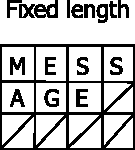
\includegraphics[height=3.4em]{chap2/fig5a}
		\caption{}
	\end{subfigure}	
	\begin{subfigure}[b]{0.3\textwidth}
		\centering
		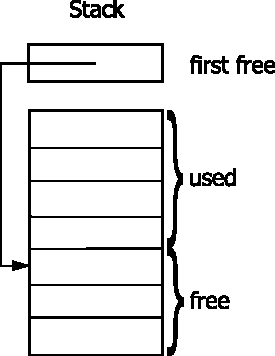
\includegraphics[height=8.1em]{chap2/fig5b}
		\caption{}
	\end{subfigure}	
	\begin{subfigure}[b]{0.45\textwidth}
		\centering
		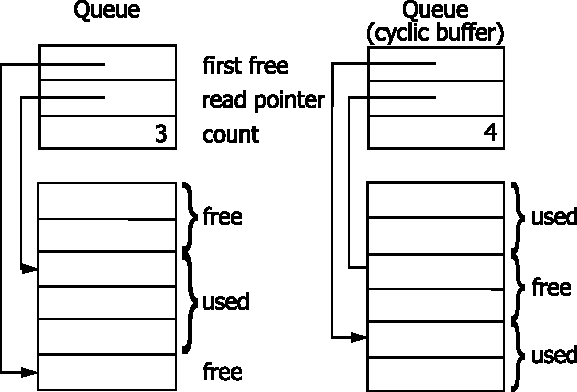
\includegraphics[height=9em]{chap2/fig5c}
		\caption{}
	\end{subfigure}	
	\caption{序列（连续表示）}
\end{figure}

序列各项长度可变时，通常不必把较短项填充到最大长度，因为可以用判别标记字段或其他技术指出任一项的长度；读入该项时，便可以据此让指针移动正确的距离。但这要求在写入时就知道读取方向，如栈或队列的情况。如果要从两端读取，就必须保证，既能从项的开头推断其长度，也能从末尾推断；这需要在序列各项之间存储冗余信息（例如前一项的长度）。

\begin{figure}[h]
	\centering
	\begin{subfigure}[b]{0.3\textwidth}
		\centering
		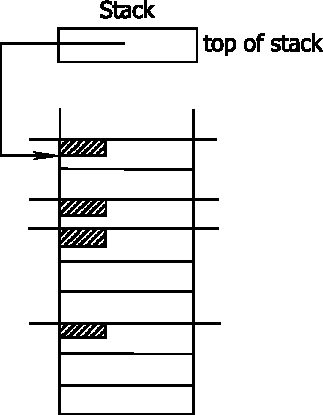
\includegraphics[height=8.4em]{chap2/fig6a}
		\caption{}
	\end{subfigure}	
	\begin{subfigure}[b]{0.3\textwidth}
		\centering
		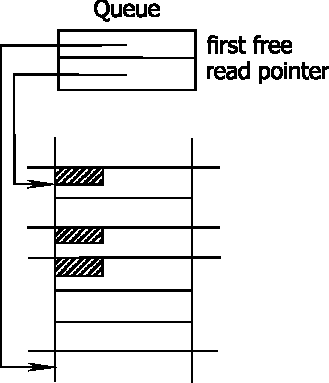
\includegraphics[height=8em]{chap2/fig6b}
		\caption{}
	\end{subfigure}	
	\begin{subfigure}[b]{0.3\textwidth}
		\centering
		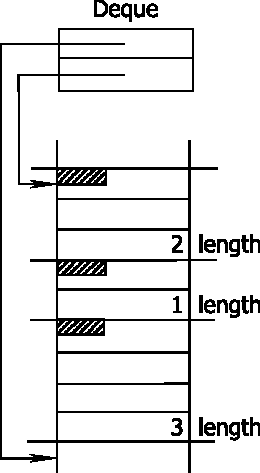
\includegraphics[height=10em]{chap2/fig6c}
		\caption{}
	\end{subfigure}
	
	\begin{subfigure}[t]{0.15\textwidth}
		\centering
		
\includegraphics[height=.4em]{chap2/fig6tag}
	\end{subfigure}
	\caption{序列（变长项）}
\end{figure}

一个序列本身是另一个序列某一项的一部分时，可以对这个项内序列采用连续表示。通常还要附一个计数，给出序列长度，以便读取项时计算其实际大小。

\subsubsection{链式表示}

为避免上一小节提到的重新移动安排问题，通常引入间接或链式存储分配方法，分配单位可以是固定长度，也可以是可变长度。可用存储空间被划分为若干区域，其中一些正用来保存某些序列的项，另一些空闲。空闲区域也链接成一个链式序列。每当程序员的序列需要扩展，就从空闲链中取得一个区域（或区域的一部分）；每当读取使序列缩短，就可以把一个区域归还空闲链。对于定长项，采用显式释放来管理动态存储分配并不困难。这里不讨论变长分配的问题；最好用分块来避免它们（见下一小节）。

最简单的链是单链。序列的每一项都附带一个链接单元，存放链中下一项的地址。空序列用一个不可能是地址的值表示（例如零或负一）；序列最后一项的链接单元也存放这个值。序列的基址单元指向链的第一项。

已知序列读取方向时，单链很有用，因为链接必须指向这个方向。对于栈，链接向后指；对于输入序列、输出序列和队列，则向前指。对于输入或输出序列，用于保存序列初值和$/$或终值的外部变量，其基址单元始终指向链的开头，而序列自身的基址单元则逐步沿序列前进。对于队列，使用两个基址单元，分别指向序列的两端。

\begin{figure}[h]
	\centering
	\begin{subfigure}[b]{0.3\textwidth}
		\centering
		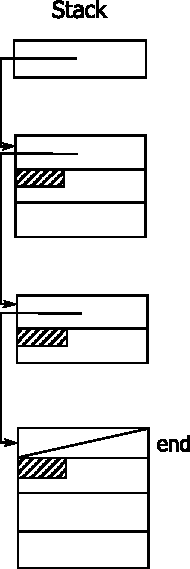
\includegraphics[height=12em]{chap2/fig7a}
		\caption{}
	\end{subfigure}
	\begin{subfigure}[b]{0.3\textwidth}
		\centering
		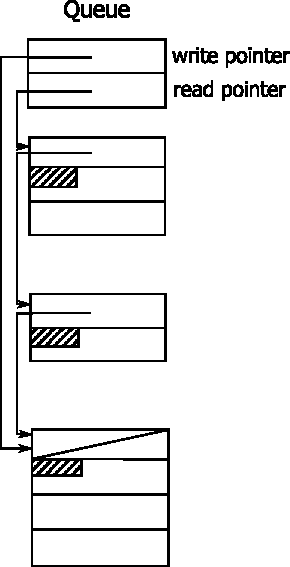
\includegraphics[height=12em]{chap2/fig7b}
		\caption{}
	\end{subfigure}
	\begin{subfigure}[b]{0.3\textwidth}
		\centering
		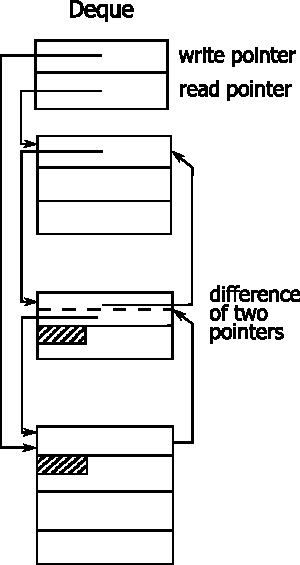
\includegraphics[height=12em]{chap2/fig7c}
		\caption{}
	\end{subfigure}
	\caption{序列（链式表示）}
\end{figure}

对于栈，单链表示的一个可能优点，是多个栈可以共享相同的起始部分，从而在某些应用中节省空间和时间。不过，从这种栈中弹出一项时，不能立即把它占用的存储空间归还空闲链，因为它可能仍被其他栈使用。一种解决办法是从不显式归还空间，而是等空闲链耗尽。然后扫描所有当前已分配的序列，标记所有正在使用的块，再把所有未标记的块收集到空闲链。这称为扫描—标记—收集式垃圾回收。它看起来免除了程序员显式控制主存分配和释放的责任，但在复杂的计算机应用中，这种责任不能轻易回避，因此这样做可能有危险。

对于需要双向读取的双端队列，单链已经不够。通常的解决办法，是为链中的每一项附加\textit{两个}指针，一个指向前一项，另一个指向后一项。实际上，这两个指针可以压缩到一个字中，只存它们的差。由于第一项和最后一项中的一个指针为标准空值，总可以通过减法得到这些项中另一个指针的值。读写时，可以方便地调整新的第一项或最后一项的链接单元值，因为此时仍知道原来第一项或最后一项的地址。这一方案的具体推导留作练习。

链接各项的另一种方法，是把所有链接汇集到一个连续的表中，最好是定长表。这就给出了序列的一种树形表示，便于双向扫描。但它给序列的项数设定了上限，而且意味着链接所用的存储单元必须永久分配，即使序列很短也是如此。可以用分块减轻这一问题。

\subsubsection{分块表示}

链式表示的一个缺点，是需要额外空间保存链接，而且每次操作都要花时间管理空闲存储链。序列各项很小而序列很长时，这些问题尤其严重。解决方法是分块，即把连续存储和链式技术结合起来。

这种技术分配一个定长存储块，足以容纳大约十到一百个项。块填满后，用上一小节介绍的任意方法把新块链接到它后面。输入时，只有一个块中的所有项都被扫描完，才把该块归还空闲存储区。这样，链接占用的存储量可以降到微不足道的程度。对链的树形表示，这尤其有利。

如前所述，分块还能避免变长动态存储分配带来的问题，因为可以让所有序列都采用相同的固定块大小，不受各项大小的影响。此外，如果序列的一部分或全部保存在辅助存储器上，几乎都应当采用分块，因为传送单位太小时，辅助存储传送可能十分低效。分块唯一的（也值得怀疑的）缺点，是妨碍有效共享栈的尾部。

剩下的唯一问题，是选择适合各种用途的块大小。显然，它必须足够大，能容纳任一序列中的最大项。实际上，它还应大到至少容纳十个典型项；否则，块末尾不足以容纳下一项的剩余空间，可能占相当大的比例。此外，如果序列部分或全部保存在辅助存储器上，块应足够长，保证不会在块间间隙中浪费过多空间；传送频率也应足够低，保证不会把过多时间耗在启停、等待或磁头移动延迟上。

另一方面，如果块太大，第一个块开头和$/$或最后一个块末尾浪费的空间就会变得显著。因此，块也应足够小，保证典型序列至少占十个块。

面对这么多相互冲突的考虑，很难为长度和项大小各不相同的序列，以及采用不同访问方法的各种辅助存储器，选择统一的块大小。不过，往往可以作出一个可接受的折中；在当今计算机设计中，128 到 1024 个字的块通常是合适选择。大多数情况下，选定的大小即使增至两倍或减半，可能也不会有决定性影响。

\subsubsection{辅助存储表示}

处理序列时，程序通常只需访问它的一端，而中间和另一端的内容会在相当长的时间内不被使用。如果主存略有不足，把这些内容转移到辅助存储器就很有利，它们占用的主存空间可以用于其他用途。对于生存期长于读写它们的程序的输入和输出序列，几乎必须用辅助存储器长期保存。

采用辅助存储器时，处理和表示的效率要求按大小合理的块传送。包含序列活动端的块始终保留在主存中；为了让输入$/$输出与计算重叠进行，写入时的前一个块，或读取时的下一个块，在传送期间也保留已分配的空间。这称为双缓冲。还可以在存储器中保留更多缓冲区，平滑处理速度与传送速度的波动；但程序设计者不能误以为，这能解决处理速度与传送速度根本不匹配的问题。一般而言，如果双缓冲或三缓冲不够，再用更多缓冲区填满存储器，也不值得。

机器具有自动分页机制时，序列表示的问题会大大减轻。对程序员而言，只需采用连续表示，为最长可能序列分配所需空间。这实际上不应浪费存储，因为分页系统应推迟实际分配，直到空间第一次使用。随着序列扩展，会分配新的存储块，但在程序员看来，这些块的地址是连续的；因此，不会有块末空间不足以容纳下一项而闲置的问题。一个块填满后不久，就会自动迁移到辅助存储器；一旦需要，又会自动调回。对于输入序列，扫描完一个块以后不久，它也会从主存移走；但如果自上次读入以来内容未变，就不会产生不必要的辅助存储传送。分页系统唯一不会自动进行的操作，是在实际需要之前，预先把输入序列的一个块读入主存。
\section[递归数据结构]{递归数据结构}

数据结构化的方法，与处理这些数据的程序的结构化方法之间，存在一些密切的类比。因此，笛卡尔积对应复合语句，后者给各分量赋值。类似地，带判别标记的联合对应条件构造或 case 构造，为每种备选情况选择合适的处理方法。数组和幂集对应依次遍历其元素的 for 语句，迭代次数本质上有界。

序列结构是第一个允许构造基数无限、值的长度无界的类型的结构；它对应无界循环，用 \textbf{while} 条件控制终止。序列之所以无界，是因为构成它的一个分量（即前段）属于与自身相同的类型；正如 \textbf{while} 循环执行一次迭代以后，剩下要执行的语句与迭代前是同一条语句。

自然会问：这种类比能否推广到与递归过程相对应的数据结构？这种类型的一个值，可以包含不止一个与自身同类型的分量；正如递归过程可以在过程体中的多个位置递归调用自身。与递归过程一样，可以直接把正在定义的类型名写进其自身定义，方便地定义这种结构；对于相互递归的定义，也可以把类型名写在先前某个类型的定义中。

递归数据结构最明显的例子，来自对程序设计语言中算术表达式或逻辑表达式的描述；这里的递归反映了一个表达式可以嵌套在另一个表达式中的可能性。例如，算术表达式可以定义如下：

“表达式是一系列项，每一项由一个符号 $(+ \text{ 或 } -)$ 后接一个因子序列组成。除第一个因子外，每个因子都由一个符号 $(\times \text{ 或 } /)$ 后接一个基本表达式（primary）组成。基本表达式要么是常量，要么是变量，要么是括号括起来的表达式。表达式开头的正号可以省略。”

只需使用已经熟悉的技术，再加上递归，就能定义一个以这类表达式为值的结构化数据类型：

\quad \textbf{type} expression $=$ \textbf{sequence} term;

\quad \textbf{type} term $= ($addop:operator; $f$:\textbf{sequence} factor$)$;

\quad \textbf{type} factor $= ($mulop:operator; $p$:primary$)$;

\quad \textbf{type} primary $= ($const:$($val:real$)$,

\tabto*{9.3em}var:$(id$:identifier$)$,

\tabto*{9.3em}bracketed:$(e$:expression$))$;

\quad \textbf{type} operator $= ($plus, minus, times, div$)$;

这个定义表达算术表达式的抽象结构，却不涉及其作为字符串的具体表示细节。例如，它没有规定括号和运算符使用什么符号，也没有说明采用中缀、前缀还是后缀记法；没有说明如何区分三种基本表达式；甚至没有表示表达式第一项的 plus 可以省略，以及每项第一个因子的 $\times$ 必须省略。除去这种抽象程度和表示无关性，这个类型定义对应于一组 BNF 语法方程：

\quad $\langle$expression$\rangle ::= \langle$term$\rangle\ |\ \langle$addop$\rangle \langle$term$\rangle\ |\ \langle$expression$\rangle \langle$addop$\rangle \langle$term$\rangle$

\quad $\langle$term$\rangle ::= \langle$primary$\rangle\ |\ \langle$term$\rangle\langle$mulop$\rangle\langle$primary$\rangle$

\quad $\langle$primary$\rangle ::= \langle$unsigned real number$\rangle\ |\ \langle$variable$\rangle\ |\ (\langle$expression$\rangle)$

注意，我们尽可能用序列替代了递归。实际上，只要类型名在其定义的开头或末尾递归出现一次，就能这样做。例如：

\quad \textbf{type} expression $=$ \textbf{sequence} term;

\noindent
本可以递归地写成：

\quad \textbf{type} expression $= ($empty:$()$, non-empty:$($first:term; final:expression$))$.

\noindent
类似的替代表述，也能把 \textbf{while} 循环表达为递归过程。

构造递归定义类型的值，不需要新的运算符或转换函数；只需递归地使用为其他相关结构化方法定义的那些方法。例如，表达式

\quad $3/(b - 2)$

\noindent
可以用以下繁琐的构造指定：

\quad $[$term $($plus, $[$factor (times, primary $($const$(3)))$,

\tabto*{7.75em} factor $($div, primary $($bracketed $($

\tabto*{9em}  $[$term $($plus, $[$factor $($times, primary $($var$($``$b$''$)))]),$

\tabto*{9.1em}  term $($minus, $[$factor $($times, primary $($const$(2)))])])))$

\tabto*{7.55em}  $])$

\quad $]$.

\noindent
后面将在（\ref{sec:example-9-2}）中举例，介绍让计算机自己把表达式翻译为抽象结构的有效方法。

递归定义的数据的另一个熟悉例子，是家谱。家谱（不包括婚姻信息）可以这样定义：为每个人关联其所有子女各自的家谱。假定还需要保存一些个人详细信息：

\quad \textbf{type} family $= ($head:person; offspring:\textbf{sequence} family$)$;

没有子女的人，是家谱的最终分量，可以表示为：

\quad family$($Tom, $[])$

\noindent
有三个孩子的家庭可以表示为：

\noindent
family $($Jill, $[$family $($Tom, $[])$,

\tabto{3.2em} family $($Joanna, $[])$,

\tabto{3.2em} family $($Matthew, $[])])$.

最后一个例子说明，如何把 LISP 程序员熟悉的二叉树定义为递归数据结构。

\quad \textbf{type} list $= ($atom:\textbf{sequence} character, cons:$($car, cdr:list$))$.

\noindent
一个表在 LISP 的点记法中写成：

\quad $(($A.$($B.NIL$))$.NIL$)$

\noindent
它可以用几乎与 LISP 完全相同的方式，表达为 list 类型的值：

\quad cons $($cons $($atom $($``A''$)$,

\tabto{5em} cons $($atom $($``B''$)$, atom $($``NIL''$)))$,

\tabto{5em} atom $($``NIL''$)$

\tabto{4.8em} $)$;

\noindent
其中，转换为 list 类型的操作省略不写。

作为处理表的例子，我们编写一个函数，把整棵树翻转，使每个“左分支”变为“右分支”，反之亦然。

\quad \textbf{function} reverse$(l$:list$)$:list;

\quad \quad \textbf{with} $l$ \textbf{do}

\quad \quad \quad $\{$atom:reverse $\coloneq l$,

\quad \quad \quad ~ cons: reverse $\coloneq$ cons$($reverse$($cdr$)$, reverse $($car$))\}$

\subsection{表示}

递归类型的标准表示，与结构类似的非递归类型也很相近，区别在于：声明为递归类型自身的每个分量，不直接保存其值，而是用一个保存指向该值的指针的存储单元来表示。采用指针，是因为分量值的大小可能任意，无法分配固定数量的存储空间来容纳它。这称为“树形表示”，类似于数组或序列的树形表示，只是各分支可以增长到任意且不同的高度。

另一种表示方法是线性序列或\textit{位流}（bitstream）。这种表示可以不用指针，把递归子结构的值与其余信息连续存放，就像熟悉的、带括号的表达式字符表示一样。不过，我们可以根据上下文恢复括号结构，必要时扫描联合值的判别标记，而不用实际括号。这种方法通常与其他分量的紧缩表示结合使用，可以显著减少存储空间，代价是必须顺序访问结构中的各个分量。在许多情况下，位流表示的大小大约只有树形表示的十分之一。

\begin{figure}[h]
	\begin{subfigure}[t]{\textwidth}
		\centering
		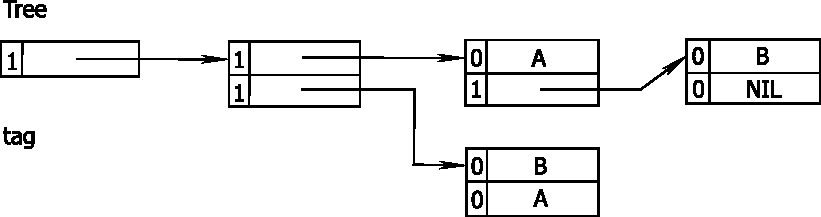
\includegraphics[width=.7\textwidth]{chap2/fig8a}
		\caption{}
	\end{subfigure}
	
	\begin{subfigure}[t]{\textwidth}
		\centering
		
\includegraphics[width=.58\textwidth]{chap2/fig8b}
		\caption{}
	\end{subfigure}
	\caption{(($A$\,.\,($B$.NIL))\,.\,($B$\,.\,$A$) 的表示}
\end{figure}

树形表示与线性表示之间的选择通常很明显。如果程序正在处理结构，通常是通过递归过程处理，那么方便访问任一分量的需要，就决定了应采用树形表示。此外，可以让多棵树共享公共分支，收回部分空间开销；共享分支是符号表达式处理的一个特点。但如果结构需要输出，随后重新输入，线性结构就优越得多。它不仅通过减少数据量缩短传送时间，线性化还避免了在辅助存储器上表示指针的许多棘手问题。许多情况下，一个结构经历多个处理和输入输出阶段，会在每个阶段转换表示；高级程序设计语言的多遍翻译程序就普遍这样做。

必须注意，共享递归子结构只是一种节省时间和存储空间的手段，对程序运行没有影响。这意味着，只要共享子结构有可能作为某个所属结构的一部分而被选择性更新，就必须避免共享。原则上，所有值彼此完全分离，程序员既无法知道，也无须关心自己的结构有多少部分被共享。此外，绝不可能让一个指针指回它所属的结构，因为这意味着该结构与自身的一个分量相同。只有无限结构才可能具有这种性质；而无限结构不满足排除公理，递归结构的重要归纳原理正是以这一公理为基础的。

\subsection{例子}
\label{sec:example-9-2}

程序设计语言中表达式的源文本，以如下定义的符号序列给出：

\quad \textbf{type} symbol $= ($constant:$($value:real$)$, variable:$($identifier: ident$)$,

\tabto*{9.2em}op:operator, leftbracket, rightbracket$)$;

编写一个程序，操作输入变量

\quad source:\textbf{sequence} symbol,

\noindent
从其开头读取尽可能长的合法表达式，返回相应的抽象表达式；如果无法做到，就转到标号 error 退出。结果的结构和源文本的语法，如本节前面所述。

程序结构紧密遵循所需结果的结构。有三个函数：

\quad compile expression

\quad compile term $($sign$)$

\quad compile primary

\noindent
每个函数都从 source 中移除其语法类别下最长的表达式，并返回相应的抽象结构。主要的特殊之处是，表达式的第一项可以没有符号；因此，sign 作为参数传给 compile term，而不是由 compile term 自己从 source 中读取。每个函数成功时，都有缩短 source 序列的副作用；失败时，则跳转到 error。

\noindent
\textbf{function} compile expression:expression;

\noindent
\quad \textbf{begin} sign:operator;

\noindent
\quad \quad \textbf{if} source.first $=$ plus $\vee$ source.first $=$ minus \textbf{then} sign \textbf{from} source

\noindent
\quad \quad \textbf{else} sign $\coloneq$ plus;

\noindent
\quad \quad compile expression $\coloneq [$compile term$($sign$)]$;

\noindent
\quad \quad \textbf{while} source.first $=$ plus $\vee$ source.first $=$ minus \textbf{do}

\noindent
\quad \quad \quad \textbf{begin} sign \textbf{from} source;

\noindent
\quad \quad \quad \quad compile expression$\wideparen{\text{:\ }[}$compile term$($sign$)]$

\noindent
\quad \quad \quad \textbf{end}

\noindent
\quad \textbf{end};

\noindent
\textbf{function} compile term$(s$:operator$)$:term;

\noindent
\quad \textbf{begin} $p$:primary; sign:operator; $fs$:\textbf{sequence} factor;

\noindent
\quad \quad $p\coloneq$ compile primary;

\noindent
\quad \quad $fs \coloneq [$factor(times, $p)]$;

\noindent
\quad \quad \textbf{while} source.first $=$ times $\vee$ source.first $=$ div \textbf{do}

\noindent
\quad \quad \quad \textbf{begin} sign \textbf{from} source:

\noindent
\quad \quad \quad \quad $p\coloneq$ compile primary;

\noindent
\quad \quad \quad \quad $fs\wideparen{\text{: }[}$factor$($sign, $p)]$

\noindent
\quad \quad \quad \textbf{end};

\noindent
\quad \quad compile term $\coloneq$ term$(s$, $fs)$

\noindent
\textbf{function} compile primary:primary;

\noindent
\quad \textbf{begin} $s$:symbol;

\noindent
\quad \quad $s$ \textbf{from} source;

\noindent
\quad \quad \textbf{with} $s$ \textbf{do} $\{$constant:compile primary $\coloneq$ const$($value$)$,

\noindent
\quad \quad \quad variable:compile primary $\coloneq$ var$($identifier$)$,

\noindent
\quad \quad \quad leftbracket:

\noindent
\quad \quad \quad \textbf{begin from} source;

\noindent
\quad \quad \quad \quad compile primary $\coloneq$ bracketed$($compile expression$)$;

\noindent
\quad \quad \quad \quad $s$ \textbf{from} source;

\noindent
\quad \quad \quad \quad \textbf{if} $s \neq$ rightbracket \textbf{then go to} error

\noindent
\quad \quad \quad \textbf{end},

\noindent
\quad \quad \textbf{else go to} error$\}$

\noindent
\quad \textbf{end};

\noindent
\textit{练习}
\nopagebreak

\noindent
编写程序，把表达式从树形表示转换为位流，再转换回来。
\section[稀疏数据结构]{稀疏数据结构}
\label{sec:sparse-data-structures}

讨论数组和幂集的表示时，迄今一直假定幂集的基类型和数组的定义域类型比较小，可以为结构中每个潜在元素分配一个位，或更大的存储区域来保存其值。例子也限于这类情况。本节研究基类型或定义域类型很大乃至无限、因而标准表示不再可行时，会带来什么后果和问题。

幂集及无限定义域映射，仍可以表示和操纵，条件是只考虑含有限个元素的集合，以及只有有限个元素取有意义值的映射；这里，“有意义”定义为不同于某个指定的空值或默认值。无限集合的幂集显然也是无限的；但由于这里幂集类型的每个值都只含有限个元素，只需在有限时间内列出这些元素，就能指定每个值，而列表也只占有限存储空间。类似地，对于定义域无限的映射类型，可以列出定义域中所有映射到有意义值的元素，并同时列出各自映射到的值域值，从而有限地指定其每个值。受到这种限制的类型，称为\textit{稀疏}类型。

实际上，稀疏性并不限于无限的基类型和定义域；它也适用于很大但有限的幂集，前提是程序员知道，自己关心的每个实际集合只会包含潜在元素中极小的一部分。例如，基类型可能包含数亿个值，但程序员知道只需处理大小不足一百的集合，而其中大多数甚至不足十。位模式表示会需要数亿个位，不可能采用；但由于程序中实际使用的每个值只有少数元素，用相对很少的空间就能方便地列出它们。这种幂集类型称为\textit{稀疏}幂集类型。类似地，定义域很大、其中几乎所有元素都映射到同一个默认值域值的数组，被称为属于\textit{稀疏数组}类型。

高级数据处理应用经常遇到稀疏集合和数组，其表示和操纵会带来一些熟悉的问题。第一个例子，是定义以车牌号码集合为值的类型。carnumber 类型的基数可能大约是四十亿；但程序员只想处理单个人所拥有汽车的集合，其中大多数只有一个元素，超过十个的极少。因此，carset 类型可以声明为稀疏幂集：

\quad \textbf{type} carset $=$ \textbf{sparse powerset} carnumber;

作为稀疏数组的例子，可以考虑从车主到其所拥有汽车集合的映射类型。每位车主以姓名和地址表示；两者长度任意，所以 owner 类型可以定义为：

\quad \textbf{type} owner $=$ \textbf{sequence} character;

\noindent
它的基数无限。因此，所需类型声明为稀疏类型：

\quad \textbf{type} carfile $=$ \textbf{sparse array} owner \textbf{of} carset.

在数据处理应用中，carfile 类型的变量称为\textit{随机访问}文件，而 owner 称为文件的\textit{键}元素。

接下来的两个例子来自数值应用。向量是从整数到浮点数的映射。稀疏向量的多数元素为零；因此，它的初值是常值零函数，所有元素都保持为零，除非显式赋予其他值：

\quad \textbf{type} sparsevector $=$ \textbf{sparse array} integer \textbf{of} real.

\noindent
稀疏复数矩阵可以用类似方式定义：

\quad \textbf{type} irregular matrix $=$ \textbf{sparse array} $($row, column:integer$)$ \textbf{of} complex.

下一个例子来自把程序设计语言翻译成机器码的工作。翻译过程中，翻译程序需要知道源程序中每个已声明标识符的某些信息，例如为变量分配的机器地址、长度、类型等等。假定这些信息属于 decode 类型。为每个标识符关联一个 decode 值的数组类型，命名为 dictionary，声明如下：

\quad \textbf{type} dictionary $=$ \textbf{sparse array} ident \textbf{of} decode

\noindent
当然，翻译程序只关心源程序中实际声明的那些标识符的 decode。对于绝大多数可能的标识符，这个类型的任何 dictionary 都会给出 decode 类型中表示“标识符未声明”的那个值。

最后一个例子，是商业文件系统和现实生活中都会引发熟悉问题的一种类型\textemdash{}多维交叉分类。一家公司的客户按地域分为若干区域，也按所购产品类别分为若干类别。有时需要访问某一区域的所有客户，依次遍历各类别；有时需要访问某一类别的所有客户，依次遍历各区域；最后，有时需要处理某一区域中某一类别的所有客户。处理这种情况所需的抽象结构，是一个以稀疏集合为元素的二维稀疏数组：

\quad \textbf{sparse array} $(c$:class; $a$:area$)$ \textbf{of sparse powerset} customer.

描述人与人的家庭关系时，也可能出现类似例子：

\quad \textbf{type} children $=$ \textbf{sparse array} $($mother, father:person$)$ \textbf{of} 

\tabto*{9.2em}\textbf{sparse powerset} person;

\noindent
对于涉及多次婚姻的情况，这个数组比可以定义为递归结构的、更接近树形的家庭表示更合适。

对于稀疏数组，有时把它们看作偏映射，而不是全映射，会很有用。偏映射不一定为定义域类型的每个元素都给出一个值。换言之，它实际有定义的定义域，是定义域类型的一个子集。对于这种数组类型，需要引入附加常量 omega，表示处处未定义的映射。再引入函数

\quad domain$(x)$

\noindent
也很有用，它返回一个集合，包含 $x$ 中实际有定义的元素的下标。因此，程序员可以遍历所有已定义的元素，或测试某个具体元素是否有定义。上述许多例子也完全可以声明为偏映射，而不是稀疏映射。对于偏映射，不必记录默认值。

\subsection{表示}

\noindent
稀疏集合和数组的通常表示，只记录默认值和那些有意义的元素。因此，这种表示借用序列类型处理大小可变结构的技术。稀疏集合可以看作稀疏映射的特例：把所有集合元素映射为布尔值 true，把所有非集合元素映射为默认值 false。因此，它们的表示与稀疏数组非常相似，不必单独讨论。

稀疏映射由若干元素组成。映射的每个元素都表示为其下标与值的笛卡尔积；这里，下标称为\textit{键}，值称为与该元素关联的\textit{信息}，两者并置在一起就称为一个\textit{条目}。对于稀疏集合，不需要记录任何信息，因为键本身的存在，足以表明该值是集合的元素。因此，稀疏集合的条目只包含键。

\subsubsection{顺序表示}

稀疏数组类型最简单的表示，是条目的序列；
即：

\quad \textbf{sparse array} $D$ \textbf{of} $R$

\noindent
表示得仿佛原先声明为：

\quad $($default:$R$; $s$:\textbf{sequence} $($key:$D$; information:$R))$.

现在，必须按选择序列表示时的同样准则，从各种可能的序列表示中选出一种。但用序列表示稀疏数组时，条目顺序无关紧要，无须反映它们加入的先后时间。因此，常常把条目按其
键值排序，尤其是当以后也将按这个顺序扫描时。

顺序表示的主要缺点，是访问任意给定下标对应的元素所需时间很长。对于规模较大的结构，程序设计者通常会花相当大的力气，确保按条目在序列中存储的同一标准顺序访问它们；如果要插入新条目，也先排序，再与原序列归并。因此，商业应用中标准的批处理和顺序文件更新方法，可以视为在不太适合随机访问的磁带介质上，实现稀疏数组这一抽象概念的实用办法。

\subsubsection{表式表示}

如果稀疏映射的条目个数有一个足够小、可以接受的上限 $N$，表式表示就能显著提高查找速度。其中，稀疏映射

\quad \textbf{sparse array} $D$ \textbf{of} $R$

\noindent
表示为非稀疏数组：

\quad $($default:$R$; occupied:\textbf{powerset} $0\,.\,.\,N$;

\tabto*{8em}\textbf{array} $0\,.\,.\,N$ \textbf{of} $($key:$D$; information:$R))$.

\noindent
如果所有有意义的条目都在使用之前收集完毕，就可以把表排序，然后用对数时间的查找，快速找到给定键对应的条目。

如果访问数组元素与添加新条目交替进行，就适合采用某种散列表技术。为此，选定一个任意的“散列”函数，把定义域类型 $D$ 映射为 $0\,.\,.\,N$ 范围内的整数。插入条目时，把它放在表中这个位置；以后访问它时，使用同一散列函数就能在这里找到它。如果该位置已经被另一个键不同的条目占用，就必须在表中寻找其他空位置。通常会搜索表中紧接着的后续位置；但表快满时，这可能使条目在某个恰好热门的区域周围不理想地聚集。解决办法之一，是选择 $N + 1$ 为素数，并用第二个散列函数从给定键算出任意步长。如果某位置已满，就把这个步长加到前一个位置上（模 $N + 1$），得到下一个要尝试的位置。

\subsubsection{索引表示}

表式存储方法只适合整张表都能
容纳在计算机主存中的情况。通常，如果
无法做到这一点，就把表式与顺序方法
结合使用。此时，把稀疏数组表示为一个表，其中每个
条目都是序列：

\quad $($default:$R$; table:\textbf{array} $1\,.\,.\,N$ \textbf{of}

\tabto*{10em}$($max:$D$; seq:\textbf{sequence} $($key:$D$; information:$R)))$.

\noindent
每个条目都放在这样一个序列 $i$ 中：其键落在 table $[i - 1]$.max（$i = 1$ 时为 $D$.min）与 table $[i]$.max 之间。表按序排列，以便快速定位合适的序列。这种技术类似多卷百科全书的编排：每卷书脊上注明该卷第一个和最后一个条目的键，不必把书从书架上取下，就能迅速识别正确的卷。

采用这种表示时，最好保证各序列长度大致相同。特别是，如果使用磁盘辅助存储器，让每个序列都放在单个柱面内非常有利，因为一次随机访问就不会需要多于一次磁头移动。因此，当某个序列过长时，它必须与相邻序列交换内容。这需要提取键最大和/或最小的条目；所有序列都已按键值排序时，最容易完成。排序和重新安排常常作为独立操作，定期进行；这种文件组织的总体方法称为“索引顺序”组织。

自然，在这种表示方法中，序列应尽可能短，例如短于磁盘上的一个磁道。因此，表本身可能变得很大，主存不再能容纳。这时，把表本身也分成若干段，再次使用同一原则，建立一个指向各段的第二级表。因此，每次访问数组元素，通常至少需要两次辅助存储访问。强烈建议，选择序列和表段的大小与位置时，应使它们与存储介质的访问特性紧密对应。

\subsubsection{局部稠密表示}

数值计算应用中遇到的一种特殊稀疏数组，是稀疏矩阵。稀疏矩阵常常可以划分为多个子矩阵，其中只有少数包含有意义的非零条目。这种情况下，可以说矩阵是局部稠密的，表示和处理时应利用这一事实。

一种方法，是为每个有意义的子矩阵保存其位置和大小，并把整个矩阵表示为这些子矩阵的表或序列；每个子矩阵按通常方式连续存储，使用乘法计算地址。不过，各子矩阵大小一般不同；如果处理矩阵时大小还会变化，问题就很严重。一种可能的方法，是把稀疏矩阵分成标准大小的子矩阵，例如十六乘十六，并建立一个表，保存指向各子矩阵的指针。全零子矩阵用空指针表示，不占其他存储空间；否则，按通常方式存储子矩阵，采用下面的地址计算方法。

每次访问数组时，先把两个下标的位值“交错”排列，使结果的最低有效部分包含两个下标各自的最低有效部分。随后，用结果的较高有效部分查地址表，定位所需子矩阵；用较低有效部分找到所需元素在子矩阵中的位置。某些机器上，这种下标交错技术可能比一般乘法更高效。如果某些子矩阵必须保存在辅助存储器中，就特别推荐这种地址计算方法，因为它按行处理矩阵与按列处理同样高效。因此，对于所有大型数组，无论是否稀疏，都可以推荐这种方法，尤其是在采用分页的计算机上。该方法的发明者是 E. W. Dijkstra 教授。

\subsubsection{网格表示}

文件交叉分类，在计算机上引起的问题与现实生活中一样多。通常的解决办法，是把最方便的一种分类作为标准，接受按另一种分类处理的额外成本，即使这需要重新排序文件。因此，稀疏映射

\quad \textbf{sparse array} $(i:D_1; j:D_2)$ \textbf{of} $R$

\noindent
表示为：

\quad \textbf{sparse array} $D_1$ \textbf{of} $($\textbf{sparse array} $D_2$ \textbf{of} $R)$

不过，也可以采用基于序列链式表示的方法，更对称地处理两个维度。在这种表示中，把 $D_1$ 的每个实际使用值放入一条链，把 $D_2$ 的每个实际使用值放入另一条链；这两条链称为\textit{边界链}。任一边界链的每个元素，都包含一个基址单元，指向具有该分类键值的所有元素组成的链式序列。现在，数组的每个实际条目都附有\textit{两个}地址：一个指向按 $D_1$ 分类时属于同一类的序列中的下一项，另一个指向按 $D_2$ 分类时属于同一类的下一项。因此，可以把每个项想象成位于二维网格线的一个交点，指针分别横向和纵向指向同一行或同一列的下一项。

\begin{figure}[h]
	\centering
	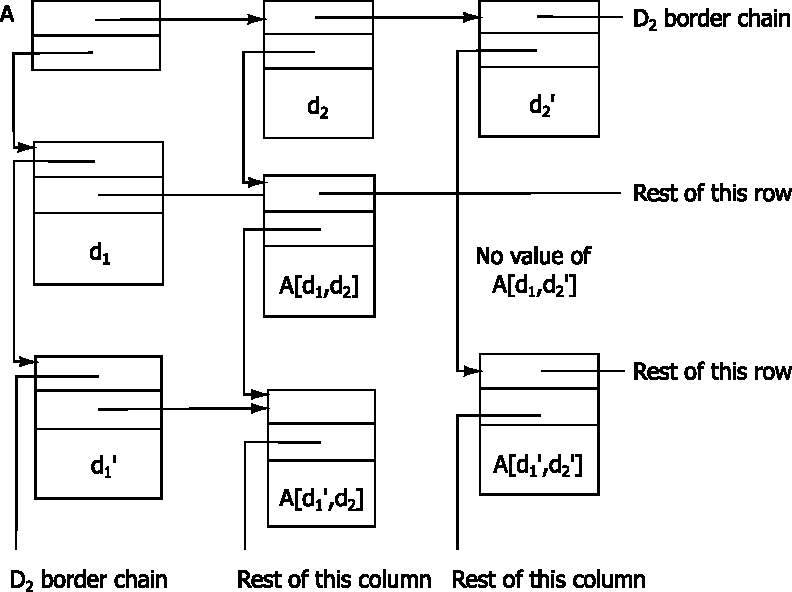
\includegraphics[width=.7\textwidth]{chap2/fig9}
	\caption{$A$: \textbf{sparse array} $(d_1: D_1;\ d_2: D_2)$ \textbf{of} $T$ 的网格表示}
\end{figure}

遗憾的是，这种网格表示只适合整个结构都能放入主存的情况。如果序列的大部分必须保存在辅助存储器中，为了效率，就应对相邻元素采用某种分块方法。
\section[例子：考试时间表]{例子：考试时间表}
\label{sec:example-examination}

在允许学生自由选择多种课程组合的教育机构中，需要编排这样一份考试时间表：每门考试只安排在一个时段，同时每位学生都能参加自己所修各门课程的考试。为每门考试单独分配一个时段，总能做到这一点；但无论考官还是学生，都希望整个考试期尽可能短。这意味着，每个时段应尽可能多地安排考试，但不能超过某个上限 $k$。考场大小还带来另一个约束：它只能容纳一定数量的学生。

在设计程序之前，最好根据各种已给定及所需数据项的结构，作更严格的形式化描述，以确认我们对问题的理解。“student”和“exam”类型显然是非结构化的，现阶段无须进一步定义。每位学生需要参加的考试，由一个映射给出：

\quad load:\textbf{array} student \textbf{of powerset} exam.

\noindent
时间表是时段的集合，而每个时段又由考试的集合组成：

\quad \textbf{type} session $=$ \textbf{powerset} exam;

\quad timetable:\textbf{powerset} session.

\noindent
接下来，尝试把输入和输出数据应具备的性质形式化。

\begin{enumerate}[wide, nosep, label=(\arabic*)]
	\item \label{en:examination-1}
	我们决定不把“时段个数最少”这一条件形式化，因为如果计算绝对最小值代价过高，我们实际上并不要求绝对最小值。

	\item \label{en:examination-2}
	每门考试都安排在某个时段：

	$\displaystyle\bigcup_{s\text{ \textbf{in} timetable}} s =$ exam.all
	\smallskip

	\item \label{en:examination-3}
	任何考试都不安排在多个时段：

	\quad $(s1 \wedge s2 = \{\})$ 或 $(s1 = s2)$

	\noindent
	条件 \ref{en:examination-2} 和 \ref{en:examination-3} 实际上说明，时间表把全部考试的集合划分为一组覆盖全部且互不相交的子集。

	\item \label{en:examination-4}
	任何时段都不包含超过 $k$ 门考试：

	\quad $s$ \textbf{in} timetable $\supset$ size$(s) \leqslant k$

	\item \label{en:examination-5}
	任何时段涉及的学生人数都不超过 hallsize。要形式化这一点，需要统计参加每门考试的学生人数：
	
	\quad examcount$(e$:$\text{exam}) = $ size $\{st$:student $\mid$ $e$ \textbf{in} load$(st)\}$.
	
	于是，一个时段涉及的学生人数是：
	
	\quad session count$(s\text{:session}) = \displaystyle\sum_{e \text{ \textbf{in} } s}$ examcount$(e)$
	
	条件可以形式化为：
	
	\quad $s$ \textbf{in} timetable $\supset$ sessioncount$(s) \leqslant$ hallsize.
	
	\item \label{en:examination-6}
	任何学生都不会在一个时段参加多门考试。要形式化这一点，引入考试不相容的概念：如果某个学生同时需要参加两门考试，这两门考试就不相容。对于每门考试 e1，都有一个与它不相容的考试集合 incompat$(e1)$：
	
	\quad incompat$(e1)= \{e2\text{:exam}\ |\ e2 \neq e1\ \&\ \exists\ st$:student$(e1 \text{ \textbf{in}}$ load$(st)$
		
	\tabto*{8.2em} \& $e2$ \textbf{in} load$(st))\}$
\end{enumerate}

\noindent
现在可以规定，一个时段中每一对考试都必须相容：

\quad $s$ \textbf{in} timetable \& $e1$, $e2$ \textbf{in} $s \supset\neg e1$ \textbf{in} incompat$(e2)$.

这六个条件用 load、hallsize 和 $k$ 定义。现实中任何成功的时间表，以及时间表的任何成功的计算机表示，都必须满足它们。它们规定了考试排程程序的目标与正确性标准。

\subsection{抽象程序}

考察这些条件可以发现，构造时间表不需要完整了解每位学生的 load。只需要每门考试的 examcount，以及与它不相容的其他考试的集合：

\quad examcount:\textbf{array} exam \textbf{of} integer;

\quad incompat:\textbf{array} exam \textbf{of powerset} exam.

\noindent
这两个数组体现了对实际数据的抽象，恰好把注意力集中在当前目的所需要的特征上，让我们暂时忽略情境中的其他特征。显然，只扫描一次学生的 load 数据，就很容易构造出这两个数组：

\quad examcount $\coloneq$ all$(0)$;

\quad incompat $\coloneq$ all$(\{\})$;

\quad \textbf{for} $st$:student \textbf{do}

\quad \quad \textbf{for} $e$ \textbf{in} load$(st)$ \textbf{do}

\quad \quad \quad \textbf{begin} examcount$(e)$: $+\ 1$;

\quad \quad \quad \quad incompat$(e)$: $\vee\ (\text{load}(st) - \{e\})$

\quad \quad \quad \textbf{end};

寻求解法时，一个简化因素是这些条件很容易分成两类：\ref{en:examination-1}、\ref{en:examination-2} 和 \ref{en:examination-3} 针对整个时间表，而 \ref{en:examination-4}、\ref{en:examination-5} 和 \ref{en:examination-6} 只针对单个时段，根本不涉及整个时间表。因此，程序可以组织为一个内层部分，选出满足 \ref{en:examination-4}、\ref{en:examination-5} 和 \ref{en:examination-6} 的合适时段；再加一个外层循环，用这些合适时段构造时间表。

外层循环的目标，是在完成时满足条件 \ref{en:examination-2} 和 \ref{en:examination-3}。因此，选择其中一个作为循环终止条件，并把循环体设计为始终保持另一个条件成立（即循环不变式）；此外，还要保证开始循环之前，不变式已经成立。

显然可以选择互不相交性（条件 \ref{en:examination-3}）作为不变式，把覆盖全部作为终止条件，使每次执行循环体都向它推进。空时间表显然满足不变式。这样就得到如下结构的算法：

\quad timetable $\coloneq \{\}$;

\quad \textbf{while} timetable does not satisfy \ref{en:examination-2} \textbf{do}

\quad \textbf{begin} select a session satisfying \ref{en:examination-4}, \ref{en:examination-5}, \ref{en:examination-6};

\quad \quad add the session to the timetable

\quad \textbf{end};

\quad print timetable.

要使添加新时段后仍保持
不变式成立，该时段的考试必须从
尚未出现在时间表中的考试里选取。因此，引入一个
新变量保存这些剩余考试：

\quad remaining:\textbf{powerset} exam;

\noindent
它由如下不变关系定义：

\quad remaining $=$ exam.all $- \displaystyle\bigcup_{s \text{ \textbf{in} timetable}} s$.

\noindent
现在，整个程序的结构成为：

\quad timetable $\coloneq \{\}$;

\quad remaining $\coloneq$ exam.all;

\quad \textbf{while} remaining $\neq \{\}$ \textbf{do}

\quad \quad \textbf{begin} $s\coloneq$ suitable;

\quad \quad \quad timetable: $\vee\ \{s\}$;

\quad \quad \quad remaining: $-\ s$

\quad \quad \textbf{end};

\quad print timetable.

剩下的问题，是每个阶段如何选出合适时段。原则上，没有理由认为每一步的“最佳”选择，最终会产生“最佳”甚至“良好”的时间表。不过，一般看来，选择剩余考试的一种组合，使它尽量接近填满考场，或尽量接近上限 $k$，应该有利。这样，可能用一组相当紧凑的时段安排大多数学生和考试，尽管最后可能留下一个颇长的“尾巴”，包含少数学生参加的许多小型时段。虽然这不会使时段个数最少，但对大多数学生和考官可能已经相当满意。

如果不接受每一步表面上的最佳选择，就只能尝试更全局的优化；这要么涉及天文数字般的试探次数，要么需要一些复杂考虑，而这些考虑很可能只有在积累了较简单算法的实际经验之后才会显现。因此，现阶段除了希望取得好结果，也没有别的办法。

还需要编写函数：

\quad \textbf{function} suitable:session,

\noindent
从剩余考试集合中选出合适时段。一种可能的方法，是生成若干满足 \ref{en:examination-4}、\ref{en:examination-5} 和 \ref{en:examination-6} 的试探时段，选出找到的最佳者。最佳时段很可能是 sessioncount 最大的那个；但以后可能要调整选择标准，所以最好把选择过程定义为独立子程序，用于更新变量

\quad bestsofar:session;

\noindent
更新依据是以下变量的当前值：

\quad trial:session;

\quad \textbf{procedure} record

\quad \quad \textbf{if} sessioncount$($bestsofar$) <$ sessioncount $($trial$)$ \textbf{then}

\quad \quad \quad bestsofar $\coloneq$ trial.

\noindent
suitable 的结果就是 bestsofar 的最终值：

\quad suitable $\coloneq$ bestsofar.

还需编写一个过程，生成并记录一系列满足 \ref{en:examination-4}、\ref{en:examination-5} 和 \ref{en:examination-6} 的试探时段。考察这些条件可知，如果某个试探时段\textit{不}满足其中一个条件，更大的试探时段也不会满足它。换言之，找到一个\textit{不可行}的试探时段以后，不必再生成包含它的其他试探时段。因此，可以把生成过程组织为：生成已知可行的每个试探时段的所有超集，但排除已经尝试过的考试。为此，引入变量：

\quad untried:\textbf{powerset} exam,

\noindent
以及过程：

\quad \textbf{procedure} gensupersets,

\noindent
它从 untried 中给 trial 添加一个或多个考试，生成并记录 trial 的所有可行超集。这个过程将在“suitable”内部调用。

\quad \textbf{function} suitable:session;

\quad \quad \textbf{begin} trial, bestsofar:session; $e$:exam; untried:\textbf{powerset} exam;

\quad \quad \quad $e$ \textbf{from} remaining;

\quad \quad \quad trial $\coloneq$ bestsofar $\coloneq$ $\{e\}$;

\quad \quad \quad untried $\coloneq$ remaining $-$ trial $-$ incompat$(e)$;

\quad \quad \quad gensupersets;

\quad \quad \quad suitable $\coloneq$ bestsofar

\quad \quad \textbf{end};

\noindent
注意，trial 的初值是某门考试的单元素集合；该考试从剩余集合中选出，选择标准尚未确定。这样做的理由是，所选考试最终总要出现在时间表的某个时段中，不妨就放在当前这个时段。如果不先作这个选择，考试排程程序的主循环每轮都会让 gensupersets 不断生成相同的超集。

另一个重要优化，是从 untried 中移除所有与 trial 中考试不相容的考试，因为完全没有必要考虑把它们加入 trial。

生成给定 trial 的超集时，可以依次从 untried 中选出考试，加入 trial。如果结果仍有效，就记录它；trial 的新值此时就是一个合适时段，可以作为进一步生成超集的基础。这说明适合采用递归程序结构。当然，加入 trial 的考试还应从 untried 中移除，以免不必要的重复；同时，从 untried 中移除所有与刚加入考试不相容的考试，非常有利，因为以后不必再考虑它们。此外，每次调用结束后，trial 和 untried 的值必须保持原状；因此，对它们的任何修改，都必须借助 save 1 和 save 2 两个变量记录并恢复。

\textbf{procedure} gensupersets;

\quad \textbf{begin} $e$:exam; save 1, save 2:\textbf{powerset} exam;

\quad \quad record; save 1 $\coloneq$ untried;

\quad \quad \textbf{if} size$($trial$) < k$ \textbf{then}

\quad \quad \textbf{while} untried $\neq \{\}$ \textbf{do}

\quad \quad \quad \textbf{begin} $e$ \textbf{from} untried;

\quad \quad \quad \quad save $2\coloneq$ untried $\wedge$ incompat$(e)$;

\quad \quad \quad \quad untried:$-$ save 2;

\quad \quad \quad \quad trial:$\vee\ \{e\}$;

\quad \quad \quad \quad \textbf{if} sessioncount(trial) $<$ hallsize \textbf{then} gensupersets;

\quad \quad \quad \quad untried:$\vee$ save 2;

\quad \quad \quad \quad trial:$-\ \{e\}$

\quad \quad \quad \textbf{end};

\quad \quad \quad untried $\coloneq$ save 1

\quad \textbf{end} gensupersets.

这个程序的有效性取决于：trial 始终满足时间表中时段所需的条件 \ref{en:examination-4}、\ref{en:examination-5} 和 \ref{en:examination-6}，并且始终是 remaining 的子集。

理由如下：

对于 \ref{en:examination-4}：gensupersets 只有在 trial 的大小严格小于 $k$ 时，才生成超集。

对于 \ref{en:examination-5}：当 trial 的 sessioncount 大于考场容量时，绝不会进入 gensupersets（假定任何 examcount 都不大于 hallsize）。

对于 \ref{en:examination-6}：从 untried 中移除不相容集合，保证任何时刻 untried 中剩下的所有考试，都与 trial 中的所有考试相容。因此，把 untried 中任意一门考试转移到 trial，绝不会违反 \ref{en:examination-6}。

最后，在初次调用 gensupersets 时，untried $\subset$ remaining。untried 本质上是一个不增加的量：每次向它添加元素，之前都已经移除了同一批元素。因此，untried 始终是 remaining 的子集；而 trial 只由 untried 的元素构造，所以它也必须始终是 remaining 的子集。

这样，就完成了构造考试时间表的抽象程序的第一个版本。把所有部分汇集起来，如下所示：

hallsize, $k$:integer, initially given;

load:\textbf{array} student \textbf{of powerset} exam, initially given;

\textbf{type} session $=$ \textbf{powerset} exam;

timetable:\textbf{powerset} session, initially $\{\}$;

examcount:\textbf{array} exam \textbf{of} integer, initially all $(0)$;

incompat:\textbf{array} exam \textbf{of powerset} exam, initially constant $(\{\})$;

\textbf{function} sessioncount($s$:session):integer;

\quad \textbf{begin} sum:integer, initially 0;

\quad \quad \textbf{for} $e$ \textbf{in} $s$ \textbf{do} sum:$+$ examcount$(e)$;

\quad \quad sessioncount $\coloneq$ sum

\quad \textbf{end};

\quad remaining:\textbf{powerset} exam, initially exam.all;

\textbf{function} suitable:session;

\quad \textbf{begin} bestsofar, trial:session; untried:\textbf{powerset} exam;

\quad \quad $e$:exam; $e$ \textbf{from} remaining; bestsofar $\coloneq \{e\}$;

\quad \quad trial $\coloneq \{e\}$; untried $\coloneq$ remaining $-$ trial $-$ incompat$(e)$;

\quad \quad gensupersets;

\quad \quad suitable $\coloneq$ bestsofar

\quad \textbf{end};

\noindent
以下两个过程是 suitable 的局部过程：

\quad \textbf{procedure} record;

\quad \quad \textbf{if} sessioncount (bestsofar) $<$ sessioncount$($trial$)$ \textbf{then} 

\quad \quad \quad bestsofar $\coloneq$ trial;

\quad \textbf{procedure} gensupersets;

\quad \quad \textbf{begin} $e$:exam; save 1, save 2:\textbf{powerset} exam;

\quad \quad \quad record; save 1 $\coloneq$ untried;

\quad \quad \quad \textbf{if} size$($trial$) < k$ \textbf{then}

\quad \quad \quad \quad \textbf{while} untried $\neq \{\}$ \textbf{do}

\quad \quad \quad \quad \quad \textbf{begin} $e$ \textbf{from} untried;

\quad \quad \quad \quad \quad \quad save 2 $\coloneq$ untried $\wedge$ incompat$(e)$;

\quad \quad \quad \quad \quad \quad untried: $-$ save 2;

\quad \quad \quad \quad \quad \quad trial: $\vee\ \{e\}$;

\quad \quad \quad \quad \quad \quad \textbf{if} sessioncount$($trial$) <$ hallsize \textbf{then} gensupersets;

\quad \quad \quad \quad \quad \quad untried: $\vee$ save 2;

\quad \quad \quad \quad \quad \quad trial:$-\ \{e\}$

\quad \quad \quad \quad \quad \textbf{end};

\quad \quad \quad \quad untried $\coloneq$ save 1

\quad \textbf{end} gensupersets;

\noindent
主程序如下：

\quad \textbf{for} $st$:student \textbf{do}

\quad \quad \textbf{for} $e$ \textbf{in} load$(st)$ \textbf{do}

\quad \quad \quad \textbf{begin} examcount$(e)$: $+\ 1$; incompat$(e)$: $\vee\ ($load$(st) - \{e\})$ \textbf{end};

\quad \textbf{while} remaining $\neq \{\}$ \textbf{do}

\quad \quad \quad \textbf{begin} $s$:session;

\quad \quad \quad \quad $s\coloneq$ suitable;

\quad \quad \quad \quad timetable: $\vee\ \{s\}$;

\quad \quad \quad \quad remaining: $-\ s$

\quad \quad \quad \textbf{end};

\quad print timetable

在投入更多精力继续开发之前，最好严格审查这个程序，确保它能成功。现在，程序可能失败的最明显原因有：

\begin{enumerate}[wide, nosep, label=(\arabic*)]
	\item 最终时间表规模大到无法接受；我们已同意，在更加了解数据以前，对此无能为力。

	\item 每一步生成全部试探时段的耗时过多。在程序开始、remaining 仍很大时，这尤其严重；如果每次递归调用 gensupersets 时 untried 都仍很大，也会如此。减小 untried 的主要方法，是移除所有与 trial 不相容的考试。因此，应优先把不相容集合最大的考试加入 trial，使 untried 尽快缩小。如果按这个标准相同，就先选 examcount 最大的考试。这两个标准之间的具体权重，可能要根据以后的经验调整；目前，最简单的实现办法，是预先按这一标准排序考试，并让 $e$ \textbf{from} untried 选取第一个元素。
\end{enumerate}

如果这种简单策略仍然不够，可能必须人为限制 gensupersets 中循环的迭代次数。但要选择合适策略，恐怕需要实际经验；暂且希望不必如此。

\subsection{数据表示}

要设计成功的数据表示，需要知道
问题大概有多大。在这个例子中，我们作
以下假定：

\begin{enumerate}[wide, nosep, label=(\arabic*)]
	\item 考试不超过 500 门，每门参加人数少于 1000（典型值为 50）。
	\item 学生大约有 5000 人。
	\item 每位学生参加的考试少于十门，通常为五门。
	\item 考场大约容纳 1000 名学生。
	\item 可以接受的同时考试门数上限为 30，典型门数为 10。
	\item 人工排程方法曾成功编排出不超过 50 个时段的时间表。
\end{enumerate}

下面逐项考虑数据。

\begin{enumerate}[wide, nosep, label=(\arabic*)]
	\item \textbf{type} \textit{exam}

	\noindent
	显而易见的表示，是整数子界：$0\,.\,.\,500$。

	\item \textbf{type} \textit{session}

	\noindent
	显然有两种选择：位模式表示（500 位），或一个由 30 个九位元素组成的数组（$+\ \text{指针}$）（$270 \text{ 位 } + \text{ 一个字}$）。需要存储的时段个数不多，因此存储节省并不重要。对时段的主要操作，是插入一门已知尚未在其中的考试，以及移除最近插入的考试。因此，数组方法最好，因为可以用栈方法插入和移除元素。

	由于经常需要知道 sessioncount，把它与时段一起记录，并在插入、移除元素时同步维护，会很有利。

	trial 和 bestsofar 都采用这种表示。

	\item \textit{timetable}

	\noindent
	时间表上的唯一操作，是插入新时段。由于时段长度可变，可以把时间表组织为变长序列的序列。每门考试在时间表中恰好出现一次，因此时间表最大大小是 $500 \times \text{nine}$ 位，再加大约六十个字来指出各时段的分界（如果超过六十个时段，程序无论如何也算失败了）。

	另一种简单得多的表示，只记录每门考试属于哪个时段。它只需要：

	\quad \textbf{array} exam \textbf{of} $1\,.\,.\,60$

	\noindent
	这种表示之所以可行，完全是因为时间表各时段互不相交。

	\item \textit{examcount}:\textbf{array} \textit{exam} \textbf{of} \textit{integer}

	\noindent
	显然应选择标准表示。

	\item \textit{remaining}, \textit{untried}, \textit{save} 1, \textit{save} 2

	\noindent
	这些变量开始时相当满，随程序推进逐渐变空。因此，它们的平均密度约为百分之五十，采用稀疏表示没有意义。此外，对它们频繁执行标准集合操作，也说明应采用标准位模式表示。

	\item \textit{incompat}

	\noindent
	incompat 的元素最常见的用途，是从 untried 中减去它们，因此也应采用位模式表示。这将需要 $500 \times 500 \text{ 位}$，约为 10000 个字。它是所需数据结构中最大的一个，远大于其他结构；但它给程序带来的额外速度，可能足以证明其总体大小合理，而且多数要运行这个程序的计算机都能接受，所以似乎不值得寻求更紧凑的表示。

	\item \textit{load}

	\noindent
	每位学生的 load 是问题的主要输入数据，数据量也可能极大。因此，程序只需扫描一次数据，真是双重幸运：不仅可以把数据作为外部序列提供，还意味着其表示可以设计得适合人工阅读、书写和穿孔。

\end{enumerate}

因此，每位学生分配一张卡片，用十个各含六个字符的栏位保存考试编号。为减少不必要的穿孔，第一个空白栏表示考试集合结束。为了识别，每张卡还应包含学号；幸运的是，程序可以完全忽略它，不过可能还是应检查学号，以防重复或遗漏。

\noindent
\textit{练习}
\nopagebreak

\noindent
采用建议的数据表示，对上述抽象程序编码。
\section{公理化}

前面各节介绍了若干构造数据空间（类型）的方法，并说明了这些空间上定义的一些有用操作。但描述本质上仍是直观、非形式化的。因此，人们会问：有关数据空间的全部信息是否都已经说明，还是仍有可能误解某些细节？

为消除这种误解，或检查是否已经发生误解，最好为每个数据空间及其上定义的运算符，给出严格的数学规约。我们采用如今惯常的数学做法，不用传统定义，而用一组公理来严格规定推理所涉及的对象。

考虑到公理在数据结构化理论中的作用，概括其预期性质可能很有帮助。

\begin{enumerate}[wide, nosep, label=(\arabic*)]
	\item 公理形式化地陈述现实世界及其计算机内部表示共有的性质。正是凭借这些性质，计算机程序对表示的操纵才会产生可以成功应用回现实世界的结果。
	\item 公理建立一个概念框架，涵盖那些被认为与程序员任务有关的现实世界方面，从而帮助其构造和发明性的思考。
	\item 公理严格陈述计算机程序所依据的关于现实世界的假定。
	\item 公理陈述任何计算机数据表示都必须具备的性质，而不涉及初始阶段无关的细节。
	\item 公理给予程序员或高级语言实现者经过严格限定的自由，使其能选择最适合自己的应用和现有硬件的表示。
	\item 公理构成程序正确性的任何证明的基础。
\end{enumerate}

这里给出的公理，不打算直接用于证明复杂程序，因为这样的证明会过于冗长。它们更适合用来建立所描述数据空间的一些熟悉性质，然后在证明中非形式化地使用这些性质。最终，或许可以让计算机检查这类证明；但这需要发展比逻辑学家目前提供的语言强大得多的证明表达形式语言，并为定理的许多大型子类采用强大的判定过程，以帮助验证证明的各个步骤。

适用于给定类型的公理，取决于该类型的定义方式。因此，无法像整数公理那样，在每种情况下给出固定的一组公理；我们给出的是一种模式或图式，说明如何从相应类型定义的一般形式，导出一组具体公理。

\subsection{枚举类型与子界}

以下公理为枚举类型和子界所共有，仿照熟悉的自然数公理建立。假定类型名为 $T$，所有变量都属于这一类型。

\begin{enumerate}[wide, nosep, label=(\arabic*)]
	\item \label{en:enumerate-1}
	$T$.min 是 $T$ 类型的值
	
	\item \label{en:enumerate-2}
	若 $x$ 是 $T$ 类型的值，且 $x\neq T$.max

	\qquad~ 则 succ$(x)$ 是 $T$ 类型的值

	\item $T$ 的元素仅为 \ref{en:enumerate-1} 和 \ref{en:enumerate-2} 所规定的那些值

	\item $\text{succ}(x) = \text{succ}(y) \supset x = y$

	\item succ$(x) \neq T$.min

	\item $\text{pred}(\text{succ}(x)) = x$

	\noindent
	以下三条公理只适用于有序类型

	\setcounter{enumi}{6}
	\item $T$.min $\leqslant x$

	\item $x \leqslant T$.min $\supset x = T$.min

	\item \label{en:enumerate-9}
	$\text{succ}(x) \leqslant \text{succ}(y) \equiv x \leqslant y$

	\noindent
	注意：succ$(T$.max$)$ 和 pred$(T$.min$)$ 未定义。

	用枚举定义类型的一般形式是：

	\quad \textbf{type} $T = (k_1, k_2, \dots, k_n)$;

	\noindent
	其中 $T$ 是类型名，$k_1, k_2 , \dots, k_n$ 是该类型所有值的名称。
	
	该类型的附加公理是：
	
	\tabto*{.9em}(10) $k_1 = T$.min
	
	\tabto*{1.8em}\& $k_2 = \text{succ}(k_1)$
	
	\tabto*{1.8em}\& $k_3 = \text{succ}(k_2)$
	
	\tabto*{3.8em}\dots
	
	\tabto*{1.8em}\& $k_n = \text{succ}(k_{n-1}) = T$.max.
	
	把类型定义为子界的一般形式是：
	
	\quad \textbf{type} $T=k\,.\,.\,l;$
	
	\noindent
	其中 $k$ 和 $l$ 属于基类型 $T_0$。
	
	该类型的附加公理是：
	
	\tabto*{.9em}(10) $T$.min $= k$
	
	\tabto*{1.8em}\& $T$.max $= l$.

	\setcounter{enumi}{10}
	\item $T(T_0(x)) = x$.

	\item $k \leqslant x_0\ \&\ x_0 \leqslant l \supset T_0(T(x_0)) = x_0$.

	\item $x \leqslant y \equiv T_0(x) \leqslant T_0(y).$
\end{enumerate}

利用公理 \ref{en:enumerate-1} 到 \ref{en:enumerate-9}，可以证明以下次序性质：

\begin{enumerate}[wide, nosep, label=(T\arabic*)]
	\item $x \leqslant x$.

	\item \label{en:enumeration-axiom-2}
	$x \leqslant \text{succ}(y) \supset x = \text{succ}(y) \vee x \leqslant y$.
	
	\item \label{en:enumeration-axiom-3}
	$z \leqslant y\ \&\ y \leqslant x \supset z \leqslant x.$
	
	\item $x \leqslant y\ \&\ y \leqslant x \supset x = y.$
\end{enumerate}

\noindent
\textit{提示}：对 $x$ 归纳。证明 \ref{en:enumeration-axiom-2} 需要用到 \ref{en:enumeration-axiom-3}。

\noindent
简写：

\noindent
若 $\ominus$ 是一元运算符，$\oplus$ 是二元运算符，且两者都接受基类型 $T_0$ 的操作数，那么在 $a$ 属于 $T_0$ 类型、$x$ 和 $y$ 属于 $T$ 类型时，以下简写允许省略转换函数：

\begin{enumerate}[wide, nosep, label=(\arabic*)]
	\setcounter{enumi}{13}
	
	\item ~ $\ominus\ x$ 代表 $\ominus\ T_0(x)$。

	\item $x \oplus y$ 代表 $T_0(x) \oplus T_0(y)$。
	
	\item $x \oplus a$ 代表 $T_0(x) \oplus a.$

	\item $a \oplus x$ 代表 $a \oplus T_0(x).$

	\item $a \coloneq x$ 代表 $a\coloneq T_0(x)$。
\end{enumerate}

\subsection{笛卡尔积}

把类型定义为笛卡尔积的一般形式是：

\quad \textbf{type} $T = (s_1 : T_1;\ s_2: T_2; \dots ;\ s_n: T_n);$

\noindent
其中 $s_1, s_2, \dots , s_n$ 是分量的选择函数，$T_1, T_2, \dots, T_n$ 是相应分量的类型。

\begin{enumerate}[leftmargin=2\parindent, label=(\arabic*)]
	\item \label{en:cartesian-1}
	若 $x_1$ 是 $T_1$ 类型的值，$x_2$ 是 $T_2$ 类型的值，\dots，$x_n$ 是 $T_n$ 类型的值

	\quad 则 $T(x_1, x_2, \dots, x_n)$ 是 $T$ 类型的值。

	\item $T$ 的元素仅为 \ref{en:cartesian-1} 所规定的那些值。

	\item 若 $x = T(x_1, x_2, \dots, x_n)$，则

	\quad $x.s_1 = x_1\ \&\ x.s_2 = x_2\ \& \dots \&\ x.s_n = x_n$。

\end{enumerate}

\noindent
简写：

\begin{enumerate}[leftmargin=2\parindent, label=(\arabic*)]
	\setcounter{enumi}{3}
	\item $x.s_1 \coloneq x_1$ 代表 $x\coloneq T(x_1, x.s_2, \dots, x.s_n)$

	$x.s_2 \coloneq x_2$ 代表 $x\coloneq T(x.s_1, x_2, \dots, x.s_n)$

	\qquad \dots

	$x.s_n \coloneq x_n$ 代表 $x\coloneq T(x.s_1, x.s_2, \dots, x_n)$

	\item 若 $x$ 是 $T$ 类型的值，则
	
	\textbf{with} $x$ \textbf{do} $S$ 或 \textbf{with} $x$ \textbf{take} $S$ 代表
	
	\quad $S_{x.s_1, x.s_2, \dots, x.s_n}^{s_1, s_2, \dots, s_n}$
\end{enumerate}

\noindent
它表示：用 $S$ 的每个下标，替换 $S$ 中对应上标的全部自由出现。

\begin{enumerate}[leftmargin=2\parindent, label=(\arabic*)]
	\setcounter{enumi}{5}
	\item 在需要 $T$ 类型表达式的上下文中，$(x_1, x_2, \dots, x_n)$ 代表 $T(x_1, x_2, \dots, x_n)$。
\end{enumerate}

如果把笛卡尔积类型视为有序的，就适用以下公理：
	
\begin{enumerate}[leftmargin=2\parindent, label=(\arabic*)]
	\setcounter{enumi}{6}
	\item $x \leqslant y \equiv$\quad $x.s_1 < y.s_1$
		
	\tabto*{3.2em}$\vee\ x.s_1 = y.s_1\ \&\ (x.s_2 < y.s_2$
	
	\tabto*{3.2em}$\vee\ x.s_2 = y.s_2\ \&\ (x.s_3 < y.s_3$
	
	\tabto*{3.2em}$\vee\ \dots$ \tabto*{8.6em}$\&\ (x.s_{n - 1} < y.s_{n-1}$
	
	\tabto*{3.2em}$\vee\ x.s_{n-1} = y.s_{n-1}\ \&\ x.s_n \leqslant y.s_n)\dots)).$
\end{enumerate}

\subsection{带判别标记的联合}

定义的一般形式是：

\quad \textbf{type} $T = (s_1: T_1; s_2: T_2; \dots ; s_n:T_n; k_1: T'_1, k_2:T'_2, \dots , k_m: T'_m)$

\begin{enumerate}[wide, nosep, label=(\arabic*)]
	\item \label{en:distriminated-1}
	若 $x_1$ 是 $T_1$ 类型的值，$x_2$ 是 $T_2$ 类型的值，\dots，$x_n$ 是 $T_n$ 类型的值
	
	且 $x'_1$ 是 $T'_1$ 类型的值，$x_2$ 是 $T'_2$ 类型的值，\dots，$x'_m$ 是 $T'_m$ 类型的值
	
	则下列各值是 $T$ 中彼此不同的元素：
	
	$T(x_1, x_2, \dots, x_n, k_1(x'_1))$
	
	$T(x_1, x_2, \dots, x_n, k_2(x'_2))$
	
	\quad \dots
	
	$T(x_1, x_2, \dots, x_n, k_n(x'_n))$

	\item $T$ 的元素仅为 \ref{en:distriminated-1} 所规定的那些值
	
	\item\label{en:distriminated-3}
	对于 1 到 $m$ 之间的每个 $i$，若 $x = T(x_1, x_2, \dots, x_n, k_i(x'_i))$，则
	
	\qquad~ $x.s_1 = x_1\ \&\ x.s_2 = x_2\ \& \dots \&\ x.s_n = x_n$
	
	\quad~ \& $x.k_i = x'_i$

	\noindent
	\textit{注意}：\quad~~\, 当 $l \neq i.$ 时，$x.k_l$ 未定义。
	
	\noindent
	简写：
	
	\item 在与 \ref{en:distriminated-3} 相同的条件下，
	
	\quad~\, \textbf{with} $x$ \textbf{do} $\{k_1:S_1, k_2:S_2, \dots, k_n:S_n\}$ 表示

	\quad~\, \textbf{with} $x'_i$ \textbf{do} $(S_i)_{x_1, x_2, \dots, x_n}^{s_1, s_2, \dots, s_n}$;

	\quad~\, 用 \textbf{take} 替代 \textbf{do} 时同理。

	\item 若 $n = 0$，则 $k_i(x'_i)$ 代表 $T(k_i(x'_i)).$
\end{enumerate}

\subsection{数组}

数组定义的一般形式是：

\quad \textbf{type} $T =$ \textbf{array} $D$ \textbf{of} $R$

\begin{enumerate}[wide, nosep, label=(\arabic*)]
	\item \label{en:arrays-1}
	\textbf{若} $r$ 是 $R$ 类型的值，\textbf{则} $T(r)$ 是 $T$ 类型的值

	\item \label{en:arrays-2}
	\textbf{若} $x$ 是 $T$ 类型的值，$d$ 是 $D$ 类型的值，\textbf{且} $r$ 是 $R$ 类型的值

	\qquad\quad \textbf{则} $T(x, d:r)$ 是 $T$ 类型的值

	\item $T$ 的元素仅为 \ref{en:arrays-1} 和 \ref{en:arrays-2} 所规定的那些值。

	\item $T(T(x, d:r), d':r') =$

	\quad \textbf{if} $d = d'$ \textbf{then} $T(x, d':r')$

	\qquad\quad\textbf{else} $T(T(x, d':r'), d:r).$

	\item $T(r)[d] = r.$

	\item $T(x, d:r)[d'] =$ \textbf{if} $d' = d$ \textbf{then} $r$ \textbf{else} $x[d'].$

	\item $($\textbf{for} $i:D$ \textbf{take} $E(i))[j] = E(j).$

	\noindent
	简写：

	\item $x[d] \coloneq r$ 表示 $x \coloneq T(x, d:r)$。

	\item\label{en:arrays-9}
	 $T(x, d_1:r_1, d_2 : r_2, \dots, d_n:v_n)$ 代表

	\quad $T(T(\dots T(T(x), d_1:v_1), d_2:v_2)\dots), d_n:r_n)$

	\item 在 \ref{en:arrays-9} 中，如果 $d_1, d_2, \dots, d_n$ 遍及整个定义域类型，就可以省略 $x$。类似地，在合适的上下文中，也可以省略 T。

如果数组类型有序，就适用以下公理：

	\item $x \leqslant y \equiv \forall d: D(y[d] < x[d] \supset \exists d':D(d' < d\ \&\ x[d'] < y[d']))$
\end{enumerate}

\noindent
定理：

$x = y \equiv \forall d:D(x[d] = y[d])$

\subsection{幂集}

以下集合公理只适用于\textit{有限}集合，而且这些集合的类型必须按层级组织。因此，可以避开那些威胁更强集合论版本的公理化的悖论。

幂集定义的一般形式是：

\quad \textbf{type} $T =$ \textbf{powerset} $T_0$,

\noindent
其中 $T_0$ 是基类型。

\noindent
设 $a$、$b$ 是 $T_0$ 类型的值。

\begin{enumerate}[wide, nosep, label=(\arabic*)]
	\item \label{en:powerset-1}
	$T()$ 是 $T$ 类型的值
	\item \label{en:powerset-2}
	\textbf{若} $x$ 是 $T$ 类型的值，\textbf{且} $a$ 是 $T_0$ 类型的值，\textbf{则} $x \vee T(a)$ 是 $T$ 类型的值
	\item $T$ 的元素仅为 \ref{en:powerset-1} 和 \ref{en:powerset-2} 所规定的那些值。
	\item $\neg a$ \textbf{in} $T()$
	\item $a$ \textbf{in} $(y \lor T(a))$
	\item $a \neq b \supset (a \text{ \textbf{in} } (x \lor T(b)) \equiv (a \text{ \textbf{in} } x)$
	\item $T() \subset x$
	\item $(y \lor T(a)) \subset x \equiv (y \subset x\ \&\ a \text{ \textbf{in} } x)$
	\item $x = y \equiv (x \subset y)\ \&\ (y \subset x)$
	\setcounter{enumi}{9}
	\item $x \lor T() = x$
	\item $x \lor (y \lor T(a)) = (x \lor T(a)) \lor y$
	\item $x \land T() = T()$
	\item $x \land T(a) =$ \textbf{if} $a$ \textbf{in} $x$ \textbf{then} $T(a)$ \textbf{else} $T()$
	\item $x \land (y \lor T(a)) = (x \land y) \lor (x \land T(a))$
	\item $T() - x = T()$
	\item $T(a) - x =$ \textbf{if} $a$ \textbf{in} $x$ \textbf{then} $T()$ \textbf{else} $T(a)$
	\item $(x \lor T(a)) - y = (x - y) \lor (T(a) - y)$
	\item size$(T()) = 0$
	\item size$(x \lor T(a)) =$ \textbf{if} $a$ \textbf{in} $x$ \textbf{then} size$(x)$ \textbf{else} succ$(\text{size}(x))$

	若定义域类型 $T_0$ 有序，则适用以下公理：

	\item min$(T(a)) = T(a)$
	\item $x \neq T() \supset$ min$(x \lor T(a)) =$ \textbf{if} $a <$ min$(x)$ \textbf{then} $a$ \textbf{else} min$(x)$

	\noindent
	注意：$min(T())$ 未定义。

	\item $x \text{ \textbf{down} } 0 = x \text{ \textbf{up} } 0 = x$
	\item $x$ \textbf{down} succ$(n) = (x$ \textbf{down} $n)$ \textbf{down} 1
	\item $T()$ \textbf{down} $1 = T()$
	\item $(x \lor T(a))$ \textbf{down} $1 = (x$ \textbf{down} $1\ \lor$
	
	\quad \textbf{if} $a \neq T_0$.min \textbf{then} $T($pred$(a))$ \textbf{else} $T()$
	
	\item[(27)\textendash{}(28)] \textbf{up} 类似地定义，把 pred 换成 succ，把 min 换成 max。
	\setcounter{enumi}{28}

	\item $b < a \supset$ range$(a, b) = T()$
	\item $a \leqslant b \supset$ range$(a, b) = T(a)$
	\item $a < b \supset$ range$(a, b) =$ range$(a$, pred$(b)) \lor T(b)$
	\item $j$ \textbf{in} $\{i:D \mid B(i)\} \equiv B(j)$

	\noindent
	简写：
	
	\item $T(a_1, a_2, \dots, a_n)$ 代表 $T(a_1) \lor T(a_2) \lor \dots \lor T(a_n)$
	\item $\{a_1, a_2, \dots, a_n\}$ 代表 $T(a_1, a_2, \dots, a_n)$
	\item $x$: $\land\ y$ 代表 $x \coloneq x \land y$
	\item $x$: $\lor\ y$ 代表 $x \coloneq x \lor y$
	\item $a$ \textbf{from} $x$ 代表 $a \coloneq$ one of $(x)$; $x: - \{a\}$
	\item \textbf{若} $x = \{a_1, a_2, \dots, a_n\}$，\textbf{则}
	
	\qquad\quad \textbf{for} $a$ \textbf{in} $x$ \textbf{do} $S$ 代表
	
	\qquad\quad \quad $S_{a_1}^a; S_{a_2}^a ; \dots; S_{a_n}^a$
	
	\noindent
	其中，如果基类型有序，$a_i$ 按自然顺序排列，否则任意排列；它们不含重复值。
	
	\item $x: -\ y$ 代表 $x \coloneq x - y$
\end{enumerate}

\noindent
定理：
\begin{eqnarray*}
	x = y &\equiv& \forall a:T_0(a \text{ \textbf{in} } x \equiv a \text{ \textbf{in} } y)\\
	&&a \text{ \textbf{in} } (x \lor y) \equiv (a \text{ \textbf{in} } x \lor a \text{ \textbf{in} } y) \\
	&&a \text{ \textbf{in} } (x \land y) \equiv (a \text{ \textbf{in} } x\ \&\ a \text{ \textbf{in} } y) \\
	&&a \text{ \textbf{in} } (x - y) \equiv (a \text{ \textbf{in} } x\ \&\ \neg a \text{ \textbf{in} } y) \\
\end{eqnarray*}

\subsection{序列}

序列定义的一般形式是：

\quad \textbf{type} $T =$ \textbf{sequence} $D$;

\begin{enumerate}[wide, nosep, label=(\arabic*)]
	\item \label{en:sequence-1}
	$T()$ 是 $T$ 类型的值
	
	\item \label{en:sequence-2}
	\textbf{若} $x$ 是 $T$ 类型的值，\textbf{且} $d$ 是 $D$ 类型的值
	
	\qquad\quad \textbf{则} $x\wideparen{\ \ }T(d)$ 是 $T$ 类型的值

	\item $T$ 的元素仅为 \ref{en:sequence-1} 和 \ref{en:sequence-2} 所规定的那些值

	\item $(x\wideparen{\ \ }T(d))$.last $= d$

	\item initial$(x\wideparen{\ \ }T(d)) = x$
	\item $x\wideparen{\ \ }(y\wideparen{\ \ }z) = (x\wideparen{\ \ }y)\wideparen{\ \ }z$
	\item $T(d)$.first $= d$
	\item $x \neq T() \supset (x\wideparen{\ \ }T(d))$.first $= x$.first
	\item final$(T(d)) = T()$
	\item $x \neq T() \supset$ final$(x\wideparen{\ \ }T(d)) =$ final$(x)\wideparen{\ \ }T(d)$

	\noindent
	\textit{注意}：last、initial、first 和 final 对于 $T()$ 未定义。

	\item $T()$ \textbf{ends} $y$
	\item $x\wideparen{\ \ }T(d)$ \textbf{ends} $y \equiv y \neq T()\ \&\ y$.last $= d\ \&\ x$ \textbf{ends} initial$(y)$
	\item $x$ \textbf{begins} $T() \equiv x = T()$
	\item $x$ \textbf{begins} $y\wideparen{\ \ }T(d) \equiv x = y\wideparen{\ \ }T(d) \lor x$ \textbf{begins} $y$
	\item length$(T()) = 0$
	\item length$(x\wideparen{\ \ }T(d)) = \text{succ}(\text{length}(x))$

	\noindent
	对于有序的序列类型，有：

	\item $T() \leqslant y$
	\item $x \leqslant T() \supset x = T()$
	\item $x, y \neq T() \supset (x \leqslant y \equiv x.\text{first} < y.\text{first} \lor (x.\text{first} = y.\text{first}$
	
	\tabto*{12.6em}\& $\text{final}(x) \leqslant \text{final}(y)))$

	\noindent	
	简写：

	\item  $x\wideparen{\text{:} \ \ }T(d)$ \tabto*{11em} 表示 $x \coloneq x\wideparen{\ \ }T(d)$
	\item $d$ \textbf{from} $x$\tabto*{11em} 表示 $d\coloneq x.\text{first};\ x\coloneq \text{final}(x)$
	\item $d$ \textbf{back from} $x$\tabto*{11em} 表示 $d\coloneq x.\text{last};\ x\coloneq \text{initial}(x)$
	\item \textbf{from} $x$\tabto*{11em} 表示 $x\coloneq \text{final}(x)$
	\item \textbf{back from} $x$\tabto*{11em} 表示 $x\coloneq \text{initial}(x)$
	\item $T(d_1, d_2, \dots, d_n)$ 代表
	
	\qquad\quad $(T()\wideparen{\ \ }T(d_1)\wideparen{\ \ }T(d_2)\wideparen{\ \ }\dots\wideparen{\ \ }T(d_n)$
	
	\item $[d_1, d_2, \dots, d_n]$ 代表 $T(d_1, d_2, \dots, d_n)$
	\item \textbf{若} $x = [d_1, d_2, \dots, d_n]$，\textbf{则}
	
	\qquad \quad \textbf{for} $d$ \textbf{in} $x$ \textbf{do} $S$ 代表

	\qquad \qquad \qquad $S_{d_1}^d; S_{d_2}^d; \,.\,.\,; S_{d_n}^d$。


	\qquad \quad \textbf{for} $d$ \textbf{in} $x$ \textbf{take} $E$ 代表
	
	\qquad \qquad \qquad $[E_{d_1}^d, E_{d_2}^d, \dots, E_{d_n}^d]$

\end{enumerate}

\noindent
定理：

	\quad $x = y \equiv (x = y = T() \lor x.\text{first} = y.\text{first}\ \&\ x.\text{final} = y.\text{final})$

	\tabto*{4.9em} $\equiv (x = y = T() \lor x.\text{last} = y.\text{last}\ \&\ x.\text{initial} = y.\text{initial})$
	\bigskip

\noindent
\textbf{参考文献}
\addcontentsline{toc}{section}{参考文献}
\medskip
\nopagebreak

\noindent
以下著作为本章提供了启发和指引，也推荐作为进一步阅读材料。

我还深深感谢 N. Wirth 教授，与他的许多讨论和建议都很有收获；他也愿意在 PASCAL 的设计与实现中检验本文的若干思想。同样感谢 E. W. Dijkstra 教授源源不断的启发。
\medskip

\noindent
Dijkstra, E. W. (1972). Notes on Structured Programming. ``Structured Programming''. pp. 1\textendash{}82. Academic Press, London.
\medskip

\noindent
Knuth, D. E. (1968). ``The Art of Computer Programming'' Vol. 1, Chapter 2. Addison-Wesley, Reading, Mass.
\medskip

\noindent
McCarthy, J. (1963). ``A Basis for a Mathemetical Theory of Computation in Computer Programming and Formal Systems'' (eds. Braffort, P. \& Hirschberg D.). North-Holland Publishing Company, Amsterdam.
\medskip

\noindent
Mealy, G. H. (1967). Another Look at Data. \textit{A.F.I.P.S. Fall Joint Computer Conference Proceedings}. \textbf{31}, pp. 525\textendash{}534.
\medskip

\noindent
Wirth, N. (1970). Programming and Programming Languages. Contribution to Conference of European Chapter of \textit{A.C.M}, Bonn.
\medskip

\noindent
Wirth, N. (1971). Program Development by Stepwise Refinement. \textit{Comm. A.C.M.} \textbf{14}, 4, pp. 221\textendash{}227.
\medskip

\noindent
Wirth, N. (1971). The Programming Language PASCAL. \textit{Acta Informatica}, \textbf{1}, 1, pp. 35\textendash{}63.
% END SOURCE: ../chapter-zh/chapter02.tex
% BEGIN SOURCE: ../chapter-zh/chapter03.tex
\chapter{层次化程序结构}

{
	\noindent
	\scshape\hfill\scriptsize Ole-Johan Dahl and C. A. R. Hoare\hfill
}
\renewcommand{\leftmark}{\normalfont\scriptsize\hfill OLE-JOHAN DAHL AND C. A. R. HOARE\hfill}
\medskip

\section{引言}

本篇将探讨若干组织程序结构的方法，并指出它们与概念建模之间的关系。

我们将使用 SIMULA 67 程序设计语言，着重讨论其中组织程序结构的机制。SIMULA 67 以 ALGOL 60 为基础，并包含 ALGOL 60 的一个略加限制和修改的版本，作为它的子集。对于新增的语言特性，我们会在引入时以非形式化的方式说明其动机并加以解释。读者应当熟悉 ALGOL 60，最好也了解链表处理技术。

关于 SIMULA 语言的完整说明，请参阅 ``Simula 67 Common Base Language'' [\hyperref[ref:2]{2}]。本篇介绍的某些语言机制，目前尚未纳入 ``Common Base''（共同基础）\footnote{Simula 67 语言最初由位于奥斯陆的挪威计算中心设计。Common Base 定义各个实现共同具有的语言特性。``Simula Standards Group''（Simula 标准组）持续维护和修订 Common Base；其每位成员都代表一个负责某种实现的组织。目前共有 8 个组织在该标准组中有代表。（1971 年夏。）}。

本篇是在 Dahl 于 1970 年在 Marktoberdorf 举办的北约程序设计暑期学校所作系列讲座的基础上扩充、改写而成的。新增的部分内容采用了其他地方出现过的程序实例 [\hyperref[ref:3]{3}, \hyperref[ref:4]{4}, \hyperref[ref:5]{5}]。

\section{预备知识}

\subsection{基本概念}

作为程序设计者，我们处理的是一类特殊的动态系统，我们称之为计算过程或数据处理过程。程序设计语言提供基本概念和组合规则，使我们能够构造和分析计算过程。

下面列出 ALGOL 60 提供的几个基本概念。

\begin{enumerate}[wide, nosep, label=(\arabic*)]
	\item \textit{类型}是一类\textit{值}。每种类型都有若干相关操作，适用于该类型的值；例如，对于 \textbf{integer} 类型的值，就有算术运算和关系运算。
	\item \textit{变量}是某一给定类型的一类值，按时间顺序排列。相关操作是访问和赋予它的当前值。二者都可以理解为\textit{复制}操作。
	\item \textit{数组}是按某种空间布局排列的一类变量。它的相关操作是\textit{下标访问}。
\end{enumerate}

请注意，上述每个概念都包含一种数据结构，以及一个或多个相关操作。

再来看机器级程序设计这个例子。其基本数据结构是位串，它本身并没有很明确的意义。然而，配上适当的读取机制，位串就有了布尔值序列的意义。与二进制加法器配合使用时，位串表示某个取值范围内的一个数，每一位都是二进制数的一位数字。输出通道与行式打印机相连时，位串便成为字符序列，等等。因此，数据结构的意义在很大程度上取决于与它相关的操作种类。

另一方面，我们也无法设想一种完全不涉及数据的数据处理过程。总之，在我们的思维中，数据与对数据的操作似乎联系得如此紧密，以至于任何有助于理解计算过程的概念，都必须同时包含这两类要素。

\subsection{较高层次的概念}

由于计算设备具有很大的处理能力，我们不得不面对十分复杂的计算过程，仅凭通用的基本概念，几乎无法构造和理解这些过程。限制来自我们智力本身的特点：只有在一次考虑\textit{少量}要素时，我们才可能精确地思考。

处理复杂系统，唯一有效的方法是采用层次结构。我们借助高层概念构造和理解动态系统，再借助较低层次的概念构造和理解这些高层概念，如此逐层展开。这一点必须体现在定义该动态系统的程序\textit{结构}中；高层概念总会以某种方式对应于程序组件。

构造适合某一具体情形的概念，是一个创造性的过程，往往需要借助在系统构造的后续阶段才获得的认识。因此，正如程序设计者的切身体会所揭示的那样，任何软件项目往往都是一个复杂的迭代过程，在每个阶段都要进行重构和修订。

每个概念必然只涉及系统的某个有限方面，
应当对应于通过\textit{分解}整个程序而得到的一段程序。良好的分解意味着每个组件都可以独立编程，并且修改它时，不会影响系统的其余部分，或者影响相当有限。这样便可以加快整个迭代过程。

任何有用的概念都具有一定程度的普遍性，也就是说，它包含一类
具体实例。换言之，我们尝试把动态系统中出现的现象归入不同的现象\textit{类}，并用一段程序描述每一类。

一个显而易见的例子是矩阵乘法中的算术运算。所有这些运算都可以归为下面这条语句的动态实例（执行）：
$$
C[i, j] \coloneq C[i,j] + A[i, k] \times B[k, j];
$$

\noindent
其前提是，矩阵元素被归为二维数组 $A$、$B$ 和 $C$ 的元素，并且变量 $i$、$j$ 和 $k$ 按某种规则取值。

上面这条语句的分解程度还不足以让我们把它视为一个“概念”。然而，下面的过程声明就简洁地定义了矩阵乘法的概念。

一个概念应当能够被归入一般语言框架中的某种\textit{语法类别}（例如 $\langle$block$\rangle$、$\langle$procedure$\rangle$），这一点很重要。围绕给定概念进行结构化思考，就意味着构造语句，使概念之间建立语法和语义关系。下面的过程通过调用序列（过程语句）与其他程序组件关联。

\quad \textbf{procedure} matmult$(A,\ B,\ C,\ m,\ n,\ p)$;

\quad \quad \textbf{array} $A$, $B$, $C$; \textbf{integer} $m$, $n$, $p$;

\quad \textbf{begin integer} $i$, $j$, $k$;

\quad \quad \textbf{for} $i\coloneq 1$ \textbf{step} 1 \textbf{until} $m$ \textbf{do}

\quad \quad \textbf{for} $j\coloneq 1$ \textbf{step} 1 \textbf{until} $n$ \textbf{do}

\quad \quad \textbf{begin} $C[i, j]\coloneq 0$;

\quad \quad \quad \textbf{for} $k\coloneq 1$ \textbf{step} 1 \textbf{until} $p$ \textbf{do}

\quad \quad \quad \quad $C[i, j]\coloneq C[i, j] + A[i, k] \times B[k, i]$

\quad \quad \textbf{end}

\quad \textbf{end};

SIMULA 的过程参数机制与 ALGOL 60 有一些差别。对于通常的简单 $\langle$type$\rangle$ 参数，默认采用传值方式；对于其他种类的参数，则采用“引用”方式。这一差别出于多种实际考虑，其中之一是为了与类声明相容（参见 \ref{sec:frequency-histogram}）。因此，在上面的过程中，参数 $i$、$j$ 和 $k$ 按值传递，$A$、$B$ 和 $C$ 按引用传递。

\subsection{程序块与程序块实例}

ALGOL 60 中最有力的程序结构机制之一，是程序块和过程的概念。从概念建模的角度来看，它具有以下有用的性质。

\begin{enumerate}[wide, nosep, label=(\arabic*)]
	\item \textit{二重性}。程序块的块首与块尾共同定义一个实体，它既\textit{具有属性}，也\textit{执行动作}。此外，这些属性可以同时包含数据结构和相关运算（局部过程）。
	
	\item \textit{分解}。只引用局部量的程序块，是一个完全独立自足的程序组件，在任何上下文中都会按规定发挥作用。通过过程首部，程序块（过程）实例可以与调用序列交互。引用或修改非局部变量的过程，只实现了对整个任务的部分分解；当需要与程序环境直接交互时，这种分解很有用。

	\item \textit{实例类}。ALGOL 60 严格区分程序块与动态程序块实例：前者是一段程序文本，后者则是计算过程（的一个组件）。由此立即得到一个有用的结果：可以把程序块等同于它所有可能激活实例组成的\textit{类}。（严格地说，在这里，“程序块”指的是最外层程序块，或直接包含在某个动态程序块实例中的程序块。）借助 ALGOL 60 的递归机制，同一程序块的不同实例可以在一个计算过程中同时存在。

	\item \textit{语言元素}。程序块本身就是一条语句，而语句是该语言的一种语法类别。此外，借助过程机制，对程序块的引用可以与定义它的文本分离。
\end{enumerate}

回顾前面的讨论，ALGOL 的程序块机制似乎已经具备概念建模机制所需的一切性质。然而，仔细考察就会发现，它提供的组合规则和交互机制，仍然限制了所能表达的概念范围。

ALGOL 60 的语言规则经过精心设计，保证了程序块实例的生存期彼此嵌套：后激活的实例先消失。正是这一特性，使 ALGOL 60 的实现能够利用栈来动态分配和释放存储空间。但它也有一个缺点：创建新程序块实例的程序，永远无法把这个实例当作一个存在着并具有属性的对象来与之交互，因为在调用程序重新取得控制权时，该实例已经消失。因此，调用程序只能观察到它所调用过程的动作结果。其后果是，程序块的操作方面受到过分强调；能够用它建模的概念，只限于算法（例如矩阵乘法）。

在 SIMULA 67 中，程序块实例可以在调用它的语句执行完毕后继续存在，只要程序还需要引用它，它就可以保留下来。它甚至可以比创建它的那个程序块实例存在得更久。于是，存储分配就无法再用一个简单的栈来管理；我们需要一个通用的垃圾回收器，其中包括扫描标记操作，用来识别和回收运行中的程序已经无法引用的存储区域（即程序块实例的局部工作空间）。接受这种额外复杂性的理由，是它可以方便地表达更广泛的概念。尤其是，它能够以一种在 ALGOL 60 中很难实现、甚至无法实现的方式，阐明数据与可施于数据的操作之间的关系。

\section[对象类]{对象类}

如果一个过程能够产生在调用结束后仍然存在的程序块实例，我们就称这个过程为类；这些实例则称为该类的对象。类的声明方式与过程完全相同，可以带参数，也可以不带参数：

\quad $\langle$class declaration$\rangle ::=$ \textbf{class} $\langle$class identifier$\rangle$

\tabto*{11.6em}$\langle$formal parameter part$\rangle$; $\langle$specification part$\rangle$;

\tabto*{11.6em}$\langle$class body$\rangle$

\quad $\langle$class body$\rangle ::= \langle$statement$\rangle$

在类体中声明的局部变量或局部过程，称为该类的\textit{属性}；形式参数也是属性，无论它按值传递
还是按引用传递。如果类体不是程序块，就把它看成被程序块括号 \textbf{begin}\dots\textbf{end} 包围起来的程序块。

调用一个类，就会生成该类的一个新对象。与形式参数相对应的那些属性，其初值由生成器的实际参数部分给出。生成器总是以函数指示符的形式出现，其返回值是对新生成对象的一个\textit{引用}：

\quad $\langle$object generator$\rangle ::=$ \textbf{new} $\langle$class identifier$\rangle$

\tabto*{11.6em}$\langle$actual parameter part$\rangle$

为了以后还能引用生成的对象，需要把指向它的引用存入一个变量。用于此目的的变量应声明为\textit{引用}类型；声明中还应指明该变量所引用对象所属的类，以此作出\textit{限定}。

\quad $\langle$reference variable declaration$\rangle ::=$ \textbf{ref} $(\langle $qualification$\rangle) \langle$identifier list$\rangle$

\quad $\langle$qualification$\rangle ::= \langle$class identifier$\rangle$

\noindent
记法 \textbf{ref} $(\langle$qualification$\rangle)$ 也可以用来声明引用数组、返回引用的过程以及引用参数。Hoare 最先提出过一种类似的“记录处理”机制 [\hyperref[ref:6]{6}]。

有一个不引用任何对象的中性引用值 \textbf{none}；每个引用变量都会自动以它作为初值。

引用值可以赋值，也可以检验是否相等或不等；不过，SIMULA 为这些操作采用了专门的符号，强调它们操作的是对象引用，而不是这些对象当前包含的值。

\noindent
因此：

\quad $:-$\tabto*{5.6em} 表示引用赋值

\quad $=\ =$\tabto*{5.6em} 表示引用相等

\quad $=/=$\tabto*{5.6em} 表示引用不等。

\noindent
引用值也可以作为参数传递，或作为函数指示符的结果返回。一个特殊的例子当然就是对象生成器：它创建对象，并把指向该对象的引用作为结果返回。

\noindent
\textit{例}：

\quad \textbf{class} $C(\dots)$; \dots $C$ 的类体\dots;

\quad \textbf{ref} $(C)X$;

\qquad \dots

\qquad \textbf{if} $X ==$ \textbf{none then} $X$: $-$ \textbf{new} $C(\dots)$;

任何对象的属性，都可以通过\textit{远程标识}（remote identification，指通过对象引用访问属性）技术来查看或修改。如果 $X$ 是以类 $C$ 限定的引用变量，而 $A$ 是该类的属性标识符（即局部量），那么 $X.\,A$ 就引用 $X$ 当前所指对象的属性 $A$。如果 $X$ 的值为 \textbf{none}，这种远程访问就是错误的。如果 $A$ 是变量属性，$X.\,A$ 可以出现在赋值语句左侧、作为实际参数，或出现在表达式中。如果 $A$ 是过程属性，$X.\,A$ 可以作为实际参数，也可以作为过程语句或函数指示符；在后两种情况下，其后须紧跟实际参数部分。总之，除声明中定义标识符的位置以外，普通标识符可以出现的任何上下文，都可以出现远程标识符 $X.\,A$。

除了引用变量，每个引用参数、返回引用的函数或引用表达式，也都有相应的限定。每次向引用变量赋值时，可以通过比较左右两侧的限定，检查赋值是否合法。SIMULA 67 的设计保证了这项检查可以完全在编译时进行，从而避免运行时检查的低效和运行时出错的不便。此外，所有远程标识符都可以在编译时检查，以保证引用变量与属性标识符的组合合法；因此，唯一必须在运行时检测的错误，就是引用变量的值为 \textbf{none}。

下面几小节给出一些用类声明进行概念建模的例子。


\subsection{频数直方图}
\label{sec:frequency-histogram}

对于给定的一组互不相交的区间，实值随机变量的频数直方图可以用一张整数表 $T_0, T_1, \dots, T_n$ 表示，其中 $T_i$ 是落入第 $i$ 个区间的观测次数。递增的数列 $X_1, X_2, \dots, X_n$ 把实数轴划分为以下 $n + 1$ 个区间：
$$
\langle -\infty, X_1\rangle, (X_1, X_2\rangle, \dots, (X_n, \infty\rangle.
$$

\noindent
第 $i$ 个区间的相对频率 $(i = 0, 1, \dots, n)$ 等于 $T_i / N$，其中 $N$ 是直方图累计记录的观测总次数。

我们希望把直方图这个概念表示为一段独立自足的程序，以便纳入以后编写的任何需要它的程序。在实际程序中，需要维护多个直方图，分别统计不同的随机变量；例如，可能既要记录随机的长度，也要记录随机的重量和高度，这就需要三个彼此独立的直方图。它们必须同时存在，并与创建、使用它们的主程序并存。此外，各个直方图的区间个数以及划分区间的界值，都可能不同。因此，适合把直方图声明为一个带有两个参数的\textit{类}：

\quad \textbf{class} histogram$(X, n)$; \textbf{array} $X$; \textbf{integer} $n$;

\noindent
其中 $X$ 是包含 $n$ 个元素的实数数组，给出划分区间的边界。主程序将按如下方式使用这个类：

\quad \textbf{begin ref} $($histogram$)$ heights, weights, lengths;

\quad \quad \textbf{real array} $A[1:7]$, $B[1:12]$;

\quad \quad \dots 初始化 $A$、$B$\dots;

\quad \quad heights: $-$ \textbf{new} histogram$(A,\ 7)$;

\quad \quad weights: $-$ \textbf{new} histogram$(B,\ 12)$;

\quad \quad lengths: $-$ \textbf{new} histogram$(A,\ 7)$;

\quad \quad \dots 程序的其余部分\dots

\quad \textbf{end}

在程序的其余部分，可以用这三个引用变量的名字来引用三个直方图。为了把每个新观测值（例如 $h$ 或 $w$）记录到相应的直方图中，程序将包含对过程 tabulate 的相应调用：

\quad weights.tabulate$(w);$

\quad heights.tabulate$(h);$

\noindent
因此，过程 ``tabulate'' 必须是 histogram 类的一个属性。该类还必须包含一个属性数组 $T$，用来累计每个区间内的观测次数；以及一个变量 $N$，用来累计到目前为止记录的观测总次数。最后，还需要一个函数 frequency$(i)$，用来读出第 $i$ 个区间内观测值的相对频率。类体只需执行一项动作：初始化这些变量。

histogram 类的声明可以写成：

\quad \textbf{class} histogram$(X,\ n)$; \textbf{array} $X$; \textbf{integer} $n$;

\quad \quad \textbf{begin integer} $N$; \textbf{integer array} $T[0:n]$;

\quad \quad \quad \textbf{procedure} tabulate$(Y)$; \textbf{real} $Y$;

\quad \quad \quad \quad \textbf{begin integer} $i$; $i\coloneq 0$;

\quad \quad \quad \quad \quad \textbf{while} (\textbf{if} $i < n$ \textbf{then} $Y < X[i + 1]$ \textbf{else false}$)$

\quad \quad \quad \quad \quad \quad \textbf{do} $i\coloneq i + 1$;

\quad \quad \quad \quad \quad $T[i] \coloneq T[i] + 1; N\coloneq N + 1$

\quad \quad \quad \quad \textbf{end} of tabulate;

\quad \quad \quad \textbf{real procedure} frequency$(i)$; \textbf{integer} $i$;

\quad \quad \quad \quad frequency $\coloneq T[i]/N$;

\quad \quad \quad \textbf{integer} i;

\quad \quad \quad \textbf{for} $i\coloneq 0$ \textbf{step} 1 \textbf{until} $n$ \textbf{do} $T[i]\coloneq 0;\ N\coloneq 0$

\quad \textbf{end} of histogram;

\textit{注}。（1）在 SIMULA 67 中，类或过程的所有简单参数都按值传递，即使省略了传值部分的说明也是如此。数组及其他参数按名传递。

（2）在 SIMULA 67 中，所有变量在声明时都会自动初始化为中性值：布尔量为 \textbf{false}，数值为 0，引用为 \textbf{none}。因此，在上面的例子中，语句 $i\coloneq 0$、$N\coloneq 0$ 以及初始化 $T$ 的循环，都可以省略。

我们似乎有理由认为，这段程序恰当地表示了直方图的概念，因为它表达了数据项 $X$、$n$、$T$ 和 $N$ 与要施于这些数据项的统计操作之间
的密切关系。当然，也可以在 ALGOL 60 中把这项
操作写成一个带有许多参数的独立过程：

\quad \textbf{procedure} tabulate$(X,\ n,\ T,\ N,\ y)$;

\noindent
它根据 $X$ 定义的区间划分，把观测值 $y$ 记录在直方图 $T$ 中，同时将 $N$ 增加一。但这人为地把直方图的操作方面
与其数据存储方面分离了；过程说明的复杂和使用时的笨拙，表明它未能恰当地表示这个概念。

下面解释一下通过这条语句创建 histogram 类新对象的效果：

\quad weights: $-$ \textbf{new} histogram$(B,\ 12)$.

\noindent
首先，创建一个新对象，它由执行 $T$、$N$、$i$ 的声明时产生的变量，以及参数 $X$ 和 $n$ 组成；这两个参数分别初始化为 $B$ 和 12。然后执行类声明的主体，初始化其他变量。退出类体时，这些变量所占的存储空间\textit{不会}被释放；相反，指向它们的引用（指针、地址）被返回，并赋给变量 ``weights''。我们可以把对象看成类体（包括说明部分）的一份完整文本副本，其中参数、局部变量和数组都对应着实际的存储位置。这种看法很方便。因此，一个对象完全可以既包含局部过程声明（甚至局部类声明），也包含可执行语句。

此后，执行过程调用 weights. tabulate($w$) 时，实际执行的是 ``weights'' 所引用对象内部的局部过程 tabulate；它只会更新该对象的局部属性 $T$ 和 $N$，不会更新其他对象的属性。

\subsection{高斯积分}

定积分可以用“$n$ 点高斯公式”来近似。该公式是在积分区间内某些特定点上计算的 $n$ 个函数值的加权和。
$$
\int_a^b f(x)\text{d}x \approx \sum_{i = 1}^n w_i f(x_i)
$$

\noindent
权重和横坐标的选取方式，保证该公式对任何次数小于 $2n$ 的多项式积分都给出精确结果。通过适当的变换，可以得到
$$
w_i = (b - a)W_i \quad\text{且}\quad x_i = a + (b - a)X_i,
$$

\noindent
其中 $W_i$ 和 $X_i(i = 1, 2, \dots, n)$ 只依赖于 $n$，与 $a$、$b$ 无关。下面这个部分采用非形式化写法的类声明，表达了高斯积分的思想。

\quad \textbf{class} Gauss$(n)$; \textbf{integer} $n$;

\quad \textbf{begin array} $W$, $X[1:n]$;

\quad \quad \textbf{real procedure} integral$(f,\ a,\ b)$;

\quad \quad \textbf{real procedure} $f$; \textbf{real} $a$, $b$;

\quad \quad integral $\coloneq \sum_{i=1}^n W[i] \times f(a + (b - a)\times X[i])\times (b- a)$;

\quad \quad 根据 $n$ 计算 $W[1], \dots, W[n], X[1], \dots, X[n]$，

\quad \quad 它们都是 $n$ 的函数

\quad \textbf{end} of Gauss;

\quad \dots

\quad \textbf{ref} $($Gauss$)$ G5, G7;

\quad \dots

\quad G5: $-$ \textbf{new} Gauss$(5)$; G7: $-$ \textbf{new} Gauss$(7)$;

\quad \dots

\quad G5.integral$(F,\ A,\ B)$ \dots G7.integral$(F,\ A,\ B)$\dots

\noindent
\textit{说明}。变量 G5 和 G7 分别引用“5 点”和“7 点高斯积分”这两个概念。它们各自是
更一般的“$n$ 点高斯积分”概念的一个\textit{具体实例}，而这个一般概念由类来表示。

Gauss 对象会一次性算出其局部数组元素的值，然后把控制权交还给 $\langle$object generator$\rangle$。过程 ``integral'' 则供对象外部反复调用。

这个例子说明，在此框架中，ALGOL 的 \textit{own} 概念已无必要。

\section{协程}

在 ALGOL 60 中，把两段程序结合起来完成某项任务，一个极有力的方法是把其中一段声明为过程，再从另一段中调用它（必要时反复调用）。然而，有些情况下，这种主从关系并不能恰当地表示两段程序之间的关系；把它们视为在某种意义上处于同一层次的\textit{协程}（coroutines），会更合适。

博弈程序提供了一个简单的协程结构例子：程序计算自己的走法，将它输出给对手，输入对手的应对，再计算下一步走法，如此继续，直到对局结束。现在假定已经编写了两个玩同一种游戏的不同程序，希望看看哪一个棋力更强。把这两个对弈者作为组件，很自然就能构成一个完整的对局程序；但这里采用的是协程的组织方式，而不是子程序的组织方式。

程序设计语言的两遍编译器，是协程结构的另一个例子。第一遍通常输出很长的一串消息，随后由第二遍读入。然而，如果主存足够大，能够同时容纳两遍处理的程序，就可以让整个翻译过程在表面上由一遍处理完成：消息序列从第一遍\textit{逐段}传给第二遍。首先执行第二遍程序，直到它第一次请求输入消息；然后执行第一遍程序，直到它产生第一条输出消息；接着把这条消息交给第二遍程序。重复此过程，直到第二遍完成。在某些情况下，或许可以把其中一遍重组为另一遍的子程序；但选哪一遍作为子程序是任意的，因此最好把两个程序都视为协程。

这个例子与博弈程序的区别在于，信息只沿一个方向流动：从“生产”信息的第一遍程序，流向“消费”信息的第二遍程序。这提示我们，把单个协程视为一个完整、独立自足的程序，会很有用；只不过，它的输入输出指令被替换成了对其他协程的调用，让那些协程生产和消费数据。每当协程为此把控制权交给另一个协程时，它都希望随后从紧接着的下一条指令恢复执行。把控制权转移给另一个协程的指令称为

\quad resume$(X)$

\noindent
其中 $X$ 引用要恢复执行的协程。

在 SIMULA 中，协程由某个类的对象表示，通过 resume 指令，与同类或其他类的对象协作；这些对象由引用变量命名。信息可以通过变量传递，这些变量可以是所有对象共同的全局变量，也可以是某个对象的局部变量；生产数据的协程为它们赋值，消费数据的协程访问它们。进行双向通信时，两个协程可以轮流更新同一组全局变量。

对象刚生成时，与生成它的程序块实例之间是一种类似过程调用的从属关系。这一点表现在：一旦执行到对象的末尾，控制权就自动返回生成器。对象通常不知道生成它的程序块实例是谁，因此无法用 resume 指令来实现协程退出的效果。为此，语言提供了一条专门的无参数指令 ``detach''，让生成的对象可以把控制权交还给生成器。随后，生成器可以在对象最近一次执行的 detach 指令之后，恢复这个已脱离的对象；所用
语句是

\quad call$(X)$

\noindent
其中 $X$ 是对已脱离对象的引用。此时，对象相对于调用者再次处于从属地位，有责任通过 detach 指令或执行到自身的 \textbf{end}，把控制权交还给调用者。

因此，主程序可以使用 call$/$detach 机制，与它生成的对象建立协程关系，而不必使用更为对称的 resume$/$resume 机制。在这种情况下，生成的对象仍从属于主程序，因而有时称为\textit{半协程}（semicoroutine）。不过，半协程相对于另一组已生成的对象，也可以是完整的协程，通过 resume 语句与它们通信。在这种情况下，组内任何对象执行 detach，控制权都会返回最初调用该组某个成员的主控程序。因此，协程执行 resume 语句时，也把自己最终须通过 detach 将控制权交还给最初调用者的责任，转交给被恢复的协程。

设 $X$ 和 $Y$ 是由“主控程序” $M$ 生成的对象。假定 $M$ 执行 call$(X)$，启动 $X$ 的一个“活动阶段”，该阶段由 $X$ 中的 detach 操作结束；然后 $M$ 执行 call$(Y)$，以此类推。这样，$M$ 可以充当“监督者”，安排 $X$、$Y$ 及其他对象的活动阶段的执行次序。每个对象都是一个“从属者”，每次被调用时，就以一个活动阶段作出响应；而 $M$ 负责规定整个计算的总体执行模式。
\begin{center}
	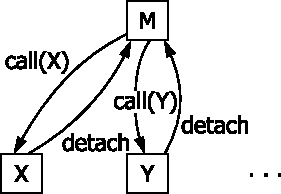
\includegraphics[width=.3\textwidth]{chap3/fig1}
\end{center}

\noindent
另一种方式是把决策“分散”出去，让对象自己通过 resume 操作决定接下来执行哪个对象。

\begin{center}
	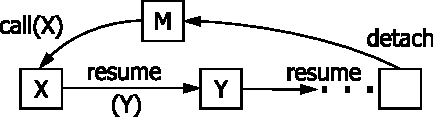
\includegraphics[width=.44\textwidth]{chap3/fig2}
\end{center}

\noindent
由 $X$ 执行的 resume$(Y)$ 操作，相当于先退出 $X$（通过 detach），再执行 call$(Y)$，从而绕过 $M$。把控制权交还给 $M$ 的责任也随之转移给 $Y$。

一个典型协程对象的经历，可以概括如下：

\begin{enumerate}[wide, nosep, label=(\arabic*)]
	\item 生成时，对象开始执行其类体中的操作；此时称它\textit{正在运行}，并\textit{附着}于创建它的对象生成器（所在的程序块实例）。
	\item 对象执行一条 \textit{detach} 语句，把控制权交还给生成对象的位置。此时称对象已经脱离，但尚未终止。detach 语句在对象的主体中留下一个标记，指出以后继续执行其操作的位置。这个标记位于该对象最近一次执行的 detach 语句末尾。
	\item 当执行 call 或 resume 语句，并通过引用参数指定该对象时，控制权便返回该对象。如果使用 call，它就\textit{重新附着}于\textit{调用它的}程序块实例；如果使用 resume，则重新附着于最初的调用者。此后，对象可以再次通过 detach 或 resume 暂时交出控制权；在这种情况下，它再次成为脱离状态。
	\item 或者，对象可以通过执行到自身的 \textbf{end}，最终交出控制权，这具有与 detach 相同的效果。但此时称它已经\textit{终止}，不能再通过 call 或 resume 重新激活。不过，它仍作为一项数据存在，可以通过远程标识来引用其属性，包括过程和函数属性，就像前面直方图的情形一样。
\end{enumerate}

\textit{注}。detach 操作表示从一个\textit{对象}中作协程退出，它只允许出现在对象的文本内部，即类体的文本内部。如果在子程序块或过程体中执行 detach，它仍表示退出在文本上包含它的最内层对象。对于 resume 指令（其中也包含协程退出），
情况也一样。然而，call 指令可以用在程序中的任何位置。

\subsection{文本转换}

我们用 Conway 提出的一个问题 [\hyperref[ref:7]{7}] 来说明协程的协作。需要从卡片中读入一段文本，再用行式打印机打印出来。每张卡片含 80 个字符，而打印机每行打印 125 个字符。目标是让每个输出行尽可能装满字符，卡片之间的过渡只通过额外插入一个空格来标记。文本中任何连续的两个星号都要替换成 ``$\uparrow$''。文本末尾用一个称为 ``end'' 的特殊字符标记。

假定已有一个协程 ``incard''，每次恢复执行时，它都从进卡槽中的下一张卡片读取字符，填入数组 $C[1 : 80]$，然后把卡片送到收卡槽。此外，已有一个协程 ``lineout''，每次恢复执行时，它都把数组 $L[1 : 125]$ 中的字符打印到纸上的下一行，然后换行。

这项任务由三个协程完成，分别通过以下引用来识别：

\quad \textbf{ref} disassembler, squasher, assembler;

disassembler 通过 $C$ 输入一张卡片，在卡片之间插入空格，再通过 $c1$ 把字符逐个输出给 squasher。squasher 完成双星号的转换，并通过 $c2$ 把字符逐个输出给 assembler。assembler 把字符组装成行并输出；它还负责检测 ``end'' 字符并作相应处理。

所需的类声明如下：

\quad \textbf{class} pass 1;

\quad \textbf{begin} detach;

\quad \quad \textbf{while true do}

\quad \quad \quad \textbf{begin integer} $i$; resume$($incard$)$;

\quad \quad \quad \quad \textbf{for} $i\coloneq 1$ \textbf{step} 1 \textbf{until} 80 \textbf{do}

\quad \quad \quad \quad \quad \textbf{begin} $c1\coloneq C[i]$; resume$($squasher$)$ \textbf{end};

\quad \quad \quad \quad $c1\coloneq$ blank; resume$($squasher$)$

\quad \quad \quad \textbf{end} infinite loop;

\quad \textbf{end} pass 1;

\quad \textbf{class} pass 2;

\quad \textbf{begin} detach;

\quad \quad \textbf{while true do}

\quad \quad \quad \textbf{begin if} $c1 =$ ``*'' \textbf{then}

\quad \quad \quad \quad \textbf{begin} resume$($disassembler$)$;

\quad \quad \quad \quad \quad \textbf{if} $c1 =$ ``*'' \textbf{then} c2: = ``$\uparrow$''

\quad \quad \quad \quad \quad \textbf{else begin} $c2 \coloneq$ ``*''; resume$($assembler$)$;

\quad \quad \quad \quad \quad \quad $c2\coloneq c1$

\quad \quad \quad \quad \quad \textbf{end};

\quad \quad \quad \quad \textbf{end}

\quad \quad \quad \textbf{else} $c2\coloneq c1$;

\quad \quad \quad resume (assembler); resume (disassembler)

\quad \textbf{end} infinite loop;

\quad \textbf{end} pass 2;

\quad \textbf{class} pass 3;

\quad \textbf{begin} detach;

\quad \quad \textbf{while true do}

\quad \quad \quad \textbf{begin integer} $i$;

\quad \quad \quad \quad \textbf{for} $i\coloneq 1$ \textbf{step} $1$ \textbf{until} 125 \textbf{do}

\quad \quad \quad \quad \quad \textbf{begin} $L[i] \coloneq c2$;

\quad \quad \quad \quad \quad \quad \textbf{if} $c2 =$ ``end'' \textbf{then}

\quad \quad \quad \quad \quad \quad \textbf{begin for} $i\coloneq i + 1$ \textbf{step} 1 \textbf{until} 125 \textbf{do}

\quad \quad \quad \quad \quad \quad \quad $L[i] \coloneq$ blank;

\quad \quad \quad \quad \quad \quad \quad resume$($lineout$)$;

\quad \quad \quad \quad \quad \quad \quad detach; \textbf{comment} 返回主程序;

\quad \quad \quad \quad \quad \quad \textbf{end}

\quad \quad \quad \quad \quad \quad \textbf{else} resume$($squasher$)$

\quad \quad \quad \quad \quad \quad \textbf{end} of this line;

\quad \quad \quad \quad resume$($lineout$)$

\quad \quad \quad \textbf{end} infinite loop

\quad \textbf{end} pass 3;

主程序为每一遍处理生成一个实例。每个实例都立即从主程序脱离。调用 disassembler，便启动了整个协程系统。检测到任务结束时，assembler 执行 detach 指令。由于 assembler 是通过来自 disassembler 的 resume 指令（间接地）取得控制权的，它执行 detach 的效果，与 disassembler 执行 detach 的效果相同：控制权返回主程序，而主程序随即终止。

主程序如下：

\quad \textbf{begin} disassembler: $-$ \textbf{new} pass 1;

\quad \quad squasher: $-$ \textbf{new} pass 2;

\quad \quad assembler: $-$ \textbf{new} pass 3;

\quad \quad call$($disassembler$)$;

\quad \textbf{end}

五个协程与主程序之间的关系，可以用图表示：
\begin{center}
	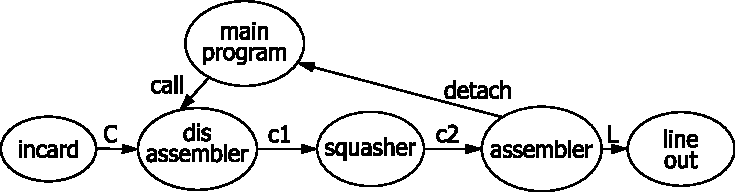
\includegraphics[width=.7\textwidth]{chap3/fig3}
\end{center}

\noindent
水平箭头表示 resume$/$resume 关系。箭头方向对应信息流的方向，箭头旁标注的变量名则指出用于保存所传递信息的变量。

在这个例子中，每个类始终只打算拥有一个对象，因此，完整的类$/$生成$/$引用机制显得过于繁复。其不便之处在于，必须为类和它唯一的对象分别取名（例如 pass 1 和 disassembler）。此外，在实现中，理应可以利用这种特殊情形，同时节省空间和时间。但 SIMULA 67 并没有提供实现这一点的手段。

\subsection{排列生成器}

我们希望定义一个 ``permuter'' 类，表示排列的概念。该类的对象应能生成从 1 到 $n$ 的整数的所有排列，其中 $n$ 是类的一个参数。类的一个属性是一个 \textbf{integer array} $p[1:n]$；生成该类对象时，它初始化为 $(1, 2, \dots, n)$（表示恒等排列）。此后，每次调用对象
都会使数组 $p$ 取一个新的排列作为值。当所有排列都生成完毕时，属性

\quad \textbf{Boolean} more;

\noindent
（初值为 true）会被赋予 \textbf{false}，对象也随之终止。

如果程序要考察 $N$ 个数的所有排列，其典型结构如下：

\quad \textbf{ref} $($permuter$)P$;

\quad $P$: $-$ \textbf{new} permuter$(N)$;

\quad \textbf{while} $P$.more \textbf{do}

\quad \quad \textbf{begin}\dots 考察 $P.p$\dots; call$(P)$ \textbf{end};

\noindent
permuter 类采用半协程结构，每次更新 $p$ 后，都会执行一条 detach 指令：

\quad \textbf{class} permuter$(n)$; \textbf{integer} $n$;

\quad \quad \textbf{begin integer array} $p[1:n]$;

\quad \quad \quad \textbf{Boolean} more;

\quad \quad \quad \textbf{integer} $q$;

\quad \quad \quad \textbf{for} $q\coloneq 1$ \textbf{step} 1 \textbf{until} $n$ \textbf{do} $p[q]\coloneq q$;

\quad \quad \quad more $\coloneq$ \textbf{true};

\tabto*{3.3em} \dots 生成 $p$ 的所有排列，

\quad \quad \quad 每生成一个排列就执行一次 ``detach''\dots;

\quad \quad \quad more $\coloneq$ \textbf{false}

\quad \quad \textbf{end}

接下来还要寻找一个算法，生成 $p[1]$、$p[2]$、\dots、$p[n]$ 的所有排列，并将它们恢复到原来的状态。这个算法可以采用递归结构。假定我们已经知道如何生成下面这些数的\textit{所有}排列：

\quad $p[1], p[2], \dots, p[k - 1],$

\noindent
并最终把它们恢复到原来的状态。完成这件事的过程调用是

\quad permute$(k - 1)$.

\noindent
现在，只需用这个过程，把原来的 $k$ 个数中每个由 $k - 1$ 个数组成的\textit{组合}进行全排列。因此，必须调用 permute$(k - 1)$ 共 $k$ 次；每次调用时，$1 \leqslant i \leqslant k$ 范围内的 $p[i]$ 中，恰有一个必须排除在操作之外。一个好办法是把它的值与 $p[k]$ 的值交换，因为 permute$(k - 1)$ 不会触及 $p[k]$。要保证 $k$ 个值各被排除恰好一次，可以利用我们所作的假定：过程返回时，给定序列保持不变。这样，依次交换 $p[1]$ 与 $p[k]$、$p[2]$ 与 $p[k]$、\dots、$p[k - 1]$ 与 $p[k]$，就能使每个值都恰好一次被赋给 $p[k]$。由此得到下面的核心程序：

\quad \textbf{integer} $i$;

\quad permute$(k - 1)$;

\quad \textbf{for} $i\coloneq 1$ \textbf{step} 1 \textbf{until} $k - 1$ \textbf{do}

\quad \quad \textbf{begin} swap$(p[i]$, $p[k])$; permute$(k - 1)$ \textbf{end};

\noindent
假定 permute$(k - 1)$ 不改变 p，这段核心程序的净效果，是把元素 $p[1]$、$p[2]$、\dots、$p[k]$ 向右循环移动一位。下面的例子可以说明这一点：

\quad 原始状态：\tabto*{12em}  1 2 3 4 5

\quad 执行 swap$(p[1], p[5])$ 后：\tabto*{12em} 5 2 3 4 1

\quad 执行 swap$(p[2], p[5])$ 后：\tabto*{12em}  5 1 3 4 2

\quad 执行 swap$(p[3], p[5])$ 后：\tabto*{12em}  5 1 2 4 3

\quad 执行 swap$(p[4], p[5])$ 后：\tabto*{12em}  5 1 2 3 4

\noindent
由于整个操作结束后必须使数组 $p$ 恢复原状，因此右循环移位之后，还须作一次补偿性的左循环移位。

\quad $q\coloneq p[1];$

\quad \textbf{for} $i\coloneq 1$ \textbf{step} 1 \textbf{until} $k - 1$ \textbf{do} $p[i]\coloneq p[i + 1]$;

\quad $p[k]: = q$

\noindent
最后，需要确定 $k = 1$ 时应执行什么操作。回想一下，这个过程的目的在于

\hangindent=1.9\parindent\quad “生成 $k$ 个对象的所有排列，每生成一个排列就执行一条 detach 指令”。

\noindent
一个数只有一种排列，就是它自身，因此只需执行一条 detach 指令。

permute 过程必须写成 permuter 类的一个属性，使它执行的 detach 针对相应的对象。现在可以声明整个类：

\quad \textbf{class} permuter$(n)$; \textbf{integer} $n$;

\quad \textbf{begin integer array} $p[1:n]$; \textbf{integer} $q$; \textbf{Boolean} more;

\quad \quad \textbf{procedure} permute$(k)$; \textbf{integer} $k$;

\quad \quad \textbf{if} $k = 1$ \textbf{then} detach \textbf{else}

\quad \quad \textbf{begin integer} $i$; permute$(k - 1)$;

\quad \quad \quad \textbf{for} $i\coloneq 1$ \textbf{step} 1 \textbf{until} $k - 1$ \textbf{do}

\quad \quad \quad \textbf{begin} $q\coloneq p[i]$; $p[i]\coloneq p[k]$;

\quad \quad \quad \quad $p[k]\coloneq q$; permute$(k - 1)$

\quad \quad \quad \textbf{end};

\quad \quad \quad $q\coloneq p[1]$;

\quad \quad \quad \textbf{for} $i\coloneq 1$ \textbf{step} 1 \textbf{until} $k - 1$ \textbf{do} $p[i] \coloneq p[i + 1]$;

\quad \quad \quad $p[k]\coloneq q$

\quad \quad \textbf{end} of permute;

\quad \quad \textbf{for} $q\coloneq 1$ \textbf{step} 1 \textbf{until} $n$ \textbf{do} $p[q] \coloneq q$;

\quad \quad \quad more $\coloneq$ \textbf{true}; permute$(n)$; more $\coloneq$ \textbf{false}

\quad \textbf{end} of permuter;

\textit{注}。permute 过程实例所执行的 detach，\textit{不是}退出该过程实例，也不会把控制权交还给调用该过程的位置。它是从整个对象（包括整个递归过程）中作一次暂时退出，把控制权交还给生成或调用该对象的主程序。因此，下一次调用对象时，递归过程会从上次暂停的位置原样继续。

规定（假定）permute 过程应使序列保持不变，实际上完全是一种任意的选择。请读者用同样的交换策略编写一个过程，使它返回时各个数的顺序恰好反转，以此验证这一点。

\section[链表结构]{链表结构}

上面介绍的类声明和对象引用机制，
可以用来表示栈、树这样的递归数据结构，
甚至可以表示双向链表这样的循环结构。实现的方法是
把一个类的某些属性声明为引用，所引用的对象仍属于
这个类本身。

\subsection{二叉搜索树}

二叉树可以定义为

\quad 或者 \tabto*{5.35em}$($i$)$ \tabto*{7.35em}\textbf{none}

\tabto*{4em}或者 $($ii$)$ 一个节点，

\noindent
其中节点由以下部分组成：

\begin{enumerate}[wide, nosep, label=(\alph*)]
	\item 左分量，它是一棵树
	\item 右分量，它是一棵树
	\item val，它是一个整数。
\end{enumerate}

\noindent
可以把 val 分量看作与树的每个节点相关联的值。左右子树都为 \textbf{none} 的节点，是树的终端元素（叶节点）。

二叉搜索树是一种二叉树：它或者是 \textbf{none}，或者是一个节点，该节点的 val 介于左子树所有 val 与右子树所有 val 之间，而且左右子树本身也都是二叉搜索树。二叉搜索树的用途，是对于任意整数，都能快速访问 val 等于该整数的节点；同时，也能快速插入具有任意给定 val 的新节点。因此，表示二叉搜索树概念的类具有以下形式：

\quad \textbf{class} tree$($val$)$; \textbf{integer} val;

\quad \quad \textbf{begin ref} $($tree$)$ left, right;

\quad \quad \quad \textbf{procedure} insert$(x)$; \textbf{integer} $x$;

\quad \quad \quad \quad \dots

\quad \quad \quad \textbf{ref} $($tree$)$ \textbf{procedure} find$(x)$; \textbf{integer} $x$;

\quad \quad \quad \quad \dots

\quad \quad \textbf{end} of tree;

这两个过程组件的主体，都是很简单的递归过程，与树的递归结构相对应：

\quad insert: \textbf{if} $x <$ val \textbf{then}

\quad \quad \textbf{begin if} left $==$ \textbf{none then} left: $-$ \textbf{new} tree$(x)$ \textbf{else} left.insert$(x)$

\quad \quad \textbf{end}

\quad \textbf{else if} right $==$ \textbf{none then} right: $-$ \textbf{new} tree$(x)$ \textbf{else} right.insert$(x)$;
\smallskip

\quad find: \textbf{if} $x =$ val \textbf{then this} tree

\quad \textbf{else if} $x <$ val \textbf{then} $($\textbf{if} left $==$ \textbf{none then none else} left.find$(x))$

\quad \textbf{else if} right $==$ \textbf{none then none else} right.find$(x);$

\noindent
在 ``find'' 的主体中，出现了表达式

\quad \textbf{this} tree

\noindent
它返回对当前节点的引用，也就是拥有 find 属性这个具体实例的节点。例如，如果用下面的函数指示符调用 $X$ 的 find 过程，

\quad $X.$find$(x)$

\noindent
并且 $X.\text{val} = x$，那么函数结果就是 $X$ 自身的引用值。

对二叉搜索树，另一项有意义的操作是按升序扫描其全部值。这项操作可以由一个“生产数据”的半协程实现；每次调用时，它把树中下一个较大节点值赋给如下属性：

\quad \textbf{integer} current;

\noindent
扫描完整棵树后，属性 current 将取最大整数值。

扫描可以通过一个递归的过程属性完成，它是相应协程实例的局部过程。

\quad \textbf{class} scanner$(X)$; \textbf{ref} $($tree$)\ X$;

\quad \quad \textbf{begin integer} current;

\quad \quad \quad \textbf{procedure} traverse$(X)$; \textbf{ref} $($tree$)\ X$;

\quad \quad \quad \quad \textbf{if} $X =/=$ \textbf{none then}

\quad \quad \quad \quad \quad \textbf{begin} traverse$(X$.left$)$;

\quad \quad \quad \quad \quad \quad current $\coloneq X$.val;

\quad \quad \quad \quad \quad \quad detach;

\quad \quad \quad \quad \quad \quad traverse$(X$.right$)$

\quad \quad \quad \quad \quad \textbf{end} traverse;

\quad \quad \quad traverse$(X)$;

\quad \quad \quad current $\coloneq$ integer max

\quad \quad \textbf{end} scanner;

作为使用这些概念的例子，我们考虑合并几棵二叉搜索树中的值。这些树保存在一个数组中：

\quad \textbf{ref} $($tree$)$ \textbf{array} forest$[1: N]$;

\noindent
目标是按升序输出这些值。为此，需要 $N$ 个扫描器，森林中的每棵树各配一个：

\quad \textbf{ref} $($scanner$)$ \textbf{array} trav$[1: N]$;

\quad \textbf{for} $i\coloneq 1$ \textbf{step} 1 \textbf{until} $N$ \textbf{do} trav$[i]$: $-$ \textbf{new} scanner$($forest$[i]);$

\noindent
此时，每个扫描器都已将自己的最小 val 赋给自己的 current，并脱离了调用程序。接下来，只需找出 $N$ 个 current 的最小值并输出，然后再次调用对应的扫描器，产生它的下一个较大 val。当最小值成为最大整数值时，合并就完成了。

\quad \textbf{integer} $min,\ j,\ i$;

\quad min $\coloneq 0$;

\quad \textbf{while} min $<$ integer max \textbf{do}

\quad \quad \textbf{begin} min $\coloneq$ trav$[1]$.current; $j\coloneq 1$;

\quad \quad \quad \textbf{for} $i\coloneq 2$ \textbf{step} 1 \textbf{until} $N$ \textbf{do}

\quad \quad \quad \quad \textbf{if} min $>$ trav$[i]$.current \textbf{then}

\quad \quad \quad \quad \quad \textbf{begin} min $\coloneq$ trav$[i]$.current;

\quad \quad \quad \quad \quad \quad $j\coloneq i$

\quad \quad \quad \quad \quad \textbf{end} 搜索最小的 current;

\quad \quad \quad \textbf{if} min $<$ integer max \textbf{then}

\quad \quad \quad \quad \textbf{begin} output$($min$)$;

\quad \quad \quad \quad \quad call$($trav$[j])$

\quad \quad \quad \quad \textbf{end}

\quad \quad \textbf{end} 合并过程;

\subsection{语法分析器}

作为一个更为完整的链表处理例子，我们来看通用的表驱动上下文无关语法分析器。这里采用自顶向下的回溯算法，在文法不含左递归的前提下，它能够发现所有可能的分析（文法有歧义时会有不止一种分析）。符号串用一条“带”来表示，它具有以下操作。

\quad \textbf{procedure} move right; \dots;

\quad \textbf{procedure} move left; \dots;

\quad \textbf{integer procedure} symbol; \dots;

\noindent
``move'' 操作把读头向右或向左移动一个符号。``symbol'' 过程读出读头下的符号，并按照一一映射把它转换为整数。

给定函数 ``meta''，用来判定某个整数是否表示元符号（meta-symbol）。

\quad \textbf{Boolean procedure} meta$(S)$; \textbf{integer} $S$; \dots;

\noindent
为简单起见，用一个三维数组 $G$ 表示文法：

\quad \textbf{integer array} $G[\dots, \dots, \dots]$;

\noindent
其中 $G[i, j, k]$ 保存整数 $i$ 所表示元符号的第 $j$ 个候选右部中的第 $k$ 个符号。还有一个

\quad \textbf{integer array} $jm[\dots]$;

\noindent
其中 $jm[i]$ 是给定元符号的候选右部数目。每个右部后都接上一个不属于该文法词汇的特殊符号 ``$\perp$''。如果某个语法类别的一项候选定义是 $\langle$empty$\rangle$，就仅用这个符号来表示它。

例如，考虑下面这个简单的上下文无关文法，它描述算术表达式的一个子类：

\begin{enumerate}[wide, nosep, label=(\arabic*)]
	\item $\langle$exp$\rangle ::= \langle$term$\rangle\ |\ \langle$term$\rangle\langle$addop$\rangle\langle$exp$\rangle$
	\item $\langle$term$\rangle ::= \langle$primary$\rangle\ |\ \langle$primary$\rangle\langle$mulop$\rangle\langle$term$\rangle$
	\item $\langle$primary$\rangle ::= \langle$constant$\rangle\ |\ \langle$variable$\rangle\ |\ (\langle$exp$\rangle)$
	\item $\langle$addop$\rangle ::= +\ |\ -$
	\item $\langle$mulop$\rangle ::= \times\ |\ /$
	\item $\langle$constant$\rangle ::= 1\ |\ 2\ |\ 3\ |\ 4\ |\ 5\ |\ 6\ |\ 7\ |\ 8\ |\ 9\ |\ 0$
	\item $\langle$variable$\rangle ::= I\ |\ J\ |\ K\ |\ L\ |\ M\ |\ N$
\end{enumerate}

\noindent
这里有七个元符号，可以赋予它们从 1 到 7 的整数值。22 个终结符可以赋予从 8 到 29 的值，而终止符 ``$\perp$'' 可以赋值为 0。

现在，表示这个文法的数组 $G$ 可以声明为：

\quad \textbf{integer array} $G[1:7, 1:10, 1:4]$

\noindent
这个数组的第一个平面取值如下：

\quad $G[1,\ .,\ .] = 2,\ 0,\ 0,\ 0$\tabto*{12em} 第一个候选右部

\tabto*{7.4em}$2,\ 4,\ 1,\ 0$\tabto*{12em} 第二个候选右部

\tabto*{7.4em}$0,\ 0,\ 0,\ 0$\tabto*{12em} 其余 8 行

\tabto*{7.4em}\quad\dots\tabto*{12em} 无关紧要。

\tabto*{7.4em}$0,\ 0,\ 0,\ 0$

\noindent
还请注意：

\quad $jm[1] = 2,\ jm[6] = 10$

\quad meta$(1) =$ meta$(7) =$ \textbf{true}

\quad meta$(8) =$ meta$(29) =$ \textbf{false}

把文本的第一个符号置于读头下，再生成语法分析器的一个实例，我们希望得到的结果是：产生一棵完整的语法树来表示这段文本；读头停在已分析文本最后一个字符\textit{之后}的字符上；变量 ``good'' 被置为 \textbf{true}。以后再调用同一实例，则产生表示其他分析方式的语法树。当再没有其他分析方式时，输入文本退回起点，变量 good 被置为 \textbf{false}。如果输入文本含有语法错误，那么第一次生成实例时就会出现这种情况。

请注意，分析器会找出文本任意前缀的所有成功分析。

每次调用分析器所输出的语法树，都为文本中识别出的每个短语包含一个节点。每个短语具有以下属性：

\quad \textbf{integer} $i$：表示短语的语法类别

\quad \textbf{integer} $j$：表示它属于该类别的哪一个候选项

\quad \textbf{ref} $($phrase$)$ sub：引用给定短语的最后一个子短语

\hangindent=3.2\parindent\quad \textbf{ref} $($phrase$)$ left：引用同一分析层次上紧邻该短语左侧的短语。任何短语的第一个子短语，其 left 都为 \textbf{none}。

\noindent
因此，表达式
$$
M\times N + 7
$$

\noindent
应产生图 \ref{fig:syntax-analyzer-1} 所示形式的树。

语法分析器将采用递归结构，由一个短语对象类构成；每个短语对象都会对单个短语，重现整个分析器应具有的行为。

短语对象接收一个元符号 $i$ 和一个左邻短语作为参数，负责生成给定语法类别的所有可能语法树，使之匹配当前符号起及其右侧的一段文本。每次成功分析后，输入文本都前进到\textit{不}属于该次分析的第一个符号处。当所有可能的分析都完成时，带退回进入该短语之前的位置，全局变量 good 被置为 \textbf{false}，短语对象随即终止。

现在可以概述 phrase 类的一般结构：

\quad \textbf{class} phrase$(i,$ left$)$; \textbf{integer} $i$; \textbf{ref} $($phrase$)$ left;

\quad \quad \textbf{begin integer} $j$; \textbf{ref} $($phrase$)$ sub;

\quad \quad \quad \textbf{for} $j\coloneq 1$ \textbf{step} 1 \textbf{until} $jm[i]$ \textbf{do}

\quad \quad \quad \quad \dots 用所有可能的方式将余下的文本

\quad \quad \quad \quad 与类别 $i$ 的第 $j$ 个候选项匹配，

\quad \quad \quad \quad 每次匹配成功后执行一次 detach \dots;

\quad \quad \quad good $\coloneq$ \textbf{false}

\quad \textbf{end} of phrase;

假定某对象已成功匹配了给定元符号 $(i)$ 的某个候选右部 $(j)$ 的前 $k - 1(k > 0)$ 个符号。现在编写一段程序，以所有可能的方式，将第 $k$ 个符号与输入匹配。假定语句 ``match remainder''（匹配余下部分）会以所有可能的方式，把右部尚余的部分（如果有）与输入匹配，并且该语句不改变读头位置，也不改变已经构造出的语法树部分。对于未能识别出（另一个）短语的对象，我们也作出后一项假定。

\begin{enumerate}[nosep, label=\arabic*.]
	\item \textbf{begin integer} $g$; $g\coloneq G[i, j, k]$;
	\item \label{en:comment-label-2}
	\quad \textbf{if} $g =$ ``$\perp$'' \textbf{then begin} good $\coloneq$ \textbf{true}; detach \textbf{end}
	
	\item \quad \textbf{else if} $g =$ symbol \textbf{then}
	
	\item \label{en:comment-label-4}
	\quad \textbf{begin} move right; match remainder; move left \textbf{end}
	
	\item \quad \textbf{else if} meta$(g)$ \textbf{then}
	
	\item \label{en:comment-label-6}
	\quad \textbf{begin} sub: $-$ \textbf{new} phrase$(g,$ sub$)$;
	\item \quad \quad \textbf{while} good \textbf{do}
	
	\item \label{en:comment-label-8}
	\quad \quad \textbf{begin} match remainder; call$($sub$)$ \textbf{end};
	
	\item \label{en:comment-label-9}
	\quad \quad sub: $-$ sub.left
	
	\item \quad \quad \textbf{end}
	\item \quad \textbf{end}
\end{enumerate}

\begin{figure}[h]
	\centering
	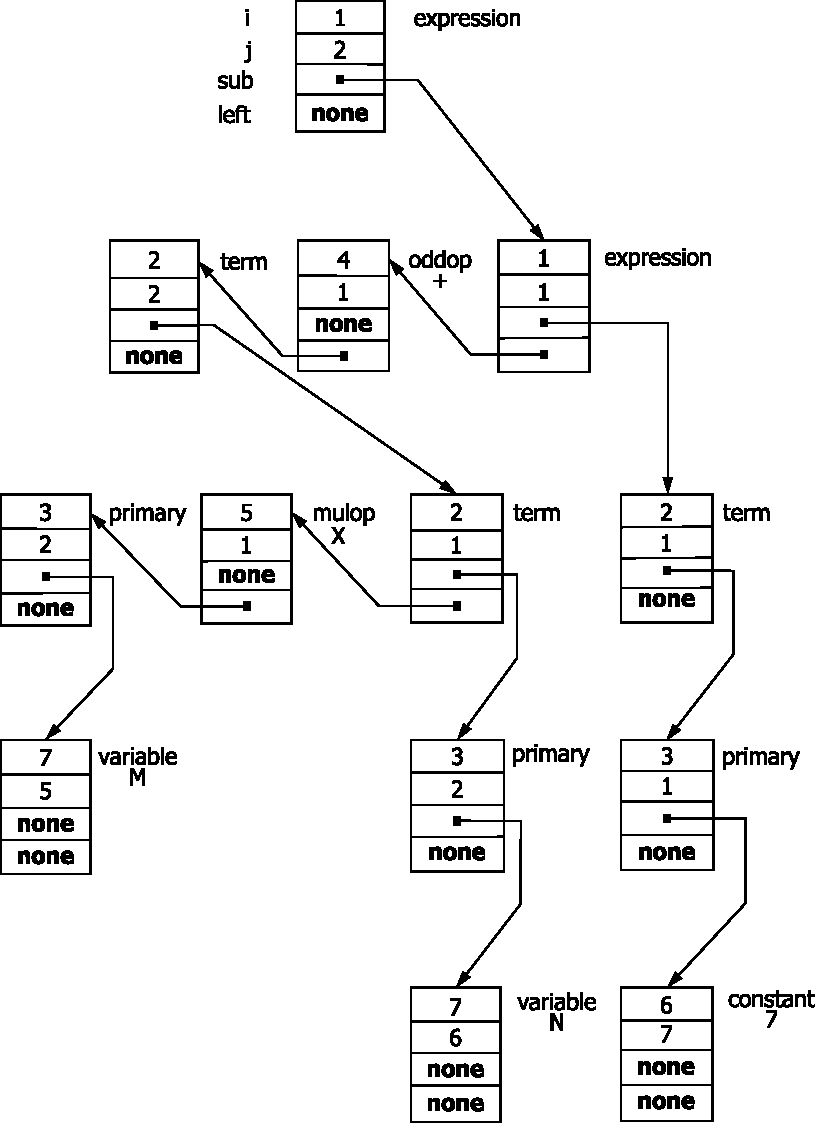
\includegraphics[width=.6\textwidth]{chap3/fig4}
	\caption{语法分析器的树形表示}
	\label{fig:syntax-analyzer-1}
\end{figure}

\noindent
\textit{说明}。

\begin{enumerate}[leftmargin=*, itemindent=2.2\parindent, nosep, label=第 \arabic* 行.]
	\item 为简便起见，把编号为 $j$ 的右部的第 $k$ 个符号称为 $g$。
	\item 如果 $g$ 是终止符，整个右部就已经成功地与输入匹配。对象向其主控程序报告。第 \hyperref[en:comment-label-2]{2} 行不改变语法树或读头位置。

	\setcounter{enumi}{3}
	\item 既然符号已匹配，对象就把读头移到下一个符号。在用所有可能的方式匹配余下部分之后，
	对象恢复读头的位置。因此，根据假定，第 \hyperref[en:comment-label-4]{4} 行的净效果为零。
	
	\setcounter{enumi}{5}
	\item 由于 $g$ 是元符号，生成一个新的 phrase 对象，识别语法类别 $g$ 的子短语。它成为新的最右子短语，其左邻短语是原来的最右子短语。
	
	\item 我们已假定，对象失败时会把 ``good'' 置为 \textbf{false}。
	
	\item 由于 ``good'' 为 \textbf{true}，已经识别出一个与 $g$ 匹配的子短语。在以所有可能的方式匹配余下部分之后，调用 ``sub''，识别下一个可能的子短语。由于我们要以所有可能的方式匹配 $g$，因此重复第 \hyperref[en:comment-label-8]{8} 行，直到子短语对象失败。
	
	\item 根据假定，失败的短语对象，其净效果为零。因此，第 \hyperref[en:comment-label-6]{6}\textendash\hyperref[en:comment-label-8]{8} 行的总效果，是在语法树上添加一个对象。第 \ref{en:comment-label-9} 行将语法树恢复到原来的状态。
\end{enumerate}

上述说明表明，上面的程序块会以所有可能的方式，匹配符号 $g$ 及其后元符号 $i$ 的第 $j$ 个右部的余下部分，而净效果为零。因此，这个程序块本身满足我们对 ``match remainder'' 语句作出的假定。由此可知，整个匹配算法可以用一个递归过程简洁地表达。下面的类声明描述了整个计算过程。

\quad \textbf{class} phrase$(i$, left$)$; \textbf{integer} $i$; \textbf{ref} $($phrase$)$ left;

\quad \textbf{begin integer} $j$; \textbf{ref} $($phrase$)$ sub;

\quad \quad \textbf{procedure} match$(k)$; \textbf{integer} $k$;

\quad \quad \textbf{begin integer} $g$; $g\coloneq G[i,j, k]$;

\quad \quad \quad \textbf{if} $g =$ ``$\perp$'' \textbf{then begin} good $\coloneq$ \textbf{true}; detach \textbf{end}

\quad \quad \quad \textbf{else if} $g =$ symbol \textbf{then}

\quad \quad \quad \textbf{begin} move right; match$(k + 1)$; move left \textbf{end}

\quad \quad \quad \textbf{else if} meta$(g)$ \textbf{then}

\quad \quad \quad \textbf{begin} sub: $-$ \textbf{new} phrase $(g$, sub$)$;

\quad \quad \quad \quad \textbf{while} good \textbf{do}

\quad \quad \quad \quad \textbf{begin} match$(k + 1)$; call$($sub$)$ \textbf{end};

\quad \quad \quad \quad \quad sub: $-$ sub.left

\quad \quad \quad \quad \textbf{end}

\quad \quad \textbf{end} of match;

\quad \quad \textbf{for} $j\coloneq 1$ \textbf{step} 1 \textbf{until} $jm[i]$ \textbf{do} match$(1);$

\quad \quad good $\coloneq$ \textbf{false}

\quad \textbf{end} of phrase

\noindent
主控程序可以采用以下结构：

\quad \textbf{ref} $($phrase$)$ tree;

\quad \dots

\quad tree: $-$ \textbf{new} phrase$($start, none$)$;

\quad \textbf{while} good \textbf{do begin} found: \dots; call$($tree$)$ \textbf{end};

\noindent
其中 ``start'' 表示文法的起始符号。到达标号 ``found'' 时，已经识别出一个句子，变量 ``tree'' 引用按上述方式表示的语法树。对每个节点，都可以通过远程标识，访问其相关元符号 $(i)$、候选右部编号 $(j)$，以及指向其他节点的链接 $($sub, left$)$，例如：

\quad tree.$i$, tree.sub.$j$, tree.sub.left.left.sub.

一般来说，我们必须预料到：从带上同一位置出发，不同成功尝试所匹配的串，长度可能不同。可以通过适当定义语言来避免这一点，使合法文本的任何真前缀都不再是合法文本。另一种办法是在整段文本之后加上一个不属于字母表的符号，比如 ``$\perp$''；此时主控程序可以采用以下结构：

\quad \textbf{ref} $($phrase$)$ parse; \textbf{Boolean} good;

\quad parse: $-$ \textbf{new} phrase $($start, \textbf{none}$)$;

\quad \textbf{while} good \textbf{do}

\quad \textbf{begin if} symbol $=$ ``$\perp$'' \textbf{then} 考察成功的语法分析结果;

\quad \quad call$($parse$)$

\quad \textbf{end}

phrase 类有一个显著特点：每次调用得到的结果都是一棵树，其节点由递归激活、尚未终止的 phrase 对象组成。每个 phrase 对象都有双重作用：既是供主控程序考察的语法树的一部分，又是一组局部变量，供其他 phrase 对象的递归激活使用。正是数据与过程之间的这种紧密联系，使算法能够表述得如此简单、简洁。

请注意，每个 phrase 对象都是一个独立栈的核心，这个栈保存它的局部过程 ``match'' 的递归激活。当某对象执行 detach，表示成功完成一次（子）语法分析时，它的栈达到暂时的最大深度：当前右部的每个符号各占一层，此外还有一层对应于执行 detach 的右部终止符 $\perp$。

因此，成功语法分析的整个动态上下文都被保留下来。再次调用对象以生成另一种分析时，会进行回溯，在此过程中，该对象的 ``match'' 栈逐层缩减。在与右部某个元符号对应的层次，match 过程调用相应的 phrase 对象，生成另一种子分析（第 \hyperref[en:comment-label-8]{8} 行），如此继续。（可联想卓别林《大独裁者》中那一排军官。）

\section{程序串接}

前面几节已经说明，\textit{类}机制可以通过规定数据结构并定义其上的操作，对某些简单概念建模。本节将提出一种方法，在较简单概念的基础上构造更复杂的概念。这使我们能够建立概念的层次结构：复杂概念从属于定义它所依据的那些较简单概念。这种结构技术提供了一种将程序各组成部分结合起来的新方法，称为\textit{串接}（concatenation）。

串接是在两个类 $A$ 与 $B$ 之间，或者在类 $A$ 与程序块 $C$ 之间定义的操作，其结果是一个新的类或程序块。串接包括合并两个组件的属性，并组合它们的动作。串接后对象的形式参数，由第一个组件的形式参数接上第二个组件的形式参数构成；说明部分、声明和语句（如果有）也按同样的方式连接。

在类 $B$ 的声明前加上第一个组件 $A$ 的名字作为前缀，就定义了串接后的类 $B$：

\quad $A$ \textbf{class} $B(b_1, b_2, \dots)$; \dots $b$ 参数的说明;

\quad\quad \textbf{begin}\dots $B$ 的属性\dots; \dots $B$ 的动作\dots \textbf{end}

\noindent
假定类 $A$ 已定义如下：

\quad \textbf{class} $A(a_1, a_2 , \dots)$; \dots $a$ 参数的说明\dots;

\quad \quad \textbf{begin}\quad $A$ 的属性\dots; \dots $A$ 的动作\dots \textbf{end}.

根据串接规则，类 $B$ 的上述带前缀声明
所产生的效果，等同于不带前缀的如下声明：

\quad \textbf{class} $B(a_1, a_2, \dots, b_1, b_2, \dots)$; \dots $a$ 参数的说明\dots

\quad \quad \quad $b$ 参数的说明\dots;

\quad \quad \textbf{begin}\dots $A$ 的属性\dots; \dots $B$ 的属性\dots;

\tabto*{5.9em}\dots $A$ 的语句\dots; \dots $B$ 的语句\dots \textbf{end};

\textit{注}。如果 $A$ 的某些局部标识符与 $B$ 的局部标识符相同，就通过系统地更改 $B$ 的标识符来消除名字冲突。程序块也可以用类标识符作前缀：

\quad $A$ \textbf{begin} 声明\dots; \dots 语句 \textbf{end},

\noindent
其效果与上面的说明相似，只是串接的结果是程序块，而不是类。（如果类 $A$ 有参数，前缀必须包含实际参数部分。）为程序块添加前缀后，在该程序块内部就可以使用 $A$ 的类声明中定义的过程库及相关数据（甚至包括类）。

同一个类可以作为多个不同串接类的前缀。例如，假定程序要处理卡车、公共汽车和私家车。这是三个独立的类，各有自己的属性。但因为它们都是车辆，有些属性（例如牌照号码）是三者共有的。车辆是一个更一般的概念，可以将它单独声明：

\quad \textbf{class} vehicle$($license no$)$; \textbf{integer} license no; \dots;

\noindent
现在，这个类就可以在其余类声明中用作前缀。

\quad vehicle \textbf{class} truck (load); \textbf{real} load; \dots;

\quad vehicle \textbf{class} bus (seating); \textbf{integer} seating; \dots;

\quad vehicle \textbf{class} car; \dots;

属于带前缀类的对象，是一个复合对象；\textit{除了}前缀部分定义的属性和操作，它还有一些额外的属性和操作。因此，truck 对象具有 license no 和 load，bus 对象具有 license no 和 seating。把 ``truck''、``bus'' 和 ``car'' 视为 vehicle 类的\textit{子类}是合理的；子类的任何对象也都属于前缀类 ``vehicle''。

引用变量可以用前缀类或串接后的类来限定。如果用前缀类限定，它就可以指向\textit{任何}子类的对象；通过远程标识符，可以访问前缀类的任何属性，但不能访问子类新增的属性。用子类限定的引用，只能指向该子类的对象，不过可以通过远程标识符访问它的所有属性。因此，给定引用变量：

\quad \quad \textbf{ref} $($vehicle$)\ V$; \textbf{ref} $($bus$)\ B$;

\quad 下列远程标识符合法：

\quad \quad $V$.license no, $B$.license no, $B$.seating,

\quad 但 $V$.seating 不合法。

\noindent
由此可见，子类概念使对象引用具有有用的灵活性。“弱”限定允许引用较广范围的对象，但代价是不能通过远程访问取得子类中声明的属性。

把子类引用赋给以前缀类限定的引用变量 $($例如 $V$: $-\ B)$，始终合法，而且可以在编译时确认。然而，反方向的赋值 $($例如 $B$: $-\ V)$，如果所引用对象实际上不属于所期望的子类（bus），就会产生错误，而这种错误只能在运行时检测。

\subsection{二叉搜索树}

假定我们要建立一棵二叉搜索树，保存库存货品的信息。树的每个节点不仅要包含 val（表示货品编号），还要包含现有库存量、价格、再订货点等其他信息。最简单的实现办法，是用 tree 类作 ``stock item'' 类的前缀，再声明所需的额外属性，例如：

\quad tree \textbf{class} stock item;

\quad \quad \textbf{begin integer} $qoh$, price, reorder point;

\quad \quad \quad \textbf{Boolean} ordered;

\quad \quad \quad \textbf{procedure} reduce;

\quad \quad \quad \quad \textbf{begin if} $qoh =$ reorder point \& $\neg$, ordered \textbf{then}

\quad \quad \quad \quad \quad 发出补货订单;

\quad \quad \quad \quad \quad $qoh \coloneq qoh -1$

\quad \quad \quad \quad \textbf{end} of remove;

\quad \quad \textbf{end} of stock item;

\subsection{双向链表}

利用串接技术，可以设计专门或主要用作其他类或程序块前缀的类。本小节给出 TWLIST 类的例子，它用于为程序块添加前缀，使程序块内部能够使用双向循环链表这个概念。这种链表具有一个\textit{链表头}，其中包含两个指针，一个指向链中的第一个元素，另一个指向最后一个元素。链中的每个\textit{链节点}（link）也必须包含两个指针：suc 指向链表中的后继（若无后继则指向链表头），pred 指向链表中的前驱（若无前驱则指向链表头）。空链表中，链表头的两个指针都指向它自身。

系统中的每个指针，都必须既能指向链表中的另一个链节点，也能指向链表头。因此，需要用一个同时涵盖链节点和链表头的类来限定这些指针，也就是 ``linkage'' 类；链节点与链表头都是它的子类。既然链表头和链节点都需要两个引用属性，就可以把 suc 和 pred 声明为前缀类 linkage 的属性。

双向链表这一个概念，由 linkage、link 和链表头这三个类共同表示。为了表明三者应作为一个概念一起理解，把它们的声明集中在同一个类声明 TWLIST 中。任何需要使用这个概念的程序块，都可以用 TWLIST 作前缀。在这样的程序块中，``link'' 类用于作其他类的前缀，那些类规定所存元素的性质；例如，如果货品存放在双向链表而不是二叉搜索树中，声明就是：

\quad link \textbf{class} stock; \dots 同前\dots;

现在，需要确定链表和链节点的一组基本操作。应当能通过下面的过程语句，把链节点 $I$ 从所属链表中移除：

\quad $I$.out;

\noindent
也应当能用下面的过程语句，把它重新插入某条链表，紧接在链节点 $J$ 之前：

\quad $I$.precede$(J)$;

\noindent
由于一个链节点至多属于一条链表，这项操作还应当先把 $I$ 从它原先所属的链表中移除。最后，还应当能用下面的过程语句，把一个链节点作为最后一个元素，插入以 $H$ 为头的链表：

\quad $I$.into$(H)$;

对于链表头 $H$，定义以下函数似乎很有用：

\quad $H$.empty,

\noindent
它检验链表是否为空；

\quad $H$.first

\noindent
它返回 $H$ 的第一个元素，若无元素则返回 \textbf{none}；以及

\quad $H$.last

\noindent
它返回 $H$ 的最后一个元素，若无元素则返回 \textbf{none}。

现在可以给出 TWLIST 类的声明：

\begin{enumerate}[nosep, label=\arabic*.]
	\item \textbf{class} TWLIST;
	\item \textbf{begin class} linkage; \textbf{begin ref} $($linkage$)$ suc, pred; \textbf{end};
	\item \quad linkage \textbf{class} link;
	\item \quad \textbf{begin procedure} out;
	\item \quad \quad \textbf{if} suc $=/=$ \textbf{none then}
	\item \quad \quad \textbf{begin} suc.pred: $-$ pred; pred.suc: $-$ suc;
	\item \quad \quad \quad suc: $-$ pred: $-$ \textbf{none}
	\item \quad \quad \textbf{end} of out;
	\item \quad \quad \textbf{procedure} precede$(x)$; \textbf{ref} $($linkage$)\ x$;
	\item \quad \quad \textbf{begin} out; suc: $-\ x$; pred: $-\ x$.pred;
	\item \quad \quad \quad suc.pred: $-$ pred.suc: $-$ \textbf{this} link
	\item \quad \quad \textbf{end} of precede;
	\item \quad \quad \textbf{procedure} into $(L)$; \textbf{ref} $($list$)\ L$;
	\item \quad \quad \quad precede$(L)$;
\end{enumerate}

\hangindent=2.9\parindent\quad \quad \quad \textbf{comment} link 对象的 suc 和 pred 应采用标准初值 \textbf{none}，表示不属于任何链表;

\begin{enumerate}[nosep, label=\arabic*.]
	\setcounter{enumi}{14}
	\item \quad \textbf{end} of link;
	\item \quad linkage \textbf{class} list;
	\item \quad \textbf{begin ref} $($link$)$ \textbf{procedure} first;
	\item \quad \quad \quad first: $-$ \textbf{if} empty \textbf{then none else} suc;
	\item \quad \quad \textbf{ref} $($link$)$ \textbf{procedure} last;
	\item \quad \quad \quad last: $-$ \textbf{if} empty \textbf{then none else} pred;
	\item \quad \quad \textbf{Boolean procedure} empty;
	\item \quad \quad \quad empty: $=$ suc $==$ \textbf{this} list;
	\item \quad \quad \quad suc: $-$ pred: $-$ \textbf{this} list
\end{enumerate}

\hangindent=3.6\parindent\quad \quad \quad \quad \textbf{comment} 链表头的 suc 和 pred 应初始化为表示空链表的状态;

\begin{enumerate}[nosep, label=\arabic*.]
	\setcounter{enumi}{23}

	\item \quad \textbf{end} of list;
	\item \textbf{end} of TWLIST;
\end{enumerate}

设 $P$ 是以 TWLIST 为前缀的\textit{任意}程序块实例，并且在其前缀部分之外，不对任何 linkage 对象的变量 suc 或 pred 作显式引用赋值。那么，下面的断言 \ref{en:twlist-1} 和 \ref{en:twlist-2}，在 $P$ 的整个生存期内都成立（限于控制权处于 TWLIST 主体文本之外的时刻）。

\begin{enumerate}[wide, nosep, label=(\arabic*)]
	\item \label{en:twlist-1}
	$P$ 中的任意 linkage 对象 $x$，或者不属于任何链表，此时 $x$.suc $== x$.pred $==$ \textbf{none}，且 $x \notin$ list；或者满足 $x\text{.suc.pred} == x\text{.pred.suc} == x$。
	
	由此可知，$P$ 中包含的所有链表都是循环链表。此外：
	
	\item \label{en:twlist-2}
	$P$ 中的每条循环链表，都恰好包含一个链表头，它是 ``list'' 类的对象。
\end{enumerate}

要确立这些断言，只需注意下面的每项操作
都保持它们成立，而 P 最初并不包含任何 linkage 对象。

\noindent
\textbf{new} \textit{link}（或 \textbf{new} $C$，其中 $C \subseteq$ linkage-list）生成一个 link 对象，它不属于任何链表（其 suc 和 pred 自动初始化为 \textbf{none}）。

\noindent
\textbf{new} \textit{list}（或 \textbf{new} $C$，其中 $C \subseteq$ list）生成一条“空”的循环链表，最初只包含生成的链表头，没有其他元素。

\noindent
以下假定 $x \in \text{link}$、$y$、$z \in \text{linkage}$，以及 $L \in \text{list}$。$x \leftrightarrow y$ 是 $x.\text{suc} == y$ \& $x == y$.pred 的简写。

\noindent
$x.out$：若 $z \leftrightarrow x \leftrightarrow y$，结果是 $z \leftrightarrow y$，而 $x$ 不再属于链表。（请注意，\ref{en:twlist-2} 与 $x \in \text{link}$ 共同推出 $x =/= y$、$z$。）若 $x$ 原本不属于任何链表，则什么也不做。

\noindent
$x.precede(y)$，其中 $x =/= y \land z \leftrightarrow y$。结果是 $x \leftrightarrow y$（若 $x =/= z$，还满足 $z \leftrightarrow x$）。如果 $x$ 原先属于某条链表，就先从该链表中移除 $x$。

\noindent
$x.into(L)$，其中 $z \leftrightarrow L$。结果是 $z \leftrightarrow x \leftrightarrow L$，这意味着 $x == L$. last。如果 $x$ 原先属于某条链表，就先从该链表中移除 $x$。

不满足上述假定的任何 out、precede 或 into 调用，要么在程序文本上就不合法，要么会因为无效的远程标识符，立即导致运行时错误并终止程序。例如，当 $x == y$ 或 $y$ 不属于任何链表时，操作 $x$.precede$(y)$ 会把 $x$.pred 置为 \textbf{none}。因此，precede 主体中的远程标识符 pred. suc 无效。请注意，$x$.into$(L)$ 是一种“更安全”的操作，因为 $x \in \text{link}$、$L \in \text{list}$ 意味着 $x =/= L$，且 $L.\text{pred} =/= \text{\textbf{none}}$。

只要不对任何变量 suc 或 pred 作显式赋值，断言 \ref{en:twlist-1} 与 \ref{en:twlist-2} 就保证了链表行为良好。因此，TWLIST 结构是一个可靠的“思维平台”：无论犯了什么程序设计错误，它在某种意义上都\textit{不会失效}。在 TWLIST 的基础上编程时，可以不去理会操作双向循环链表所涉及的链表处理细节。每个 list 对象都可以看作表示 link 对象的一个\textit{有序集合}，条件是任何 link 对象同一时刻至多属于一个这样的集合。这最后一点体现在 into 和 precede 过程的设计中。不过，显式使用属性 suc 和 pred，例如扫描链表时，使用者可能仍须记住：“最后”一个成员也有后继，“第一个”成员也有前驱，而二者都等于链表对象本身。另一种设计办法，是把下面的过程声明为 link 的属性，以隐藏这一细节。

\quad \textbf{ref} $($link$)$ \textbf{procedure} successor;

\quad \quad \textbf{inspect} suc \textbf{when} list \textbf{do} successor: $-$ \textbf{none}

\quad \quad \textbf{otherwise} successor: $-$ suc;

\quad \textbf{ref} $($link$)$ \textbf{procedure} predecessor;

\quad \quad \textbf{inspect} pred \textbf{when} list \textbf{do} predecessor: $-$ \textbf{none}

\quad \quad \textbf{otherwise} predecessor: $-$ pred;

请注意，结构

\quad \textbf{inspect} $r$ \textbf{when} $C$ \textbf{do}\dots

\noindent
使程序设计者能够检验 r 所引用的对象，是否属于它可能属于的某个子类 $C$。

\section{概念层次结构}

程序设计项目开始时，一端是一个\textit{问题}：它借助某些面向问题的概念，被或多或少地精确定义和理解；另一端是一种\textit{程序设计语言}：它可能是通用语言，提供一些面向机器的基本概念，我们希望这些概念已被精确定义并得到充分理解。两端之间存在一段\textit{概念距离}，必须用我们的程序将它衔接起来。可以把这段距离想象成竖直方向上的距离，而给定的程序设计语言就是地面。

跨越这种距离的困难在于，我们一次只能按顺序处理一个简单的子问题，而且并不总能事先知道这些是否是\textit{应该解决的问题}。

为了更好地克服这种困难，我们可以建造金字塔。与埃及的金字塔不同，我们的金字塔或者倒立着（自底向上构造），或者悬在空中（自顶向下构造）。这里采用的构造原则，最适合称为\textit{抽象}：我们专注于许多现象共有的特征，把与当前工作所处概念层次相距太远的特征\textit{舍去}。这样，就更有可能形成在后续阶段确实有用的概念。

自底向上构造时，我们从基本语言层次出发，构造能涵盖某个问题领域多种现象的抽象概念。自顶向下构造时 [\hyperref[ref:8]{8}, \hyperref[ref:9]{9}]，我们借助某些概念来表述给定问题的解；这些概念可以用多种方式实现（和解释），甚至可能尚未得到充分理解。无论哪种方式，构造系统都可以通过不断在金字塔上方或下方添加新层次来进行，直到最终跨越概念之间的距离。每一层都对应于理解上的一个概念层次。

例如，给定一个涉及排队现象的问题，可以把上一节的 TWLIST 作为自底向上构造的第一步。此后，在构造的其余部分，我们就可以自由地从动态操作对象有序集合的角度，
进行思考和表述。

各个概念层次，可以表示为类声明的一个\textit{前缀序列}。例如，可以构造一系列类声明，每个类都以前一个类作前缀：

\hfill\textbf{class} $C_1$; \dots;\hspace{14em}

\hfill $C_1$ \textbf{class} $C_2;$ \dots;\hspace{14em}

\tabto*{13em}\dots

\hfill $C_{n - 1}$ \textbf{class} $C_n$; \dots;\hspace{14em}

\noindent
序列 $C_1, C_2, \dots, C_{n-1}$ 称为 $C_n$ 的前缀序列。最外层前缀 $C_1$ 在地面层次上构造。其他每一层都建立在其下各层的基础上，因为它可以使用整个前缀序列的全部属性。借助这个语言机制，自底向上构造程序，就是按上述顺序，逐个规划并编写前缀序列中的类。最后，在整个序列之上，把程序本身写成一个带前缀的程序块：

\quad $C_n$ \textbf{begin}\textemdash{}\textbf{end}

\noindent
自顶向下策略则对应于按相反顺序，构造前缀序列的各个成员，包括带前缀的程序块。（SIMULA 67 还包含其他机制，可以方便自顶向下及混合方式的构造，这里不作讨论。）

一个构造良好的概念层次（自底向上），是一组定义明确、相互关联的概念，它们可以组合成更复杂的概念。这一层次可以为后续构造提供一个思维平台，使我们从地面向某个应用领域提升，也就是提供一种“应用语言”。预先构造的应用语言，能够缩短解决该领域许多问题时需要跨越的概念距离。这种平台是否有用，与它的稳固程度密切相关，也就是它能在多大程度上容忍、甚至防止误用。正如上一节所见，TWLIST 提供了一个格外稳固的思维平台；本节将在它的基础上，构造一种小巧而有用的应用语言，而这种语言又可以作为解决实际问题的平台。

\subsection{离散事件模拟}

模拟是一种方法，用于研究由相互作用的对象组成的大型系统的行为，并评估改变系统所产生的效果；在现实中以实验方式实施这些改变，代价可能过于高昂。模拟模型的研究对象可以是生产线、交通系统、计算机系统（硬件和软件）、由相互作用的个体组成的社会系统等等。大多数这样的系统，都具有以下共同现象。

\begin{enumerate}[wide, nosep, label=(\arabic*)]
	\item 各个过程\textit{并行}发生，在不规则的时间间隔后产生离散事件。
	\item 当对象必须等待一个目前正忙的服务者提供服务时，会出现\textit{排队}现象。
\end{enumerate}

为了表示并行发生的过程，并不需要把相应的程序组件在计算机上安排为多道程序；但必须允许程序暂时挂起自己，以后再从暂停处恢复。因此，模拟中的活动对象或“过程”，将由（半）协程来表示，在调度机制的控制下，以\textit{伪并行}方式运行。

例如，在作业车间模拟中，一份到来的订单会在车间引发一系列事件，以完成该订单。每份订单都可以视为一个过程，其活动是从一台机器移向下一台，请求并获得机器的服务。请求序列由订单的性质决定。如果所请求的机器空闲，就立即为订单提供服务，机器随之忙碌一段时间，长度等于服务时长。否则，订单就加入等待该机器空闲的订单队列。

实现模拟时间这个概念，首先要求每个过程都能访问一个保存当前时间的变量 ``time''；时间控制机制在适当的时刻增加它的值。请注意，这个变量的更新必须完全独立于模拟期间计算时间的流逝，因为计算机上耗时很长的动作，在现实世界中可能只需很短时间，反之亦然。就模拟时间而言，各个过程的活动阶段都必须是瞬时的；只有当所有参与的过程都处于非活动状态时，``time'' 才会前进。

因此，要模拟时间的流逝，一个模拟活动系统组件的过程，必须在给定的模拟时间间隔 $T$ 内交出控制权，并在 time 变量增加 $T$ 后重新激活。为此，过程将调用

\quad hold$(T)$.

例如，一份订单发现所需的机器已准备好为它服务时，需要用下面的语句，说明这项服务需要多长时间：

\quad hold$($service interval$)$;

\noindent
此时，这份订单变为非活动状态，直到所有本应在 time $+$ service interval \textit{之前}重新激活的其他订单，都已重新激活并再次交出控制权。到这时，给定订单重新激活，就会发现它的 time 已增加到相应的值。

过程处于暂停等待期间，必须把其重新激活的时间记录为自身的一个属性。因此，直接使用过程自身的 time 属性来记录，会很方便。

按指定时间间隔暂停的方法，只适用于过程知道距离它下一次“事件”还要等多久的情形。但有时，它需要等待另一个过程中的某个事件发生。例如，一份订单发现所需机器正忙，就必须加入队列，等待机器空闲；而订单释放机器时，必须激活队列中的第一份其他订单（如果队列非空）。因此，还需要两个过程：

\quad wait$(Q)$,

\quad 以及 activate$(X)$，

\noindent
其中 $Q$ 引用一个队列（双向链表），调用过程在非活动期间将在这个队列上等待；$X$ 引用某个非活动过程，它将从所属队列中移除，并获准继续执行。

最后，还必须提供启动和停止模拟的方法。可以通过下面的过程语句来实现：

\quad simulate$($start, finish$)$,

\noindent
其中 start 引用启动模拟的过程，finish 给出模拟的时间上限。任何请求暂停到超出这一上限的时刻的过程，都可以忽略。start 过程想必会激活其他过程，使它们参与模拟。

现在开始实现上述机制。我们将把它实现为 MINISIM 类，用作模拟主程序的前缀。为了利用双向链表机制，MINISIM 类必须以 TWLIST 为前缀。这保证了任何以 MINISIM 为前缀的模拟程序，也都可以使用 TWLIST。

如果某类对象要能够参与模拟，就应把该类声明为 ``process'' 类的子类，这样便能使用所需的时间控制和排队机制。每个过程都必须能够把自己插入双向链表，因此，process 类本身必须声明为 link 类的子类。

等待暂停时间间隔结束的过程，都保存在唯一的一条双向链表中，称为执行顺序集合（\textit{SQS}）。过程按重新激活时间从大到小排列。一个专门创建的 finish 过程，始终是 \textit{SQS} 的第一个链节点；最后一个链节点，则始终是当前活动的过程，它的 time 表示系统的当前时间。当它变为非活动状态时，\textit{SQS} 中的前驱（通常）会成为最后一个节点，而该前驱的局部 time 已经预先设为它应被重新激活的时刻。

现在可以给出 MINISIM 的一般结构，暂时省略过程体。

\quad TWLIST \textbf{class} MINISIM

\quad \textbf{begin ref} $($list$)$ \textit{SQS};

\quad \quad \textbf{ref} $($process$)$ \textbf{procedure} current;

\quad \quad \quad current: $-$ \textit{SQS}.last;

\quad \quad \quad link \textbf{class} process;

\quad \quad \quad \quad \textbf{begin real} time;

\quad \quad \quad \quad \quad \textbf{procedure} hold$(T)$; \textbf{real} $T$;

\quad \quad \quad \quad \quad \quad \dots;

\quad \quad \quad \quad \quad \textbf{procedure} wait$(Q)$; \textbf{ref} $($list$)\ Q$;

\quad \quad \quad \quad \quad \quad \dots;

\quad \quad \quad \quad \quad \textbf{procedure} activate$(X)$; \textbf{ref} $($process$)\ X$;

\quad \quad \quad \quad \quad \quad \dots;

\hangindent=4.25\parindent\quad \quad \quad \quad \quad detach; \textbf{comment} 新过程在被激活之前，实际上不执行任何操作

\quad \quad \quad \quad \textbf{end} of process;

\quad \quad \quad \textbf{procedure} simulate$($start, finish$)$;

\quad \quad \quad \quad \textbf{ref} $($process$)$ start; \textbf{real} finish;

\quad \quad \quad \quad \quad \dots;

\quad \quad \textbf{end} of MINISIM.

\noindent
下面按相反顺序给出各个过程的主体。

\quad simulate: \textbf{begin} \textit{SQS}: $-$ \textbf{new} list;

\quad \quad \textbf{new} process.into $(SQS)$; current.time $\coloneq$ finish;

\quad \quad \quad \textbf{if} start.time $<$ finish \textbf{then} start.into$(SQS)$;

\quad \quad \quad \textbf{while} $\neg SQS$.empty \textbf{do}

\quad \quad \quad \quad \textbf{begin} call$($current$)$;

\quad \quad \quad \quad \quad current.out;

\hangindent=4.25\parindent\quad \quad \quad \quad \quad \textbf{comment} 这保证终止或脱离的过程会离开 $SQS$;

\quad \quad \quad \quad \textbf{end}

\quad \quad \textbf{end} of simulate

\quad wait: \textbf{begin} into$(Q)$; resume$($current$)$ \textbf{end};

\noindent
活动过程把自己插入队列，因而离开 $SQS$。它还恢复 $SQS$ 上下一个应被重新激活的过程。请注意，必须绕过 simulate 过程的标准执行顺序机制，因为原来的活动过程已经不在 $SQS$ 中。

\quad activate: \textbf{begin} $X$.into$(SQS)$; \textbf{comment} 成为最后一个成员，即当前成员;

\quad \quad $X$.time $\coloneq$ time; \textbf{comment} 即现在;

\quad \quad resume$($current$)$;

\quad \textbf{end} of activate.

\noindent
调用过程把 $X$ 放到 $SQS$ 中比自己更早执行的位置，但二者具有相同的 time。由于调用过程与被激活的过程 $X$ 时间相同，二者的排列次序对计时机制并无影响；我们选择的次序意味着，$X$ 的一个活动阶段会在实际执行中立即启动。待 $X$ 的活动阶段完成后，控制权回到调用过程，而模拟时间仍是同一时刻。

\quad hold:

\quad \textbf{begin ref} $($process$)\ P$;

\quad \quad $P$: $-$ pred;

\hangindent=3\parindent\quad \quad \textbf{comment} 执行 hold 的过程必然是活动过程，因此也必然是 $SQS$ 的最后一个成员。finish 过程从不执行 hold，所以 $SQS$ 上总会有倒数第二个过程

\quad \quad \textbf{if} $T > 0$ \textbf{then} time $\coloneq \text{time} + T$;

\quad \quad \textbf{comment} 设置局部的重新激活时间，time 绝不应减少;

\quad \quad \textbf{if} time $\geqslant P$.time \textbf{then}

\quad \quad \quad \textbf{begin comment} 必须改变本过程在 $SQS$ 中的位置;

\quad \quad \quad \quad out; \textbf{comment} 离开 $SQS$，此时 $P$ 为当前过程;

\quad \quad \quad \quad $P$: $-\ SQS$.first; \textbf{comment} finish 过程;

\quad \quad \quad \quad \textbf{if} time $< P$.time \textbf{then}

\quad \quad \quad \quad \quad \textbf{begin comment} 重新激活时间在时间上限以内;

\quad \quad \quad \quad \quad \quad \textbf{while} time $< P$.time \textbf{do} $P$: $-\ P$.suc;

\quad \quad \quad \quad \quad \quad \textbf{comment} 循环会终止，因为 time $\geqslant$ current.time;

\quad \quad \quad \quad \quad \quad precede$(P)$

\quad \quad \quad \quad \quad \textbf{end}; \textbf{comment} 忽略会超出时间上限的过程;

\quad \quad \quad \quad resume$($current$)$

\quad \quad \textbf{end};

\quad \textbf{end} of hold;

\noindent
请注意，process 对象可以仅通过执行 detach 或到达自身的 \textbf{end} 来交出控制权。这两种情况下，控制权都返回 simulate 过程的标准执行顺序机制。不过，不应显式地对 process 对象使用基本激活指令 call 和 resume，因为这会违规绕过计时机制。

\subsection{Lee 算法}

作为一个简单却出人意料的模拟时间应用，我们来看 Lee 算法：在由单向道路网络相连的城市 $A$ 和城市 $B$ 之间，寻找最短路径。可以把这个算法想象成脉冲从终点城市 $B$ 出发，以相同速度沿所有通向它的道路传播。每次脉冲到达一个尚未被其他脉冲到达的城市，就记录它经过的道路，再沿所有通向这个城市的道路向外发出脉冲。如果脉冲到达一个已被其他脉冲到达的城市，它就消失。当某个脉冲到达城市 $A$ 时，任务便完成了。

城市和道路可以用类来表示。

\quad \textbf{class} city; \textbf{begin ref}$($road$)$ roadsin, wayout; \dots \textbf{end}

\quad \textbf{class} road; \textbf{begin real} length; \textbf{ref} $($road$)$ nextin;

\quad \quad \textbf{ref} $($city$)$ source, destination; \dots \textbf{end}

\noindent
变量 wayout 保存从该城市通向 $B$ 的推荐出口道路。对于尚未访问的城市，其值为 \textbf{none}。

表示脉冲的类，接收它最先经过的那条道路作为参数。

\quad \textbf{process class} pulse$(rd)$; \textbf{ref} $($road$)\ rd$;

\quad \textbf{begin ref} $($city$)\ c$; $c$: $-\ rd$.source;

\quad \quad hold$(rd$.length$)$;

\quad \quad \textbf{if} $c$.wayout $=/=$ \textbf{none then}

\quad \quad \textbf{begin} $c$.wayout: $-\ rd$;

\quad \quad \quad \textbf{if} $c == A$ \textbf{then go to} done;

\quad \quad \quad \textbf{comment} 通过跳转到非局部标号，停止模拟;

\quad \quad \quad $rd$: $-\ c$.roadsin;

\quad \quad \quad \textbf{while} $rd$ $=/=$ none \textbf{do}

\quad \quad \quad \textbf{begin} activate$($\textbf{new} pulse $(rd));$

\quad \quad \quad \quad $rd$: $-$ $rd$.nextin

\quad \quad \quad \textbf{end} 传播脉冲

\quad \quad \textbf{end}

\quad \textbf{end} of pulse

调用一个过程即可执行此算法。它的参数给出起点城市、终点城市，以及要打印的路径长度的上限 $L$。假定每个城市的 wayout 初值都为 \textbf{none}。在过程体前加上前缀 MINISIM，便可以使用时间和过程的概念。

\quad \textbf{procedure} Lee$(A, B, L)$; \textbf{ref} $($city$)\ A, B$; \textbf{real} $L$;

\quad \quad MINISIM \textbf{begin} process \textbf{class} pulse$(rd)$; \textbf{ref} $($road$)\ rd$;

\quad \quad \quad \dots \textbf{同前}\dots;

\quad \quad \quad process \textbf{class} starter;

\quad \quad \quad \quad \textbf{begin ref} $($road$)\ rd$;

\quad \quad \quad \quad \quad $rd$: $-\ B$.roadsin;

\quad \quad \quad \quad \quad \textbf{while} $rd =/=$ \textbf{none do}

\quad \quad \quad \quad \quad \quad \textbf{begin} activate $($\textbf{new} pulse$(rd))$;

\quad \quad \quad \quad \quad \quad \quad \quad $rd \coloneq rd$.nextin

\quad \quad \quad \quad \quad \quad \textbf{end}

\quad \quad \quad \quad \textbf{end} of starter;

\quad \quad \quad \quad simulate$($\textbf{new} starter, $L)$;

\quad \quad done: \textbf{end} of Lee;

\noindent
执行例如下面的过程语句后，

\quad Lee $($Oslo, Belfast, 1000$)$;

\noindent
其中 \textbf{ref} $($city$)$ Oslo, Belfast；只要所需路径存在，就可以把它打印出来。

\quad \textbf{if} Oslo.wayout $=/=$ \textbf{none then}

\quad \textbf{begin ref} $($city$)\ c$; \textbf{procedure} print\dots; \dots;

\quad \quad print$($Oslo.wayout$)$; $c$: $-$ Oslo.wayout.destination;

\quad \quad \textbf{while} $c =/=$ Belfast \textbf{do}

\quad \quad \textbf{begin} print$(c)$; print$(c$.wayout$)$;

\quad \quad \quad $c$: $-\ c$.wayout.destination

\quad \quad \textbf{end}

\quad \textbf{end else} outtext$($'no road connection within limit$)$;

\noindent
print 过程假定，城市和道路对象通过各自类的相同前缀，属于一个共同的类。对象的前缀部分，可以把所需的识别文字（例如 `London' 或 `M1'）作为数据保存。

\subsection{作业车间模型}

作为 MINISIM 的第二个应用，我们设计一个简单作业车间系统的模型。模型可以用来评估：在给定订单负荷下，车间具有多大的处理能力。下面提及的行号，都指第 \pageref{pg:program-job-shop} 页的程序。

系统由\textit{机器组}（第 \hyperref[pg:program-job-shop-3]{3}\textendash \hyperref[pg:program-job-shop-10]{10} 行）和\textit{订单}对象（第 \hyperref[pg:program-job-shop-12]{12}\textendash \hyperref[pg:program-job-shop-22]{22} 行）组成；机器组的编号从 1 到 \textit{nmg}（第 \hyperref[pg:program-job-shop-1]{1}、\hyperref[pg:program-job-shop-11]{11} 行）。同组机器完全相同，因此无需逐台表示；不过，它们的数量须通过属性 \textit{nm} 的初值给定（第 \hyperref[pg:program-job-shop-3]{3} 行）。每组还有一个等待加工的订单队列，最初为空（第 \hyperref[pg:program-job-shop-4]{4}、\hyperref[pg:program-job-shop-9]{9} 行）；以及两个过程，分别用于\textit{请求}机器进行加工（第 \hyperref[pg:program-job-shop-5]{5}\textendash \hyperref[pg:program-job-shop-6]{6} 行），和在加工完成后\textit{释放}机器（第 \hyperref[pg:program-job-shop-7]{7}\textendash \hyperref[pg:program-job-shop-8]{8} 行）。

变量 \textit{nm} 同时表示可用机器的数量（记为 $m$），以及队列中等待的订单数量（记为 $w$），其关系由以下断言描述。

\quad \textbf{if} $nm > 0$ \textbf{then} $m = nm \land w = 0$

\quad \textbf{else} $m = 0 \land w = \text{abs}(nm)$

\noindent
对于每个机器组，该断言在 request 和 release 的过程体之外都成立。

请求机器时，如果 $m = 0$，调用者就必须进入队列，等待轮到自己（第 \hyperref[pg:program-job-shop-6]{6} 行）。释放机器时，如果 $w \neq 0$，应让一个等待中的过程继续。队列的第一个成员被激活，因而离开队列。因此，这里的排队规则是先来先服务。

订单都是 process 对象，每个对象都生成下一份订单（第 \hyperref[pg:program-job-shop-18]{18} 行），并按照各自定义的加工计划，从一个机器组移向下一个（第 \hyperref[pg:program-job-shop-20]{20}\textendash \hyperref[pg:program-job-shop-21]{21} 行）。对于给定订单，计划包含 $n$ 步，每一步 $s(s = 1, 2, \dots, n)$ 都给出一个机器组编号 $(mg[s])$ 和相应的加工时间 $(pt[s])$。因此，该订单应在编号为 $mg[s]$ 的机器组加工 $pt[s]$ 的时间（第 \hyperref[pg:program-job-shop-21]{21} 行，hold）。请注意，如果机器组 $m$group$[mg[s]]$ 当前没有可用机器，第 \hyperref[pg:program-job-shop-21]{21} 行的 request 语句，就需要额外的一段模拟时间才能完成。

模型由输入数据驱动。具体来说，每个订单对象在其第一个活动阶段读入自己的计划，包括计划长度（第 \hyperref[pg:program-job-shop-18]{18} 行）、到达时间（inreal，第 \hyperref[pg:program-job-shop-15]{15} 行），以及 $mg$ 和 $pt$ 的值（第 \hyperref[pg:program-job-shop-16]{16}\textendash\hyperref[pg:program-job-shop-17]{17} 行）。主程序建立指定规模的机器组（第 \hyperref[pg:program-job-shop-24]{24}、\hyperref[pg:program-job-shop-25]{25} 行），并在时间零生成第一份订单。（inint、inreal 和 lastitem 都是与标准输入文件关联的过程，该文件属于程序环境的一部分。）

假定输入文件首先包含以下数据：

\quad $nmg, \text{timelimit}, nm_1, nm_2, \dots, nm_{nmg}$

\noindent
它们定义作业车间的结构；之后，对于每份要生成的订单，都出现一组

\quad $n, T, mg_1, pt_1, mg_2, pt_2, \dots, mg_n, pt_n,$

\noindent
数据。每个值 $T$ 定义该订单的到达时间。假定 $T$ 值按非递减次序排列。

JOB SHOP 程序如下。

\begin{enumerate}[nosep, label=\arabic*.]
	\label{pg:program-job-shop}
	
	\item \label{pg:program-job-shop-1}
	\textbf{begin integer} $nmg;\ nmg \coloneq$ inint;
	 
	\item MINISIM \textbf{begin}
	
	\item \label{pg:program-job-shop-3}
	\textbf{class} machine group$(nm)$; \textbf{integer} $nm$;
	
	\item \label{pg:program-job-shop-4}
	\textbf{begin ref} $($list$)\ Q$;
	
	\item \label{pg:program-job-shop-5}
	\quad \textbf{procedure} request;
	
	\item \label{pg:program-job-shop-6}
	\quad \textbf{begin} $nm \coloneq nm - 1$; \textbf{if} $nm < 0$ \textbf{then} current.wait$(Q)$ \textbf{end};
	
	\item \label{pg:program-job-shop-7}
	\quad \textbf{procedure} release;
	
	\item \label{pg:program-job-shop-8}
	\quad \textbf{begin} $nm \coloneq nm + 1$; \textbf{if} $nm \leqslant 0$ \textbf{then} current.activate$(Q$.first$)$ \textbf{end};
	
	\item \label{pg:program-job-shop-9}
	\quad $Q$: $-$ \textbf{new} list
	
	\item \label{pg:program-job-shop-10}
	\textbf{end} of machine group;
	
	\item \label{pg:program-job-shop-11}
	\textbf{ref} $($machine group$)$ \textbf{array} $m$group$[1:nmg]$;
	
	\item \label{pg:program-job-shop-12}
	process \textbf{class} order$(n)$; \textbf{integer} $n$;
	
	\item \label{pg:program-job-shop-13}
	\textbf{begin integer array} $mg[1:n]$; \textbf{array} $pt[1:n]$; \textbf{integer} $s$;
	
	\item \label{pg:program-job-shop-14}
	\quad \textbf{ref} $($machine group$)\ M$;
	
	\item \label{pg:program-job-shop-15}
	\quad hold$($inreal $-$ time$)$; \textbf{comment} 现在就是到达时刻;
	
	\item \label{pg:program-job-shop-16}
	\quad \textbf{for} $s\coloneq 1$ \textbf{step} 1 \textbf{until} $n$ \textbf{do}
	
	\item \label{pg:program-job-shop-17}
	\quad \textbf{begin} $mg[s]\coloneq$ inint; $pt[s]\coloneq$ inreal \textbf{end};
	
	\item \label{pg:program-job-shop-18}
	\quad \textbf{if} $\neg$lastitem \textbf{then} activate $($\textbf{new} order$($inint$))$;
	
	\item \label{pg:program-job-shop-19}
	\quad \textbf{comment} 如果还有订单，生成下一份;
	
	\item \label{pg:program-job-shop-20}
	\quad \textbf{for} $s\coloneq 1$ \textbf{step} 1 \textbf{until} $n$ \textbf{do}
	
	\item \label{pg:program-job-shop-21}
	\quad \textbf{begin} $M$: $-\ m$group$[mg[s]]$; $M$.request; hold$(pt[s])$; $M$.release \textbf{end}
	
	\item \label{pg:program-job-shop-22}
	\textbf{end} of order;
	
	\item \label{pg:program-job-shop-23}
	\textbf{integer} $k$; \textbf{real} lim; lim $\coloneq$ inreal;
	
	\item \label{pg:program-job-shop-24}
	\textbf{for} $k\coloneq 1$ \textbf{step} 1 \textbf{until} $nmg$ \textbf{do} $m$group$[k]$: $-$ \textbf{new} machine group$($inint$)$;
	
	\item \label{pg:program-job-shop-25}
	simulate$($\textbf{new} order$($inint$)$, lim$)$;
	
	\item \label{pg:program-job-shop-26}
	\textbf{comment} 初始时间默认是零;
	
	\item \label{pg:program-job-shop-27}
	\textbf{end} of program;
\end{enumerate}

上面的模型还应增加观察其运行表现的机制。例如，很容易加入一个 ``reporter'' 过程，与模型组件“并行”运行，并按固定的模拟时间间隔，输出相关状态信息。

\quad process \textbf{class} reporter$(dt)$; \textbf{real} $dt$;

\quad \textbf{while true do}

\quad \textbf{}\textbf{begin} hold$(dt)$;

\quad \quad 输出信息，例如

\quad \quad $m$group$[k].nm \lor (k = 1, 2, \dots,nmg)$

\quad \textbf{end} of reporter;

第一份订单可以生成一个 reporter 对象，并在系统时间零启动它。

\quad activate$($\textbf{new} reporter$($inreal$))$

\noindent
随后，就会在系统时间 $t, 2t, 3t, \dots$ 输出信息，其中 $t$ 是实际参数的值。

再来看一个例子：我们可能希望对每个机器组，累计统计订单在该组的等待时间直方图。为此，定义如下 machine group 子类，重新定义操作 ``request''。

\quad machine group \textbf{class} Machine Group;

\quad \textbf{begin ref} $($histogram$)\ H$;

\quad \quad \textbf{procedure} request;

\quad \quad \textbf{begin real} $T$;

\quad \quad \quad $T\coloneq$ time; $nm\coloneq nm - 1$;

\quad \quad \quad \textbf{if} $nm < 0$ \textbf{then} wait$(Q)$;

\quad \quad \quad $H$.tabulate$($time $-\ T)$

\quad \quad \textbf{end} of new request;

\quad \quad $H$: $-$ \textbf{new} histogram$(X, N)$

\quad \textbf{end} of Machine Group;

假定 ``histogram'' 是第 \ref{sec:frequency-histogram} 小节中定义的类，而 \textbf{array} $X[1 : N]$ 和 \textbf{integer} $N$ 是非局部量。现在，把第 \hyperref[pg:program-job-shop-11]{11}、\hyperref[pg:program-job-shop-14]{14} 和 \hyperref[pg:program-job-shop-24]{24} 行的类标识符的首字母，由小写改成大写。这样，所有机器组都会成为按上述方式扩充后的对象；而引用变量 $M$ 的限定也加强了，因此第 \hyperref[pg:program-job-shop-21]{21} 行的 ``request'' 就引用新过程。于是，每个机器组都会累计得到一幅等待时间直方图。

最后还应指出，``machine group'' 这个概念，作为伪并行过程的通用同步机制，可能相当有用。用更抽象的术语来表述它，并把它纳入“面向资源”模拟的“第三层”平台，也许会很有价值。事实上，一些著名的专用语言 [\ref{ref:10}, \ref{ref:11}]，已经把这个概念的扩充形式（``facility''、``store''）作为基本机制。还应注意，它与同步真正并行过程所用的信号量机制 [\ref{ref:12}] 很相似。过程 request 和 release 分别对应 $P$ 和 $V$ 操作。

\bigskip

\noindent
\textbf{参考文献}
\addcontentsline{toc}{section}{参考文献}
\medskip\nopagebreak

\begin{enumerate}[leftmargin=*, itemsep=.1em, wide=0pt, align=left, label=(\arabic*)]
	\item \label{ref:1}
	Naur, P. (ed.) (1962/63). Revised Report on the Algorithmic Language. ALGOL 60. \textit{Comp. J.}, \textbf{5}, pp. 349\textendash{}367.
	
	\item \label{ref:2}
	Dahl, 0.-J., Myhrhaug, B., Nygaard, K. (1968). The Simular 67 Common Base Language. Norwegian Computing Centre, Forskningsveien 1B, Oslo 3.
	
	\item \label{ref:3}
	Wang, A., Dahl, 0.-J. (1971). Coroutine Sequencing in a Block Structured Environment. \textit{BIT} \textbf{11}, 4, pp. 425\textendash{}449.
	
	\item \label{ref:4}
	Dahl, 0.-J., Nygaard (1966). Simula\textemdash{}an Algol-Based Simulation Language. \textit{Comm. A.C.M.} \textbf{9}, 9, pp. 671\textendash{}678. 
	
	\item \label{ref:5}
	Dahl, 0.-J. (1968). Discrete Event Simulation Languages. ``Programming Languages'' (ed. Genuys, F.). pp. 349\textendash{}395. Academic Press, London.
	
	\item \label{ref:6}
	Hoare, C. A. R. (1968). Record Handling. ``Programming Languages'' (ed. Genuys, F.). pp. 291\textendash{}347. Academic Press, London.
	
	\item \label{ref:7}
	Conway, M. E. (1963). Design of a Separable Transition\textemdash{}Diagram Compiler. \textit{Comm. A.C.M.} 6, 7, pp. 396\textendash{}408.
	
	\item \label{ref:8}
	Naur, P. (1969). Programming by Actions Clusters. \textit{BIT} \textbf{9}, 3, pp. 250\textendash{}258.
	
	\item \label{ref:9}
	Dijkstra, E. W. (1972). Notes on Structured Programming. ``Structured Programming''. pp. 1\textendash{}82. Academic Press, London.
	
	\item \label{ref:10}
	Knuth, D. E., McNeley, J. L. (1964). SOL\textemdash{}A Symbolic Language for General-Purpose Systems Simulation. IEEE Trans. E.C.
	
	\item \label{ref:11}
	IBM, General Purpose Systems Simulator.
	
	\item \label{ref:12}
	Dijkstra, E. W. (1968). Co-operating Sequential Processes. ``Programming Languages''. pp. 43\textendash{}112. Academic Press, London.
\end{enumerate}
% END SOURCE: ../chapter-zh/chapter03.tex
\end{document}
